\documentclass{book}
\usepackage[utf8]{inputenc}
\usepackage{mdframed} % For the subproof
\usepackage{amsthm} % For theorems and proofs
\usepackage{amssymb} % For convoultion icon
\usepackage{amsmath} % For custom functions, matrices, 
\usepackage{amsfonts} % For Reals
\usepackage{listings} % For code
\usepackage{graphicx} % for including images
\usepackage{hyperref} % for making ref's links
\usepackage{marginnote} % weil footnotes oft im weg sind
\usepackage{float} % to be able to fix table position
\usepackage{fancyvrb} % for verbatim in footnotes
\usepackage{titlesec} % for pagebreak after every section
\usepackage[margin=0.8in]{geometry} % for manually changing margin size
\usepackage{hyperref} % for including links
\usepackage{booktabs} % For tables
\usepackage{multirow}
\usepackage{qtree} % for treestructures
\usepackage{textcomp} % as a helper for gensymb
\usepackage{gensymb} % for degree-symbol
\usepackage{mathrsfs} % For Fourier-Symbol script.
\usepackage[table,xcdraw]{xcolor}
\usepackage[toc,page]{appendix}
\usepackage{titlesec} % for numbers on subsubsection

\setcounter{secnumdepth}{3}
\setcounter{tocdepth}{3}

\VerbatimFootnotes % for verbatim in footnotes (from fancyvrb}

% For the subproof
\newmdenv[linecolor=black
          ,topline=false
          ,bottomline=false
          ,rightline=false
          ,leftline=true
          ,leftmargin=0.1cm
          ,linewidth=0.02cm
          ,skipabove=0.05cm
          ,innerbottommargin=0.05cm
          ,skipbelow=0.05cm
          ]{subproof}
          
\graphicspath{ {images/} }
          
% For the theorem environment
\newtheorem{theorem}{Theorem}
\newtheorem{definition}{Definition}
\newtheorem{lemma}{Lemma}

% Meine custom Funktionsnamen
\DeclareMathOperator{\rops}{rops}
\DeclareMathOperator{\cops}{cops}
\DeclareMathOperator{\indeg}{indeg}
\DeclareMathOperator{\outdeg}{outdeg}
\DeclareMathOperator{\degr}{deg}
\DeclareMathOperator{\paths}{paths}
\DeclareMathOperator{\probFunct}{Pr}

% Meine custom macros
%logic
\newcommand{\then}{\to}
\newcommand{\thereis}{\exists}
\renewcommand{\iff}{\leftrightarrow}
%\newcommand{\lnot}{\neg} %already exists
%sets
\newcommand{\intersection}{\cap}
\newcommand{\union}{\cup}
\newcommand{\reals}{\mathbb{R}}
\newcommand{\naturals}{\mathbb{N}}
\newcommand{\geometrics}{\mathbb{G}}
%prop
\newcommand{\samplespace}{\ensuremath{\Omega} }
%linalg
\newcommand{\mtrx}[1]{\ensuremath{\mathbf{#1}}}
\newcommand{\nullspace}[1]{\ensuremath{\mathcal{N}(#1)}}
\newcommand{\collspace}[1]{\ensuremath{\mathcal{C}(#1)}}
\newcommand{\solspace}[1]{\ensuremath{\mathcal{S}(#1)}}
%algebraic geometry
\newcommand{\innerprod}{\ensuremath{\cdot}}
\newcommand{\innerprodbr}[2]{\ensuremath{< #1 , #2 >}}
\newcommand{\outerprod}{\ensuremath{\wedge}}
\newcommand{\orth}{\ensuremath{\perp}}
\newcommand{\rank}[1]{\ensuremath{\text{rank}(#1)}}
%analysis
\newcommand{\diff}[1]{\ensuremath{\mathop{d#1}}}
\newcommand{\partDiff}[2]{\ensuremath{ \frac{ \mathop{d#1} }{ \mathop{d#2} } }}
% fourier 
\newcommand{\fourier}{\ensuremath{\mathscr{F}}}
%hyperreals
\newcommand{\subs}[2]{\ensuremath{#1_{#2}}}
\newcommand{\std}[1]{\subs{#1}{std}}
\newcommand{\nstd}[1]{\subs{#1}{nstd}}
\newcommand{\pnstd}[1]{\subs{#1}{(nstd)}} %potentially nonstandard
%\newcommand{\int}[1]{\subs{#1}{int}}
\newcommand{\ext}[1]{\subs{#1}{ext}}
\newcommand{\pext}[1]{\subs{#1}{(ext)}} % potentially external
%ai
\newcommand{\outerp}{\ensuremath{\otimes}}
\newcommand{\pointwise}{\ensuremath{\odot}}
\newcommand{\convol}{\ensuremath{\circledast}}
%programming
\newcommand{\BigTheta}[1]{\ensuremath{\Theta(#1)}}
\newcommand{\BigOh}[1]{\ensuremath{O(#1)}}
%proofs
\newcommand{\subprf}[3]{
    {\setlength{\parindent}{0cm}
        #1
        Proof that #2
        \begin{subproof}
            #3
        \end{subproof}
        Thus #2 \newline
    }
}
\newcommand{\induction}[5]{
    \subprf{By induction.  Let $P(i)$ be #1 }{$P(1)$ and $P(i) \to P(i+1)$ hold true.}{
        \subprf{Base case: #2 }{$P(1)$ holds true.}{
            #3
        }
        \\
        \subprf{Induction step: #4 }{$P(i) \to P(i+1)$ holds true.}{
            #5
        }
    }
}
\newcommand{\contradiction}[2]{
    \subprf{Suppose that #1}{this assumption leads to a contradiction.}{
        #2
    }
}

\newcommand{\invariant}[4]{
    
    \textbf{$Q(i)$ :} #1 
    \begin{subproof}
        \begin{subproof}
            \textbf{Initial state $Q(0)$ :} #2 
        \end{subproof}
        \begin{subproof}
            \textbf{Transition $Q(i) \then Q(i+1)$ :} #3 
        \end{subproof}
        \begin{subproof}
            \textbf{Final state $Q(n)$ :} #4 
        \end{subproof}
    \end{subproof}
}

\newcommand{\myarray}[1]{
    \ensuremath{
        \begin{bmatrix}
            #1 \\
        \end{bmatrix}
    }
}





% Code style
\lstdefinestyle{customc}{
  belowcaptionskip=1\baselineskip,
  breaklines=false,
  frame=L,
  xleftmargin=\parindent,
  language=C,
  showstringspaces=false,
  basicstyle=\scriptsize\ttfamily,
  keywordstyle=\bfseries\color{green!40!black},
  commentstyle=\itshape\color{purple!40!black},
  identifierstyle=\color{blue},
  stringstyle=\color{orange},
}


\lstset{escapechar=°,style=customc}

%inlinecode
\newcommand{\inlinecode}[1]{\lstinline|#1|}


% for pagebreak after every section
%\newcommand{\sectionbreak}{\clearpage}
\let\stdsection\section
\renewcommand\section{\clearpage\stdsection}
%\renewcommand\section{\cleardoublepage\stdsection}


\title{Science}
\author{Michael Langbein}
\date{\today}

\begin{document}

\maketitle
\tableofcontents

\chapter{Math}

\section{Logic}

\subsection{Algebra}

$\land$ and $\lor$ are distributive: 

$$ (A \land B) \lor C \equiv (A \lor C) \land (B \lor C)$$

$$ (A \lor B) \land C \equiv (A \land C) \lor (B \land C) $$

This is easiest seen by drawing a Venn-diagram. 

\subsection{Quantifiers}

$$ \thereis ! x: Q(x) \equiv ( \thereis x: Q(x) ) \land ( \forall x,y: Q(x) \land Q(y) \then y = x ) $$

\subsection{Inference}

Simple if statements: 

$$ A \then B \equiv \lnot A \lor B $$

$$ \lnot (A \then B) \equiv A \land \lnot B$$


Applying this to function-statements yields: 

$$ \lnot ( \forall x: A(x) \then B(x) ) \equiv \thereis x: A(x) \land B(x)$$ 

If-and-only-if statements: 

$$ A \iff B \equiv (A \then B) \land (B \then A) \equiv (A \land B) \lor (\lnot A \land \lnot B)$$

$$ \lnot (A \iff B) \equiv (A \land \lnot B) \lor (B \land \lnot A) \equiv (\lnot A \then B) \land (A \then \lnot B) \equiv A \iff \lnot B$$

Applying this to function-statements yields: 

$$ \lnot (\forall x : A(x) \iff B(x)) \equiv \thereis x : ( \lnot A(x) \then B(x) ) \land ( A(x) \then \lnot B(x) ) $$


\subsection{Consistency and well-definedness}

Whenever you receive a set of axioms (like \emph{imagine there was a complex number i}), you should only accept working with them when they don't lead to any logical inconsistencies. However, it is hard to prove that a set of axioms doesn't lead to inconsistencies. Usually, you start with a really basic set (ZFC axioms) and prove that you can construct structures (like for example Dedekind cuts) that have as properties the new axioms you want to establish. Then your axioms are consistent as long as ZFC is consistent. 

A concept is well defined when it is a function, that is, when for every input-data there is always at most one output-data. 


\subsection{Experimental and protocol design}

This section deals with logic-puzzles. 

\paragraph{Multistep processes}
At every step of your experiment, utilize the full spectrum of your measuring device. This way, each measurement contains the maximal information content. For example, in the "twelve coins" problem, at every one of your three steps the scale should be able to tip left, right or not at all. 

\section{Set theory}

\subsection{Relations}

A relation is injective if any $y$ belongs only to one $x$ - if at all.
\begin{definition}
    Injective (1-1): $\forall x_1, x_2 \in X: x_1 R y_0 \land x_2 R y_0 \rightarrow x_1 = x_2$
\end{definition}

A relation is surjective if any $y$ belongs to at least one $x$.
\begin{definition}
    Surjective (onto): $\forall y \in Y: \exists x \in X: x R y$
\end{definition}

Note that none of the above definitions means that there is a $y$ for any $x$. Under both definitions, there can be $X$'s that have none or more than one $y$. 

While these definitions are useful, it is sometimes easier to use the following definitions based on the number of in- or outgoing arrows:

\begin{table}[h]
\centering
\caption{Types of binary relations}
\begin{tabular}{@{}lll@{}}
\toprule
               & out      & in         \\ \midrule
$\leq$ 1       & function & injective (1-1) \\
$\geq$ 1       & total    & surjective (onto) \\ \bottomrule
\end{tabular}
\end{table}

\begin{itemize}
    \item function: \# out $\leq$ 1
    \item injective: \# in $\leq$ 1
    \item total: \# out $\geq$ 1
    \item surjective: \# in $\geq$ 1
    \item bijective: \# out = \# in = 1
\end{itemize}

\begin{theorem}
 Let $R$ be a relation on $ A \times B$. Then: 
 $ R:injective \land R:function \then  |A| \leq |B|$
\end{theorem}
\begin{proof}
    \subprf{Suppose that R:injective and  R:function.}{$|A| \leq |B|$}{
        $R$:injective, thus: \# edges $\leq |B|$ \\
        $R$:function, thus:  $|A| \leq $ \# edges \\
        Thus $|A| \leq $ \# edges $\leq |B|$
    }
\end{proof}

\begin{theorem}
 Let $R$ be a relation on $ A \times B$. Then: 
 $ R:surjective \land R:total \then  |A| \geq |B|$
\end{theorem}

\begin{theorem}
 Let $R$ be a relation on $ A \times B$. Then: 
 $ R:bijective \then  |A| = |B|$
\end{theorem}

The combination of function and surjectivity is sometimes written as A surj B; the combination of totlity and injectivity as A inj B. 

This begs a question: $\lnot A surj B \iff A inj B $ ? 
No, this doesn't hold. A counterexample would be ...
But we can proof that $A surj B \iff B inj A$:

\subsection{Orders}

\begin{definition}
    Partial order: A relation R on a set S is called a partial order if it is reflexive, antisymmetric and transitive.
    \begin{itemize}
        \item reflexive: $\forall x \in S: xRx$
        \item antisymetric: $\forall x,y \in S: xRy \land yRx \then x=y$
        \item transitive: $\forall x,y,z \in S: xRy \land yRz \then xRz$
    \end{itemize}
\end{definition}

\begin{definition}
    Total order: a relation R on a set S is called a total order if it is a partial order and also comparable
    \begin{itemize}
        \item comparable, a.k.a. total: $\forall a,b \in S: aRb \lor bRa$
    \end{itemize}
\end{definition}

\begin{definition}
    Topological order
\end{definition}

\begin{definition}
     Closure: 
     
     A set S and a binary operator * are said to exhibit closure if applying the binary operator to two elements S returns a value which is itself a member of S.

    The closure of a set A is the smallest closed set containing A. Closed sets are closed under arbitrary intersection, so it is also the intersection of all closed sets containing A. Typically, it is just A with all of its accumulation points. 
\end{definition}


\subsection{Partitions}

\subsection{Recursion}



\section{Combinatorics}

\subsection{Sums and asymptotics}

We begin with a few trivial results. Closed form on the right. The methods we develop for sums will also work for products, since any product can be converted into a sum by taking its logarithm.

$$ \sum_{n=0}^N n = \frac{N(N+1)}{2} $$

$$ \sum_{n=0}^N x^n = \frac{1-x^{N+1}}{1-x} $$

We might get to these results with the perturbation method:

\begin{itemize}
    \item $ 1 + x + x^2 ... + x^N = S $
    \item $ -x -x^2 ... -x^{N+1} = -xS $
    \item $ 1 - x^{N+1} = S -xS $
\end{itemize}

It is very important to note that this method only works for calculating \textit{finite} partial sums. Nothing guarantees us that such a method would work as well for infinite sums. In fact, we can disprove this.

\begin{theorem}
    A example where using the perturbation method on infinite series leads to a contradiction would be ...
\end{theorem}


However, we are always allowed to calculate a partial sum by some variant of the perturbation method and then taking the limit of $n \to \infty$.

\subsection{Products of sums and comvolutions}

Let $S_A = \sum_n a_n$ and $S_B = \sum_m b_n$. To calculate $S_A S_B$ we sum all elements in the following table: 

\begin{table}[H]
\centering
\caption{Multiplication of sums}
\begin{tabular}{lllll}
     & $a_0$      & $a_1$      & $a_2$      & $a_3$ \\
$b_0$ & $a_0 b_0$ & $a_1 b_0$ & $a_2 b_0$ & ...  \\
$b_1$ & $a_0 b_1$ & $a_1 b_1$ & ...       &      \\
$b_2$ & $a_0 b_2$ & ...       &           &      \\
$b_3$ & ...       &           &           &     
\end{tabular}
\end{table}

Note that the diagonal from ll to ur in this table is a convolution. 

\subsection{Cardinality}


\subsection{Counting}

\paragraph{The combination}, aka. the \emph{binominal coefficient}, for drawing $k$ items out of $n$ items,  is defined as: 
$$ \binom{n}{k} = \frac{ n! }{ k!(n-k)! }$$

\paragraph{Permutations} are the number of rearrangements. Permutations of unique items are relatively straightforeward, but things get a little involved when we deal with permutations of grouped items. 

The number of unique permutations of a string consisting of $n_a$ \emps{a}'s, $n_b$ \emps{b}'s, $n_c$ \emps{c}'s, etc. is 
$$ \fraq{( \sum n_i )!}{\prod (n_i !)} $$
Here, $( \sum n_i )! $ is the number of permutations if every letter in the string was unique, that is, if we could distinguish between two \emph{a}'s. We then reduce this number by the number of duplicates by dividing through $n_a !$, the number of rearrangements of \emph{a}'s.

Note how the binominal coefficient is a special case of our string-permutation: it is the number of unique permutations in a string of length $n$ with only two letters in it. 



\subsection{Generating functions}

In the previous section we have found a bunch of formulas for getting the possible selections in different simple situations. But what if we need to combine a few simple selection-scenarios into one complicated scenario? \marginnote{There is another scenario where generating functions come in very handy: finding a closed form for a recursive formula.}

Imagine you need to buy n items. There are two kinds of items: apples and bananas. Apples always come in packs of six, and bananas have two different sub-kinds. How many ways are there then to get n items?

This is where we use generating functions. 

Let $A = (a_0, a_1, ...)$ be a sequence where $a_n$ represents the number of ways to select from group $\mathcal{A}$. Then the generating function $G_A$ would be defined as: 

$$ G_A (x) = a_0 + a_1 x + a_2 x^2 + ... = \sum_n a_n x^n $$

For any sequence we can define a generating function. Now, to get the desired result, we first transform several sequences into their generating functions, find their closed forms, multiply them, and transform the result of the multiplication back into a sequence. 

In detail: 

\begin{itemize}
    \item From $(a_0, a_1, ...)$ create $G_A(x)$ and find its closed form.
    \item From $(b_0, b_1, ...)$ create $G_B(x)$ and find its closed form.
    \item Get $G_C = G_A G_B$
    \item Get $(c_0, c_1, ...)$ from $G_C$
\end{itemize}

This works because of the following theorem:

\begin{theorem}[Convolutions with generating functions]
    Let $A = (a_0, a_1, ...)$ be a sequence where $a_n$ represents the number of ways to select from group $\mathcal{A}$. Let $B = (b_0, b_1, ...)$ be a sequence where $b_n$ represents the number of ways to select from group $\mathcal{B}$. Let $\mathcal{A} \cap \mathcal{B} = \emptyset$. Then $c_n$ is the number of ways to select n items from $\mathcal{A} \cup \mathcal{B}$. It can be obtained by getting the $n$-th coefficient of $G_C = G_A G_B$
\end{theorem}


\section{General algebra}
In the following sections, we will take care to differentiate between the definition of a concept (like of an inner product) and its implementation. The definition of an inner product is based on properties that a thing has to fulfill, whereas the implementation begins with a definition and is then followed by a proof that the properties hold under that definition.

We will mention the following implementations: the vectorspace of coordinate free oriented lengths, the vectorspace $\reals^n$, which is the same as oriented length but put inside of a coordinate system(euclidian or angular), the vectorspace of matrices, and $C_{[a,b]}$, the vectorspace of continuous functions.

\subsection{Vector spaces}
 

\begin{definition}[Vector space] A vector space $V$ is a set closed over two operations: scalar multiplication and vector addition. These two operations must fullfill the following properties:
\begin{itemize}
    \item $V$ is closed under scalar multiplication and vector-addition: $a\vec{v} \in V, \vec{v} + \vec{w} \in V$
    \item vector-addition is commutative: $\vec{v} + \vec{w} = \vec{w} + \vec{v}$
    \item vector-addition is associative: $(\vec{u} + \vec{v}) + \vec{w} = \vec{u} + (\vec{v} + \vec{w})$
    \item $\vec{0}$ is the additive identity: $\vec{v} + \vec{0} = \vec{v}$
    
    \item $a(b\vec{v}) = (ab)\vec{v}$
    \item Vector-addition and scalar-multiplication are distributive (part 1): $a(\vec{v} + \vec{w}) = a\vec{v} + a\vec{w}$
    \item Vector-addition and scalar-multiplication are distributive (part 2): $(a+b)\vec{v} = a\vec{v} + b\vec{v}$
\end{itemize}
\end{definition}

The most common vectorspaces are certainly $\reals^n$ and functionspaces.
The implementations of the above defined scalar product and vector addition are trivial.







\paragraph{Subspaces of vectorspaces}
A set $U$ is a subspace of a vectorspace $V$, iff $U \subset V$ and $U$ is a vectorspace.








\paragraph{linear independence} 
The elements in $A$, a subset of a vectorspace, are linearly independent iff $\forall \alpha_1, ...,\alpha_n: [( \sum \alpha_i \vec{a}_i = 0 ) \iff ( \alpha_1 = \alpha_2 = ... = 0 )]$. Note that this reduces automatically to $\forall \alpha_1, ...,\alpha_n: [\sum_i^n \alpha_i b_i = 0 \then (\alpha_1 = ... = \alpha_n = 0)]$, because the $\leftarrow$ case is always true. 

Consequently, linear dependence is defined as $B:ld \equiv \thereis \alpha_1, ..., \alpha_2: [(\alpha_1 \neq 0 \lor ... \lor \alpha_n \neq 0) \land ( \sum_i^n \alpha_i b_i = 0 )]$.


\begin{proof}
    Prove that iff $B:ld$, then one of the elements of $B$ is a linear combination of the others. 
\end{proof}








\paragraph{Bases}
A set $B$ is a base to a vectorspace $V$ iff $ B \subseteq V \land  \forall v \in V: \thereis ! \alpha_1, ..., \alpha_n : v = \sum_i \alpha_i b_i $. It is easy to prove that this means that
$ B:baseV \iff ( B:li \land B:spanV ) $. 



The dimension of a vecotrspace $S$ is defined as the size of its base $B$. That means to get a base for $\reals^2$, we never need more than two vectors. We'll prove this for the example of $S = \reals^2$:

\begin{proof} \label{proofBaseSizeEqualsSpaceDimension}
For any three vectors chosen from $\reals^2$, at least one must be a linear combination of the others. \\
    \subprf{$\vec{a}, \vec{b}, \vec{c} \in \reals^2$ }{ $\vec{a}:ld(\vec{b}, \vec{c}) \lor \vec{b}:ld(\vec{a}, \vec{c}) \lor \vec{c}:ld(\vec{a}, \vec{b})$ }{
        
        \subprf{Without loss of generality, assume $ \vec{a}:li(\vec{b}, \vec{c}) $ and $\vec{b}:li(\vec{a}, \vec{c})$}{$\vec{c}:ld(\vec{a}, \vec{b})$}{
        
            $\vec{a}$ and $\vec{b}$ form a base for $\reals^2$. That means any $\vec{x} \in \reals^2$ is a linear combination of these two ... including $\vec{c}$.
        
        }
    }
\end{proof}










\subsection{Inner product spaces}
Vector spaces don't define anything about lengths, angles or projections. This lack is alleviated by adding a inner product. 

\begin{definition}[Inner product space] The inner product is defined as any operation that has the following properties:
\begin{itemize}
    \item $(a\vec{u}) \innerprod \vec{v} = a (\vec{u} \innerprod \vec{v}) $
    \item $(\vec{u} + \vec{v}) \innerprod \vec{w} = \vec{u} \innerprod \vec{w} + \vec{v} \innerprod \vec{w}$
    \item $\vec{u} \innerprod \vec{v} = \vec{v} \innerprod \vec{u}$
    \item $\vec{v} \neq \vec{0} \then \vec{v} \innerprod \vec{v} > 0$
\end{itemize}
\end{definition}

In inner product spaces, we can define norms, orthogonality, and angles. 

As for norms:

$$ |\vec{v}|^2 = \vec{n} \innerprod \vec{n} $$

And orthogonality:

$$ \vec{v} \orth \vec{u} \iff \vec{v} \innerprod \vec{u} = 0$$

And finally angles: 

$$ cos\theta = \frac{\vec{v} \innerprod \vec{u}}{|\vec{v}||\vec{u}|}$$



As one nice little application, consider this statement. 
\begin{proof}
    \subprf{Suppose $|\vec{u}| = |\vec{v}|$.}{$\vec{u} + \vec{v} \orth \vec{u} - \vec{v}$}{
        This is to prove that $(\vec{u} + \vec{v}) \innerprod (\vec{u} - \vec{v}) = 0$ \\
        The above can be rewritten to $\vec{u} \innerprod \vec{u} - \vec{u} \innerprod \vec{v} + \vec{v} \innerprod \vec{u} - \vec{v} \innerprod \vec{v}$ \\
        The two middle terms cancel out, and the two outer terms equal $|\vec{u}|^2$ and $|\vec{v}|^2$, respectively. \\
        Usign the given, these terms are equal.
    }
\end{proof}

Other properties of the norm are also easily proved:

\begin{itemize}
    \item $|a\vec{v}| = |a||\vec{v}|$
    \item $|\vec{v} + \vec{w}| = |\vec{v}| + |\vec{w}|$
    \item $|\vec{v}| \geq 0$
    \item $|\vec{v}| = 0 \iff \vec{v} = \vec{0}$
\end{itemize}

Two more important statements that can be proven for the general inner product spaces are the pythagorean theorem and the Cauchy-Schwartz inequality. 

\begin{proof}
    Pythagorean theorem.\\
    \subprf{Suppose $\vec{u} \orth \vec{v}$.}{$|\vec{u}|^2 + |\vec{v}|^2 = |\vec{u} + \vec{v}|^2 $}{
    }
\end{proof}


\begin{proof}
    Cauchy-Schwartz inequality.\\
    \subprf{}{$|\vec{u}||\vec{v}| \geq |\vec{u} \innerprod \vec{v}| $}{
    }
\end{proof}


An implementation of this inner product in dimension-free oriented length-space would be:

$$\vec{v} \innerprod \vec{w} = |\vec{v}||\vec{w}|cos\theta$$

Based on this definition, the projection of $\vec{v}$ onto $\vec{u}$ is defined as: 

$$ P_{\vec{u}}(\vec{v}) = |\vec{v}| cos\theta \frac{\vec{u}}{|\vec{u}|} = \frac{\vec{u} \innerprod \vec{v}}{|\vec{u}|^2} \vec{u} $$

The direct equivalent of this inner product from oriented length space to $\reals^n$ would be:

$$ \vec{v} \innerprod \vec{w} = \sum_n v_n w_n $$

The following is a proof that the two implementations of inner product are equivalent. 

\begin{proof}
    \subprf{Suppose $\vec{u} = u_1 \vec{e_1} + u_2 \vec{e_2} + u_3 \vec{e_3} $ and $\vec{v} = v_1 \vec{e_1} + v_2 \vec{e_2} + v_3 \vec{e_3} $.}{$\vec{u} \innerprod \vec{v} = \sum_n v_n u_n$}{
        
        $ \vec{u} \innerprod \vec{v} = (u_1 \vec{e_1} + u_2 \vec{e_2} + u_3 \vec{e_3}) \innerprod (v_1 \vec{e_1} + v_2 \vec{e_2} + v_3 \vec{e_3}) $ \\
        
        This is written out as $u_1 v_1 (\vec{e_1}\innerprod \vec{e_1}) + u_1 v_2 (\vec{e_1}\innerprod \vec{e_2}) + ...$ \\
        
        Of this, almost all terms cancel out, leaving $ u_1 v_1 + u_2 v_2 + u_3 v_3 $
    }
\end{proof}

Note that if we were to chose a \emph{non}orthonormal basis, the inner product would not be reduced so nicely.



\begin{table}[ht]
\centering
\caption{Important implemantations of vector spaces, inner product spaces and algebras}
\begin{tabular}{@{}llllll@{}}
\toprule
                    & \multicolumn{2}{l}{Vector space} & \multicolumn{2}{l}{Inner product space}            & Algebra                                                  \\ 
                    & scalar prod      & addition      & inner prod                     & norm                   & outer prod                                               \\ 
\midrule
$\reals^n$          &                  &               & $\sum_n u_i v_i$               & $\sqrt{\sum_i v_i^2}$  &                                                          \\
$\reals^n$ in polar &                  &               &                                &                        &                                                          \\
$C_{[a,b]}$         &                  &               & $\int_a^b u(t) v(t) \diff{t} $ &                        &                                                          \\
$X$ on \samplespace &                  &               & E[XY]                          & E[X]                   &                                                          \\
matrices            &                  &               &                                &                        & $(\sum_x \sum_y a_x b_y)_{i,j}$ (aka.linear algebra)     \\
$G^3$               &                  &               &$\vec{v} \innerprod \vec{u}$    &                        & $\vec{v} \outerprod \vec{u}$ (aka.geometric algebra)     \\
$\reals$            &                  &               &                                &                        & (aka. ordinary algebra)                                  \\
Booleans            &                  &               &                                &                        & (aka. boolean algebra)                                   \\
\bottomrule
\end{tabular}

\vspace{1ex}
\raggedright \begin{footnotesize} A few comments to the different spaces shown here. $X$ on \samplespace is a inner product space very similar to $C_{[a,b]}$, but note that \samplespace itself is not neccessarily even a vectorsace. \end{footnotesize}

\end{table}

Here is one more example of an inner product. Consider the vector-space $L^2(\reals^2 \to \reals^3)$, that is, the space of square-integrable functions that take two input arguments $\vec{x}$ and return a 3-vector $\vec{y}$. How would you define an inner product to turn this into an inner-product-space? Well, the choice is up to you, but most often one choses: 

$$ <f, g> := \int_{\reals^2} <f(\vec{x}), g(\vec{x})>_i \diff{\vec{x}} $$

, where $ <\vec{a}, \vec{b}>_i$ is defined as $\sum_{i=0}^3 a_i b_i$. You can prove for yourself that this is indeed an inner product! 














\subsection{Excursion: More on orthogonality and preview of function decompositions}

Orthogonality turns out to be an important concept for statistics and signal analysis, so we'll look at it in a little more detail here. Why is orthogonality so important though? Linear independence allows us to take a complex signal and decompose it into simpler, independent parts. Orthogonality ensures that these parts are easy to calculate. 

Although conceptually similar, orthogonality is a stricter concept than linear independence. It requires an inner product space instead of just a vector space. Also, two vectors may be linearly independent, but not orthogonal (allthough we can use Gram-Schmidt orthogonalisation to make any li vectors orthogonal).

\begin{proof} If a set of vectors is orthogonal, then it is linearly independent. \\
    \subprf{}{$B:orth \then B:li$}{
        
        \subprf{Suppose that $\forall b_i, b_j \in B: b_i \innerprod b_j = 0$}{$\forall \alpha_1, ..., \alpha_n: \sum \alpha_i b_i = 0 \then \alpha_1 = ... = \alpha_n = 0$}{
            
            \subprf{Let $\alpha_1^0, ..., \alpha_n^0$ be chosen. Suppose $\sum \alpha_i^0 b_i = 0$}{$\alpha_1 = ... = \alpha_n = 0$}{
            
                \subprf{}{$\alpha_j^0 = 0$ for any $j \in [1, n]$}{
                
                    $\sum \alpha_i^0 b_i = 0$ \\
                    Multiplied by $b_j$: \\
                    $\sum \alpha_i^0 b_i \innerprod b_j = 0 \innerprod b_j$ \\
                    With $B:orth$: \\
                    $\alpha_j^0 = 0$ \\
                }
            }
        }
    }
\end{proof}
This is profound. For example, the cos-sin-Fourier-basis is hard to prove to be linearly independent. But we can use the \emph{stricter} property of orthogonality to prove that it must also be linearly independent. 

It is good to know that although orthogonality helps us to prove linear independence, it doesn't help us to prove that a set is a base, because for that we also need the set to span the whole space. 
\begin{proof} In the infinite dimensional case, a orthogonal set $B \subseteq V$ does not have to be a base of $V$. A good example would be a set of linear functions in $V = C_{[a,b]}$ - they can never span quadratic functions. 
\end{proof}

\paragraph{Fourier decomposition} \label{fourierDecomposition}
In every vectorspace a vector can be expressed as a sum of the basevectors like this: $v = \alpha_1 b_1 + \alpha_2 b_2 + ...$ If the base is orthonormal, we additionally get the benefit that the coefficients $\alpha$ are very easy to calculate: $\alpha_i = v \innerprod b_i$. This way of calculating the coefficients is called the Fourier decomposition. 

\begin{proof} Let $B$ be an orthonormal base of $V$. Then for any $\vec{v} \in V$ the $n$th coefficient $\alpha_n$ can be easily calculated as \innerprodbr{\vec{v}}{\vec{b_n}} \\

\subprf{
    For any vectorspace it holds that $\forall \vec{v} \in V: \thereis \alpha_1, ..., \alpha_N: \sum \alpha_k \vec{b_k} = \vec{v}$. \\
    Suppose $B$ to be orthonormal.
}{ $ \alpha_n = \innerprodbr{\vec{v}}{\vec{b_n}} $ }{
    
    $ \innerprodbr{\vec{v}}{\vec{b_n}} = \innerprodbr{\sum \alpha_k \vec{b_k}}{\vec{b_n}} $ \\
    
    $ = \alpha_0 \innerprodbr{\vec{b_0}}{\vec{b_n}} + \alpha_1 \innerprodbr{\vec{b_1}}{\vec{b_n}} + ... + \alpha_n \innerprodbr{\vec{b_n}}{\vec{b_n}} + ... + \alpha_N \innerprodbr{\vec{b_N}}{\vec{b_n}}$ \\
    
    $ = \alpha_0 0 + \alpha_1 0 + ... \alpha_n 1 + ... \alpha_N 0$
}

\end{proof}

This is much easier than the case where the base is \emph{not} orthonormal. If that is the case, we have to calulate the coefficients $\alpha_n$ by using the projections: 

$$ \vec{v} = \sum \alpha_k \vec{b_k} \text{, with } \alpha_k = \gamma_k P_{\vec{b_k}}(\vec{v}) =  \gamma_k \frac{\vec{b_n} \innerprod \vec{v}}{|\vec{b_n}|^2}\vec{b_n} \text{, with  $\gamma_k$ to be determined.}$$

An alternative, but equally expensive method would be to use linear algebra:

$$ \vec{v} = [\vec{b_1}, \vec{b_2}, ..., \vec{b_N}  ] \vec{\alpha} $$

Calling the matrix $[\vec{b_1}, \vec{b_2}, ..., \vec{b_N}  ]$ the basematrix $B$, we get: 

$$ \vec{v} = B \vec{\alpha} $$
$$ B^{-1} \vec{v} = \vec{\alpha} $$

This looks simple enough, but unfortunately, inverting a matrix is a \BigTheta{N^3} operation, and matrix multiplication is still a \BigTheta{N^{>2.3}} operation. Contrary to that, the evaluation of a plynomal is a \BigTheta{N} operation when using Horners method. 

\paragraph{Gram-Schmidt orthogonalisation} For every set of li vectors we can find a set of orthogonal vectors like this: 
\begin{itemize}
    \item $b_1 = v_1$
    \item $b_2 = v_2 - prj(v_2, b_1) = v_2 - \frac{v_2 \innerprod b_1}{b_1 \innerprod b_1}b_1$
    \item $b_3 = v_3 - prj(v_3, b_2) - prj(v_3, b_1)$
    \item ...
\end{itemize}

\paragraph{Orthogonal complement}



\section{Linear algebra}

In the previous section on general algebra we dealt with vector spaces (subspaces, linear independence, bases) and inner product spaces (norms, orthogonality). Here, we'll take a step back and only consider vector spaces, not requireing them to also be equipped with an inner product. 


\subsection{Basic matrix properties}

\paragraph{Matrices form a vector space} This can be easily proven.

\begin{proof}[The set of all $n \times m$ matrices $M$ is a vector space.] For this, we just need to go through the seven properties from the previous chapter. 

    \subprf{}{scalar multiplication properties hold}{
    
        \subprf{}{$M$ is closed under scalar multiplication}{}
        \subprf{}{$a(b \mtrx{m}) = (ab)\mtrx{m}$}{}
        
    }
    
    \subprf{}{vector addition properties hold}{
    
    }
    
    \subprf{}{vector addition and scalar multiplication are distributive}{
    
    }
\end{proof}


Here is a little exercise to get you warmed up. 

\begin{proof}[If $\mtrx{A}\vec{x}$ is zero for any $\vec{x}$, then $\mtrx{A}$ must be the zero matrix.]

    \subprf{}{$\forall \vec{x} : \mtrx{A}\vec{x} = \vec{0} \then \mtrx{A} = \mtrx{0} $}{
        \subprf{Let $\vec{x}_0$ be chosen. Suppose $\mtrx{A}\vec{x}_0 = \vec{0}$.}{$\mtrx{A} = \mtrx{0} $}{
        
        
        }
    }

\end{proof}


\subsection{Spaces}

\begin{definition}
    Let $W$ be a space. Then $V \subseteq W$ is a subspace, if: 
    \begin{itemize}
        \item $\forall v_1, v_2 \in V: v_1 + v_2 \in W$
        \item $\forall v \in V: \forall r \in R: rv \in V$
    \end{itemize}
\end{definition}
    

\begin{definition}[Nullspace]
     $0_A$ is the nullspace of $A$. It is defined as $0_A = \{ x | Ax = 0 \}$
\end{definition}

\begin{definition}[Columnspace]
     $C_A$ is the collumnspace of $A$. It is defined as $C_A = \{ y | Ax = y \}$
\end{definition}

\begin{definition}[Rowspace]
     $R_A$ is the rowspace of $A$. It is defined as $R_A = \{ y | A^Tx = y \}$
\end{definition}

\begin{definition}[Rank]
     $r_A$ is the rank of $A$. It is defined as the dimension of $C_A$, $dim_{C_A}$
\end{definition}

\begin{definition}[Nullity]
    $n_A$ is the nullity of $A$. It is defined as the dimension of $0_A$, $dim_{0_A}$
\end{definition}


\paragraph{rops and cops as matrix multiplication} ...
$$ \rops(A) = \rops(I) A = R A$$
$$ \cops(A) = A \cops(I) = A C$$

\paragraph{rops don't change \nullspace{A}}
Row- and column-operations (rops and cops) seem somewhat trivial at first and not worth any proof writing efforts. However, many theorems of linear algebra are much easier proved if we first reduce the matrices to their RRLE (reduced row linear echelon) form.

\begin{theorem}
  Row-operations on $A$ don't change \nullspace{A}. 
\end{theorem}

\begin{proof}
    \subprf {Let $A' = \rops(A) = RA$} {\nullspace{A} = \nullspace{A'}} {
        \subprf {Let $x_0: Ax_0 = 0$} {$\exists y_0: A'y_0 = 0$} {
            \subprf {Try $y_0 = x_0$} {$A'y_0 = 0$} {
                $RAy_0 = 0$
            }
        } \\
        \subprf {Let $y_0: A'y_0 = 0$} {$\exists x_0: Ax_0 = 0$} {
            This is equivalent to stating that $\exists x_0: R^{-1} A' x_0 = 0$ \\
            \subprf {Try $x_0 = y_0$} {$R^{-1} A' x_0 = 0$} {
                $R^{-1} A' x_0 = 0$
            }
            
        }
    } 
\end{proof}

Therefore, when searching for the special solutions to a problem $Ab = 0$, we can use Gauss-Elemination and RREF without any problems.

\paragraph{cops don't change C(A)} ...

\paragraph{rops don't change C(A) if A is invertible }...




\subsection{Linear independence}


\begin{definition}
    $B$ is linearly independent if $\forall b \in B: b \neq \sum r_n b_n$, with $b_n \in B/b$. 
\end{definition}

\begin{theorem} \label{lin_indep_if_no_bx0}
  A better definition could be stated as such: $B$ is linearly independent, if the only solution to $Bx = 0$ is the zero-vector.
\end{theorem}

\begin{proof}
    \subprf{}{$( Bx = 0 \leftrightarrow \forall x_n = 0 ) \leftrightarrow (\forall b \in B: b \neq \sum r_n b_n, b_n \in B/b)$}{
        todo.
    }
\end{proof}

\begin{definition}
    Let $V$ be a subspace. $B \subseteq V$ is a basis for $V$ if $B$ is linearly independent and $\forall v \in V: v = \sum r_n b_n$, with $b_n \in B$
\end{definition}










\subsection{Determinant}

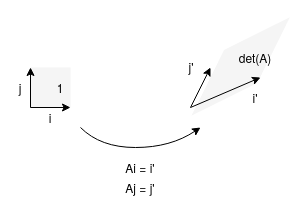
\includegraphics[width=0.4\linewidth]{images/determinant.png}


\paragraph{Definition} \dots

\begin{proof} \label{det_0}
    Let $ A x = 0 $ and $ a \neq 0$. Then it must hold that $\det{A} = 0$.
\end{proof}
We can prove this making use of eq. \ref{lin_indep_if_no_bx0}.

\paragraph{The size of the determinant} can be seen as the scaling-factor of the transformation described by the matrix $A$.

\paragraph{The size of the determinant} is a measure of how much linearly independent the rows/cols of $A$ are. The size of the determinant equals the size of the (hyper-)parallelogram spanned by the columns. If two vectors are almost linearly dependent, they will be almost parallel, leading to a very small area of the parallelogram. So if you have a small determinant, your columns are almost dependent. If you have a large one, your colums are very orthogonal. 













\subsection{The four fundamental subspaces of linear algebra}

We can now print an overview of the different spaces that are associated with a matrix $A$ of dimension $m \cdot n$ and rank $r$.

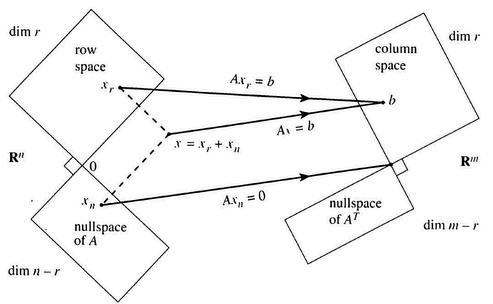
\includegraphics[width=0.7\linewidth]{images/four_spaces.png}

The rowspace of $A$ can be visualized using the line-intersection view of matrix-equations: it contains all the points that lie in the intersection of all the lines that make up the matrix. The columspace of A can be visulaized using the vector-image of A: it contains all the points that are spanned by A. 
Notice how we included the previous theorem: any combination $x$ of a particular sollution $x_r$ and any vector in the nullspace $x_n$ is also a solution.



\subsection{Rank nullity Theorem}

\begin{proof}
    $$ \nullspace{A} = \{ 0 \} \then \det{A} \neq 0 $$
\end{proof}

\begin{proof}
    Let $A: X \to Y$. Then:
    $$ \nullspace{A} = \{ 0 \} \then \collspace{A} = Y $$
\end{proof}

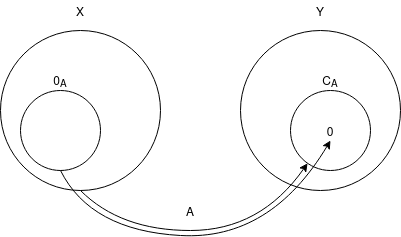
\includegraphics[width=0.4\linewidth]{images/A_from_X_to_Y.png}

\begin{proof}
    Rank nullity: this is a fundamental theorem of linear algebra.
    Let $A$ be of dimension $r \times c$ and full rank.
    Then: 
    $$ r_A + n_A = c $$
\end{proof}


\begin{proof}
    $$ r_A = dim_{C_A} = dim_{R_A} $$
\end{proof}

\begin{proof}
    $$ A:basis_{C_A} \then r_A = n $$
\end{proof}












\subsection{Eigenvalues}

\begin{equation}
    \begin{aligned}
        A x &= \lambda x \\
        ( A - \lambda I ) x &= 0 \\
        \det{A - \lambda I} &= 0 \text{ using eq. \ref{det_0}}
    \end{aligned}
\end{equation}












\subsection{Orthogonal matrices}
TODO: definition orthogonal

\begin{theorem}
    If $A$ is orthogonal, than $A^{-1} = A^T$.
\end{theorem}













\subsection{Inverse}

If $A$ has dimensions $n \times n$, then the inverse $A^{-1}$ such that
$$ A A^{-1} = A^{-1} A = I $$
exists iff $det_A \neq 0$.

\paragraph{Nonsqare} matrices do not have an inverse, but they might have a right- or left-inverse.
Consider $C = A A^T$. This is a square matrix, so it might have an inverse:
$$ A A^T (A A^T)^{-1} = I $$
Calling $A^T (A A^T)^{-1} = A^{RI}$ the right inverse:
$$ A A^{RI} = I $$
For $C^{-1}$ to exist, we require $C$ to be full-rank, which means that $A$ must be full row rank. This  requires $r \leq c$, in other words, $A$ being a broad matrix.

\begin{proof}
If $A^{RI}$ exists, then $A^{LI}$ does not
\end{proof}

\begin{proof}
    $A^{RI}$ is not unique.
    Let $A$ be of dimension $r \times c$ and full rank, with $r < c$. By rank nullity we have
    $$ n_A = c - r > 0 $$
    That is, the nullspace is nonempty. Thus $\thereis x : Ax = 0$
    Now try $B' = B + x$
    We get 
    $$ AB' = AB + Ax = I + 0$$
\end{proof}












\subsection{Change of basis}\label{changeOfBasis}

Let $V$ be a vector space. Let $0$ be the canonical basis for that vector space. Let $A = \{\vec{a}_1, ..., \vec{a}_N \}$ and $B = \{\vec{b}_1, ..., \vec{b}_N\}$ be two other basis for that vectorspace. Let $\mtrx{A}$ be the matrix $[\vec{a}_1  ...  \vec{a}_N]$ and $\mtrx{B} = [\vec{b}_1 ... \vec{b}_N]$

Every vector $\vec{v}$ can be expressed as a linear sum of the basisvectors in $A$, that is $\vec{v} = \sum_n \alpha_n \vec{a}_n$. That same thing in matrix notation: $\vec{v} = \mtrx{A}(\vec{v})_A$, where $(\vec{v})_A$ is the coordinates $\alpha$ of $\vec{v}$ with respect to the basis $A$. Correspondingly, for $B$ we have $\vec{v} = \sum_n \beta_n \vec{b}_n = \mtrx{B}(\vec{v})_B$.

Note that within $A$ and $B$, we express the basevectors with respect to the canonical basis $0$, that is, we should really write $\mtrx{A} = [(\vec{a}_1)_0  ...  (\vec{a}_N)_0]$. Note also that $[(\vec{a}_1)_A  ...  (\vec{a}_N)_A] = \mtrx{I}$, the identity matrix. 

We can use this to obtain a simple formula for the change of basis. 
$$ \vec{v} = \mtrx{A} (\vec{v})_A $$
$$ \vec{v} = \mtrx{B} (\vec{v})_B $$
$$ (\vec{v})_B = \mtrx{B}^{-1} \mtrx{A} (\vec{v})_A $$

But inverses are notoriously hard to calculate. Fortunately, there is another approach. Call $\mtrx{T}_{BA} = [(\vec{a}_1)_B ... (\vec{a}_N)_B]$ the \emph{transition matrix}. We can prove that $\mtrx{B}^{-1} \mtrx{A} = \mtrx{T}_{BA}$:

\begin{equation}
\begin{aligned}
\mtrx{B}^{-1} \mtrx{A} (\vec{v})_A &= \mtrx{T}_{BA}  (\vec{v})_A \\
                                   &= \sum_n (v_n)_A (\vec{a}_n)_B \\
                                   &= \sum_n (v_n)_A \mtrx{B}^{-1} \mtrx{A} (\vec{a}_n)_A \\
                                   &= \mtrx{B}^{-1} \mtrx{A} \sum_n (v_n)_A (\vec{a}_n)_A \\
                                   &= \mtrx{B}^{-1} \mtrx{A} \text{  } \mtrx{I} (\vec{v})_A \\
                    (\vec{v})_A &=  (\vec{v})_A         
\end{aligned}
\end{equation}

Using $\mtrx{T}_{BA} = \mtrx{B}^{-1}\mtrx{A}$, a lot of statements are trivial to prove:
\begin{itemize}
    \item $\mtrx{T}_{BA} = \mtrx{T}_{AB}^{-1}$
    \item $\mtrx{T}_{CA} = \mtrx{T}_{CB} \mtrx{T}_{BA}$
\end{itemize}













\subsection{Linear transformations}

\begin{definition}
Let $U$ and $V$ be two vector spaces and $f:U \to V$. Then $f$ is a \emph{linear transform} if
\begin{itemize}
    \item $f$ preserves scalar multiplication: $f(\alpha \vec{u}) = \alpha f(\vec{u})$
    \item $f$ preserves vector addition: $f(\vec{u}_1 + \vec{u}_2) = f(\vec{u}_1) + f(\vec{u}_2)$
\end{itemize}
\end{definition}

There are a bunch of properties to linear transformations that can be useful to us. 

\begin{proof}[There is a unique linear transform from the basis of $U$ to any set of vectors in $V$ that we want.] In other words, any linear transform $f$ is completely deterimed by the matrix $[ f(\vec{b}_1) ... f(\vec{b}_N) ] = [\vec{v}_1 ... \vec{v}_N]$. That means if we dont know the transform, but we do know the results of the transform on a basis, then we can reconstruct the transform with certainty.  \\

    \subprf{Let $B = \{ \vec{b}_1, ..., \vec{b}_N \}$ be a basis for $U$. Let $\{ \vec{v}_1, ..., \vec{v}_N \}$ be any vectors in $V$ that we may chose. }
    { there is a unique function $f:U \to V$ such that $f(\vec{b}_i) = \vec{v}_i$ }{
    
        \subprf{Try $f(\vec{x}) = \mtrx{V} (\vec{x})_B$}
        {$f(\vec{b}_i) = \vec{v}_i$ and $f$ is a linear transform.}{
        
            \subprf{Part 1: }
            {$f(\vec{b}_i) = \vec{v}_i$}{
                
                $ f(\vec{b}_i) = \mtrx{V} (\vec{b}_i)_B = \mtrx{V} \vec{e}_i = \vec{v}_i $
                
            }
            
            \subprf{Part 2: }{$f$ is unique}{
                
                We could not have obtained any other form of $f$ than $f(\vec{x}) = \mtrx{V} (\vec{x})_B$. This is because for \emph{any} linear transform from $U \to V$ we have: 
                
                $ f(\vec{x}) = f(\mtrx{B}(\vec{x})_B) = f(\sum_n (x_n)_B \vec{b}_n) = \sum_n (x_n)_B f(\vec{b}_n)  $
                
                Using the result from part 1, this cannot be any other function than: 
                
                $ \sum_n (x_n)_B f(\vec{b}_n) = \sum_n (x_n)_B \vec{v}_n = \mtrx{V} (\vec{x})_B $ 
                
            }
            
            \subprf{Part 3: }
            {$f$ is a linear tansform}{
            
            }
        }
    }
\end{proof}

A whole bunch of other properties are now easily proved. Let $f$ and $g$ be linear transforms from $U$ to $V$. The following are also linear transforms: 
\begin{itemize}
    \item $\alpha f$
    \item $f + g$
    \item $f^{-1}$ ( if it exists )
    \item $fg$ ( here $g: V \to W$ )
\end{itemize}

Let $f: U \to V$ be a linear transform. Then the following are equivalent: 
\begin{itemize}
    \item If $f(\vec{u}) = \vec{0}$, then $\vec{u} = \vec{0}$
    \item $f$ is one-to-one
    \item $f$ maps linearly independent vectors to linearly independent vectors. 
\end{itemize}


Prove that a transform can be split up into mulitple transforms on the basis vectors. 
As an examle, consider the case of a rotation. A diagonal rotation can be reproduced by a rotation first around one, then around another axis. 


\paragraph{A linear transformation can also be a change of basis} when it is on a vectorspace and invertible.














\subsection{Applications}


\subsubsection{Systems of linear equations}
If there are more variables than equations, the system is underdetermined. If there are more eqations than variables, the system is overdetermined. A potentially solveable system is one where there are equally many variables as equations. But even then we must distinguish two cases. 

\paragraph{Solving well determined systems}
There are two cases: a system is either consistent or inconsistent. The follwing statements are all equivalent, meaning that any one of them is related to any other one in an if-and-only-if way. 

\begin{itemize}
    \item the system is consistent
    \item the matrix is invertible
    \item the determinant is nonzero
    \item there is exactly one sollution
\end{itemize}

We proof a few of those equivalences just for the hell of it. 

\begin{proof} There is exactly one solution if and only if the determinant is nonzero. \\
    \subprf{}{$|A| = 0 \iff \thereis ! \vec{x} : A \vec{x} = \vec{b} $}{
    
    }
\end{proof}

On the other hand, in the inconsistent case, the follwing statements are equivalent:

\begin{itemize}
    \item the system is inconsistent
    \item the matrix is singular (aka. noninvertible)
    \item the determinant equals zero
    \item one (or more) row (or column) is lineraly dependent of the others
\end{itemize}

\paragraph{Solving overdetermined systems: least squares}


\paragraph{Solving underdetermined systems: geometric bodies}
I like to think of underdetermined systems as (linear) geometric bodies, written in their parameterized form. A line in $\reals^3$ is described by a $3 \times 1$ matrix (or rather, it's column space), a plane in $\reals^3$ by a $3 \times 2$ matrix. However, it is important to note one distinction: geometric objects don't need to go through the origin, a matrix system however does. A line that does not go through the origin needs a base vector, like so: 

$$\vec{x} = \begin{bmatrix} \vec{d} \end{bmatrix} \begin{bmatrix} \alpha \end{bmatrix} + \vec{b}$$ 

A plane that does not go through the origin also needs a base vector $\vec{b}$, like so: 

$$\vec{x} = \begin{bmatrix} \vec{p}_1 && \vec{p}_2 \end{bmatrix} \begin{bmatrix} \alpha  \\ \beta \end{bmatrix} + \vec{b}  $$



Here is a problem that bothered me for a while: a line needs one parameter, a plane two. An ellipsoid, too, needs two parameters. Are there any linear geometric objects in $\reals^3$ that require more than three parameters? The answer is: no. Here is the proof. 

\begin{proof}
    For any $3 \times 4$ matrix, there is a $3 \times 3$ matrix that has the same column space, that is, that describes the same geometrical body. \\
    
    \subprf{}{$\forall A(3 \times 4) \thereis A'(3 \times 3): \collspace{A} = \collspace{A'}$}{

        \subprf{Let $A_0(3 \times4)$.}{$\thereis A': \collspace{A_0} = \collspace{A'}$}{
        
            We know from \ref{proofBaseSizeEqualsSpaceDimension} that $\thereis \vec{a}_0 \in A_0: \vec{a}_0:ld$. So Try $A' = A_0/\vec{a_0}$.
            
            Indeed, now $A_0$ and $A'$ both form a base of the same space. So they must have the same column space. 
        }    

    }
\end{proof}

However, there are \emph{non}linear objects in $\reals^3$ that require more than three parameters! Many curves in 3d require many parameters. \emph{But} those curves don't form a vector-space, while lines and planes do (as long as they go through the origin). 


\paragraph{Summary}
\begin{table}[ht]
\centering
\caption{Influence of rank on solutions}
\begin{tabular}{@{}llll@{}}
\toprule
                                                                                      & m \textless n                             & m = n & m \textgreater n                                 \\ \midrule
\rowcolor[HTML]{96FFFB} 
\cellcolor[HTML]{96FFFB}                                                              & n - m free variables                      &       &                                                  \\
\rowcolor[HTML]{96FFFB} 
\multirow{-2}{*}{\cellcolor[HTML]{96FFFB}r \textless m}                               & m – r conditions on $b \in \collspace{A}$ &       &                                                  \\
                                                                                      & 1 pivot per row                           &       &                                                  \\
                                                                                      & n – r = n – m free variables              &       &                                                  \\
\multirow{-3}{*}{\begin{tabular}[c]{@{}l@{}}r = m \\ (full row rank)\end{tabular}}    & 0 conditions on $b \in \collspace{A}$     &       & X                                                 \\
\rowcolor[HTML]{96FFFB} 
\cellcolor[HTML]{96FFFB}                                                              &                                           &       & m – r conditions on $b \in \collspace{A}$        \\
\rowcolor[HTML]{96FFFB} 
\multirow{-2}{*}{\cellcolor[HTML]{96FFFB}r \textless n}                               &                                           &       & n – r free variables                             \\
                                                                                      & X                                         &       & 1 pivot per column                               \\
                                                                                      &                                           &       & m – r = m – n conditions on $b \in \collspace{A}$ \\
\multirow{-3}{*}{\begin{tabular}[c]{@{}l@{}}r = n \\ (full column rank)\end{tabular}} &                                           &       & 0 free variables, thus $\nullspace{A} = \{0\}$     \\ \cmidrule(l){1-4} 
\end{tabular}
\end{table}




\paragraph {Ax = b reduces to A'x' = 0}

\begin{theorem}
  A problem of the form $Ax = b$ can be re-expressed as $A'x' = 0$, where $A' = [A, -b]$ 
\end{theorem}

\begin{proof}
    \subprf {} {$A x = b$ can be re-expressed as $A'x' = 0$} {
        $ A x = b $ \\
        $ A x -b = 0 $ \\
        $ A_1 x_1 + A_2 x_2 + ... -b = 0 $ \\
        Let $A' = [A, b]$ and $x_{n+1} = -1$. Then: \\
        $ A' x' = 0 $ \\
        Now we can use the nullspace of $A'$ to find the solutionspace of $A$. \\
        $ \nullspace{[A b]} = \{x' | [A b]x' = 0\} $ \\
        $ = \{x' | A x'_{1:m} = -b x'_{m+1}\} $ \\
        A subset of that nullspace equals the solutionset for $A x = b$: \\
        $ \nullspace{[A b]}_{[x'_{m+1} = -1]} = \{x'| A x'_{1:m} = b \} $ 
    }   
\end{proof}


\paragraph{Solving Ax = b}

\begin{theorem}
  If we can only find any one particular solution $x_p$ such that $A x_p = b$, then we get the whole solutionspace as $\nullspace{A} + x_p$.
\end{theorem}

\begin{proof}
    \subprf{Let $x_p: A x_p = b$.}{$\solspace{A x = b} = \nullspace{A} + x_p$}{
        We'll make use of the fact that $\nullspace{A} + x_p = \{ x + x_p | A x = 0 \} = \{ x | A x = A x_p \}$ \\
        \subprf{Let $x_0 \in \nullspace{A} + x_p $.}{$x_0 \in \solspace{A x = b}$, i.o.w. $A x_0 = b$}{
            $ x_0 \in \nullspace{A} + x_p $ \\
            $ x_0 \in \{ x + x_p | A x = 0 \} $ \\
            $ x_0 \in \{ x | A (x - x_p) = 0 \} $ \\
            Thus $ A x_0 = A x_p $ \\
            Since $A x_p = b$, it must be that $ A x_0 = b $.
        }
        \subprf{Let $x_0 \in \solspace{A x = b}$.}{$x_0 \in \nullspace{A} + x_p$, i.o.w. $A x_0 = A x_p$}{
            Because $x_0 \in \solspace{A x = b}$, we have $A x_0 = b$. \\
            Also, it was given that $A x_p = b$.
        }
    }
\end{proof}





\subsubsection{Matrix factorisation}

\paragraph{Eigenvalue decomposition}

$$ A = V \Lambda V^{-1} $$

\paragraph{Singular value decomposition} is eigenvalue decomposition, generalized to non-square matrices.
Getting the basis for $\nullspace{A}$ becomes numerically feasible using singular value decomposition.

$$ A = U \Sigma V^T $$

SVD is related to EVD like this: 

\begin{equation}
    \begin{aligned} 
        A^T A &= V \Sigma^T U^T U \Sigma V^T \\
              &= V \Sigma^T \Sigma V^T
    \end{aligned}
\end{equation}

This makes the entries of $\Sigma$ the squares of the eigenvalues of the matrix $A$.

\paragraph{Nonnegative matrix factorisation}: Consider a dataset $A$, mapping people (rows) to properties (columns). You are looking for some hidden, small set of features, that groups of people have in common. 
In neural networks we can reconstruct images from a minimal amount of hidden features by funnelling the image through a very small hidden layer out to a large output layer. We can do the very same thing here!
$$ A = U V $$
Where $A$ has dimension $r \times c$, $U$ associates people with their hidden features/groups $r \times f$ and $V$ associates features/groups with the properties $f \times c$.

\section{Geometric algebra}

The geometric algebra is the algebra of multivectors. multivectors form a vectorspace, an inner product space and an algebra. 

\subsection{Definition of the algebra}
The geometric algeba has elements 
$$A = scalar + vector + plane + volume + ... = (A)_0 + (A)_1 + (A)_2 + (A)_3 + ...$$

It can be proven that such an algebra exists with the following gemoetric product: 
\begin{itemize}
    \item $AB \in \geometrics^n$
    \item $A(B+C) = AB + BC$
    \item $(A + B)C = AC + BC$
    \item $(\alpha A)B = A(\alpha B) = \alpha (AB)$
    \item $(AB)C = A(BC)$
    \item $1A = A1 = A$
\end{itemize}


\subsection{Canonical basis}
In $\geometrics^2$, this basis would consist of $1, e_1, e_2, e_1e_2$.

A little slang is in order: 
\begin{itemize}
    \item a k-vector is a multivector consisting only of rank-j elemens. For example, a 2 vector in $\geometrics^3$ could be written as $a = \alpha e_1e_2 + \beta e_2e_3 + \gamma e_3e_1$
\end{itemize}

\subsection{Geometric product}
Let's inspect the case of $\geometrics^1$.

\begin{equation}
    \begin{split}
        A &= \alpha_0 + \alpha_1 e \\
        B &= \beta_0 + \beta_1 e \\
        AB &= (\alpha_0 + \alpha_1 e)(\beta_0 + \beta_1 e) \\
          &= (\alpha_0 \beta_1 + \alpha_1 \beta_0) + (\alpha_1 \beta_0 + \alpha_0 \beta_1) e \\
    \end{split}
\end{equation}


\subsubsection{Inner product}
The inner product of a j-vector A and a k-vector B is:
$$ A \innerprod B = (AB)_{\rank{B} - \rank{A}} $$

\subsubsection{Outer product}
The outer product of a j-vector A and a k-vector B is: 
$$ A \outerprod B = (AB)_{\rank{A} + \rank{B}}$$

\subsubsection{Norm and inverse}

The reverse of a k-vector $A = a_1 a_2 ... a_k$ is $A^\dagger = a_k ... a_2 a_1$. This equals $A^\dagger = (-1)^{k(k-1)/2} A$. 

The norm of a multivector is defined as 
$$ A = \sum_J \alpha_J e_J \then |A| = \sum_J \alpha_J^2 $$
If $A$ is a k-vector $A = a_1 a_2 ... a_k$, then the inverse of $A$ is 
$$ A^{-1} = \frac{(-1)^{k(k-1)/2}}{|A|^2} A $$
If $B$ isn't a k-vector, then it can be expressed as as sum of k-vectors. But be careful: the norm is not a linear function. So $|B| = |\sum_j A_j| \neq \sum_j |A_j|$


\subsubsection{Parallel and orthogonal part}

\subsection{Fourier decomposition of multivectors}
Every multivector can be written in the form
$$ A = \sum_J (e_J^{-1}A)_0 e_J$$
This is easily proven. 
\begin{equation}
    \begin{split}
        A &= \sum_J \alpha_J e_J \\
        (A e_I)_0 &= \sum_J \alpha_J (e_J e_I)_0 \\
                &= \alpha_I
    \end{split}
\end{equation}

If a is a vector, this reduces to the normal 
$$ a = \sum_j (a \innerprod e_j) e_j$$


\subsection{Geometric calculus}



\section{Fourier and Laplace}

\begin{figure}[H]
  \caption{Time Base versus Fourier Base}
  \centering
    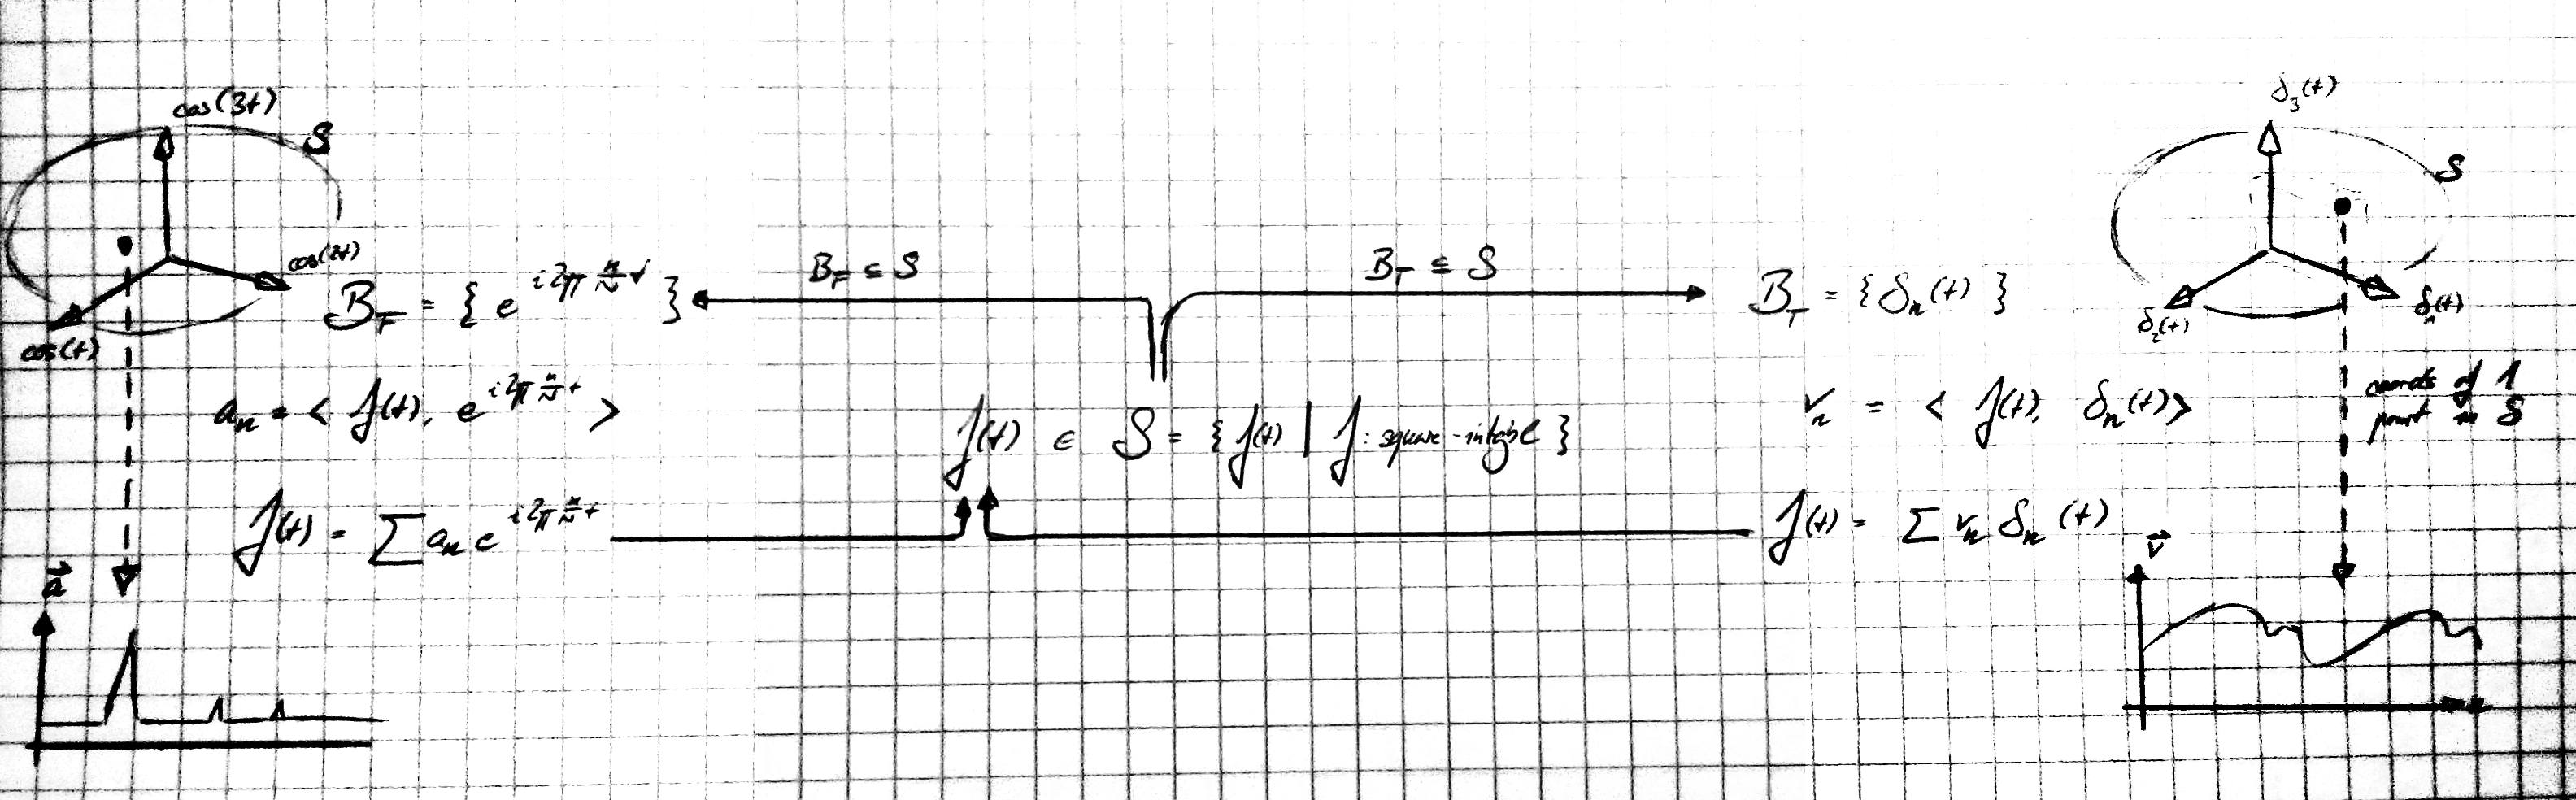
\includegraphics[width=0.95\textwidth]{images/fourier_base.jpg}
\end{figure}


\subsection{Discrete Fourier Analysis}

We'll begin with the discrete case. For one, this case is the basis of the FFT. Also, the math is a lot easier in the discrete case. Let $N$ be the samplesize and $\delta$ be the samplefrequency (often equal to 44100 Hz or 48000 Hz). Let $V$ be the samplespace of signals of size $N$. This is a vectorspace, equipped with an inner product of the form $\innerprodbr{\vec{a}}{\vec{b}} = \frac{1}{N} \sum_{k=0}^{N-1} a_k (b_k)^*$, where $()^*$ is the complex complement.

\subsubsection{The Fourier Base}




We'll use the base $B = \{ \vec{w}_N^n | n \in [0, N-1]\}$. Here, $\vec{w}_N^n$ is the vector we get by evaluating $e^{i 2\pi \frac{n}{N} k}$ at the points $k=0, k=1, ..., k=N-1$. Thus if we call $w_N = e^{i 2 \pi \frac{1}{N}}$, then the vector $\vec{w}_N^n$ consists of the elements $w_N^{nk}$. Throughout this chapter, $k$ will be the index of time/the signalvector and $n$ will be the index of frequency/the basevectors.

In the case of $N = 4$ we obtain the matrix:
$$ \left[\begin{matrix}e^{0.25 i \pi} & e^{0.5 i \pi} & e^{0.75 i \pi} & e^{1.0 i \pi}\\e^{0.5 i \pi} & e^{1.0 i \pi} & e^{1.5 i \pi} & e^{2.0 i \pi}\\e^{0.75 i \pi} & e^{1.5 i \pi} & e^{2.25 i \pi} & e^{3.0 i \pi}\\e^{1.0 i \pi} & e^{2.0 i \pi} & e^{3.0 i \pi} & e^{4.0 i \pi}\end{matrix}\right] $$
Note that fourier bases are symmetric matrices. 

The Fourier-base is a very particular choice: each element of each base-vector turns out to be one of the $N$ complex $N$th roots of one. We could have chosen any base-vectors, but these complex roots will turn out to have a few useful properties that we will exploit to speed up the Fourier transformation. These properties are:

\begin{enumerate}
    \item $w_N^x = (w_N)^x$
    \item $w_N^{2x} = w_{N/2}^x$
    \item $w_N^{2x+N} = w_N^{2x}$
    \item $w_N^{x+N/2} = - w_N^x$
\end{enumerate}

It is also easy to prove that this base is orthogonal.
\begin{proof} The vectors $\vec{w}_N^n$ are orthogonal. \\
\subprf{Suppose $n \neq m$.}
    {$\innerprodbr{\vec{w}_N^n}{\vec{w}_N^m} = 0$ }{
    
    $\innerprodbr{\vec{w}_N^n}{\vec{w}_N^m} = \frac{1}{N} \sum_{k=0}^{N-1} e^{i 2\pi \frac{n-m}{N} k} $ \\
    
    Using the result $\sum_{n=0}^{N-1} e^{xn} = \frac{1-e^{xN}}{1-e^{x}}$, we find: \\
    
    $\frac{1}{N} \sum_{k=0}^{N-1} e^{i 2\pi \frac{n-m}{N} k} = \frac{1}{N} \frac{1-e^{i 2\pi (n-m)}}{1-e^{i 2\pi \frac{n-m}{N}}}$ \\
    
    It is easy to see that $e^{i 2\pi (n-m)} = 1$. So the above term must equal 0.
    
    
}
\subprf{Suppose $n = m$.}
    {$\innerprodbr{\vec{w}_N^n}{\vec{w}_N^m} = 1$ }{

    We use the same line of reasoning as above to obtain: \\
    
    $ \innerprodbr{\vec{w}_N^n}{\vec{w}_N^m} = \frac{1}{N} \frac{1-e^{i 2\pi (0)}}{1-e^{i 2\pi \frac{0}{N}}}$ \\
    
    In the limit, this equals 1.
}
\end{proof}


Proof of spanning

\subsubsection{Obtaining the amplitudes}
After having proven that $B$ is an orthonormal base for $V$, we can get to the core of the Fourier analysis: given a signal $\vec{v}$, how do we obtain the amplitudes in $\vec{v} = \sum_{n=0}^{N-1} \alpha_n \vec{w}_n$ ? Well, from paragraph \ref{fourierDecomposition} we know that 

$$ \alpha_n = \innerprodbr{\vec{v}}{\vec{w}_N^n} = \frac{1}{N} \sum_{k=0}^{N-1} v_k e^{i 2\pi \frac{n}{N} k} $$

Using Horners method, this is a \BigTheta{n} operation. Executing it on all $n$ coefficients, the whole proces becomes a \BigTheta{n^2} operation. A naive implementation might look like this: 

\begin{lstlisting}[language=python]
import numpy as np

def amplitudes(signal):
    N = len(signal)
    amps = []
    for n in range(N):
        sm = 0
        for k in range(N):
            wnk = np.exp(-1j * 2 * np.pi * n * k / N) 
            sm += signal[k] * wnk
        amps.insert(n, sm/N)
    return amps


sig = [2, 1, 1, 4]
print amplitudes(sig)
\end{lstlisting}

Notice that this is a matrix operation. 


\subsection{As a matrix operation}

\begin{proof}
    The Fourier transform of $\vec{a} + \vec{b}$ equals the transform of $\vec{a}$ plus the transform of $\vec{b}$

    Note that the Fourier transform can be rewritten in matrix form. 
    
    $$
    <\vec{a}, \vec{f}_m>(m) = 
    \begin{bmatrix} f_{1,1} & ... & f_{F,T} \\ ... & & ... \\ f_{F,1} & ... & f_{1,T}  \end{bmatrix} 
    \begin{bmatrix} a_1 \\ a_2 \\ ... \\ a_T \end{bmatrix}  
    = 
    \begin{bmatrix} <\vec{a}, \vec{f}_1> \\ <\vec{a}, \vec{f}_2> \\ ...  \\ <\vec{a}, \vec{f}_F> \end{bmatrix} 
    $$
    
    This means that the rules for matrix multiplication apply to the Fourier transformation, amongst which that matrix multiplication is distributive:
    
    $$ A (\vec{a} + \vec{b}) = A \vec{a} + A \vec{b} $$
    
    Remember that a matrix-multiplication is always a change of basis: the vector $\vec{v}_I$ (as displayed in the euclidian system $\mtrx{I}$) can also be expressed relative to the Fourier-base $\mtrx{F}$ as $\vec{v}_F$. 
    $$ \mtrx{F}^{-1} \vec{v}_I = \vec{v}_F $$
    where (according to \ref{changeOfBasis}): 
    $$ \mtrx{F}^{-1} = \begin{bmatrix} \vec{x}_F & \vec{y}_F & \vec{z}_F \end{bmatrix} $$
    
\end{proof}


\subsection{Fast Fourier Transform}

In the previous section we have evaluated the polynomal $\sum_{k=0}^{N-1} v_k e^{i 2 \pi \frac{n}{N} k}$ like this:
\begin{lstlisting}[language=python]
for k in range(N):
    wnk = np.exp(1j * 2 * np.pi * n * k / N) 
    sm += signal[k] * wnk
\end{lstlisting}

Really, this is just the same as evaluating the polynomal $A(x) = \sum_{k=0}^{N-1} v_k x^k$, where $x = e^{i 2 \pi \frac{n}{N} 1} = w_N^n$ (using property 1). In other words, we calculated $A(w_N^n)$.

However, it turns out that we can simplify this process. Before we detail how exactly this section is to be simplified, we need to realize that for any polynomal $A(x)$, it holds that $A(x) = A_{even}(x^2) + x A_{odd}(x^2)$


Knowing that, we can split the evaluation in half:
$$ A(w_N^n) = A_{even}(w_N^{2n}) + w_N^n A_{odd}(w_N^{2n})$$


And using the properties 2-4 of $w_N^n$, we can calculate:
\begin{equation} 
\begin{split} 
    A(w_N^n) & = A_{even}(w_N^{2n})   + w_N^n A_{odd}(w_N^{2n})   \\
             & = A_{even}(w_{N/2}^n)  + w_N^n A_{odd}(w_{N/2}^n)
\end{split}
\end{equation}

\begin{equation} 
\begin{split}  
A(w_N^{n + N/2})  & = A_{even}(w_N^{2n+ N}) + w_N^{n+N/2} A_{odd}(w_N^{2n + N}) \\
                  & = A_{even}(w_N^{2n}) - w_N^n A_{odd}(w_N^{2n})   \\
                  & = A_{even}(w_{N/2}^n) - w_N^n A_{odd}(w_{N/2}^n)
\end{split}
\end{equation}

This way, we obtain:
\begin{lstlisting}[language=python]
def fft(signal):
    N = len(signal)

    if N == 1:
        return signal

    sigE = []
    sigU = []
    for k in range(N):
        if k%2 == 0:
            sigE.append(signal[k])
        else:
            sigU.append(signal[k])

    ampsE = fft(sigE)
    ampsU = fft(sigU)

    amps = []
    for n in range(N/2):
        wn = np.exp(-1j * 2 * np.pi * n / N)
        an   = ampsE[n] + wn * ampsU[n]
        an2N = ampsE[n] - wn * ampsU[n]
        amps.insert(n,       an   )
        amps.insert(n + N/2, an2N )

    return amps
\end{lstlisting}

\subsubsection{Backtransformation}

\subsection{Fourier for musical frequencies}
Musical notes are special. Here, we don't want to get the full spectrum that FFT delivers, but only a few selected frequencies. 
\subsubsection{Goertzel}
Goertzel continues to work with the Fourier base. It differs from FFT in that only a few of the elements that FFT returns are actually evaluated. 
\subsubsection{PCI}
PCI (pre-calculated inverse algorithm) discards of the Fourier base and instead uses the musical frequencies in the base. This results in a non-orthogonal base, but that won't hinder us. 
\begin{equation}
    \begin{split}
        \vec{s} &= \sum_F a_f e^{-2 \pi i f t} \text{  , with F = \{440, 465, ...\}}  \\
                &= \begin{bmatrix}  ... & & ... \\ & e^{- 2 \pi i f t} & \\ ... &  & ... \end{bmatrix} \vec{a} \\
        \vec{a} &= \begin{bmatrix}  ... & & ... \\ & e^{- 2 \pi i f t} & \\ ... &  & ... \end{bmatrix}^{-1} \vec{s}
    \end{split}
\end{equation}

\subsection{Continuous Fourier Analysis}

In Fourier analysis, we deal with the innerproduct space $C_{[a,b]}^2$: the space of square-integrable functions that are continuous from $a$ to $b$. An orthogonal base for this vectorspace would be the Fourier base $\{ sin(\frac{j 2 \pi}{b-a} t), cos(\frac{j 2 \pi}{b-a}  t) | j \in \naturals \}$. Often, making use of Eulers formula, we instead write this base as $\{ e^{i \frac{n 2 \pi}{b-a} t} | j \in \naturals \}$. 

\subsubsection{Comparing Fourier to other important series}

\paragraph{Fourier versus Taylor} Another famous expansion of functions is the Taylor-expansion. It is important to note that the Taylor expansion is a completely different beast from the Fourier expansion.

\begin{itemize}
    \item Taylor works on locally differentiable functions, whereas Fourier works on globally integrable functions. You cannot recover the full function from its Taylor-expansion.
    
    \item The Taylor-base is non-orthogonal\footnote{proof required}
\end{itemize}

\begin{table}[ht]
\centering
\caption{Fourier versus Taylor}
\begin{tabular}{@{}lll@{}}
\toprule
        & coefficients                                              & basevectors                       \\ \midrule
Fourier & $f(t) \innerprod e^{i \frac{n 2 \pi}{b-a} t}$             & $e^{i \frac{n 2 \pi}{b-a}  t}$    \\
Taylor  & $f^{(n)}(t)|t_0$                                          & $\frac{(x- x_0)^n}{n!}$          
\end{tabular}
\end{table}

\paragraph{Fourier versus PCA} PCA comes a lot closer to Fourier in that in PCA we represent our data as a linear combination of orthogonal base-vectors. There are two differences though. In PCA the data is usually a matrix instead of a vector. And in PCA we don't know in advance what the set of base-vectors is going to be, but much rather chose the most fitting one for our datamatrix. It turns out that we can use the set of eigenvectors of the datamatrix\footnote{Strictly speaking, we don't work with the raw datamatrix, but rather its correaltion matrix. This is because for the eigenvector thing to work , we need the matrix to be symetric and centered around the origin, which the raw data matrix usually isn't.}.

\begin{proof}There is a set of eigenvectors $E$ of a matrix $M$ that is an orthogonal basis for $\solspace{M}$
    \subprf{}{}{}
\end{proof}



\subsubsection{Proving that Fourier functions form a basis}

We can use Fourier to describe any functionspace - if we can prove that the Fourier functions do indeed form a basis for that space. This takes two steps: proving orthogonality and proving span.

\paragraph{Orthogonality} This is very straightforward: 

\paragraph{Span} This  requires more work.  We're first going to have to prove The Weierstrass-Theorem. This theorem states that the set $B = \{ x^j | j \in \naturals \}$ forms a basis for $C_{[a,b]}$.
https://psychedai.wordpress.com/2016/11/15/the-intuition-behind-bernsteins-proof-of-the-weierstrass-approximation-theorem/


\subsubsection{Fourier transform on vector valued functions}
As long as a vector-valued function can be decomposed over a set of basis-vectors (never mind what basis vectors exactly, this works with any basis), we can still use the normal, scalar Fourier transform on them. 
\begin{equation}
    \begin{split}
        g &: A^N \to A^M \\
        g(\vec{x}) &= \sum_m^M g_m(\vec{x}) \vec{e}_m \text{ ... decomposing the function over the output basis} \\
        \fourier_g(\vec{u}) &= \sum_m^M \vec{e}_m \fourier_{g_m}(\vec{u})  \text{ ... Fourier transform over the input basis}
    \end{split}
\end{equation}

Consider the example of a rgb-image.
\begin{equation}
    \begin{split}
        c(x,y) &= \vec{e}_1 r(x,y) + \vec{e}_2 g(x,y) + \vec{e}_3 b(x,y) \\
        \fourier_c\begin{bmatrix} f_x \\ f_y \end{bmatrix} 
                        &= \int_X \int_Y c(x,y) e^{-2\pi i (f_xx + f_yy)} \diff{y} \diff{x} \\
                        &= \int_X \int_Y \vec{e}_1 r(x,y) e^{-2\pi i (f_xx + f_yy)} \diff{y} \diff{x} + ... \\
                        &= \vec{e}_1 \fourier_r\begin{bmatrix} f_x \\ f_y \end{bmatrix} + \vec{e}_2 \fourier_g\begin{bmatrix} f_x \\ f_y \end{bmatrix} + \vec{e}_3 \fourier_b\begin{bmatrix} f_x \\ f_y \end{bmatrix} 
    \end{split}
\end{equation}

Note that the resulting fourier spectrum consist of complex 3d-vectors.

Sometimes, however, you either have an input function that contains \emph{multivector} elements, or you want to apply a filter to the fourier spectrum based on mulitvectors. In that case, you can find an introduction to geometric-algebra Fourier transforms here: \inlinecode{https://pdfs.semanticscholar.org/41ce/67428ee60748a4142dee0eea28ed997855e6.pdf}
%\section{Group theory}
\section{Graphics}

\subsection{Points}

Distance in 1-D:
$$ d = \Delta x $$

Distance between two points in 2-D: 
$$ d = \sqrt{\Delta x^2 + \Delta y^2} $$

Distance between two points in 3-D:
$$ d = \sqrt{ \sqrt{\Delta x^2 + \Delta y^2}^2 + \Delta z^2 } = \sqrt{\Delta x^2 + \Delta y^2 + \Delta z^2}$$


\subsection{Geometric objects in matrix notation}

$x=1$ defines a plane, as does $x=2y$. $x=1 \land y=2$ defines a line. 
More generally, the dimension of a geometrical object equals 3 minus the number of equations needed to describe the object.
Informally written: $ dim(obj) = 3 - \#(=) $.

In more rigorous terms, the "number of equations needed to describe the object" is called the rank of the matrix. 3 in our case is the dimension of the space. The geometrical object is really the column-space of the matrix. 


\subsubsection{Plane}

Defined by one point $\vec{b}$ and two lines $\vec{p_1}, \vec{p_2}$: 
$$ P = \{ \vec{x} | \thereis a,b:  \vec{x} = \vec{b} + a\vec{p_1} + b\vec{p_2} \} $$

Or defined by one point $\vec{b}$ and one normal $\vec{n}$:
$$ P = \{ \vec{x} | ( \vec{x} - \vec{b} )\cdot \vec{n} = 0 \} $$


\subsubsection{Line}

Defined by two points: 
$$ L = \{ \vec{x} | \thereis \alpha:  \vec{x} = \vec{b} + \alpha \cdot \vec{\Delta}  \}$$

Or transformed in matrix-notation:
$$ 
\vec{x} = 
\begin{bmatrix}
    \vec{b} & \vec{\Delta}
\end{bmatrix}
\cdot
\myarray{ 1 \\ \alpha }
$$

$$
\begin{bmatrix}
    \vec{b} & \vec{\Delta}
\end{bmatrix}^{-1}
\cdot
\vec{x} = 
\myarray{ 1 \\ \alpha }
$$


\subsubsection{Intersection Line/Plane}

Substituting the definition of a line into the definition of a plane we get:

$$ ( \vec{b_l} + \alpha \cdot \vec{\Delta} - \vec{b_p} )\cdot \vec{n} = 0 $$

This reduces to: 

$$ \alpha = \frac{ ( \vec{b_l} - \vec{b_p} ) \cdot \vec{n} }{ \vec{\Delta} \cdot \vec{n} } $$

Alternatively, we can make use of the two-line-definition of the plane and obtain: 

$$ \vec{b} + a\vec{p_1} + b\vec{p_2} = \vec{b} + \alpha \cdot \vec{\Delta} $$

$$ \vec{b_l} - \vec{b_p} = \myarray{ \vec{p_1} & \vec{p_2} & \vec{\Delta} } \myarray{a \\ b \\ \alpha} $$

\subsection{Projections}

\subsubsection{Finding a perpendicular}

Having a vector $\vec{a}$, how do we find a vector $\vec{a^T}$ that has the following properties:
\begin{itemize}
    \item $ \vec{a} \cdot \vec{a^T} = 0 $
    \item $ | \vec{a} | = | \vec{a^T} | $
\end{itemize}

These two requirements can be re-expressed as 
\begin{itemize}
    \item $ ax + by = 0 $
    \item $ x^2 + y^2 = a^2 + b^2 $
\end{itemize}
This is a nonlinear system, but still solveable. Indeed, we quickly find: 

$$ \vec{a^T} = \myarray{ -y \\ x } $$


How about the two perpendiculars to a 3d-vector? You can just use \myarray{-y & x & 0 } and \myarray{0 & -z & y}. All possible perpendiculars will be linear combinations of these two.


\subsubsection{Projecting one vector onto another}

Imagine we wanted to know $\alpha$ in the following graphic:

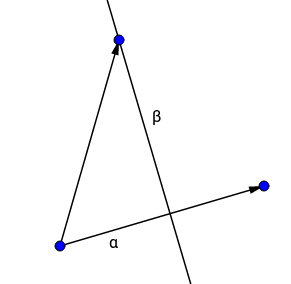
\includegraphics[scale=0.5]{projection.png}

Here, $\alpha$ is the length of vector $\vec{b}$ projected onto $\vec{a}$. How can we find $\alpha$?

The solution lies in imagening the vector $\vec{b}$ being expressed inside a coordinate-system consisting of $\vec{a}$ and $\vec{a^T}$, like so: 

$$ [ \vec{a}, \vec{a^T} ] \myarray{ \alpha \\ \beta } = \vec{b} $$

\subsection{Rotation}

\subsubsection{In 2d}
To find the rotation matrix $\mtrx{R}_2$  in 2d, you could take the naive approach by taking a generic vector $\begin{bmatrix}x \\ y\end{bmatrix}$ and try to solve this equation: 
\begin{align}
    r = \sqrt{x^2 + y^2} \\
    \theta_0 = \cos^{-1}(x/r) \\
    \mtrx{R}_2 \begin{bmatrix}x \\ y\end{bmatrix} = \begin{bmatrix} 
        r \sin(\theta + \theta_0) \\
        r \cos(\theta + \theta_0)
    \end{bmatrix}
\end{align}
While this is a feasible approach, we can have it much easier. Remember from \ref{changeOfBasis} that 
$$ \vec{v} = \mtrx{T} \vec{v}_T $$
If T is invertible:
$$ \vec{v}_T = \mtrx{T}^{-1} \vec{v} $$
Where:
$$ \mtrx{T}^{-1} = [\vec{x}_T, \vec{y}_T, ...] $$
Specifically, in our case this results in 
$$ \mtrx{R}_2 = \begin{bmatrix} 
    \cos{\theta} & -\sin{\theta} \\
    \sin{\theta} & \cos{\theta}
\end{bmatrix} $$

\subsubsection{In 3d}
While in 2d we only had one axis to rotate around, in 3d we can chose if we want to rotate around x, y, or z. In the general case: 
$$ \mtrx{R}_3 = \mtrx{R}_x \mtrx{R}_y \mtrx{R}_z $$. 
It is easy to obtain $\mtrx{R}_z$, the rotation around the z-axis. Just imagine you viewed everything from above:
$$ \mtrx{R}_x = \begin{bmatrix}
    \cos{\theta} & -\sin{\theta} & 0 \\
    \sin{\theta} & \cos{\theta}   & 0 \\
    0            & 0             & 1
\end{bmatrix}$$
This way we obtain 
$$ $$

\subsubsection{Why is there one rotation axis in 2d, but 3 in 3d?}
The rotation axis for any pair of axii that define a plane in space is a third axis perpendicular to that plane. In conventional 2D (XY plane), all rotation is done in the Z axis. 
But what about spherical coordinates? There we need only two angles! ...

\subsection{Implicit versus parameterized representation of bodies}

In geometry, we often represent bodies in set-notation, aka. implicit notation. Consider for example the ellipsoid: 

$$ \left \{\vec{v} | \frac{x^2}{r_1^2} + \frac{z^2}{r_2^2} + \frac{z^2}{r_3^2} = 1 \right \}$$

This body can be parameterized as: 

$$ \begin{bmatrix}
x \\
y \\
z
\end{bmatrix} = 
\begin{bmatrix}
r_1 \cos{\theta} \cos{\phi} \\
r_2 \cos{\theta} \sin{\phi} \\
r_3 \sin{\theta}
\end{bmatrix} $$

In the set notation, the ellipsoid had no parameters (it had $r_1, r_2, r_3$, but these are \emph{constants}). With $\theta$ and $\phi$ we now found two parameters which, when varied over their whole domain $[0\degree, 360\degree]^2$, yield every point in the set. 


Parameterisation means \emph{finding a function of one or more parameters who's range equals the set}. That means nothing other than \emph{putting the vector $\vec{x}$ on the left side}. Conversely, you have an \emph{implicit} equation when you can write the equation such that the left side is $0$ (for clarity: we mean the number $0$, not a zero-vector).


As a sidenote, when you find a set-expression of a body that contains a $thereis$ statement, chances are that this statement already \emph{is} parameterized.


\begin{table}[H]
\centering
\caption{Explicit and parametric set of plane and ellipsoid}
\begin{tabular}{c|cc}
           & implicit                                                 & parametric \\
\hline 
linear     & $\left \{\vec{x} | ( \vec{x} - \vec{b} ) \dot \vec{n} = 0 \right \}$  & $\left \{\vec{x} | \thereis \alpha, \beta: \vec{x} = \begin{bmatrix} \vec{b} && \vec{p}_1 && \vec{p}_2 \end{bmatrix} \begin{bmatrix} 1 \\ \alpha \\ \beta \end{bmatrix}  \right \}$ \\
non-linear & $\left \{\vec{x} | \frac{x^2}{r_x} + \frac{y^2}{r_y} + \frac{z^2}{r_z} = 1 \right \}$ &  $\left \{\vec{x} | \thereis \theta, \phi: \vec{x} = \begin{bmatrix} r_x \cos{\theta} \cos{\phi} \\ r_y \cos{\theta} \sin{\phi} \\ r_z \sin{\theta} \end{bmatrix} \right \}$       
\end{tabular}
\end{table}

We can find more about this topic here: https://en.wikipedia.org/wiki/Implicit\_surface. In this section, we have been careful to never mention the term \emph{explicit}. In this section, we dealt with bodies. But if we only wanted surfaces, that is, bodies where there are never two z values at on x/y spot, there is also the explicit representation $z=f(x,y)$.

\begin{table}[H]
\centering
\caption{Overview of implicit, explicit and parameterized functions}
\begin{tabular}{l|ll|r}
              & in         & out     & notes                                 \\
              \hline
implicit      & x, y, z    &         &                                       \\
explicit      & x, y       & z       & doesn't allow more than one z per x/y \\
parameterized & $\theta, \phi$ & x, y, z &                                      
\end{tabular}
\end{table}

%One neat fact is this: 
%\begin{itemize}
%    \item Take the parameterized version of a body.
%    \item This version can be written as a matrix equation $Ax = b$, by putting all things that can vary %into $x$.
%    \item Calculate the degrees of freedom of this matrix equation: $dof = \#cols - \#rows$.
%    \item The $dof$ equals the minimal amount of parameters that you need to write the parameterized %equation of the body. 
%\end{itemize}
%
%How does one find the minimum amount of parameters for a body, whether it's given implicitly versus explicitly? 
%For an implicit example, consider the case of the ellipsoid again. 
%
%\begin{align*}
%    & \text{ Dimensions:} & 3 \\
% -  & \text{ equations:}  & 1 \\
%\hline  
%   & \text{ Degrees of freedom}   & 2 
% \end{align*}
%
% 
%For an explicit example, consider the line in 3d: $\{\vec{v} | \vec{v} = a \vec{d}\}$
%%
%
%\begin{align*}
%    &  \text{ Dimensions:} & 3  \\
%  - &  \text{ equations:}  & 1  \\
%  - &  \text{ Parameters already in equations:}  & 1 \\
% \hline 
%    &  \text{ Degrees of freedom:}  & 1 
% \end{align*}


\section{Probability}

\subsection{Basics}

\subsubsection{Probability space}

Probability works on some basic entities:
\begin{itemize}
    \item \samplespace is a nonempty set called the sample-space. 
    \item $\omega \in \samplespace$ is called an outcome
    \item $E \subseteq \samplespace$ is called an event
\end{itemize}


\begin{definition}[Probability]
    Probability is a measure on \samplespace. It is a total function $ \probFunct: \samplespace \to \reals $ such that:
    \begin{itemize}
        \item $ \forall \omega \in \samplespace : \probFunct[\omega] \geq 0 $
        \item $ \sum_{\omega \in \samplespace} \probFunct[\omega] = 1 $
    \end{itemize}
\end{definition}

A probability measure together with a sample-space is called a probability space. 


We define the probability of an event as: 
$$ \probFunct[E] = \sum_{\omega \in E} \probFunct[\omega] $$

\begin{definition}[Random variable]
    A random variable is a function mapping a $\omega$ from \samplespace  to the reals. 
    $$ X(\omega) : \samplespace \then \reals $$
\end{definition}
Note that a random variable strictly takes a single $\omega$ as argument, not a set of outcomes. 

We then calculate the probability that a random variable $X$ has a certain value $x$ as such: 

$$ \probFunct[X=x] = \sum_{X^{-1}(x)} \probFunct[\omega] $$


\begin{figure}[H]
    \caption{From sample-space to probability of a random variable}
    \centering
      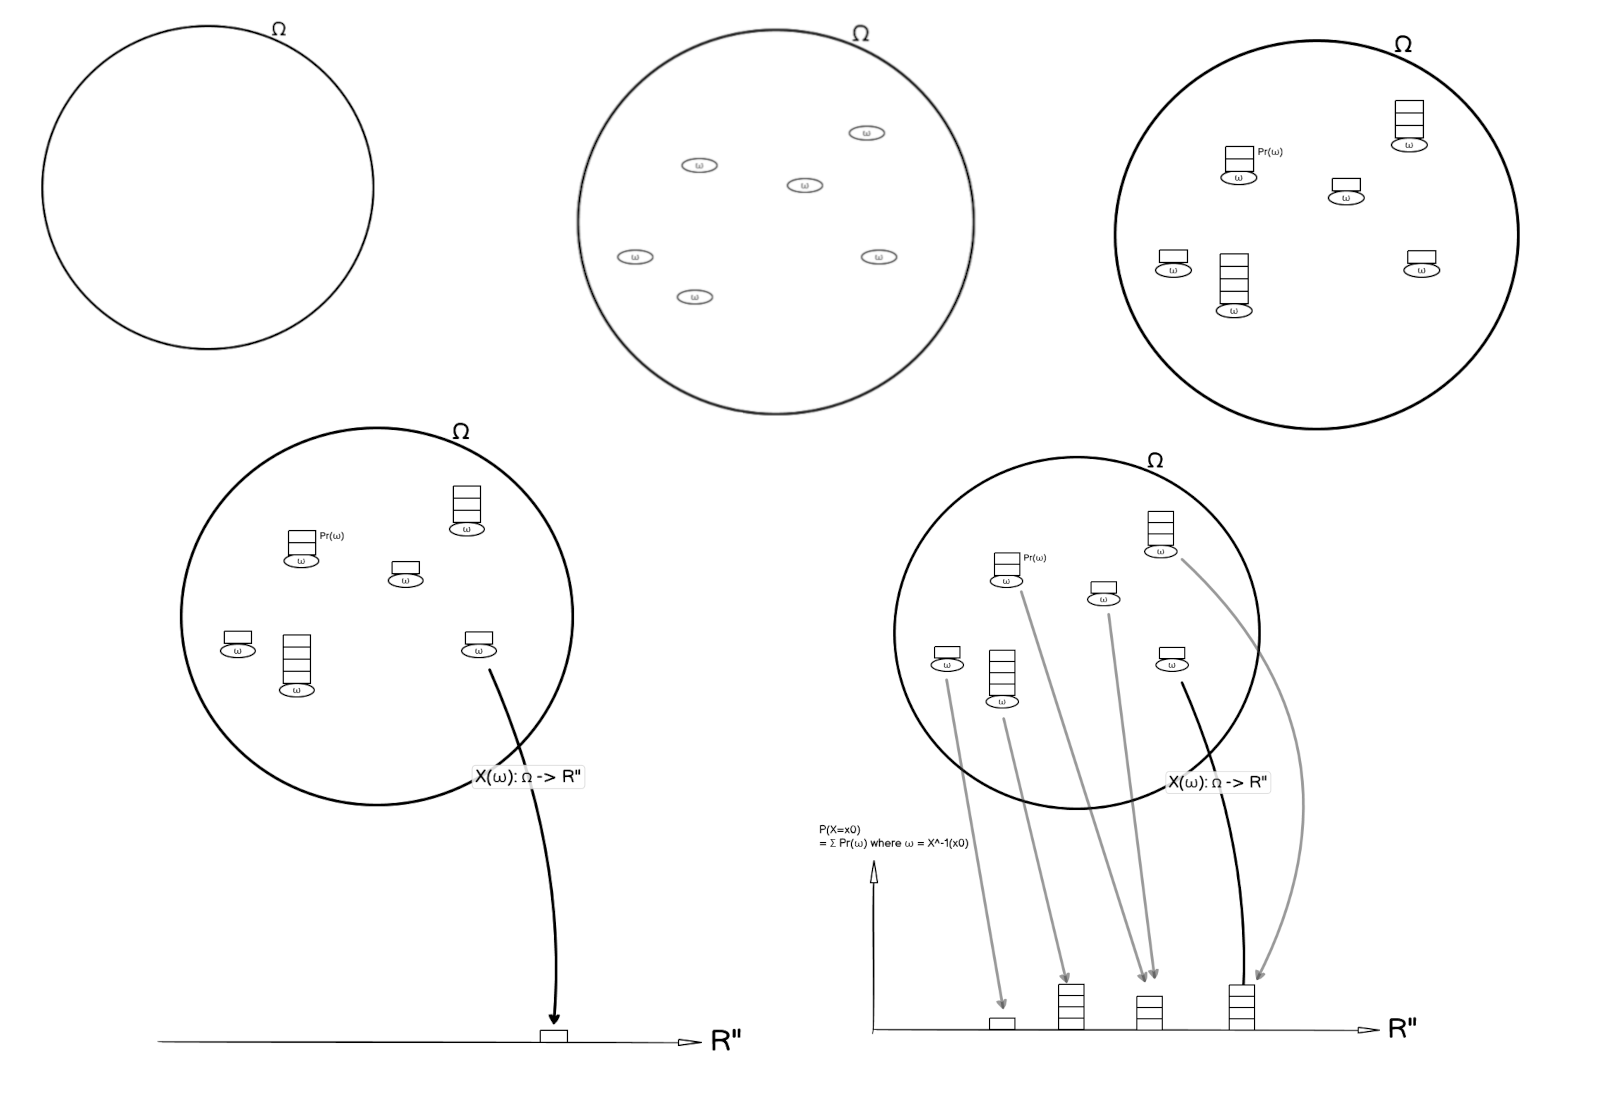
\includegraphics[width=0.85\textwidth]{images/prob.png}
\end{figure}


\begin{definition}[Expectation]
    The expectation of a random variable is defined as 
    $$ E[X] = \sum_\samplespace X(\omega)P(\omega)$$ 
\end{definition}

\begin{definition}[Conditional Probability]
    $$ \probFunct[A | B] = \frac{\probFunct[A \intersection B]}{\probFunct[B]}$$
\end{definition}

As a nice little exercise, we prove the formula for the conditional probability of the \emph{complement} of $B$.

\begin{proof}
    $$ \probFunct[A | \overline{B}] = $$
\end{proof}



As an illustrative example, consider the following probabilities. People can be \emph{small} (S) or \emph{tall} (T). They can be \emph{good} (G) or \emph{bad} (B) at basketball.
Here are the tables of probabilities:

\begin{table}[H]
    \centering
    \begin{tabular}{llllll}
      &      &  &   & S    & T    \\
      &      &  &   & 0.6  & 0.4  \\
      &      &  &   &      &      \\
      &      &  &   & S    & T    \\
    B & 0.14 &  & B & 0.54 & 0.08 \\
    G & 0.86 &  & G & 0.6  & 0.32
    \end{tabular}
\end{table}

\begin{table}[H]
    \centering
    \begin{tabular}{llll}
        $P(B|S)$ & 0.9 & $P(B|T)$ & 0.8 \\
        $P(G|S)$ & 0.1 & $P(G|T)$ & 0.2 
    \end{tabular}
\end{table}

Notice the following facts:
\begin{itemize}
    \item notice how $P(G|T) \neq 1 - P(G|S)$
    \item notice how $P(G|T) = 1 - P(B|T)$
    \item $P(A, B) = P(A|B) P(B) = P(B|A) P(A)$
    \item $ \Sigma_A \Sigma_B P(A, B) = 1.0 $
\end{itemize}

As yet another exercise, here is the formula of the probability of a union of arbitrary events: 

\begin{proof}
    $$ \probFunct (\union A_i) = \sum_i \probFunct(A_i) 
            - \sum_i \sum_{j>i} \probFunct(A_i \intersection A_j) 
            + \sum_i \sum_{j>i} \sum_{k>j} \probFunct(A_i \intersection A_j \intersection A_k) 
            - ...  $$
    
    This is proven by induction. 
                
    \subprf{Base case:}{$\probFunct(A_1 \union A_2) = \probFunct(A_1) + \probFunct(A_2) - \probFunct(A_1 \intersection A_2) $}{
        This is tirivally true when looking at a Venn Diagramm. 
    }
    \subprf{Induction step. Suppose that... }{ }{
    }
    
    
\end{proof}

\subsubsection{A few lemmas on conditional probability} \label{condPropLemmas}

In a "causal" chain of events $A, B, C$ we can integrate out the middle-event $B$.
\begin{equation}
    \begin{aligned}
        p(A, B, C)  &= \frac{p(A, B, C)}{p(A, B)} \frac{p(A, B)}{p(A)} p(A) \\
                    &= p(C|AB) p(B|A) p(A) \\
    \end{aligned}
\end{equation}

\begin{equation}
    p(A, C) = \Sigma_B p(A, B, C)
\end{equation}

\begin{equation}
    \begin{aligned}
            p(C | A) &= \frac{p(A, C)}{p(A)} \\
                     &= \Sigma_B p(C|A, B) p(B|A)
    \end{aligned}
\end{equation}

We can take the expression for conditional probability and condition \emph{every term} on a third event.
\begin{equation}
    \begin{aligned}
        p(B|A, C) &= \frac{p(A, B, C)}{p(A, C)} \\
        p(A|B, C) &= \frac{p(A, B, C)}{p(B, C)} \\
        p(A|B, C) &= \frac{p(B|A, C) p(A|C) p(C)}{p(B|C)p(C)} \\
                  &= \frac{p(B|A, C) p(A|C)}{p(B|C)} \\
    \end{aligned}
\end{equation}


\subsection{Decomposing variance - the road to sensitivity analysis}

\paragraph{Expressing variance as expectation} ...
\begin{equation}
    \begin{aligned}
        V_X &= E_{ (X - E_X)^2 } \\
            &= E_{ X^2 - 2 X E_X + E_X^2 } \\
            &= E_{X^2} - E_X^2
    \end{aligned}
\end{equation}

\paragraph{Conditional expectation and variance} ...

\begin{definition} \label{conditionalExpectation}
    Conditional expectation:
    $$ E_{Y|x} = \Sigma y P(y|x) $$
\end{definition}

\begin{definition} \label{conditionalVariance}
    Conditional variance: 
    $$ V_{Y|x} = E_{(Y - E_{Y|x})^2 | x} $$ 
\end{definition}

\paragraph{Law of total expectation} ...
\begin{equation} \label{lawOfTotalExpectation}
    \begin{aligned}
        E_Y &= \Sigma_Y y P(y) \\
            &= \Sigma_Y y \Sigma_X P(y|x) P(x) \\
            &= \Sigma_X (\Sigma_Y y P(y|x)) P(x) \\
            &= \Sigma_X E_{Y|x} P(x) \\
            &= E_{E_{Y|x}}
    \end{aligned}
\end{equation}

\paragraph{Law of total variance} ...
\begin{equation} \label{lawOfTotalVariance}
    \begin{aligned}
        V_Y &= E_{Y^2} - E_Y^2 \\
            &= E_{E_{Y^2 | X}} - E^2_{E_{Y|X}} \\
            &= E_{  V_{Y|X} + E^2_{Y|X}  } - E^2_{E_{Y|X}} \\
            &= E_{V_{Y|X}} + E_{E^2_{Y|X}} - E^2_{E_{Y|X}} \\
            &= E_{V_{Y|X}} + V_{E_{Y|X}}
    \end{aligned}
\end{equation}


\begin{figure}[h]
    \caption{Illustration of the law of total variance}
    \centering
      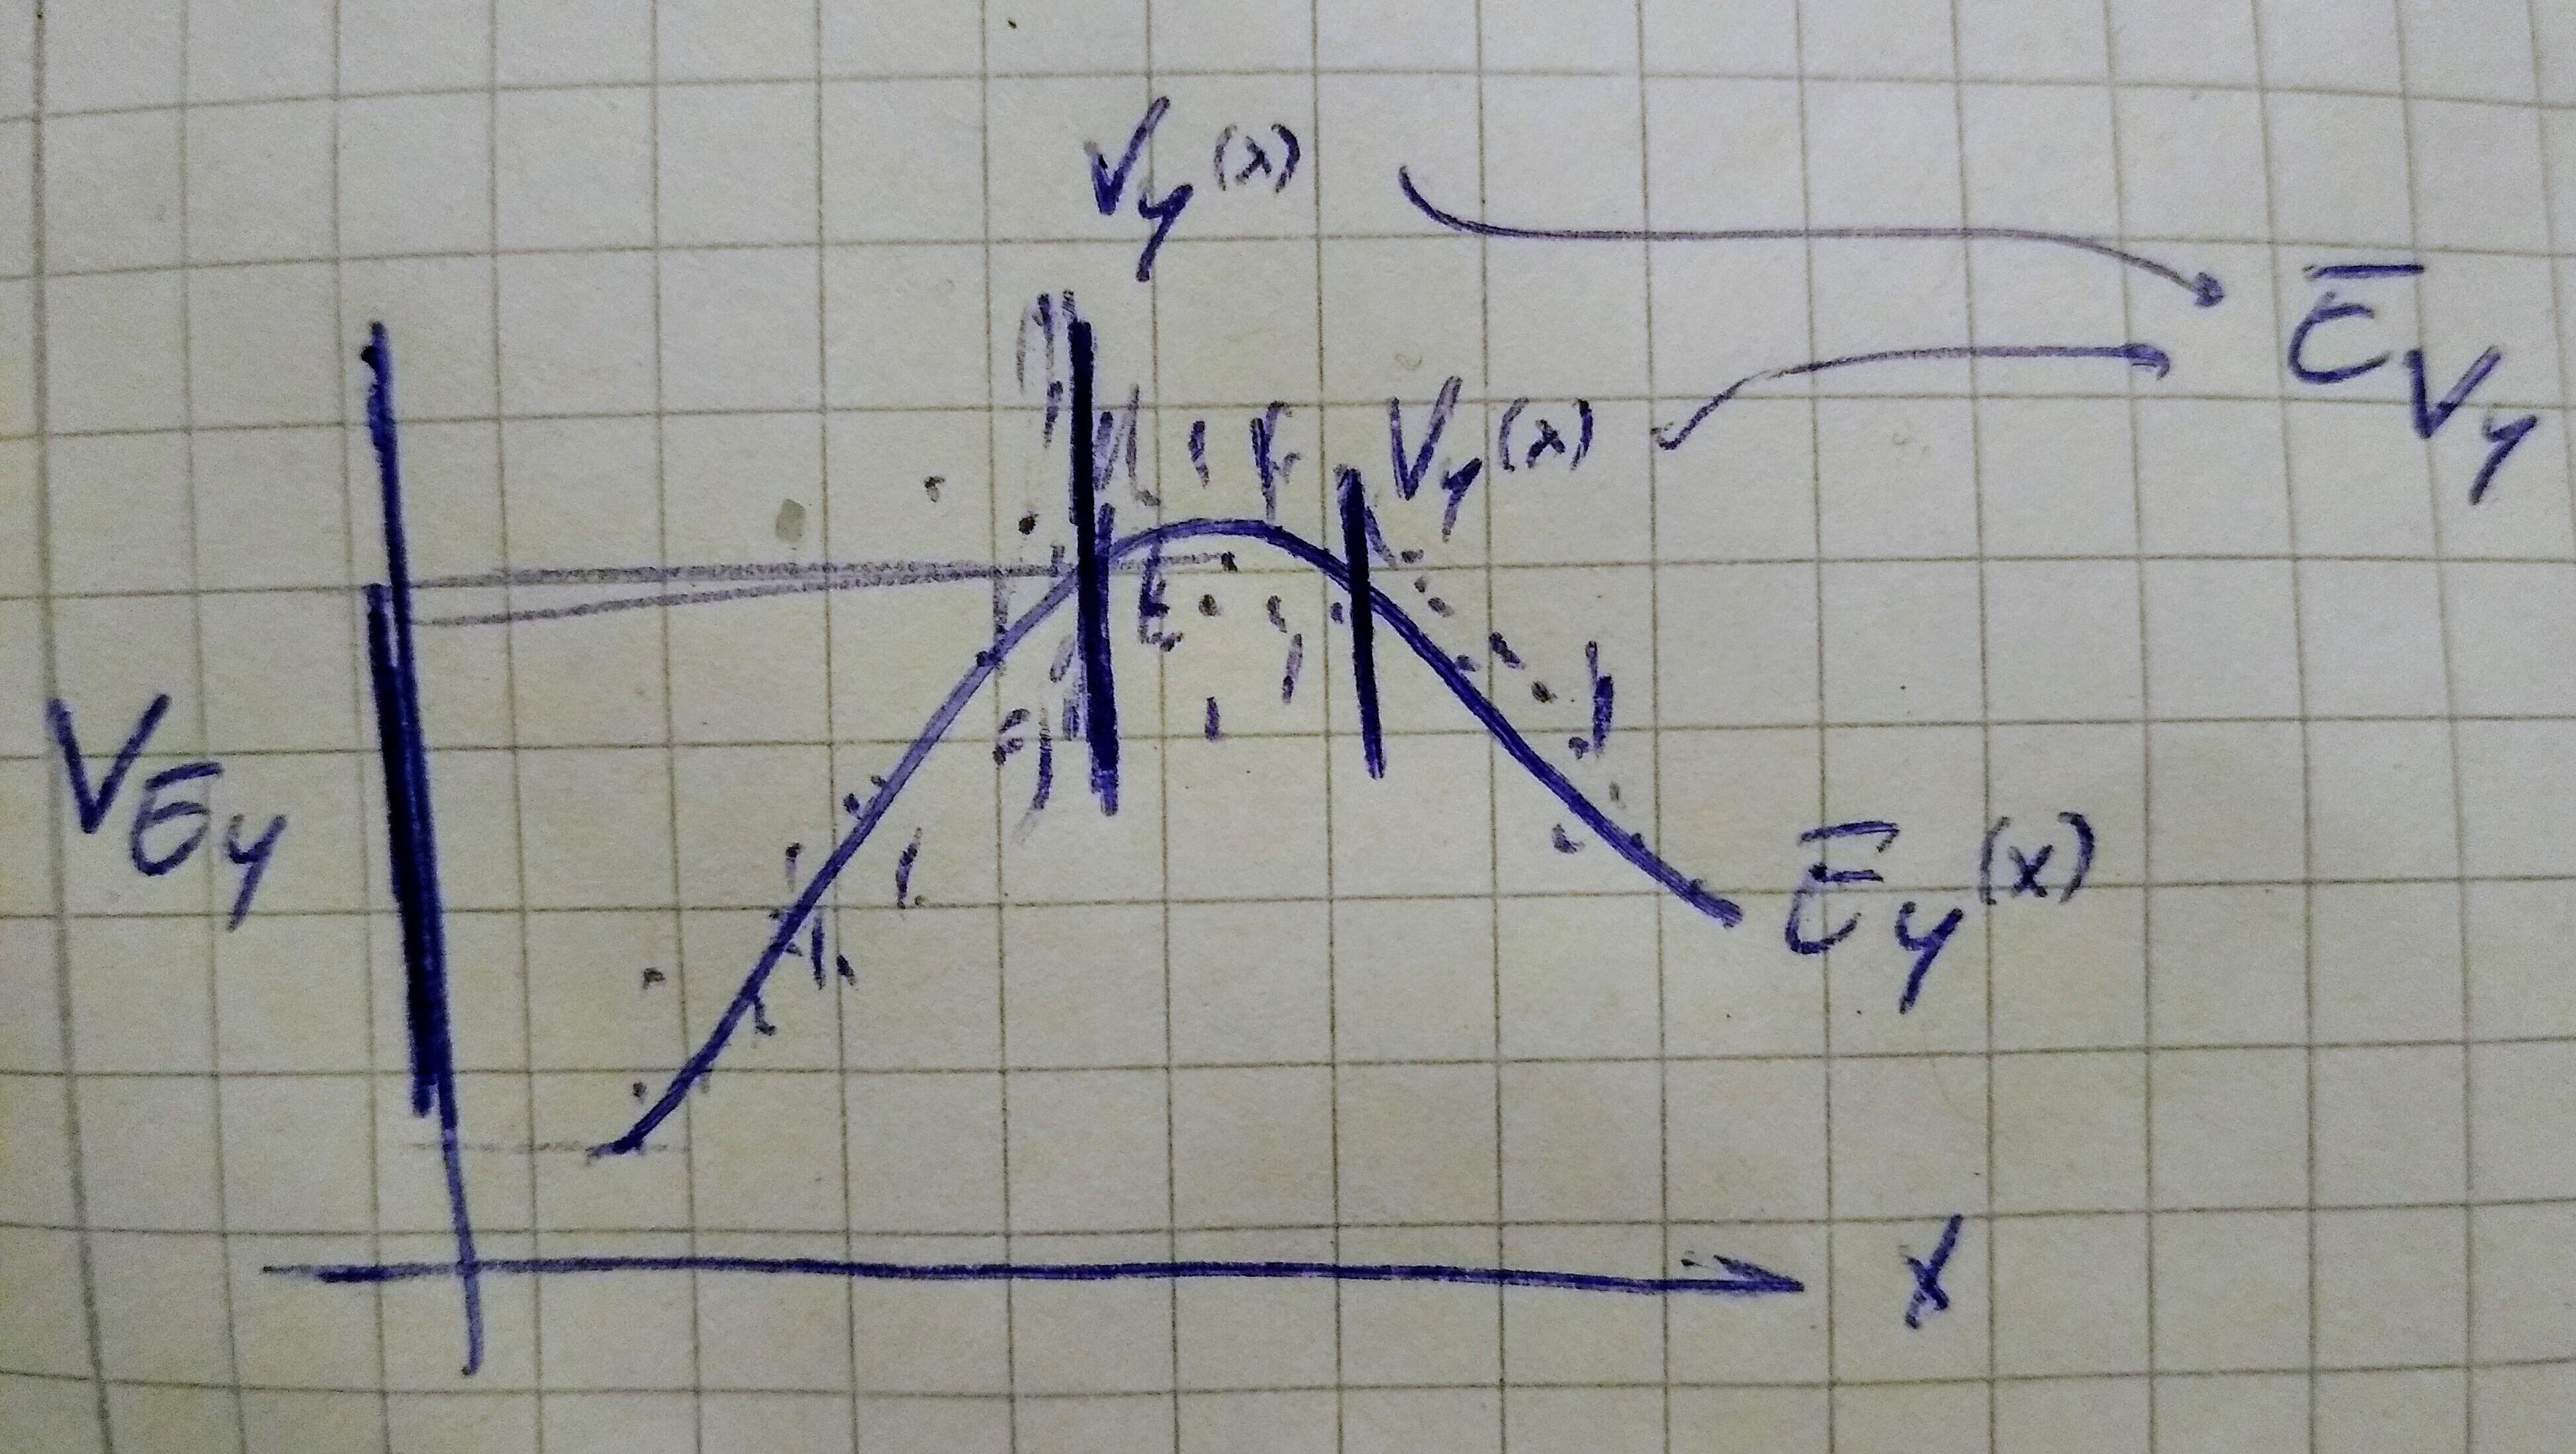
\includegraphics[width=0.5\textwidth]{images/law_of_total_variance.jpg}
\end{figure}
 
 
\subsection{Probability density functions}
Up to now we have been dealing with probability mass functions on discrete variables.
That works just as well with discrete variables, but we need to accommodate some details.
For example, we can only define probability density in therms of cumulative probability functions.

Let $P(x) := Pr(X > x)$ be a cumulative probability function.
Then the probability density at $x$ is $\frac{d P}{d x}(x)$.

\paragraph{As an exercise,} consider $x \tilde Exp(x)$. We want to calculate $E(x | x > x_0)$. 
We'll start with $P(x | x > x_0)$.
We have:
\begin{equation}
    \begin{aligned}
        P(X | X > x_0) &= \left( \text{ using the fact that } P(B|A) = \frac{P(A \land B)}{P(A)} \right) \\
                          &= \frac{ P(X = x \land X > x_0) }{ P(X > x_0) } \\
                          &= \frac{ s_{x_0} P(X=x) }{ P(x > x_0) }  (\text{ with $s_{x_0}$ the step-function at $x_0$}) \\
                          &= \frac{ s_{x_0} P(X=x) }{ \int_{x_0}^\infty p(x) dx }
    \end{aligned}
\end{equation}

This leads us to the expectation:

\begin{equation}
    \begin{aligned}
        E(X | X > x_0)  &= \int_{-\infty}^\infty x p(X | X > x_0) dx \\
                        &= \frac{ s_{x_0} \int_{-\infty}^\infty x p(x) dx }{ \int_{x_0}^\infty p(x) dx } \\
                        &= \frac{ \int_{x_0}^\infty x p(x) dx }{ \int_{x_0}^\infty p(x) dx } \\
                        &= \frac{ s_{x_0} E(X) }{ P(X > x_0) } 
    \end{aligned}
\end{equation}


\subsection{Probability distributions}

A probability distribution is a function from the domain of a random variable to its probability - in other words, a probability distribution yields the probability that a random variable will take on a certain value. 

There is an abundance of ready made probability distributions to chose from, covering virtually all important situations. But care must be taken when deciding which distribution to apply to a certain problem. 

\paragraph{The Bernoulli family} based on modelling a series of coin-tosses.
\begin{itemize}
    \item Bernoulli: heads or tails?
    \item Binominal: k heads in n trials
    \item Poisson: k heads in $\infty$ trials. 
\end{itemize}
A remarkable feature of the Poisson-distribution is that it has only a parameter for the mean, but always the same variance.

\paragraph{The geometric family} based on repeating an experiment until it succeeds. 



\subsubsection{Probabilistic fallacies}
\begin{itemize}
    \item T-Test interpretation: If $\probFunct[A|B] = x$, then this does \emph{not} mean that $\probFunct[A|\overline{B}] = 1 - x$.
    \item Prosecutors fallacy aka. inverse fallacy: $P(A|B) \neq P(B|A)$
\end{itemize}

\paragraph{$\probFunct[A|\overline{B}] \neq 1 - \probFunct[A | B]$}. 
\begin{proof}
    By contradiction. 
    \begin{equation}
        \begin{aligned}
           \probFunct[A|B]                 &= 1 - \probFunct[A | \overline{B}] \\
                                           &= \frac{  \probFunct[B] - \probFunct[A \intersection \overline{B}]  }{  \probFunct[B]  }  \\
           \probFunct[A|B] \probFunct[B]   &=         \probFunct[B] - \probFunct[A \intersection \overline{B}] \\
           \probFunct[A \intersection B]   &= \probFunct[B] - \probFunct[A \intersection \overline{B}] \\
           \probFunct[A \intersection B] + \probFunct[A \intersection \overline{B}]  &= \probFunct[B] \\
           \probFunct[A] &= \probFunct[B]
        \end{aligned}
    \end{equation}
    Thus $\probFunct[A|\overline{B}] \neq 1 - \probFunct[A | B]$. But not that it \emph{does} hold true that $\probFunct[\overline{A}|B] = 1 - \probFunct[A | B]$
\end{proof}


\section{Statistics}

\subsection{Correlation}
Assume an inner product space.

\subsection{Linear regression}

Assume that reality can me modelled by a model like this one: 

$$ \vec{y} = \mtrx{X} \vec{w} + \vec{e} $$

Not knowing $\vec{e}$, our best guess at the outcome would be 

$$ \vec{\hat{y}} = \mtrx{X} \vec{w} $$

We can find the gradient of w by:

$$ \partDiff{E}{\vec{w}} = -  (\vec{y} - \vec{\hat{y}}) \mtrx{X}  $$



\subsection{Spatial modelling}

\subsubsection{Generalized least squares}
like linear regression, but errors are not iid, but allowed to be correlated.

\subsubsection{Gaussian processes}
Gaussian processes are a means of interpolating a value $y_x$ from surrounding values $y_x = \sum \alpha_i y_i$. Basic intuition from \href{https://bookdown.org/rbg/surrogates/chap5.html}{here}.
That is different from what linear regression or its extension GLS do: regression predicts $y$ from explanatory variables $x$, assuming a (linear) model.
Gaussian processes don't do that. They only interpolate between already observed $y$'s. No model is assumed.

Consider the $n \times m$ surface $\mtrx{Y}$. Assume that the value of any pixel in $\mtrx{Y}$ follows a gaussian distribution - which may be correlated to all other pixels in $\mtrx{Y}$.
Millions of surfaces $\mtrx{Y}$ may be sampled from $N(\vec{0}, \mtrx{\Sigma}) = P(\mtrx{Y})$, where $\vec(0)$ is of size $n \times m$ and $\mtrx{\Sigma}$ is of size $nm \times nm$.
We call $P(\mtrx{Y})$ the prior. $\mtrx{\Sigma}$ can be very large, so we assume that it can be modeled by a covariance-function $cov(h)$ which is \emph{only dependent on the distance between two points, not on the points themselves}.

\begin{lstlisting}[language=python]
import numpy as np
import matplotlib.pyplot as plt
from scipy.stats import multivariate_normal

def size(x):
    return np.sqrt(np.sum(np.power(x, 2)))

def distance(x0, x1):
    return size(x0 - x1)

def getDistanceMatrix(rowPoints, colPoints):
    # deliberately not exploiting symmetry 
    # <- this way it works with non-square matrices, too.
    rows = len(rowPoints)
    cols = len(colPoints)
    distances = np.zeros((rows, cols))
    for i in range(rows):
        for j in range(cols): 
            p0 = rowPoints[i]
            p1 = colPoints[j]
            d = distance(p0, p1)
            distances[i, j] = d
    return distances

deltaX = 0.1
deltaY = 0.1
gridX = 20
gridY = 20
nrPoints = gridX * gridY
points = np.zeros((nrPoints, 2))
for x in range(gridX):
    for y in range(gridY):
        i = x * gridX + y
        points[i] = [x * deltaX, y * deltaY]
distances = getDistanceMatrix(points, points)

mean = np.zeros((nrPoints))
cov0 = 1.3  # overall variance
h95 = 2     # distance at which cov(h) >= 0.95 * cov0

def variogramFunction(h):
    return cov0 * ( 1 - np.exp( -3*h/h95 ) )

Sigma = cov0 - variogramFunction(distances)
prior = multivariate_normal(mean, Sigma)

sample1 = prior.rvs()
sample2 = prior.rvs()
sample3 = prior.rvs()
\end{lstlisting}

\begin{figure}[H]
    \caption{3 samples from prior $P(\mtrx{Y})$}
    \centering
    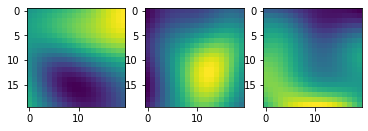
\includegraphics[width=0.7\linewidth]{images/gp_prior_samples.png}
\end{figure}

We have observed some samples $\mtrx{D} = {(x_i, y_i)}$.
Which of these millions of surfaces are most likely given those observations? We can answer that with $P(\mtrx{Y}|\mtrx{D})$.
\begin{figure}[H]
    \caption{Observations $\mtrx{D}$. Which field $\mtrx{Y}$ is most likely to have produced these observations?}
    \centering
    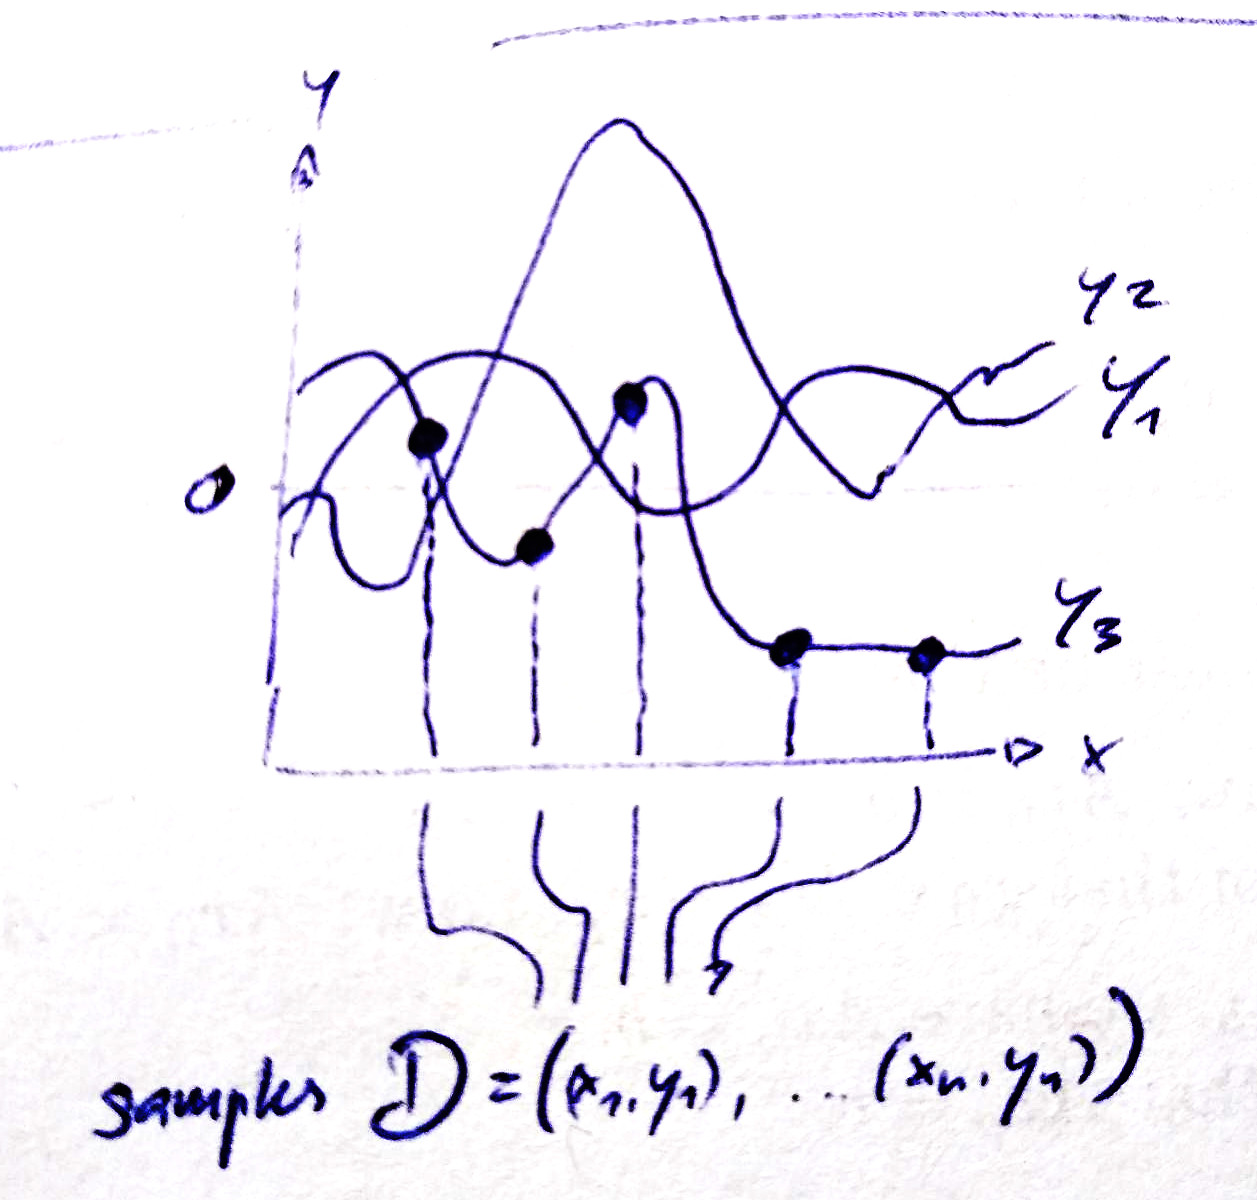
\includegraphics[width=0.4\linewidth]{images/gp_observations.jpg}
\end{figure}

We can calculate the posterior using 
$$
P(\mtrx{Y}|\mtrx{D}) \sim P(\mtrx{D}|\mtrx{Y}) P(\mtrx{Y})
$$
But since in gaussian processes we assume multivariate-normals, this can be done much easier.

Consider a multivariate normal distribution on, say, 400 dimensions $N(\vec{\mu}, \mtrx{\Sigma})$. Those 400 dimensions could, for example, be pixel-values in a 20 by 20 image.
Now assume that out of those 400 dimensions we have measurements for $s$ samples, leaving a rest $r = 400 - s$.
For multivariate-normal distributions, we can easily and analytically obtain the conditional distribution $P(\vec{y}_r | \vec{y}_s) = N(\hat{\vec{\mu}}, \hat{\mtrx{\Sigma}})$.

Split $\vec{y}$ like so:
$$ y = \myarray{\vec{y}_r \\ \vec{y}_s} $$
Analogously we can split the covariance-matrix:
$$ \mtrx{\Sigma} = \begin{bmatrix}
    \mtrx{\Sigma}_{rr} & \mtrx{\Sigma}_{rs} \\
    \mtrx{\Sigma}_{sr} & \mtrx{\Sigma}_{ss} \\
\end{bmatrix}  $$

Then, according to \href{https://en.wikipedia.org/wiki/Multivariate_normal_distribution#Conditional_distributions}{wikipedia}, we can obtain $\hat{\vec{\mu}}$ and $\hat{\mtrx{\Sigma}}$ like so:
$$ \hat{\vec{\mu}}_r = \vec{\mu}_r + \mtrx{\Sigma}_{rs} \mtrx{\Sigma}_{ss}^{-1} (\vec{y}_s - \vec{\mu}_s) $$
$$ \hat{\mtrx{\Sigma}}_r = \mtrx{\Sigma}_{rr} - \mtrx{\Sigma}_{rs} \mtrx{\Sigma}_{ss}^{-1} \mtrx{\Sigma}_{sr} $$

\begin{lstlisting}[language=python]
indices = np.arange(nrPoints)
sampleIndices = np.asarray(list(
    map(lambda x: int(x),
        samples[:, 0])))
nonSampleIndices = np.asarray(list(
    filter(lambda v: v not in sampleIndices,
           indices)))
samplePoints = points[sampleIndices]
nonSamplePoints = points[nonSampleIndices]
sampleValues = samples[:, 3]

# For simplicity, we just re-calculate SigmaXX here.
# But we could have also picked the right values from Sigma
# without any need for re-computation.
distancesRR = getDistanceMatrix(nonSamplePoints, nonSamplePoints)
SigmaRR = cov0 - variogramFunction(distancesRR)

distancesSS = getDistanceMatrix(samplePoints, samplePoints)
SigmaSS = cov0 - variogramFunction(distancesSS)
SigmaSSInverse = np.linalg.inv(SigmaSS)

distancesRS = getDistanceMatrix(nonSamplePoints, samplePoints)
SigmaRS = cov0 - variogramFunction(distancesRS)
SigmaSR = SigmaRS.transpose()

meanPosterior = SigmaRS @ SigmaSSInverse @ sampleValues
SigmaPosterior = SigmaRR - SigmaRS @ SigmaSSInverse @ SigmaSR

posterior = multivariate_normal(meanPosterior, SigmaPosterior)   
\end{lstlisting}

We can now plot the \inlinecode{meanPosterior} around our \inlinecode{samples}. Doing so we obtain the graphic as shown in figure \ref{gpPosterior}.

\begin{figure}[H]
  \centering
  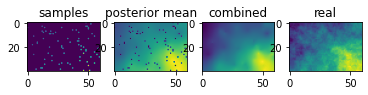
\includegraphics[width=0.7\linewidth]{images/gp_posterior_samples.png}
  \caption{Samples and fitted posterior fit together well}
  \label{gpPosterior}
\end{figure}


Note how we assumed that the covariance matrix $\mtrx{\Sigma}$ could be parameterized with a covariance-function $c(h)$. Only this way do we have any chance of finding a good approximation for $\mtrx{\Sigma}$ with only few samples.
The relation \inlinecode{Sigma = cov0 - variogramFunction(distances)} comes from the variogram $\gamma(h)$ as in here:
\begin{equation}
  \begin{aligned}
    2 \gamma(h) &= E[(Z(x+h) - Z(x))^2] \\
                &= E[( (Z(x+h) - \mu) - (Z(x) - \mu) )^2] \\
                &= E[ (Z(x+h) - \mu)^2  - 2(Z(x+h) - \mu)(Z(x) - \mu)  + (Z(x) - \mu)^2 ] \\
                &= E[ (Z(x+h) - \mu)^2 ]  - 2 E[(Z(x+h) - \mu)(Z(x) - \mu)]  + E[ (Z(x) - \mu)^2 ] \\
                &= c(0) - 2 c(h) + c(0) \\
      \gamma(h) &= c(0) - c(h) \\
           c(h) &= c(0) - \gamma(h)
  \end{aligned}
\end{equation}
In practical applications, we'll usually fit our function \inlinecode{cov0 * ( 1 - np.exp( -3*h/h95 ) )} by moving the parameters \inlinecode{cov0} and \inlinecode{h95} until the residuals fit properly.
Our code would then look like this:

\begin{lstlisting}[language=python]
def empiricalVariogram(distanceMatrix, data):
  variogram = {}
  d0 = np.min(distanceMatrix)
  d1 = np.max(distanceMatrix)
  nrHs = 20
  deltaH = (d1 - d0) / nrHs
  for h in np.linspace(d0, d1, nrHs):
      Nh = 0
      hSum = 0
      pairs = (h <= distanceMatrix) * (distanceMatrix < h+deltaH)
      for i in range(nrTotal):
          for j in range(i, nrTotal):
              if pairs[i, j]:
                  v = data[i]
                  vh = data[j]
                  hSum += np.power(v - vh, 2)
                  Nh += 1
      if Nh > 0:
          variogram[h] = hSum / (2 * Nh)
    return variogram
    
def fitVariogram(samples):
    pass  # TBD


residuals = prediction - samples
(cov0, h95) = fitVariogram(residuals)

SigmaRR = cov0 - variogramFunction(cov0, h95, distancesRR)
SigmaSS = cov0 - variogramFunction(cov0, h95, distancesSS)
SigmaRS = cov0 - variogramFunction(cov0, h95, distancesRS)
SigmaSR = SigmaRS.transpose()
SigmaSSInverse = np.linalg.inv(SigmaSS)

meanPosterior = prediction + SigmaRS @ SigmaSSInverse @ sampleValues
SigmaPosterior = SigmaRR - SigmaRS @ SigmaSSInverse @ SigmaSR

predictionPosterior = meanPosterior
\end{lstlisting}


For more, see this \href{https://michaeloneill.github.io/GPR-tutorial.html}{very thorough tutorial}.

\subsubsection{AR and SAR}
Autoregressive and spatial-autoregressive models.

\subsubsection{Comparison}

\begin{table}[H]
    \centering
    \resizebox{\textwidth}{!}{%
    \begin{tabular}{@{}llll@{}}
    \toprule
     &
      Generalized least squares &
      Gaussian processes &
      AR \\ \midrule
    \multicolumn{1}{|l|}{type} &
      \multicolumn{1}{l|}{\begin{tabular}[c]{@{}l@{}}Predict y from x.\\ Has explanatory variables.\end{tabular}} &
      \multicolumn{1}{l|}{\begin{tabular}[c]{@{}l@{}}Interpolate y from other y's.\\ Explanatories can be added with GLS\end{tabular}} &
      \multicolumn{1}{l|}{interpolate y from other y's} \\ \midrule
    \multicolumn{1}{|l|}{model} &
      \multicolumn{1}{l|}{\begin{tabular}[c]{@{}l@{}}$y = X\alpha + \epsilon$\\ \\ $\epsilon \sim N(\vec{0}, \mtrx{\Sigma})$\end{tabular}} &
      \multicolumn{1}{l|}{\begin{tabular}[c]{@{}l@{}}$Y \sim N(\vec{0}, \mtrx{\Sigma})$\\ $P(\mtrx{Y}|\mtrx{D}) = N(\hat{\vec{\mu}}, \hat{\mtrx{\Sigma}})$\\ $\tilde{y} = \sum \alpha_i \vec{y}_i$\\ Y is a field of size n by m\\ D is the observations \end{tabular}} &
      \multicolumn{1}{l|}{\begin{tabular}[c]{@{}l@{}}$y_t = \sum \alpha_i y_{t-i} + \epsilon$\\ $\epsilon \sim N(0, \sigma)$, iid \end{tabular}} \\ \midrule
    \multicolumn{1}{|l|}{Specialities} &
      \multicolumn{1}{l|}{} &
      \multicolumn{1}{l|}{\begin{tabular}[c]{@{}l@{}}$\mtrx{\Sigma}$ is encoded using a covariance-function cov(h)\\ to save on parameters\end{tabular}} &
      \multicolumn{1}{l|}{} \\ \midrule
    \multicolumn{1}{|l|}{$\epsilon$} &
      \multicolumn{1}{l|}{} &
      \multicolumn{1}{l|}{} &
      \multicolumn{1}{l|}{} \\ \midrule
    \multicolumn{1}{|l|}{$cov(\epsilon_i, \epsilon_j)$} &
      \multicolumn{1}{l|}{} &
      \multicolumn{1}{l|}{} &
      \multicolumn{1}{l|}{} \\ \midrule
    \multicolumn{1}{l|}{$cov(y_i, y_j)$} &
      \multicolumn{1}{l|}{} &
      \multicolumn{1}{l|}{} &
      \multicolumn{1}{l|}{} \\ \bottomrule
    \end{tabular}%
    }
    \end{table}


\subsection{Bayesian networks}
Bayesian networks are a neat tool when we can manually encode some complex causation-graphs.

\begin{lstlisting}[language=python]

  def find(lst, predicate):
  for entry in lst:
      if predicate(entry):
          return entry

def prod(lst):
  p = lst[0]
  for entry in lst[1:]:
      p *= entry
  return p

def getCombinations(lists):
  combinations = []
  if len(lists) == 0:
      combinations = []
  elif len(lists) == 1:
      combinations = lists[0]
  elif len(lists) == 2:
      for a in lists[0]:
          for b in lists[1]:
              combinations.append([a, b])
  else:
      firstList = lists[0]
      subCombos = getCombinations(lists[1:])
      for a in firstList:
          for b in subCombos:
              combinations.append([a, *b])
  return combinations



class Node:
  def __init__(self, name, pmf, allowedValues, parents = []):
      self.name = name
      self.pmf = pmf
      self.allowedValues = allowedValues
      self.parents = parents

  def setPmf(self, pmf):
      self.pmf = pmf

  def calcProb(self, value):

      if value not in self.allowedValues:
          return 0.0

      parentData = self.__getParentData()
      
      p = 0.0
      if len(parentData) > 0:
          for combination in getCombinations(parentData):
              parentValues = {entry['name']: entry['value'] for entry in combination}
              parentProbs = [entry['prob'] for entry in combination]
              p += self.pmf(value, parentValues) * prod(parentProbs)
      else:
          p = self.pmf(value, {})

      return p

  def __getParentData(self):
      parentData = []
      for i, parent in enumerate(self.parents):
          parentData.append([])
          for value in parent.allowedValues:
              prob = parent.calcProb(value)
              parentData[i].append({
                  'name': parent.name,
                  'value': value,
                  'prob': prob
              })
      return parentData


class Net:
  def __init__(self, nodes):
      self.nodes = nodes
      self.memo = {}
      for node in self.nodes:
          self.memo[node.name] = {}

  def calcProb(self, nodeName, value):
      if self.memo[nodeName][value]:
          return self.memo[nodeName][value]
      else:
          node = self.__findNode(nodeName)
          prob = node.calcProb(value)
          self.memo[nodeName][value] = prob
          return prob

  def setPmf(self, nodeName, pmf):
      # setting pmf
      node = self.__findNode(nodeName)
      node.setPmf(pmf)

      # invalidating downstream cached results
      self.memo[nodeName] = {}
      children = self.__findChildren(nodeName, True)
      for child in children:
          self.memo[child.name] = {}

  def __findNode(self, nodeName):
      node = find(self.nodes, lambda n: n.name == nodeName)
      return node

  def __findChildren(self, nodeName, recursive=False):
      pass



def randomSelection(door, parents):
  return 1/3

guest = Node('guest', randomSelection, [1, 2, 3])

real = Node('real', randomSelection, [1, 2, 3])


def pickingRandomOther(door, parents):
  if parents['real'] == door:
      return 0
  if parents['guest'] == door:
      return 0
  elif parents['real'] == parents['guest']:
      return 1/2
  else:
      return 1

monty = Node('monty', pickingRandomOther, [1, 2, 3], [real, guest])


# %%
monty.calcProb(1)
# %%
def guestPicked1(door, parents):
  if door == 1:
      return 1
  else:
      return 0

guest.setPmf(guestPicked1)

monty.calcProb(2)
# %%
def realDoorIs2(door, parents):
  if door == 2:
      return 1
  else:
      return 0

real.setPmf(realDoorIs2)

monty.calcProb(3)
\end{lstlisting}






\subsection{Tests}
Often, statistical tests work \emph{the wrong way round}. You have your hypothesis, like "these groups are different". Then you state the opposite, the \emph{null-hypothesis}. Then you determine how likely your data is under the null-hypothesis - the \emph{p-value}. And than you hope that the p-value is very low.

\paragraph{Students T-Test} compares two averages (means) and tells you if they are different from each other. The null hypothesis is that all samples come from the same distribution. That means that under $H_0$, the two means you obtained should be similar. So the interpretation goes like this: 
\begin{itemize}
    \item low p-value: the chance that your result would have happend under $H_0$ is low. It is very unlikely that the two means you have obtained actually come from the same distribution. 
    \item high p-value: It is quite possible that both your groups come from the same distribution. 
\end{itemize}
Note that there are two experimental setups that can use t-tests:
\begin{itemize}
    \item unpaired: you have two groups, with no person in both groups. Example: Test one group with medication and another with placebo. 
    \item paired: every person is first in the first and then in the second group. Example: test patients before and after treatment. 
\end{itemize}

\section{Graph Theory}

\subsection{General properties}

\subsubsection{Degrees}

\begin{theorem} \label{sumIndegreesIsNrEdges}
    In a directed graph $\sum_{V_G} \indeg(v_n) = |E_G|$
\end{theorem}

\begin{proof}
    \induction{$ \sum_{V_G} \indeg(v_n) = |E_G| $ \\}
    {$\sum_{V_G} \indeg(v_n) = |E_G|$ where $E_G = \{(v_1, v_2)\}$ \\}
    {This is tirvially true.}
    {
    \begin{itemize}
        \item Let $\sum_{V_G} \indeg(v_n) = |E_G|$ 
        \item Let $V_{G'} = V_G \cup \{v_{N+1}\}$
        \item Let $E_{G'} = E_G \cup \{(x, y) \in V_G \times \{v_{N+1}\} \cup \{v_{N+1}\} \times V_G \}$
    \end{itemize}
    }
    {
     For the left side it holds that: 
                $$ \sum_{V_{G'}} \indeg(v_n) = \sum_{V_G} \indeg(v_n) + \outdeg(v_{N+1}) + \indeg(v_{N+1}) $$
                On the other hand on the right side it holds that: 
                $$ |E_{G'}| = |E_G| + \outdeg(v_{N+1}) + \indeg(v_{N+1}) $$
                So the equation reduces to $0=0$, which is true.
    }
\end{proof}


\begin{lemma} \label{indegIsOutdeg}
    $\sum_{V_G} \indeg(v_n) = \sum_{V_G} \outdeg(v_n)$
\end{lemma}

\begin{lemma}
    In an undirected graph we have $\sum_{V_G} \degr(v_n) = 2|E_G|$
\end{lemma}

\subsection{Walks and paths}

\begin{definition}
    A walk is any sequence of vertices that are connected by an edge.
\end{definition}

\begin{definition}
    A path is a walk where no vertex appears twice.
\end{definition}

\begin{theorem}
    The shortest walk between any two vertices in a graph is a path.
\end{theorem}

\begin{proof}
    \subprf{By contradiction. Suppose that the vertex $x$ appears twice in the shortest walk.}{this is a contradiction.}{
        Since $x$ appears twice, the proposed walk must be of the form $f-x-g-x-h$, where $g$ is a sequence of $0$ or more connected vertices. Then this walk can be shortened to $f-x-h$.
    }
\end{proof}

\begin{theorem}
    The longest path in a graph has length $ | V_G | - 1 $.
\end{theorem}
This is too trivial for a full-fledged proof: there are no repetitions in a path, so it can only have as many steps as it has vertices.


\subsubsection{Relations and adjacency matrices}

Let $R \circ Q$ be a composition of two relations. The number of paths of length exactly $n$ between two vertices $x$ and $y$, written as $\paths_n(x, z)$, can be expressed  as 
 $$ \paths_n(x,z) = | \{ y | xRy \land yQz \} | = \sum_{y \in Y} xRy \cdot yQz$$


If $R_{AM}$ and $Q_{AM}$ are the adjacency matrix representations of the above relations, then: 

$$  R_{AM} \cdot Q_{AM} [n,m] = \sum_{y \in Y} R_{AM} [x_n, y] \cdot Q_{AM} [y, z_m] $$

$$ = \sum_{y \in Y} xRy \cdot yQz = \paths_n(x,z) $$

When $R=Q$, it follows easily that:

\begin{theorem}
    $R_{AM}^2 [n,m]$ is the number of paths  that go from $v_n$ to $v_m$ in exactly $2$ steps.
\end{theorem}

\begin{theorem} \label{all_possible_paths}
    $R_{AM}$ explains whether or not two vertices $v$ and $u$ are connected. All possible paths are listed in $R^* = R_{AM} \cup R_{AM}^2 \cup R_{AM}^3 \cup ... \cup R_{AM}^{|V_G|-1}$.
    We can find the length of the shortest path between two vertices $u$ and $v$ by
\end{theorem}



\subsection{Planar graphs}

The following theorems all deal with planar, connected graphs, and build up to Eulers theorem. Well use $N$ for the number of nodes, $E$ for the number of edges, and $L$ for the number of loops.

\begin{theorem}
    Adding a edge to a planar, connected graph means adding one loop: $ \Delta N = 0 \land \Delta E = 1 \then \Delta L = 1$
\end{theorem}

\begin{theorem}
    Adding x edges means adding x loops: $ \Delta N = 0 \land \Delta E = x \then \Delta L = x $
\end{theorem}

\begin{proof}
    \subprf{}{$\Delta N = 0 \land \Delta E = x \then \Delta L = x$}{
        By induction on $\Delta E$. \\
        \subprf{Base case: $\Delta E = 1$}{$\Delta L = 1$}{
            By theorem 11.
        }
        \subprf{Let $\Delta N = 0 \land \Delta E = x \then \Delta L = x$.\\}
            {$\Delta N = 0 \land \Delta E = x+1 \then \Delta L = x+1$}{
            Consider the graph from the induction hypothesis, then apply theorem 12.
        }
    }
\end{proof}

\begin{theorem}
    When we add a new node to a graph and connect it to the graph using one or more edges, then the number of edges and loops behaves as such: $ \Delta N = 1 \then \Delta L = \Delta E - 1 $
\end{theorem}

\begin{proof}
    \subprf{}{$\Delta N = 1 \then \Delta L = \Delta E - 1$}{
        Let $ \Delta N = 1 $. \\
        By induction on $ \Delta E $. \\
        \subprf{Base case: $\Delta E = 1 $}{$ \Delta L = 0 $}{
            Graphically trivial.
        }
        \subprf{Induction step: $\Delta L = \Delta E - 1$}{$\Delta L' = \Delta E' - 1$}{
            $\Delta E ' = \Delta E + 1$ \\
            Using theorem 12, that means:
            $\Delta L' = \Delta L +1$ \\
            Thus: 
            $\Delta L + 1 = \Delta E + 1 - 1 $ \\
            Which reduces to: 
            $\Delta L = \Delta E - 1$, which is true by the induction hypothesis.
        }
    }
\end{proof}

\begin{theorem}
    Eulers theorem: $N + L = E + 1$
\end{theorem}

\begin{proof}
    \subprf{}{$N + L = E + 1$}{
        By induction on $N$. \\
        \subprf{Base case: $N=1$ or $N=2$}{$N + L = E + 1$}{
            If $N=1$: $1 + 0 = 0 + 1$ \\
            If $N=2$: $2 + 0 = 1 + 1$
        }
        \subprf{Induction step: Let $N + L = E + 1$.\\}{$N+1 + L' = E' + 1$}{
            Using theorem 13: $\Delta L' = \Delta E - 1$ \\
            Thus:
            $N + 1 + L + \Delta L = E + \Delta E + 1$ \\
            $N + L = E + 1$, which is true  by the induction hypothesis.
        }
    }
\end{proof}



\subsubsection{Trees}


Here is a fun little proof.

\begin{proof} In a tree, the mean number of children ($mcc$) is always equal to $1 - 1/N$.
    
    \subprf{}{$mcc = 1 - \frac{1}{N}$}{
        With what we have so far, this is almost trivial to prove. 
        The mean child count can be written as 
        $$ mcc = \frac{1}{N} \sum_N \outdeg{v_n} $$
        Using theorem \ref{sumIndegreesIsNrEdges} and lemma \ref{indegIsOutdeg}, this becomes
        $$ mcc = \frac{1}{N} E $$
        Eulers formula in a tree becomes $N = E + 1$, since there are no loops in trees. Using this: 
        $$ mcc = 1 - \frac{1}{N} $$
    }

\end{proof}

When training a binary classifier, we usually need a measure of defining which of several trees is a good representation of the data. The number of nodes, however, cannot be used as a measure, because it is always going to be $2n - 1$.
\begin{proof} In a binary tree, the number of leaves $n$ equals $\frac{N+1}{2}$, regardless of the architecture of the tree.

    \subprf{}{$n = \frac{N+1}{2}$}{
        We shall use the fact that in any tree, $\sum_{V_G} \indeg(v_n) = \sum_{V_G} \outdeg(v_n)$. \\

        Consider the leaves of the tree. They all have $\indeg(v_n) = 1$ and $\outdeg(v_n) = 0$. Thus $\sum_{\text{leaves}} \indeg(v_n) = n$ and $\sum_{\text{leaves}} \outdeg(v_n) = 0$. \\
        Now consider the nodes (there are $N-n$ of them). They all have $\outdeg(v_n) = 2$ and $\indeg(v_n) = 1$, except for the root-node. Thus $\sum_{\text{nodes}} \indeg(v_n) = N - n - 1$ and $\sum_{\text{nodes}} \outdeg(v_n) = 2(N - n)$. \\
        Equating the in- and out-degrees, we obtain:
        $$ n + N - n - 1 = 0 + 2(N - n) $$
        $$ n = \frac{N+1}{2} $$
    }

\end{proof}


\subsubsection{Triangulation}

\begin{proof} A \emph{n-gon}, a polygon with n nodes, can be drawn with $n-2$ triangles.
The proof follows from induction on $n$, starting at $n=3$.
\end{proof}

\begin{proof} When drawing a n-gon ($n \geq 3$) using triangles, there are $n-3$ shared edges.
\begin{itemize}
    \item The n-gon has $n$ nodes, $n$ edges and one loop
    \item The $n-2$ triangles have in total $n$ nodes, $n-2$ loops and (via Eulers formula) $2n-3$ edges.
    \item The outer edges, that is, all the edges of the n-gon, are not shared. Thus, there are $e_{triangles} - e_{n-gon} = n-3$ shared edges.
\end{itemize}
\end{proof}



\subsection{Stable marriage and Gayle-Shapely}
In dating, the people doing the active flirting end up with partners higher up their preference-list than the people being flirted with.
\begin{lstlisting}[language=python]
    class Person:
    def __init__(self, name):
        self.name = name
        self.prefs = []

    def setPreferences(self, prefs):
        self.prefs = prefs

    def __repr__(self):
        return self.name


class Woman(Person):
    def selectBest(self, suitors):
        for p in self.prefs:
            if p in suitors:
                print(f"{self} selected {p}")
                return p


class Man(Person):
    def getFavorite(self):
        print(f"{self} fancies {self.prefs[0]}")
        return self.prefs[0]

    def rejectedBy(self, w):
        print(f"{w} rejected {self}")
        self.prefs.remove(w)


rachel = Woman('Rachel')
phoebe = Woman('Phoebe')
monica = Woman('Monica')

ross = Man('Ross')
chandler = Man('Chandler')
joey = Man('Joey')

women = [rachel, phoebe, monica]
men = [ross, chandler, joey]

rachel.setPreferences([joey, ross, chandler])
phoebe.setPreferences([ross, chandler, joey])
monica.setPreferences([joey, chandler, ross])

ross.setPreferences([rachel, phoebe, monica])
chandler.setPreferences([rachel, monica, phoebe])
joey.setPreferences([phoebe, rachel, monica])


## Gayle - Shapely

flirting = {w: [] for w in women}

def isStable(flirting):
    for w in flirting:
        suitors = flirting[w]
        if len(suitors) != 1:
            return False
    return True


while not isStable(flirting):
    print("--- lets go, flirt! ----")

    # men move to their most desired woman
    for m in men:
        w = m.getFavorite()
        flirting[w].append(m)

    # women reject all but best suitor
    for w in women:
        suitors = flirting[w]
        fav = w.selectBest(suitors)
        for m in suitors:
            if m is not fav:
                m.rejectedBy(w)
        if fav:
            flirting[w] = [fav]


print(" ---- couples have formed: ---- ")
for w in flirting:
    m = flirting[w][0]
    print(f"{w} + {m}")
\end{lstlisting}


\subsubsection{Path finding}
We have a graph of connections with a cost associated to each connection.
The goal is to go from node a to node b as cheaply as possible.

A first approach might be depth first. But depth first on a plain, empty field will snake left and right along the bottom 
for a long time before it finally hits a point b just a few boxes above a.

Then we're better off with breadth first search. But BFS spreads out blindly in all directions.

The next better thing is Dijkstra's algorithm. It's BFS but with a preference for cheap paths.
On a road net, Dijkstra would investigate highways before it considers dirt roads with trees across them.
All the points considered in BFS are ranked in a priority queue.
The queue contains the candidate point, the cheapest path to the point up to now, and the cheapest price up to now.
We pick the cheapest point first. If our path to that current cheapest point is cheaper than what it was up to now, that path is updated.

Notably, Dijkstra has no sense of direction.
If a dirt-track leads almost directly north to b, but a highway goes south, Dijkstra will investigate the highway first.
This can be accounted for by adding a distance-heuristic to the price-calculation.
This is the A* algorithm.

\begin{lstlisting}
type Node = char;
type Connection = [Node, Node];

class Graph {
    nodes: Node[] = [];
    connections: Connection[] = [];
}

class QEntry {
    node: Node;
    path: Node[];
    price: number;
}

class Queue {
    entries: QEntry[];

    public getNext(): QEntry {
        return this.entries.pop();
    }

    public add(entry: QEntry): void {
        for (let i = this.entries.length; i > 0; i--) {
            const candidate = this.entries[i];
            if (candidate.price < entry.price) {
                this.entries.insert(i, entry);
            }
        }
    }
}

function dijkstra(graph: Graph, queue: Queue, b: Node): Node[] {
    const a = queue.getNext();
    for (const {candidateNode, candidatePrice } in graph.getNeighbors(a.node)) {
        if (candidateNode === b) {
            return a.path + [b];
        }
        const newEntry: QEntry = { candidateNode, a.path + [a.node], a.price + candidatePrice };
        if (queue.get(candidateNode).price > newEntry.price) {
            queue.add(newEntry);
        }
    }
    return dijkstra(graph, queue, b);
}
\end{lstlisting}

There are also public APIs for path-finding on actual streets. \href{https://www.graphhopper.com/}{Graphhopper} is one example.

\section{Computation}

\subsection{Finite state machines}

A FSM takes a series of inputs (a \emph{sentence}), evaluates if the sentence is part of its language, and processes it by stepping through a few states to a final state. 

The theory of FSM's does not really handle actions that are to be taken uppon transitions. In some implementations, uppon arriving at the final state, an (external) action is triggered based on that final state. In others, an action may be executed after any transition, not only after arriving at a final state.

 It is important to note that the states of a FSM need not be one-dimensional. For example, in the die-hard problem, we model the system as a FDM where the state is a two-tupple; the first being the contents of a 3-liter jug, the second the content of a 5-liter jug. In such a situation it makes sense to draw the nodes of the transition function in a grid with the state-dimensions as the axes.

\subsubsection{Definition}

\begin{equation}
M = \{ Q, q_0, F, \Sigma, \delta \}    
\end{equation} 

where $Q$ is the set of states, $F \subset Q$ is the set of final states, $\Sigma$ is the alphabet of possible inputs, and $\delta$ is:

\begin{align}
 \delta(q, \sigma) = q' \\
 \delta : Q \cdot \Sigma \to Q \\
 \Delta(\vec{\sigma}) = \delta( \delta( \delta( q_0, \sigma_0 ), \sigma_1 ), ... ) 
\end{align}

It should be noted that in reality state machines may differ from this definition in two ways:

\begin{itemize}
    \item For one, usually every state may be considered a legitimate final state.
    \item Also usually a output function is added. There are two main designs for output-functions:
    \begin{itemize}
        \item Moore machine: an output is generated after every state transition. This is the most common design in hardware applications, and also used in my NID-backend.
        \item Mealy machine: every state has its own behavior, which reacts on inputs. One of the possible reactions to an input may be to trigger a state change, but not neccessarily every input does cause a state change. This is the most common design in software-applications, especially where state-machines are used to model AI.
    \end{itemize}
\end{itemize}

In both cases the output function is usually implemented as follows:
A behavior is defined for each state. 
The output function takes the input and the current state as arguments, fetches the correct behaviour based on the current state, and lets the behavior handle the input. In code:

\begin{lstlisting}[language=Python]

class FSM:
    State s
    
    Output handleInput(Input i):
        State ns = transitionFunction(s, i)
        s = ns  # Might be just the same state
        Output o = outputFunction(s, i)
        
    State transitionFunction(State s, Input i):
        Behavior b = getTransBehavior(s)
        return b.handleInput(i)
    
    Output outputFunction(State s, Input i):
        Behavior b = getOutputBehavior(s)
        return b.handleInput(i)


\end{lstlisting}

\subsubsection{Getting the language of a given machine M}

\begin{equation}
L(M) = \{  \vec{\sigma} | \Delta(\vec{\sigma}) \in F \}
\end{equation}

Since $\delta$ can be expressed as a graph, a version of theorem \ref{all_possible_paths} may be used to get $L(M)$.

\subsubsection{Getting the simplest machine for a given language}

\subsubsection{Buildung machines from simpler machines}

\subsubsection{Induction using the invariant principle}
Often we want to prove that a certain desireable property $P(q)$ holds for any step along any sentence that goes into a FSM. This is something we use for Turing machines as well, and in fact in many other applications, like MCMC. We can prove that $P$ holds at every step using the invariant principle. 


\subsection{Turing machines}
A Turing machine is only moderately more complex than a FSM. Instead of stepping through each input in the given sentence from left to right, the machine can also chose (based on its state) to move back again, or to erase or change a letter\footnote{We use "letter" and "input" as synonyms.}.

However, there seems to be no such thing as a Turing-Machine-Design-Pattern. Instead, the TM is used solely as a model for computation. Contrary to the FSM the TM has no relevant practical implementation.
\section{Dynamic Programming}

Dynamic programming tries to solve problems by expressing the problem recursively: The sollution for some parameter-set $sol(para)$ equals a function of sollutions of other parameter-sets, like for example: 
$$ sol(para) = sol(para') + x$$
or
$$ sol(para) = sol(para') + sol(para'')$$
or most generally:
$$ sol(para) = f(sol(para'), sol(para''), ...)$$

For performance, subsolutions are stored in a lookup-table. Without the lookup-table, dynamic programming would be called "divide and conquer".


Dynamic programming is a technique that solves some particular type of problem in polynomal time. Also, dp-sollutions can easily proven to be correct. But at first, we need to find out when dp-techniques apply. 

\subsection{Overlapping subproblems (always) and optimal substructure (most)}
\begin{itemize}
	\item Overlapping subproblems are those that make it worth to cache past results.
	\item Optimal substructure means this: if you have the solution to all parts of the problem, you get the sollution to the whole problem. 
	Consider a graph of nodes $a, b, c, d$. To get from $a$ to $d$, consider the subproblems of getting from $a$ to $b$ and from $b$ to $d$. 
	The shortest path from $a$ to $d$ is the shortest path from $a$ to $b$ plus the shortest from $b$ to $d$. 
	Note that the opposite problem does not have optimal substructure: the longest path from $a$ to $d$ is in fact shorter 
	than the longest paths from $a$ to $b$ plus the longest  from $b$ to $d$.
\end{itemize}
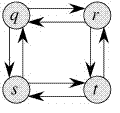
\includegraphics[width=0.2\linewidth]{images/LongestPath.png}

\subsection{Worked example: possible ways to sum coins}
Imagine there was a currency with coins of value 1, 5 and 7. The task is to list all possible combinations of these basic coins to obtain a total value of $n$.


Here is an idea how this could be implemented: 
Lets call our function \inlinecode{combs(n)}.
Add 1 to each list in the results of \inlinecode{combs(n-1)},
add 5 to each list in the results of \inlinecode{combs(n-5)}, 
and add 7 to each list in the results of \inlinecode{combs(n-7)}.


\begin{lstlisting}[language=python]

def combs(n):
	if n < 1:
		return []
	if n == 1:
		return [[1]]
	if n == 5:
		return [[1,1,1,1,1],[5]]
	if n == 7:
		return [[1,1,1,1,1,1,1],[5,1,1],[1,5,1],[1,1,5],[7]]

	list1 = combs(n-1)
	list5 = combs(n-5)
	list7 = combs(n-7)

	fullList = []
	for c in list1:
		fullList.append(c + [1])
	for c in list5:
		fullList.append(c + [5])
	for c in list7: 
		fullList.append(c + [7])

	return fullList

\end{lstlisting}

Now just add some caching, and you have an efficient algorithm as well. 

Verify that this idea shows overlapping subproblems
and that it shows optimal substructure

Proof that algorithm delivers correct results


counterexample: minimal number of coins


\subsection{A strategy for finding the recursion}

Dynamic programming tries to solve problems by breaking them apart into subproblems. But how do we find those subproblems?

The solution $S$ we are looking for should be obtained by some function $sol$.
$$ S = sol(para) $$

Try to find a way to split $S$ into a large part $S'$ and a small part $s$ \marginnote{In more advanced problems we might instead want to partition $S$ into several new sets $S'$ and $S''$}.
$$ S = S' + \{ s \} $$

The large part itself must be the result of $sol$ for some other set of parameters $para'$.
$$ S' = sol(para') $$





\subsection{Markow chains}

\subsection{Markov decision process with known state-transition-function}

MDPs are an extension of Markov chains, they add actions (allowing choice) and rewards (giving motivation). Conversely, if only one action exists for each state (e.g. "wait") and all rewards are the same (e.g. "zero"), a Markov decision process reduces to a Markov chain. 

An MDP is a tuple $(S, A, P_a, R_a)$, where 
\begin{itemize}
	\item $S$: finite set of states
	\item $A$: finite set of actions
	\item $P_a(s, s') = P(s_{t+1} = s' | s_t = s, a_t = a)$
	\item $R_a(s, s')$ is the immediate reward received after transitioning from $s$ to $s'$ through action $a$.
\end{itemize}

The goal is to find a policy $\pi(s) = a$ that maximizes the cumulative reward $\sum_{t=0}^\infty \gamma_t R_{a_t}(s_t, s_{t+1})$, where $\gamma_t$ is the discount-factor. The discount factor is used so that the decision maker favours taking actions early and doesn't postpone them indefinitely. 

Because of the Markov property, the optimal policy for this particular problem can indeed be written as a function of $s$ only, as assumed above.



\subsection{Reinforcement learning: MDP without explicitly known state-transition-function}


\section{Calculus}

\subsection{Hyperreals}

For the biggest part, we're going to deal with Nelson-style nonstandard-analysis. 

List of external properties:
\begin{itemize}
    \item std, nstd
    \item limt, nlimt
    \item inftsm, inft
    \item nearly cont
\end{itemize}

A statement using any external properties will be denoted as $\ext{A}$, one that \emph{might} use external properties as $\pext{A}$.

We will use the following axioms:
\begin{enumerate}
    \item $0:std$
    \item $\forall n \in \naturals: n:std \then (n+1):std $
    \item $\thereis n \in \naturals: n:nstd $
    \item External induction: Induction  over \std{n} about \pext{A}: \\ 
    $ [ \pext{A}(0) \land \forall \std{n} \in \naturals: \pext{A}(n) \then \pext{A}(n+1) ] \then \forall \std{n} \in \naturals: \pext{A}(n)$
    \item Internal induction: Induction over \pnstd{n} about A: \\
    $ [A(0) \land \forall \pnstd{n} \in \naturals: A(n) \then A(n+1)] \then \forall n \in \naturals: A(n) $
\end{enumerate}

The rationale over the two induction-axioms is simple. Ordinary induction is about $A$ over \std{n}. 
External induction is about \pext{A} over \std{n}. This makes sure that statements about external stuff only apply to finite $n$, not to infinite ones. 
Internal induction is about $A$ over \pnstd{n}. This makes sure that when we talk about potentially infinite $n$'s, we only apply internal statements.

In other words: these two inductions ensure that we \textbf{never apply external statements to external numbers}. 

Doing so would lead to logical incosistencies. That's why there is no "fully external" induction.

However, note that axiom 2 is actually a case of "fully external" induction.


\begin{theorem}
    $ \forall n \in \naturals: n:nst \then (n+1):nst $ \label{addingNonstds}
\end{theorem}
\begin{proof}
    \subprf{Suppose $n:nst$.}{$(n+1):nst$}{
        \subprf{By contradiction. Suppose $(n+1):std$.}{this leads to a contradiction.}{
            $(n+1):std \then n:std$.  \\
            This contradicts the premise that $n:nst$.
        }
    }
\end{proof}

If you don't believe the argument in the previous proof, consider this: 
\begin{proof}
    \subprf{
    Suppose all of the following: \\
    $ [\forall n: Q(n) \then Q(n+1)] \then \forall n: Q(n) $ \\
    $ [\forall n: Q(n) \then Q(n+1)] $ \\
    This leads to $ \forall n: Q(n) $. \\ 
    }{$ \forall n: Q(n+1) \then Q(n) $}{
        \subprf{Let $n = n_0$ and suppose $Q(n_0+1)$.}{$Q(n_0)$}{
            Since $ \forall n: Q(n) $ holds, it must be true that $Q(n_0)$.
        }
    }
\end{proof}


We can use theorem \ref{addingNonstds} to prove the following: 

\begin{theorem}
    $\forall n, m \in \naturals: n:std \land m:nstd \then (n+m):nst$
\end{theorem}
\begin{proof}
    \subprf{Let $m=m_0:nst$.}{$\forall n \in \naturals: n:std  \then (n+m_0):nst$}{
        By induction on $n$. 
        \\
        \subprf{Base case. Let $n=0$.}{$(0+m_0):nst$}{
            $0+m_0=m_0$ \\
            $m_0:nst$
        }
        \\
        \subprf{Induction step.}{$[(n+m_0):nst] \then [(n+1+m_0):nst]$}{
            Just apply theorem \ref{addingNonstds} to $n=(n+m_0)$.
        }
    }
\end{proof}

It is notable that you can never reach a standard number when adding nonstandard numbers.
\begin{theorem}
    $ \forall n,m \in \naturals: n,m:nst \then (n+m):nst $
\end{theorem}
\begin{proof}
    We proceed by proving the equivalent $ (n+m):std \then (n:std \lor m:std) $ 
    \subprf{Suppose $(n+m):std$}{$(n:std \lor m:std)$}{
        \subprf{Without loss of generality, suppose $n:nst$}{$m:std$}{
            \subprf{By contradiction. Suppose $m:nst$}{this leads to a contradiction}{
                We have already assumed that  $(n+m):std$. \\
                Now, however, we also assume that $n,m:nst$. \\
                Using theorem \ref{addingNonstds} however, we see that when $n,m:nst$, then it must be that $(n+m):nst$.
            }
        }
    }
\end{proof}


\subsection{Limits}

\subsection{Sequences and series}

\subsubsection{Tailor}
\subsubsection{Fourier}
\subsubsection{Laplace}

\subsection{Euler's formula}
Proof: Consider the function $f(t)=e^{-it}(cost+isint)$ for $t \in \reals$. By the quotient rule
$$ f'(t) = e^{-it} (i\ cos(t) - \sin(t)) -ie^{-it} (\cos(t) + i \sin(t)) = 0 $$
identically for all $t \in \reals$. Hence, $f$ is constant everywhere. Since $f(0)=1$, it follows that $f(t)=1$ identically. Therefore, $e^{it}=cost+isint$ for all $t \in \reals$, as claimed.


\subsection{Integration}

The infinitessimal view of calculus makes it quite easy to prove theorems. Consider this illustration of how definite integrals work.

\begin{equation}
    \begin{aligned}
        \int_a^b \frac{dF}{dx}(x) dx &= \int_a^b \frac{F(x + dx) - F(x)}{dx} dx \\
        \int_a^b F(x + dx) - \int_a^b F(x) &= F(b + dx) - F(a)
    \end{aligned}
\end{equation}


\subsubsection{Integration strategies}

\paragraph{u-substitution}

\paragraph{Integration by parts} is the last trick up our sleave when all other strategies haven't helped. Consider the integral 

$$ \int x e^x \diff{x} $$

We can rewrite this integral as 

$$ \int u \diff{v} $$

where $u = x$ and $\diff{v} = e^x \diff{x}$. In general, you always want to pick $u$ in such a way that $u$ gets simpler after being differentiated.
$x$ does get a lot simpler after differentiation, whereas $e^x$ doesn't, so the choice is clear. 

We then use the following: 

$$ \int u \diff{v} = uv - \int v \diff{u} $$\footnote{The proof goes like this: Starting with the product rule of differentiation: $(ab)' = a'b + ba'$ we get $(ab)' - a'b = ba'$ and  $ab - \int a'b \diff{x} = \int ba' \diff{x} $}

Since we chose $u = x$ we have $\diff{u} = \diff{x}$, and from $\diff{v} = e^x \diff{x}$ we get $v = e^x$. This yields us: 

$$ xe^x - \int e^x \diff{x} $$
$$ e^x ( x - 1) $$

as the solution. 

\subsection{Vector calculus}

Integration over a vector, integration along a vector, integration along a surface. 

You can find a nice introduction (mostly in the second part of) this pdf: \inlinecode{http://www.maths.gla.ac.uk/~cc/2A/2A_notes/2A_chap4.pdf} and here \inlinecode{http://geocalc.clas.asu.edu/pdf-preAdobe8/SIMP_CAL.pdf}


\subsubsection{Constraint optimization using Lagrange multipliers}

We want to maximize $f(x, y)$ subject to the constraint $g(x, y) = 0$.
At the optimal point $x_0, y_0$ it must hold that:
\begin{equation}
  \nabla f = \lambda \nabla g
\end{equation}
for some scalar $\lambda$ (the so-called Lagrange-multiplier).

Example:
$$ f(x, y) = x^2 y $$
$$ g(x, y) = x^2 + y^2 = 1 $$

Now using $\nabla f = \lambda \nabla g$ we get the system of equations:
\begin{equation}
    \begin{aligned}
        2xy &= 2x\lambda \\
        x^2 &= 2y\lambda \\
        x^2 + y^2 &= 1
    \end{aligned}
\end{equation}

Which yields $x = \sqrt{2/3}$, $y = \sqrt{1/3}$ and $\lambda = \sqrt{1/3}$.

%\section{Differential equations}


\section{Number theory}

\subsection{Divisability}

\begin{definition}
    Divisability: $a|b \iff \thereis k: ak = b$
\end{definition}

\begin{theorem}
    $ a|b \land b|c \then a|c  $
\end{theorem}

\begin{proof}
    \subprf{}{$a|b \land b|c \then a|c$}{
        \subprf{Suppose $ \thereis x_0 : ax_0 = b \land \thereis x_1 : bx_1 = c $}{$\thereis x_2 : ax_2 = c$}{
            Try $ x_2 = x_0 x_1 $ \\
            Then $ a x_2 = a x_0 x_1 = b x_1 = c $
        }
    }
\end{proof}

\begin{theorem}
    If a divides both b and c, then a divides any linear combination of b and c as well.  $ a|b \land a|c \then \forall v, w: a| (vb + wc)  $
\end{theorem}

\begin{proof}
    \subprf{}{$ a|b \land a|c \then \forall v, w: a| (vb + wc)  $}{
        \subprf{Suppose $ a|b \land a|c$}{$\forall v, w: a | (vb + wc)  $}{
            \subprf{Let $v_0, w_0$}{$ \thereis x : ax = (v_0 b + w_0 c) $}{
                Try $ x = v_0 x_0 + w_0 x_1 $
            }
        }
    }
\end{proof}

\begin{definition}
    Modulus: $ a\%d = r \iff d|(a-r) \land 0 \leq r \leq d $
\end{definition}


\subsection{Hashing}

\subsection{Encryption}

\subsubsection{Symmetric encryption}

\subsubsection{Asymmetric encryption}

The basic idea of the Diffie-Hellman algorithm is as follows: instead of a secret key used for encryption and decryption, use a two-part-key. We can then find an algorithm where only the public part of the key is ever visible to Eve. 

Here is an analogy:
\begin{itemize}
	\item You have a lock (pubK) and a key (prvK). Send your lock publically to Bob, while you keep your key hidden in your vest. 
	\item Bob writes his message to you and locks it with your lock in a box. Neither he nor Eve can now open the box again. Bob sends the box to you.
	\item You open the box with your key and read the message
\end{itemize}

\includegraphics[]{images/diffie_hellman}

This general concept is known as Diffie-Hellman asymmetric encryption. To implement it, one needs 
\begin{itemize}
	\item A function to generate a key-pair
	\item A function for encryption using the message and another persons public key
	\item A function for decryption using a cypher and your own private key
\end{itemize}
The first successful implementation of this principle is known as the WPA algorithm. 

\paragraph{In practice} WPA takes too long to be used very often, whereas symmetric encryption is much faster. For this reason, one usually follows a two step process:
\begin{itemize}
	\item create a new symK
	\item exchange that symK via WPA
	\item use the symK to do symmetric encryption
\end{itemize}


\section{Artificial intelligence}

\subsection{Categorisation}

\subsubsection{Neural networks}

\paragraph{Backpropagation networks}

There are two ways in which we can derive the backpropagation-algorithm. One is purely analytical, the other bayesian. We'll demonstrate both. 

\paragraph{The analytical way of deriving the backpropagaion algorithm} consist of just a few steps. 
A few definitions: 

\begin{itemize}
	\item A layers outputvector $\vec{y}^l$ is obtained by the activation function $\vec{y}^l = f(\vec{x}^l) $
	\item The layers inputvector is obtained as a weighted sum of previous outputs: $\vec{x}^l = \mtrx{W}^l \vec{y}^{l-1} $. We cn express a single $x_t^l = \sum_f W_{t,f}^l y_f^{l-1}$
	\item We strive to minimize the error-function. Assuming only one single training item we get $e = \frac{1}{2} \sum_t (\vec{y}^*_t - \vec{y}^L_t)^2 $
\end{itemize}

Let's first consider only the top layer. 

$$  \partDiff{e}{x_{t_0}^L} = \frac{1}{2} \sum_t \partDiff{}{x_{t_0}^L} (\vec{y}^*_t - \vec{y}^L_t)^2 $$
$$ = (y_{t_0}^* - y_{t_0}^L) f'(x_{t_0}) $$

Or, in vector form: 

$$ \partDiff{e}{\vec{x}^L} = (\vec{y}^* - \vec{y}^L)^T \pointwise f'(\vec{x}^L)  $$


That part was easy. But how do we obtain the same differential for \emph{any} layer $l$?

$$ \partDiff{e}{x_{f_0}^l} = \sum_t \partDiff{e}{x_t^{l+1}} \partDiff{x_t^{l+1}}{x_{f_0}^l}  $$
$$                         = \sum_t \partDiff{e}{x_t^{l+1}} \partDiff{}{x_{f_0}^l} ( \sum_f W_{t,f}^{l+1} y_f^l ) $$
$$                         = \sum_t \partDiff{e}{x_t^{l+1}} W_{t,f_0}^{l+1} f'(x_{f_0}^l)  $$

Or, in vector form: 

$$ \partDiff{e}{\vec{x}^l} = ( \mtrx{W}^{l+1}^T \partDiff{e}{\vec{x}^{l+1}} ) \pointwise f'(\vec{x}^l)  $$

The smart part here was to not derive $ \partDiff{e}{\vec{x}^l} $ by going through $\vec{y}^L$, $\vec{x}^L$, $\mtrx{W}^L$, $\vec{y}^{L-1}$, $\vec{x}^{L-1}$, $\mtrx{W}^{L-1}$, ..., but by instead creating a recurrence relation by differentiating by $\vec{x}^{l+1}$.

Finally, we can obtain the gradient at our weights as: 

$$ \partDiff{e}{W_{t_0, f_0}^l} = \partDiff{e}{x_{t_0}^l} \partDiff{x_{t_0}^l}{W_{t_0, f_0}^l}   $$
$$                              = \partDiff{e}{x_{t_0}^l} \partDiff{}{W_{t_0, f_0}^l} ( \sum_f W_{t_0, f}^l y_f^{l-1} ) $$
$$                              = \partDiff{e}{x_{t_0}^l} y_{f_0}^{l-1} $$

Or, in vector form: 

$$ \partDiff{e}{\mtrx{W}^l} = \partDiff{e}{\vec{x}^l} \outerp \vec{y}^{l-1} $$ 

So we should change the weigths by: 

$$ \Delta \mtrx{W}^l = - \alpha \partDiff{e}{\mtrx{W}^l} $$
$$ = \partDiff{e}{\vec{x}^l} \vec{y}^{l-1} $$


It makes sense to reitterate the whole process in matrix-form. 

First, we  get $\delta^L$:
$$ \partDiff{e}{\vec{y}^L} = (\vec{y}^* - \vec{y}^L)^T := \delta^L $$ 

Then we go through the highest layer:
$$ \partDiff{e}{\vec{x}^L} = \delta^L \pointwise f'(\vec{x}^L)  $$
$$ \partDiff{e}{\mtrx{W}^L} = \partDiff{e}{\vec{x}^L}^T \vec{y}^{L-1}^T $$
$$ \delta^{L-1} = \partDiff{e}{\vec{x}^L} \mtrx{W}^L $$

Then we pass $\delta^{L-1}$ to the next layer. 
$$ \partDiff{e}{\vec{x}^l} = \delta^l \pointwise f'(\vec{x}^l)  $$
$$ \partDiff{e}{\mtrx{W}^l} = \partDiff{e}{\vec{x}^l}^T \vec{y}^{l-1}^T $$
$$ \delta^{l-1} = \partDiff{e}{\vec{x}^l} \mtrx{W}^l $$




\paragraph{Gaussian processes}

The bayesian derivation of the backpropagation algorithm gives rise to the interesting idea that backprop-networks may be generalized into ...

\paragraph{Convolutional networks}

These are the networks most commonly found employed as a deep-learning architecture. Really, they are just a simplified version of our backpropagation-networks (they are even trained using an only slightly altered algorithm). Instead of connecting every node from layer $l$ to every node of layer $l+1$, they impose some restrictions on the connection-matrix:
\begin{itemize}
	\item Nodes are connected in a pyramid scheme. A node on layer $l+1$ is connected to 9 nodes directly beneath it. Instead of a $n_l \times n_{l+1}$ connection matrix, we thus have several $9 \times 1$ matrices.
	\item The connection-strengths of these  $9 \times 1$ matrices are all the same - so really there is only just one  $9 \times 1$ matrix. 
\end{itemize}
These restrictions are inspired by the physiology of the visual cortex. They have the nice effect that a network is trained much faster, since they massively reuce the ammount of weights that need to be learned. 

\subsection{Computer vision}

\paragraph{Feature detection and pose estimation}

Say you want to locate the position of the nose in a portrait. 


\chapter{Algorithms and data-structures}
\section{General algorithm theory}

\subsection{Invariant principle}

The invariant principle is not much more than using induction to prove that some statement holds over all iterations $n$ from $0$ to $n_0$.


\subsection{Well ordering}

The well ordering principle is a fundamental theorem in discrete mathematics. 

$$ \forall S \subset \naturals^+: S \neq \emptyset : \thereis x_0 \in S: \forall x \in S: x_0 \leq x $$

We usually use it in existance proofs, by contradiction. However, there is a nice little template for proofs using the well ordering principle.

To prove that $P(n)$ holds true for $\forall n \in \naturals$:

\begin{itemize}
    \item Define the set $C$ of counterexamples to $P$ being true. That is: 
    $$ C = \{ n \in \naturals | \lnot P(n) \}$$
    
    \item For a proof by contradiction, assume $C$ is nonempty.
    
    \item By the well ordering principle, there will be a smallest element $n_0 \in C$
    
    \item Reach a contradiction (often by showing how to use $n_0$ to find another member of $n_1 \in C$ that is even smaller than $n_0$)
\end{itemize}


\subsection{Programm verification according to Floyd}

If the following properties are given, then an algorithm is be correct. 

\begin{itemize}
    \item Partial correctness: if an answer is returned, it will be correct.
    \item termination: The algorithm eventually reaches a halt - meaning that an answer is always returned eventually. 
\end{itemize}

There is a simple method of proving an algorithm correct (by Floyd ):
\begin{itemize}
    \item Proving 'partial correctness' with invariant principle: there is some loop invariant that basically says: 'At this iteration the state is a little better than before'. For example, in a sorting problem, at the i'th iteration the subarray \inlinecode{data[0:i]} might already be sorted. 
    \item Proving 'termination' with well ordering principle
\end{itemize}

Note that there might be correct algorithms that don't have these properties. For example, some algorithms might eventually reach a desired state without ever having an ever-imporving loop invariant. Also, there are other ways to prove an algorithm correct than the Floyd-method. However, in many real-world examples, this is the easiest approach to formaly proving an algorithm correct. 

\subsubsection{ Proving 'partial correctness' with invariant principle }



\subsubsection{ Proving 'termination' with well ordering principle }


\subsection{Notation}

An algorithm that takes $f(n)$ cycles is said to take \BigTheta{g(n)} time, iff: 

$$ f \in \BigTheta{g(n)} $$ 
where 
$$ \BigTheta{g(n)} = \{ f(n) | \thereis c_1, c_2, n_0 : \forall n \geq n_0:  0 \leq c_1 g(n) \leq f(n) \leq c_2 g(n) \} $$

Simmilarly, the set \BigOh{g(n)} is defined as: 
$$ \BigOh{g(n)} = \{ f(n) | \thereis c_2, n_0 : \forall n \geq n_0:  0 \leq  f(n) \leq c_2 g(n) \} $$

That is, \BigOh{} only has an upper bound, but no lower bound.

\subsection{Order of basic operations}

In the integer ram model of computation, addition, multiplication, remainder and bitwise operations all take O(1).


\subsection{Remembering the state in loops}
Sometimes, operations have to be repeatedly executed in a loop. These operations may take \BigOh{g} time by themselves, but only \BigOh{1} time if the result of the previous execution is already known. 

In such a case it makes sense to keep track of the previous result. StateMachines are a natural vehicle to store such information. 

Lets assume for now that modulo was not constant time. Then we could do the infamous FizzBuzz problem like this in linear time: 

\begin{lstlisting}[language=python]
class SM:
    def __init__(self, nr):
        self.nr = nr
        self.nToGo = nr

    def feed(self):
        self.nToGo -= 1
        if self.nToGo < 0:
            self.nToGo = self.nr - 1

    def isMult(self):
        return self.nToGo == 0



threeM = SM(3)
fiveM = SM(5)
for i in range(1, 16):
    threeM.feed()
    fiveM.feed()
    if threeM.isMult() and fiveM.isMult():
        print("{} --> FizzBuzz".format(i))
    elif threeM.isMult():
        print("{} --> Fizz".format(i))
    elif fiveM.isMult():
        print("{} --> Buzz".format(i))
    else:
        print(i)
\end{lstlisting}

\subsection{Dynamic programming}
A natural extension to the idea above here is dynamic programming. There we also make use of the fact that some instructions can be simplified if we remember the result of the previous instruction.


\subsection{Solving recurrences}
Sometimes we dont have to do a recursive sollution at all. Many recursive problems can be reshaped into a explicit form (the so called closed form). Think of the Fibonacci-sequence: 

$$ fib(n) = fib(n-1) + fib(n-2) = \frac{(1 + \sqrt{5})^n - (1 - \sqrt{5})^n }{2^n \sqrt{5}} $$

This section will examplify some methods for finding the closed form expression.

\subsubsection{Solving linear recurrences}

A homogeneous linear recurrence is one of the following form: 

$$ f(n) = a_1 f(n-1) + a_2 f(n-2) + ... + a_d f(n-d)$$

We can solve it as follows: 

\begin{enumerate}
    \item Assume $f(n) = x^n$. We now try to find an expression for $x$.
    \item Divide both sides in the hlr by $x^{n-d}$, leaving a (hyper-)quadratic equation. 
    \item Every root of the quadratic equation is a \textbf{homogeneous sollution}. Also, if a root $r$ occures $v$ times, $r^n, nr^{n-1}, n^2r^n ..., n^{v-1}r^n$ are also sollutions.
    \item Also, every linear combination of the above is also a sollution. So, a sollution might in general have a form like $a r_1^n + b r_2^n + ...$.
    \item Finally, choose $a, b, ...$ such that they fulfill the boundary conditions (in Fibonacci those would be $f(0) = f(1) = 1$). This is the \textbf{concrete sollution}.
\end{enumerate}

We can extend the above schema to also solve (nonhomogeneous) linear recurrences: 
$$ f(n) = a_1 f(n-1) + a_2 f(n-2) + ... + a_d f(n-d) + g(n)$$

\begin{enumerate}
    \item Ignore $g(n)$, find the homogeneous sollution from step 4 above.
    \item Find a \textbf{particular sollution} to the equation including $g(n)$.
    \item homogeneous solltution + particular sollution = \textbf{general sollution}
    \item Now for the general sollution, again plug in the boundary conditions as in step 5 above.
\end{enumerate}


\section{Important algorithms}

\subsection{Merge-sort}

The function merge takes two already sorted lists and merges them into one sorted list.

\begin{lstlisting}[language=python]
def merge(a, b):
    c = []
    ia = ib = ic = 0
    while len(c) < len(a) + len(b):
        if a[ia] <= b[ib]:
            c[ic] = a[ia]
            ia++
        else:
            c[ic] = b[ib]
            ib++
        ic++
    return c
\end{lstlisting}

\invariant{statement}{sometext}{sometext}{sometext}


\subsection{Matrix inverse}
Gauss Jordan

\subsection{Polynomals}

In this section, we will deal with the polynomal $P_A(x) = 1x^3 + 2x^2 + 3x + 4$. Working with polynomals turns out to be quite important in everyday practice - especially when you're working with generating functions.

\subsubsection{Coefficient-representation of polynomals}
The most common representation of this polynomal is its coefficient representation $[4, 3, 2, 1]$. This representation is very convenient for fast evaluation at any $x$ using Horner's method: 

\begin{lstlisting}[language=c]
#include "stdio.h"
#include "stdlib.h"
#include "math.h"

/**
 * Coefficient representation of polynomals
 */

typedef struct PolynomalC {
  int length;
  int* coefficients;
} PolynomalC;

PolynomalC* polyc_create(int l, int* coeffs) {
  PolynomalC* p = malloc(sizeof(PolynomalC));
  p->length = l;
  p->coefficients = malloc(l*sizeof(int));
  for(int i = 0; i<l; i++){
    p->coefficients[i] = coeffs[i];
  }
  return p;
}

void polyc_delete(PolynomalC* p) {
  free(p->coefficients);
  free(p);
}

int polyc_evalAt(PolynomalC* p, int x) {
  int sum = 0;
  for(int i = p->length; i > 0; i--){
    sum = sum * x + p->coefficients[i-1];
  }
  return sum;
}

PolynomalC* polyc_add(PolynomalC* p1, PolynomalC* p2) {
  int l1 = p1->length;
  int l2 = p2->length;
  int l = max(l1, l2);
  int coeffs[l];
  for(int i = 0; i < l; i++){
    int v = 0;
    if(i < l1) v += p1->coefficients[i];
    if(i < l2) v += p2->coefficients[i];
    coeffs[i] = v;
  }
  PolynomalC* p3 = polyc_create(l, coeffs);
  return p3;
}

int main(void) {
  
  int coeffs1[4] = {4, 3, 2, 1};
  PolynomalC* p1 = polyc_create(4, coeffs1);
  
  int coeffs2[3] = {1, 2, 3};
  PolynomalC* p2 = polyc_create(3, coeffs2);
  
  PolynomalC* p3 = polyc_add(p1, p2);
  
  int r = polyc_evalAt(p3, 2);
  printf("Result: %d\n", r);
  
  polyc_delete(p1);
  polyc_delete(p2);
  polyc_delete(p3);
  
  return 0;
}
\end{lstlisting}

\subsubsection{Point-value-representation of polynomals}
Another way of representing this polynomal is the point-value representation $[(0,4), (1, 10), (2, 26), (3,58)]$. This representation is very convenient for fast evaluation of polynomal multiplication (assuming both polys are evaluated at exactly the same points): 

\begin{lstlisting}[language=c]
#include "stdio.h"
#include "stdlib.h"
#include "math.h"

/**
 * Point/Value representation of polynomals
 */

typedef struct PolynomalV {
  int length;
  int* points;
  int* values;
} PolynomalV;

PolynomalV* polyv_create(int l, int* pts, int* vls) {
  PolynomalV* p = malloc(sizeof(PolynomalV));
  p->length = l;
  p->points = malloc(sizeof(int)*l);
  p->values = malloc(sizeof(int)*l);
  for(int i = 0; i < l; i++) {
    p->points[i] = pts[i];
    p->values[i] = vls[i];
  }
  return p;
}

void polyv_delete(PolynomalV* p) {
  free(p->points);
  free(p->values);
  free(p);
}

PolynomalV* polyv_mult(PolynomalV* p1, PolynomalV* p2) {
  int l = p1->length;
  int vals[l];
  for(int i = 0; i < l; i++) {
    vals[i] = p1->values[i] * p2->values[i];
  }
  PolynomalV* p = polyv_create(l, p1->points, vals);
  return p;
}

int main(void) {
  
  int points[4] = {0, 1, 2, 3};
  
  int vals1[4] = {4, 10, 26, 58};  // [4, 3, 2, 1]
  PolynomalV* p1 = polyv_create(4, points, vals1);
  
  int vals2[4] = {1, 10, 49, 142}; // [1, 2, 3, 4]
  PolynomalV* p2 = polyv_create(3, points, vals2);
  
  PolynomalV* p3 = polyv_mult(p1, p2);
  
  polyv_delete(p1);
  polyv_delete(p2);
  polyv_delete(p3);
  
  return 0;
}
\end{lstlisting}

\subsubsection{Naive transformation from coefficient to point-value and vice-versa}
\begin{lstlisting}[language=c]

// O(n^2)
 PolynomalV* poly_coeffToPv(PolynomalC* pc, int* points){
   int l = pc->length;
   int vals[l];
   for(int i = 0; i < l; i++) { // n operations
     vals[i] = polyc_evalAt(pc, points[i]); // O(n)
   }
   PolynomalV* pv = polyv_create(l, points, vals);
   return pv;
 }

// O(n^3)
PolynomalC* poly_PvToCoeff(PolynomalV* p){
  int l = p->length;
  int points[l] = p->points;
  int values[l] = p->values;
  int** data = [[1, x1, x1^2, ...]
                [1, x2, x2^2, ...]
                [1, x3, x3^2, ...]];
  Matrix* m = mtrx_create(l, l, data);
  Matrix* mi = mtrx_inverse(m);   // Gauss Jordan: O(n^3)
  int coeffs[l] = mtrx_mult(mi, values);
  PolynomalC* pc = polyc_create(l, coeffs);
  return pc;
}


int main(void) {
  
  int coeffs[4] = {4, 3, 2, 1};
  PolynomalC* pc = polyc_create(4, coeffs);
  int points[4] = {0, 1, 2, 3};
  PolynomalV* pv = poly_coeffToPv(pc, points);
  PolynomalC* px = poly_PvToCoeff(pv);
  
  polyc_delete(pc);
  polyv_delete(pv);
  polyc_delete(px);
  
  return 0;
}
\end{lstlisting}

\subsubsection{Fast transformation}
Up to now we have used the points $0, 1, 2, 3$ for our evaluation. However, there is no reason why we should have chosen these specific points - any other points of evaluation are just as good. It turns out that if we use the 4 roots of 1 as points of evaluation, we can cut down on computation costs.

In general, the $k$th root of 1 is $e^{2 \pi i \frac{k}{n} }$. So let's do the evaluation at $(1^{1/4})_1, (1^{1/4})_2, (1^{1/4})_3, (1^{1/4})_4 = 1, i, -1, -i$.



\subsection{Stream algorithms}
Stream algorithms handle the case where a function is not applied once for a single input, but continuously on a neverending stream of inputs. This creates some constraints: 
\begin{itemize}
  \item The algorithm must not take longer than the feed-rate of the stream
  \item The algorithm must use only a constant ammount of storage (because otherwise at some point the disc will be full)
\end{itemize}
\href{https://www.americanscientist.org/article/the-britney-spears-problem}{Here} is a good introduction to the toppic. 
Sidenote: a popular software to provide a stream to (multiple) subscriber(s) would be \href{https://kafka.apache.org/}{Apache kafka}.
\section{Data-structures}

\subsection{Stack}

Stacks perform push and pop in O(1).
However, they do search in O(n).

\begin{lstlisting}[language=c]
#include <stdio.h>
#include <stdlib.h>
#include <string.h>



typedef struct El {
	char* key;
	float val;
} El;


El* el_create(char* key, float val){
	char* keyk = strdup(key);
	El* el = malloc(sizeof(El));
	el->key = keyk;
	el->val = val;
	return el;
}


void el_destroy(El* el){
	free(el->key);
	free(el);
}


typedef struct Stack {
	El** data;
	int size;
	int top;
} Stack;


Stack* stack_create(int size){
	Stack* stack = malloc(sizeof(Stack));
	stack->data = malloc(sizeof(El*) * size);
	stack->size = size;
	stack->top = -1;
	return stack;
}

void stack_push_el(El* el, Stack* stack){
	stack->top += 1;
	stack->data[stack->top] = el;
}

void stack_push(char* key, float val, Stack* stack){
	El* el = el_create(key, val);
	stack_push_el(el, stack);
}

El* stack_pop(Stack* stack){
	stack->top -= 1;
	return stack->data[stack->top + 1];
}

El* stack_peak(Stack* stack){
	return stack->data[stack->top];
}

void stack_print(Stack* stack){
	int i;
	for(i = 0; i <= stack->top; i++){
		printf("%s -> %d", stack->data[i]->key, stack->data[i]->val);
	}
}

void stack_destroy(Stack* stack){
	while(stack->top >= 0){
		El* el = stack_pop(stack);
		el_destroy(el);
	}
	free(stack->data);
	free(stack);
}


int main(){

	Stack* s = stack_create(10);
	stack_push("eins", 1.1, s);
	stack_push("zwei", 1.2, s);
	stack_push("drei", 3.1, s);

	stack_print(s);

	stack_destroy(s);

	return 0;

}

\end{lstlisting}

\subsection{Linked lists}

Linked lists have the advantage that they have no prefixed size. Addition and insertion at any point is O(1). On the other hand, searching takes O(n) in the worst case. 


\subsection{Binary trees}

Trees make sense when the keys have to be ordered in some sense. 

\begin{lstlisting}[language=c]
#include <stdio.h>
#include <stdlib.h>
#include <string.h>



typedef struct El {
	int key;
	float val;
} El;


El* el_create(int key, float val){
	El* el = malloc(sizeof(El));
	el->key = key;
	el->val = val;
	return el;
}


void el_destroy(El* el){
	free(el);
}

typedef struct Node {
	struct El* data;
	struct Node* parent;
	struct Node* left;
	struct Node* right;
} Node;


Node* node_create(Node* parent, El* element){
	Node* leaf = malloc(sizeof(Node));
	leaf->parent = parent;
	leaf->data = element;
	return leaf;
}

void node_destroy(Node* node){
	if(node->left != NULL){ node_destroy(node->left); }
	if(node->right != NULL){ node_destroy(node->right); }
	el_destroy(node->data);
	free(node);
}

void node_elementInsert(Node* node, El* el){
	if(el->key < node->data->key){
		if(node->left){
			node_elementInsert(node->left, el);
		}else{
			node->left = node_create(node, el);
		}
	}else{
		if(node->right){
			node_elementInsert(node->right, el);
		}else{
			node->right = node_create(node, el);
		}
	}
}

void node_dfsPrint(Node* node){
	printf("%d -> %d \n", node->data->key, node->data->val);
	if(node->left){
		node_dfsPrint(node->left);
	}
	if(node->right){
		node_dfsPrint(node->right);
	}

}

typedef struct Tree {
	Node* root;
} Tree;


Tree* tree_create(El* el){
	Tree* tree = malloc(sizeof(Tree));
	Node* root = node_create(NULL, el);
	tree->root = root;
	return tree;
}

void tree_destroy(Tree* tree){
	node_destroy(tree->root);
	free(tree);
}

void tree_elementInsert(Tree* tree, El* el){
	node_elementInsert(tree->root, el);
}

void tree_dfsPrint(Tree* tree){
	node_dfsPrint(tree->root);
}


int main(){

	El* baseEl = el_create(20, 14);
	El* el1 = el_create(1, 4);
	El* el2 = el_create(25, 9);
	El* el3 = el_create(2, 2);

	Tree* tree = tree_create(baseEl);

	tree_elementInsert(tree, el1);
	tree_elementInsert(tree, el2);
	tree_elementInsert(tree, el3);

	tree_dfsPrint(tree);

	tree_destroy(tree);
	return 0;

}

\end{lstlisting}

\subsection{Hash-tables}

Hash tables are basically a array with a hash-function. The hash function is there to associate string-keys to the integer-array-indices. The array needs as many elements as the hash-function can create integer-keys. 

Through the hash-function the hash-table has insertion- and lookup-times of expected O(1). However, when the array gets many elements. it might happen that the hash-function gives the same integer-key to several string-keys. To acommodate such a case, the array-elements are implemented as linked lists. This makes the worst-case loopup-time O(n/k).


Why does one not simply use a perfect hash? Make a hash-function that generates a unique key for any string it's given. This would be known as a lookup-table. That works perfectly fine when we expect almost all possible string-keys to be really used. If however we  expect only a few of the possible strings to be used, the array would contain a lot of unused space.

\chapter{General computer theory}
\section{Hardware}

\subsection{Memory}


Data is moved from ram to the processor by the memory controller. 


Each cell in memory holds 8 bits. 

\subsubsection{How data is stored}

\begin{itemize}
    \item  \inlinecode{tiny int}: use just one bite - making 256 possible values. 
   \item  \inlinecode{int}: uses 4 bites (32 bits)
   \item  \inlinecode{long int}: uses 8 bites (64 bits)
   \item  \inlinecode{signed int}: reverse the leftmost bit
   \item  \inlinecode{fractions}: store two numbers: the numerator and the denominator. 
   \item  \inlinecode{float}: also store two numbers: the number without the point and the position of the point
\end{itemize}


Fun fact: java tends to silently cause integer overflows. When it has to compute an addition of two big ints, say 255 + 1 (1111 1111 + 0000 0001), it does the right computation (1 0000 0000) but throws away the leftmost binary because that won't fit into memory, causing the result to be stored as 0000 0000. 

\begin{lstlisting}[language=java]
System.out.println(Integer.MAX_VALUE);   
Integer a = 2147483647;
Integer b = 1;
Integer c = a + b;
System.out.println(c);
\end{lstlisting}


Words and Pages:



\subsection{Processors}

Processors have a cache where they store copies of stuff they recently read form ram. This cache is even faster than reading from ram itself. Because programs tend to put their stuff in sequential order in the ram, the memory controller not only feeds the processors cache the contends of the requested adresses, but also a few of the nearby ones. 

32 versus 64 bit.


\subsection{Cables and Busses}

A bus is the conductor that leads data from one hardware-component to another, like from the memory to the processor. Busses come in serial and parallel form. 

\begin{itemize}
    \item SATA: Designed for storage-devices. Serial. Carries no power. 1.5 - 6.0 Gbps (Gigabits per second).
    \item PCI: (or newer, PCIe): parallelized (that is, multiple data-links per lane), fast, specifically designed for graphics-cards and expansion-cards. Can be used bidirectionally. Also carries power. ~ 7 Gbps per lane (usually 2, 4, or up to 32 lanes present.)
    \item USB: Used in all kinds of devices. Serial. Unidirectional. Also carries power. 5.0 (USB 3.1 Gen 1) - 20.0 (USB 3.2) Gbps.
    \item Firewire: Common in Apple and media-devices. Designed for large streams of data. Allows direct device-to-device-connection without a computer in between. Can be used bidirectionally. 3.2 - 6.4 Gbps.
\end{itemize}



\subsection{Harddrives}
Harddrives use the scasi-System to be made visible to the os. 


\section{Networking}

\subsection{Protocols}


\subsubsection{Layer 1: Physical}

\begin{itemize}
    \item Synchronous serial protocols: Master-slave relationship. Can only go one-way
        \begin{itemize}
            \item I2C/TWI
            \item SPI
        \end{itemize}
    \item Asynchronous serial protocols: 
        \begin{itemize}
            \item TTL Serial
            \item RS-232: your monitor cable 
        \end{itemize}
    \item Asynchronous serial bus protocols: 
        \begin{itemize}
            \item usb
            \item RS-485
        \end{itemize}
\end{itemize}

\subsubsection{Layer 2 : Data link}

\paragraph{Ethernet [Frames]} 

Ethernet is barely a protocol. It works like morse: the sender writes the destination-mac on the frame and sends it out on the wire. On the wire, the frame is broadcasted to absolutely everyone, and every computer has to check for itself if the frame was meant for it or for someone else. 

Because that is way too much work with several millions of computers in the world, we have switches. They connect two nets of computers, and if a destination-mac is on the other net, they allow the frame to be broadcast to all computers in both nets; otherwise they block the frame, which makes it only broadcast to its source-net. (Hubs are even simpler devices: they always broadcast to all nets, never even reading the destination-mac.)

Because in the 70's hubs and switches didn't have very much memory, the payload of a frame is limited to 1500 bytes. As a consequence, IP's payload is 1480 bytes, and TCP's payload is 140 bytes.

There are few problems that can arise witch switches, since they are such simple components. The one you should know about is a broadcast-storm (aka switching loop). This is where multiple switches keep broadcasting each other in search of a particular node. This can really only happen when there is a circle between switches. 

When traversing through the net, routers change the destination-mac to that of the next router on the way to the destination-ip.

\paragraph{Spanning tree protocol} is how ...

\subsubsection{Layer 3 : Network}

\paragraph{IP} 

IP is being sent in packages. Each contains the source- and destination-IP and the payload.

Ip packages are routed by routers. A router looks at the destination-ip and finds the next router that is closer to the ip. Then it changes the destination-mac to that of the next router and sends the package on its way.

IP doesn't have a notion of a connection. You can blindly send thousends of IP-packages into the ether and never know if they arrived. 

\paragraph{Discovering a router and obtaining an ip} The computer uses DHCP to find a router: it requests an IP address by broadcasting a DHCPDiscover message to the local subnet. The router hosts a DHCP server that then sends the computer an answer containing the computers new ip-adress and the default-gateway that it should use. 

\begin{lstlisting}
michael@michael-ThinkPad-Edge-E540:~$ sudo tcpdump -vnes0 -i wlp4s0 port 67 or port 68
tcpdump: listening on wlp4s0, link-type EN10MB (Ethernet), capture size 262144 bytes
13:53:33.023390 0c:8b:fd:8f:8d:65 > ff:ff:ff:ff:ff:ff, ethertype IPv4 (0x0800), length 342: (tos 0x10, ttl 128, id 0, offset 0, flags [none], proto UDP (17), length 328)
    0.0.0.0.68 > 255.255.255.255.67: BOOTP/DHCP, Request from 0c:8b:fd:8f:8d:65, length 300, xid 0x83aa8a15, Flags [none]
	  Client-Ethernet-Address 0c:8b:fd:8f:8d:65
	  Vendor-rfc1048 Extensions
	    Magic Cookie 0x63825363
	    DHCP-Message Option 53, length 1: Request
	    Requested-IP Option 50, length 4: 192.168.1.178
	    Hostname Option 12, length 26: "michael-ThinkPad-Edge-E540"
	    Parameter-Request Option 55, length 18: 
	      Subnet-Mask, BR, Time-Zone, Default-Gateway
	      Domain-Name, Domain-Name-Server, Option 119, Hostname
	      Netbios-Name-Server, Netbios-Scope, MTU, Classless-Static-Route
	      NTP, Classless-Static-Route, Classless-Static-Route-Microsoft, Static-Route
	      Option 252, NTP
13:53:33.753685 e8:37:7a:39:ed:2e > 0c:8b:fd:8f:8d:65, ethertype IPv4 (0x0800), length 346: (tos 0x0, ttl 64, id 0, offset 0, flags [none], proto UDP (17), length 332)
    192.168.1.1.67 > 192.168.1.178.68: BOOTP/DHCP, Reply, length 304, xid 0x83aa8a15, Flags [none]
	  Your-IP 192.168.1.178
	  Client-Ethernet-Address 0c:8b:fd:8f:8d:65
	  Vendor-rfc1048 Extensions
	    Magic Cookie 0x63825363
	    DHCP-Message Option 53, length 1: ACK
	    Server-ID Option 54, length 4: 192.168.1.1
	    RN Option 58, length 4: 302400
	    RB Option 59, length 4: 529200
	    Lease-Time Option 51, length 4: 604800
	    Subnet-Mask Option 1, length 4: 255.255.255.0
	    Default-Gateway Option 3, length 4: 192.168.1.1
	    Domain-Name-Server Option 6, length 4: 192.168.1.1
	    Domain-Name Option 15, length 9: "rheingold"
	    BR Option 28, length 4: 192.168.1.255
\end{lstlisting}

The 4 packets to a successful DHCP:
\begin{itemize}
    \item DISCOVER: Client connects to the network and sends out a broadcast discovery looking for its DHCP information.
    \item OFFER: The server offers the DHCP information to the client
    \item REQUEST: The client requests verification of the DHCP information
    \item ACK: The server acknowledges the DHCP request
\end{itemize}

Sometimes you will not see the DISCOVER / OFFER and just see the REQUEST / ACK. This happens when the client has already obtained a valid DHCP lease earlier and is just requesting to have it again before its lease time expires. Typically this is performed when half the lease has lapsed.

If the REQUEST is not valid anymore the server will send a NACK indicating to the client that it can no longer use this DHCP information. This should cause the client to start over with a DISCOVER.

Sometimes you will see repeated DISCOVER / OFFER but never a REQUEST from the client. This happens when the client either doesn't receive the OFFER or doesn't like it for some reason. Perhaps a firewall is blocking it, they have a poor connection, or simply they're using a Windows computer.

It's common for Windows Vista to never even start its DHCP process. It will just refuse to DISCOVER and complain that the connection is "limited or no connectivity".  You can try to diagnose the problem and tell it to reset the network card and/or get new IP information. If this fails to start it then I find adding a static IP and then setting it back to DHCP will get it going. You may even need to restart the DHCPC service. Its Vista.. where you expecting it to work as advertised?


\paragraph{Routers} are the hardware components that ....


\subsubsection{Layer 4 : Transport}

Transport-layer protocols contain Contain source- and destination-port-number. This way, a package that has already arrived at a server (by its ip-address) can be sent to the right application to handle the request. 

Common port numbers on the receiving site are:
\begin{itemize}
\item 21: ftp
\item 22: ssh
\item 25: smtp
\item 53: dns
\item 67/68: dhcp
\item 110: pop
\item 80: http
\item 443: https (http in tls)
\item 989/990: sftp (ftp in tls or ssh)
\end{itemize}

The port number only gets important once a package arrives at the destination-server. 
There, it must fist pass the firewall. Then, the server decides what application should receive packages addressed to the given port. 

\paragraph{TCP} 

Continuous connection. The recipient regularly sends the sender an ACK with the last received package number. 
If the sender receives ACKs of the last sent package, it gradually increases the ammount of packages it sends in a batch before waiting for another ACK. 
If the sender receives an ACK of the same package number multiple times, it assumes that all the following packages have been lost and retransmits them from there. Also, the batch-size is temporarily reduced. 

\paragraph{UDP}

\subsubsection{Layer 5: Application layer}

\paragraph{HTTP} 

Http kind of throws away the continuous connection created using tcp by terminating said connection once a request and all its subsequent subrequests (like fetching the image on a site) has been served. 

Http requests consist of 
\begin{itemize}
    \item a url, 
    \item a method, 
    \item and potentially parameters
\end{itemize} 

Http-resonses consist of 
\begin{itemize}
    \item a status-code, 
    \item a mime-type (= Content-type) 
    \item and the actual content. 
\end{itemize}
    
It's good to know a few of these status codes: 
\begin{itemize}
    \item 200 : all ok
    \item 302 : item was already cached
    \item 404 : resource not found
    \item 500 : internal server error
\end{itemize}

Http is really a stupid protocol. But for static websites it's just about enough. Also, webservices send and reciive their xml over http.

\paragraph{HTTPS} 

This is http within ssl (aka tls). This is not the same as http within ssh - that would be called a tunnel. ssl (port 443) and ssh (port 21) both use Diffie-Hellmann to create a common key. But the difference is that ssl does not usually require authentication of the client. The server proves its identity by sending the client a certificate, but the client does not need to authenticate to the server like he does in ssh (by password or by by public-key authentication).

In https, all the http-content, being url, headers and parameters, is encrypted. However, ip- and tcp-headers are not encrypted - otherwise the packages would not be routable. Also, for making the initial handshake with the server, the servers url has to pass through the net in public. But once https is established, clicks on further hyperlinks on the server will not be visible to the outside; only the associated ip and port.

\paragraph{Websocket}
Contrary to http, which is just a request-response-close protocol, in websockets a server has the option to query the client actively at any time. 


\subsubsection{Layer 6 and higher}

\paragraph{REST} 

REST sits on top of HTTP. It defines a few methods: 
\begin{itemize}
    \item GET: Get a ressource. Get puts all its parameters right in the url and has no body
    \item POST: Put enclosed data in database, changing an existing resource. Post-Parameters are put in the request body.
    \item PUT: Put enclosed data in database, adding a new resource
    \item HEAD: 
\end{itemize}

\paragraph{SOAP} Simple Object Access Protocol







\subsection{Email}

Ok, so we've covered the ethernet/ip/tcp/etc stack. Email is an altogether different beast. 

\paragraph{SMTP}: per default on port 25 (or 465 for TLS). For sending email.
\paragraph{POP3}: per default on port 110 (or 995 for TLS). For pulling email from server. 
\paragraph{IMAP}: per default on port 143 (or 993 for TLS). For copying email from server and syncing read-status.







\subsection{Security}

\subsubsection{Encryption}



\subsection{Making things talk}

\subsubsection{ISDN}
\subsubsection{Security}

\subsection{DSL}
\subsubsection{Security}

\subsection{GSM}
\subsubsection{Security}
\section{Internet - practical aspects}

While the important theoretical aspects of the internet have been discussed in the section \emph{networking}, there are so many important details that we devote another section purely to those. 

\subsection{Nomenclature}

\begin{itemize}
	\item url
	\item uri
	\item domain
	\item 
\end{itemize}


\subsection{Cookies}

Since http is a stateless protocol, we need some helper to store state over several page-visists. 

\paragraph{Cookie-domain}: A cookie is stored on the browser and only passed allong to the server with an http-request if the requested url matches the cookie-domain. 



\subsection{Security}

\paragraph{CORS} (cross origin resource sharing) is the act of one site (www.mysite.com) requesting data from another, third-party site (www.puppyimagehost.org?img=3241). Doing so is forbidden by default, and browsers will block such requests. The reason is that 
\begin{itemize}
	\item cross-site scripting 
	\item by accident, www.puppyimagehost.org might leak some sensitive data when being requested. 
\end{itemize}
However, some sites depend on CORS.
\begin{itemize}
	\item For one, images and scripts can be loaded from third-party sites (using the \inlinecode{src} attribute). As such, for historical reasons, images are exempt from CORS-blocking
	\item Maybe www.puppyimagehost.org \emph{wants} to expose an API for other sites to call. In this case, www.puppyimagehost.org can set an additional header on its response: \inlinecode{Access-Control-Allow-Origin: www.mysite.com} or \inlinecode{Access-Control-Allow-Origin: *}
\end{itemize}
Note that there is no way that www.mysite.com can deactivate CORS-blocking; it \emph{must} be allowed by www.puppyimagehost.org. An individual person might deactivate the browsers CORS-settings (if the browser allows you to do that), but the common user will never do that. 

\paragraph{CORB} (cross origin read blocking) is when your browser deletes a request's response body before it can be red by your site. This is to prevent www.puppyimagehost.org from accidentially leaking sensitive information.
Even with CORS, an attacker might use html tags like \inlinecode{img} to circumvent CORS-blocking. This is not a case of cross-site scripting, but rather of building a malicious website from scratch just to sneakily access data.
\begin{itemize}
	\item First, load remote data to its site using \inlinecode{<img src="https://your-bank.example/balance.json">} or \inlinecode{<script src="https://your-bank.example/balance.json"></script>}
	\item The browser would notice that the data in \inlinecode{src} is not an image (or javascript) and consequently would not display the data as image. 
	\item But the browser \emph{would} still have the data in it's memory. The attacker can then use a browser-memory vulnerability like spectre to access this data. 
\end{itemize}

Let’s break down how CORB works. A website can request two types of resources from a server:
\begin{itemize}
	\item data resources such as HTML, XML, or JSON documents
	\item media resources such as images, JavaScript, CSS, or fonts
\end{itemize}
A website is able to receive data resources from its own origin or from other origins with permissive CORS headers such as \inlinecode{Access-Control-Allow-Origin: *}. On the other hand, media resources can be included from any origin, even without permissive CORS headers.

CORB will block the response of a request if all of the following are true:
\begin{itemize}
	\item The resource is a "data resource". Specifically, the content type is HTML, XML, JSON
	\item The server responds with an X-Content-Type-Options: nosniff header, or if this header is omitted, Chrome detects the content type is one of HTML, XML, or JSON from inspecting the file
	\item CORS does not explicitly allow access to the resource
\end{itemize}


\section{Distributed systems}

We implement distributed systems when our system becomes too big to be run from a single computer. Distribution always makes things more complex, so there is no reason to implement it when you don't have to. But in almost every case, you eventually will. 

\subsection{Model}
\begin{itemize}
    \item \textbf{Communication graph} $G$: a directed, two-way graph
      \begin{itemize}
        \item nodes: \nodes{G}
        \item edges: \edges{G}
        \item $\forall (u, v) \in \edges{G}: (v, u) \in \edges{G}$
      \end{itemize}
    \item \textbf{Subgraph} $U_G$:
      \begin{itemize}
        \item nodes: \nodes{U}
        \item edges: $\edges{U} = \{(u, v) | u \in \nodes{U} \land v \in \nodes{U}\}$
      \end{itemize}
    \item \textbf{Inedge border} of $U_G$: $\{(u, v) | u \notin \nodes{U} \land v \in \nodes{U}\}$
    \item \textbf{System} $\mathcal{G}$:
      \begin{itemize}
        \item a communication graph $G$
        \item device $A$ for each node $n$ of $G$ (we say: $n$ runs $A$)
        \item input to each node $n$ of $G$
        \item behaviour $\mathcal{B_G}$
      \end{itemize}
\end{itemize}


\subsection{Axioms}
\paragraph{The locality axiom} states that a subsystems behaviour is only influenced by its inedge border.
\paragraph{The fault axiom} states that 

\subsection{Theorems}

\subsubsection{Byzantine agreement}
\subsubsection{Week agreement}
\subsubsection{Byzantine fireing squad}
\subsubsection{Approximate agreement}
\subsubsection{Clock syncing}


\subsubsection{When timing does and does not matter}
Operations on a single machine have a total order, on distributed machines we can at least hope to acchieve a partial order.
Consider a transition function from one state to another. When is a transition function commutative? That would mean that the timing in which input arrives at a state machine does not matter. We know this is not always true. Just consider the state function $f(s, x) = sx + x$. 
$$ f : S \times X \to S$$
Theorem:
$$ f: \text{some property} \then f(f(s_0, x_0), x_1) = f(f(s_0, x_1), x_0)$$

\subsubsection{flp theorem}

\paragraph{System model} consists of:
\paragraph{In an asynchronous system, a server-failure can alter the outcome} This is
\paragraph{When you are at a bivalent state, you can delay a message such that you end up at a bivalent state again} This means that you can forever postpone the system from ever reaching a conclusion. 

\subsubsection{CAP-Theorem}


\subsection{Important alogrithms}

\subsubsection{one-, two- and tree-phase commit}

\subsubsection{paxos algorithm}

\subsubsection{raft algorithm}

\subsubsection{map reduce algorithm}
where in map reduce is the window of failure according to flp?


\subsection{Databases}

\subsubsection{ACID}
A transaction is a sequence of database operations that can be considered one independent, coherent unit of work. Database transaction should have the ACID-properties:
\begin{itemize}
    \item Atomicity
    \item Consistency
    \item Isolation
    \item Durability
\end{itemize}

If a distributed database provides the acid-properties, then it must chose consistency over availability according to the cap theorem. A available database cannot provide acid-transactions. 

\subsubsection{NoSQL Database types}
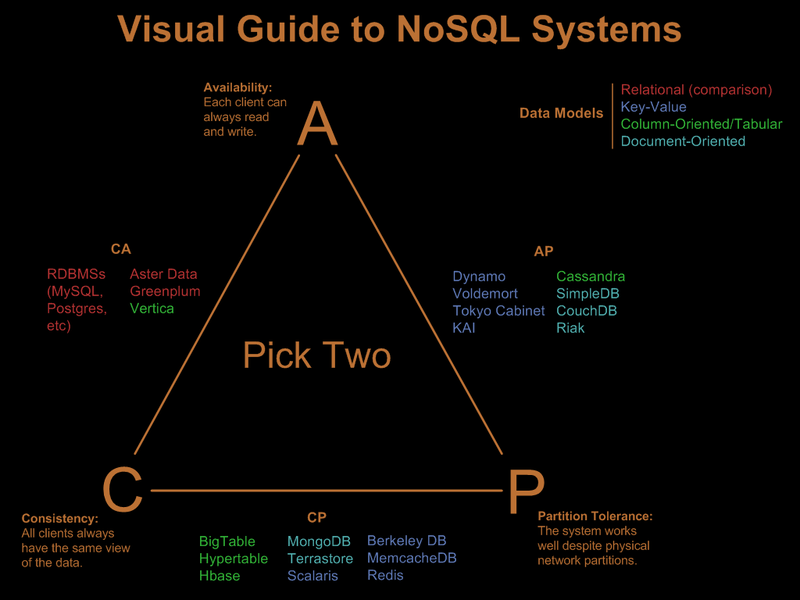
\includegraphics[scale=0.5]{images/cap_choice.png}


\subsubsection{Normalisation}
Normalisation is a way of structuring a relational database such that logical errors are minimized. 

\begin{lstlisting}[language=python]
from DB import DB


class DictOfSets:
    data = {}

    def addData(self, d):
        for row in d:
            if row[0] in self.data:
                self.data[row[0]].add(row[1])
            else:
                self.data[row[0]] = set([row[1]])

    def addVals(self, v):
        for row in v:
            if row[0] in self.data:
                self.data[row[0]].add(row[1])

    def addKeys(self, k):
        for key in k:
            if not key in self.data:
                self.data[key] = set()

        

class DBAbstr:
    host = '10.173.202.110'
    user = 'lesen'
    password = ''
    database = 'gkd_chemie'
    
    def doQuery(self, query):
        result = []
        with DB(self.host, self.user, self.password, self.database) as db:
            result = db.queryToArray(query)
        return result


class SetTable(DBAbstr):
    vals = []

    def __init__(self, tableName, key):
        self.tableName = tableName
        self.key = key

    def getVals(self):
        if self.vals:
            return self.vals
        query = "select {0} from {1} group by {0}".format(self.key, self.tableName)
        result = self.doQuery(query)
        self.vals = result
        return result


class RelTable(DBAbstr):
    leftVals = DictOfSets()
    rightVals = DictOfSets()

    def __init__(self, tableName, setA, translKeyA, setB, translKeyB):
        self.tableName = tableName
        self.setA = setA
        self.translKeyA = translKeyA
        self.setB = setB
        self.translKeyB = translKeyB

    def getLeftVals(self):
        if self.leftVals.data:
            return self.leftVals.data
        query  = "select a." + self.setA.key + ", c." + self.setB.key + " "
        query += "from " + self.setA.tableName + " as a "
        query += "left join " + self.tableName + " as b on b." + self.translKeyA + " = a." + self.setA.key + " "
        query += "left join " + self.setB.tableName + " as c on c." + self.setB.key + " = b." + self.translKeyB + " "
        query += "group by a." + self.setA.key + ", c." + self.setB.key
        result = self.doQuery(query)
        self.leftVals.addData(result)
        return result

    def getRightVals(self):
        if self.rightVals.data:
            return self.rightVals.data
        query  = "select a." + self.setB.key + ", c." + self.setA.key + " "
        query += "from " + self.setB.tableName + " as a "
        query += "left join " + self.tableName + " as b on b." + self.translKeyB + " = a." + self.setB.key + " "
        query += "left join " + self.setA.tableName + " as c on c." + self.setA.key + " = b." + self.translKeyA + " "
        query += "group by a." + self.setA.key + ", c." + self.setB.key
        result = self.doQuery(query)
        self.rightVals.addData(result)
        return result





class Relation:
    vals = DictOfSets()     # x  ->  f(x) = y
    invVals = DictOfSets()  # y  ->  f^-1(y) = x

    def __init__(self, setTableX, setTableY, relTable):
        self.setTableX = setTableX
        self.setTableY = setTableY
        self.relTable = relTable

    def checkTransitive(self):
        pass

    def checkBijective(self):
        """ One-to-one and onto """
        return self.checkSurjective and self.checkInjective

    def checkSurjective(self):
        """ Onto: For any y in Y, there is a x in X: y = f(x) """
        invValsData = self.getInvValsData()
        for y in invValsData:
            if len(invValsData[y]) == 0:
                return False
        return True

    def checkInjective(self):
        """  Ont-to-One: For any a, b in X: f(a) = f(b) => a = b """
        invValsData = self.getInvValsData()
        for y in invValsData:
            if len(invValsData[y]) > 1:
                return False
        return True
            

    def compose(self, rel2):
        pass


    def getValsData(self):
        if  self.vals.data:
            return self.vals.data
        xdata = self.setTableX.getVals()
        self.vals.addKeys(xdata)
        reldata = self.relTable.getLeftVals()
        self.vals.addVals(reldata)
        return self.vals.data


    def getInvValsData(self):
        if self.vals.data:
            return self.vals.data
        ydata = self.setTableY.getVals()
        self.invVals.addKeys(ydata)
        reldata = self.relTable.getRightVals()
        self.invVals.addVals(reldata)
        return self.invVals.data




if __name__ == "__main__":
    pnstMappen = SetTable('gkd_chemie.LIMNO_PNST_MAPPE', 'MAPPE_NR')
    messnetze = SetTable('gkd_chemie.LIMNO_SL_PNST_MAPPE_TYP', 'TYP_NR')
    pnstMappePnst = RelTable('gkd_chemie.LIMNO_ZT_PNST_MAPPE_PNST', pnstMappen, 'MAPPE_NR', messnetze, 'MN_NR')
    mappenMessnetzRel = Relation(pnstMappen, messnetze, pnstMappePnst)
    isInj = mappenMessnetzRel.checkInjective()
    isSur = mappenMessnetzRel.checkSurjective()
    print isInj
    print isSur

\end{lstlisting}



\subsection{Distributed cache: redis}

\section{Virtualisation}

\subsection{KVM/QEMU}


\subsection{Docker}

\section{Linux sound-stack}


All sound-in (microphone, jack/cinch aka line-in) and sound-out (loudspeakers, headphones) cables lead to your soundcard, which has the sole task of transforming analog sound signals to digital \inlinecode{short[]} arrays. The whole routing is done via the ALSA System. 
Because ALSA is a little complicated, linux has a layer on top of it. Two applications can be used as this top-layer: pulseaudio and jackd.  

\subsection{Audio Standards}

\paragraph{Raw audio} consists of \inlinecode{short[]} arrays containing raw amplitude data. 

\paragraph{Midi} comes in two forms: JACK-Midi and ALSA-Midi.

\subsection{Hardware}

Use \inlinecode{aplay -l} to list all your sound cards. 

\paragraph{PCH} is your actual soundcard. 

\paragraph{HDMI} is combined audio/video transport. Mostly used by monitors, but also shows up in \inlinecode{aplay -l} because it can carry sound as well. 

\subsection{Software}

There are different systems that controll your soundcards. 


\paragraph{ALSA} is linuxes standard sound routing mechanism. 

\paragraph{Portaudio} is an alternative to alsa that can also run on windows and mac. 

\paragraph{Jack} is a router that lets you plug one programs sound output into another programs sound input - or to the system's soundcard. 

\subsection{JACK}
Jack deserves its own section. 

\paragraph{Frames per period * periods per buffer} yields your buffer size. Big buffer means low CPU load, but large latency. Small buffer means small latency, but high CPU load. If the CPU load approaches 100\%, you'll hear \emph{xruns} (which stands for buffer-Under- or Over-run), that is clicking and artifacts caused by your CPU not being able to process buffer-batches on time. Jack displays CPU usage under the term \emph{DSP load} in qjackclt.

\paragraph{Realtime (RT)} mode requires your kernel to support realtime scheduling (called low-latency kernel). When that is given, jack will be given priority in memory and cpu over most other tasks. 
\section{Security}



\chapter{Programming languages}
\section{C}

\subsection{General theory}

\subsubsection{Memory allocation}
By default, memory is allocated statically to the stack. By using \inlinecode{malloc} and \inlinecode{free}, you can instead allocate memory dynamically on the heap.

\subsubsection{Threading}
Threads are created by making a copy of the orignal process.
Threads share the same memory with their parents.



% Please add the following required packages to your document preamble:
% \usepackage{booktabs}
% \usepackage{graphicx}
\begin{table}[ht]
\centering
\caption{Processes versus Threads}
\resizebox{\textwidth}{!}{%
\begin{tabular}{@{}lll@{}}
\toprule
              & Sub-Process                                                                                           & Thread                                                                                                                               \\ \midrule
Creation      & Copy of mother process                                                                                &                                                                                                                                      \\
Memory        & Own memory                                                                                            & Shared memory                                                                                                                        \\
Communication & \begin{tabular}[c]{@{}l@{}}Communicates with mother through \\ syscalls, pipes and files\end{tabular} & \begin{tabular}[c]{@{}l@{}}Can directly call methods of \\ mother process\end{tabular}                                               \\
Usecase       &                                                                                                       & \begin{tabular}[c]{@{}l@{}}Ideal if thread output to be processed \\ by mother process, \\ because no piping neccessary\end{tabular} \\ \bottomrule
\end{tabular}%
}
\end{table}


\begin{lstlisting}[language=c]
#include <stdio.h>
#include <stdlib.h>
#include <pthread.h>
 
// A normal C function that is executed as a thread 
// when its name is specified in pthread_create()
void *myThreadFun(void *vargp)
{
    sleep(1);
    printf("Printing GeeksQuiz from Thread \n");
    return NULL;
}
  
int main()
{
    pthread_t tid;
    printf("Before Thread\n");
    pthread_create(&tid, NULL, myThreadFun, NULL);
    pthread_join(tid, NULL);
    printf("After Thread\n");
    exit(0);
}
\end{lstlisting}

As mentioned above, all threads share data segment. Global and static variables are stored in data segment. Therefore, they are shared by all threads. The following example program demonstrates the same.

\begin{lstlisting}[language=c]
#include <stdio.h>
#include <stdlib.h>
#include <pthread.h>
 
// Let us create a global variable to change it in threads
int g = 0;
 
// The function to be executed by all threads
void *myThreadFun(void *vargp)
{
    // Store the value argument passed to this thread
    int *myid = (int *)vargp;
 
    // Let us create a static variable to observe its changes
    static int s = 0;
 
    // Change static and global variables
    ++s; ++g;
 
    // Print the argument, static and global variables
    printf("Thread ID: %d, Static: %d, Global: %d\n", *myid, ++s, ++g);
}
 
int main()
{
    int i;
    pthread_t tid;
 
    // Let us create three threads
    for (i = 0; i < 3; i++)
        pthread_create(&tid, NULL, myThreadFun, (void *)i);
 
    pthread_exit(NULL);
    return 0;
}
\end{lstlisting}

\begin{lstlisting}
gfg@ubuntu:~/$ gcc multithread.c -lpthread
gfg@ubuntu:~/$ ./a.out
Thread ID: 1, Static: 1, Global: 1
Thread ID: 0, Static: 2, Global: 2
Thread ID: 2, Static: 3, Global: 3
gfg@ubuntu:~/$ 
\end{lstlisting}

Please note that above is simple example to show how threads work. Accessing a global variable in a thread is generally a bad idea. What if thread 2 has priority over thread 1 and thread 1 needs to change the variable. In practice, if it is required to access global variable by multiple threads, then they should be accessed using a mutex.

\subsubsection{Getting data from C to another programm}


\begin{table}[ht]
\centering
\caption{Pipes versus sockets}
\begin{tabular}{ll}
\hline
Pipe                                                                                 & Socket                                                                               \\ \hline
Unidirectional                                                                       & Bidirectional                                                                        \\
Fifo                                                                                 &                                                                                      \\
\begin{tabular}[c]{@{}l@{}}Limited volume ($\sim$0.5 MB); \\ can block!\end{tabular} &                                                                                      \\
all in memory                                                                        & all in memory                                                                        \\
no protocol                                                                          & \begin{tabular}[c]{@{}l@{}}packets (UDP or TCP), \\ can go over network\end{tabular} \\
                                                                                     &                                                                                      \\ \hline
\end{tabular}
\end{table}

\paragraph{Per file}
Simplest, but also slowest because it involves disk i/o.

\paragraph{Per pipe or socket}
Faster than file-writing, because no disc i/o is involved. 
But still slow because data is chucked into packages that are wrapped in a rather verbose protocol.

\paragraph{Per JNI}
This should allow you to convert C-datastructures to Java-datastructures.




\subsection{Quirks and features you need to know}

\subsubsection{* syntax}

\begin{lstlisting}[language=c]
int a = 1; 
int * a_ptr = &a;
*a_ptr; // <--- yields 1
\end{lstlisting}

When assigning, * means: "make it a pointer". \\
When qerying, * means: "get the value behind the pointer". \\
\& always means: "get the address". \\ \\



\subsubsection{Pointer arithmetic}

Array indexing is actually a rather complex issue with a lot of syntactical sugar.

\begin{lstlisting}[language=c]
int arr[3] = {10, 20, 30};
arr[2] = 15;
\end{lstlisting}

\begin{itemize}
    \item $arr$ gets you the pointer to the first element in the array. In other words, we have $arr = \&arr[0]$
    \item $[2]$ adds to $arr$ the size of 2 ints. Thus we have $arr[2] = \&arr[0] + 2 * sizeof(int)$.
    \item Finally, the actal value behind the expression is adjusted when we assign the value of 15. Thus the expression reduces to 
            \begin{lstlisting}[language=c]
                *(&arr[0] + 2 * sizeof(int)) = 15;
            \end{lstlisting}
\end{itemize}


We can use array indexing to our advantage: with \emph{buffer overflow}s we can read arbitrary parts of the memory. 
Consider this simple example:

\begin{lstlisting}[language=c]
   int main () {
        int arr[3] = {1, 2, 3};
        int i;
        for(i=0; i < 100; i++){
                printf("%d th entry: location: %p value: %d \n", i, &arr[i], arr[i]);
        }
        return 0;
} 
\end{lstlisting}

Especially when creating arrays, we need to be aware of a few things: 
\begin{itemize}
	\item ... what is the current content of the accessed memory?
	\item ... is the accessed memory protected against overwriting by others?
\end{itemize}

\begin{lstlisting}[language=c]
#include<stdio.h>
#include <stdlib.h>  

int main() {

  const int size = 1000;
  //double data[size] = {2.1,2.1,2.1, 2.1, 2.1};   //<-- puts in vals; fills rest with zeros. This mem won't be overwritten. 
  //double data[size];      //<-- does not put in zeros - keeps whatever was in there before. This mem won't be overwritten.
  //double* data = (double*) malloc(size * sizeof(double));              //<-- puts in zeros. This mem won't be overwritten.
  //double* data;      //<-- does not put in zeros - keeps whatever was in there before. This mem can be overwritten by others! 
  for(int i = 0; i < size; i++) {
    double val = data[i];
    printf("val at %i: %f \n", i, val);
  }

  return 0; 
}
\end{lstlisting}
When we state that \emph{this mem won't be overwritten}, of course we exclude overwriting by buffer overflow. 

\subsubsection{Array decay: Functions can't accept arrays}

Functions never accept arrays, they only take pointers to the first element. This is known as array-decay.

\begin{lstlisting}[language=c]
int arr[3] = {1,2,3};
somefunct(arr); // <--- compiler turns this automatically into 
somefunct(&arr[0]);
\end{lstlisting}


\subsubsection{Array decay: Functions don't return arrays, either}

Functions return single values just fine, but arrays only by pointer. 
$arrFunct$ must save array on heap and return pointer to the heap.
The calling function must know the arrays size in advance or be given a struct with metainfo about the size.
The calling function must also later deallocate the array.

\begin{lstlisting}[language=c]
int * arrOnHeap(){
    int * arr_ptr = malloc( sizeof(int) * 3 );
    arr_ptr[0] = 10;
    arr_ptr[1] = 20;
    arr_ptr[2] = 30;
    return arr_ptr;
}

int * arr_ptr = arrOnHeap();
\end{lstlisting}


\subsubsection{Array syntax} 
Java and c have some weird differences in array initialisation. Consider array litterals: 
\begin{lstlisting}
int coeffs[5] = {1, 2, 3, 4, 5}; // c
int[] coeffs = {1, 2, 3, 4, 5};  // java
\end{lstlisting}
And also standard initialisation:
\begin{lstlisting}
int coeffs[5];   // c
int[] coeffs = new int[5]; // java
\end{lstlisting}


\subsubsection{Struct syntax}

There is a really important thing when creating struct-construction functions.
Consider the following code. 

\begin{lstlisting}[language=c]
typedef struct Island {
	char* name;
	char* opens;
	char* closes;
	struct Island* next;
} Island;


Island* island_create(char* name){
	Island* i = malloc(sizeof(Island));
	i->name = name;
	i->opens = "09:00";
	i->closes = "17:00";
	i->next = NULL;
	return i;
}

int main(){
    char* name;
    fgets(name, 80, stdin);
    Island* island1 = island_create(name);
    fgets(name, 80, stdin);
    Island* island2 = island_create(name);
    
    return 0;
}
\end{lstlisting}

You will find that the name of island1 equals that of island2!
The reason is that their names are just a reference to char* name in the main method. 
We need a safety measure inside the constructor to allocate a copy of the input string so that we can sure a new call to the constructor does not give us the same pointer again.

This code fixes the problem: 

\begin{lstlisting}[language=c]
Island* island_create(char* name){
    char* namec = strdup(name);
	Island* i = malloc(sizeof(Island));
	i->name = namec;
	i->opens = "09:00";
	i->closes = "17:00";
	i->next = NULL;
	return i;
}

void island_destroy(Island* i){
    free(i->name);
    free(i);
}
\end{lstlisting}



\subsubsection{Passing functions as variables}

This is our entry to functional programming in c.
A functionname is really just a pointer to the memory location where the function code is stored. So we can use the function name as a pointer.

Of course, functions have different types. That's why we can't just write 
\begin{lstlisting}[language=c]
function* f;
\end{lstlisting}

But instead must write:
\begin{lstlisting}[language=c]
char* (*reverseName)(char*);
\end{lstlisting}
Here, the first char* is the return type, whereas the second is the argument(-list) to the function. Let's see an example:


\begin{lstlisting}[language=c]
#include <stdio.h>
#include <stdlib.h>
#include <string.h>


int num_ads = 7;
char* ads[] = {
	"William: SBM GSOH likes sports, TV, dining",
	"Matt: SWM NS likes art, movies, theater",
	"Luis: SLM ND likes books, theater, art",
	"Mike: DWM DS likes trucks, sports and bieber",
	"Peter: SAM likes chess, working out and art",
	"Josh: SJM likes sports, movies and theater",
	"Jed: DBM likes theater, books and dining"
};


int likes_sport_not_bieber(char* ad){
	int hit = (strstr(ad, "sports") && !strstr(ad, "bieber"));
	return hit;
}

int likes_sports_or_workout(char* ad){
	int hit = (strstr(ad, "sports") || strstr(ad, "workout"));
	return hit;
}


void find(int (*match_fn)(char*)){
	puts("Search results:");
	puts("----------------------");

	int i;
	for(i=0; i < num_ads; i++){
		if(match_fn(ads[i])){
			printf("%s\n", ads[i]);
		}
	}

	puts("---------------------");
}

int main(){

	find(likes_sport_not_bieber);
	find(likes_sports_or_workout);

	return 0;

}

\end{lstlisting}


We should note some syntactic sugar here. 
Calling functions is usually done like this:
\begin{lstlisting}[language=c]
int a = somFunc(b);
\end{lstlisting}
But that's just shorthand for the actual code:
\begin{lstlisting}[language=c]
int a = (*somFunc)(b);
\end{lstlisting}

Also, passing functions as arguments really compiles down to:
\begin{lstlisting}[language=c]
find(&likes_sport_not_bieber);
\end{lstlisting}



\subsubsection{Strings end with a \textbackslash 0}

Thats why, when declaring an empty string, leave space for the \textbackslash 0 .

\begin{lstlisting}[language=c]
char word[3];
strcpy(word, "hi");
strlen(word); // <--- yields 2
sizeof(word); // <--- yields 3
\end{lstlisting}


\subsubsection{char[] does not equal char*}

\begin{lstlisting}[language=c]
char a[] = "hello";
char * b = "world";
\end{lstlisting}

$a$ is equal to: \boxed{H} \boxed{E} \boxed{L} \boxed{L} \boxed{O} \boxed{\backslash 0} \\
$b$ is equal to a \boxed{pointer} pointing to \boxed{W} \boxed{O} \boxed{R} \boxed{L} \boxed{D} \boxed{\backslash 0}




\subsubsection{Header files}

Header files are how we can expose only a subset of a file to main.c. Really they contain only the function signatures, not their implementation. In that way, c basically forces you to import \emph{everything} as an interface. 


\begin{lstlisting}[language=c,caption={main.c}]
#include <stdio.h>
#include "encrypt.h"

int main(){
    char msg[80];
    while(fgets(msg, 80, stdin)){
        encrypt(msg);
        printf("%s", msg);
    }
}
\end{lstlisting}


\begin{lstlisting}[language=c,caption={encrypt.h}]
void encrypt(char * msg);
\end{lstlisting}


\begin{lstlisting}[language=c,caption={encrypt.c}]
#include "encrypt.h"

void encrypt(char * msg) {
    char c;
    while(*msg){
        *msg = *msg ^ 31;
        msg++;
    }
}
\end{lstlisting}



\subsubsection{Building and Makefiles}
The building of an executable consists of compuiling and linking. 
\begin{itemize}
    \item \textbf{Compiling your own code} The compiler generates an object file from your sourcecode. An object-file is a compiled piece of code together with some meta-information on what kind of functions and structures it containes. 
    \item \textbf{Linking in libraries} After that, the include-directories are scanned for libraries that contain implementations of the header-files you included in your sourcecode. This phase is called linking. There are two ways you can link in external libraries.
    \begin{itemize}
        \item Static linking means that a copy of the library is added to the final executable at compile time. The executable can then be moved to another machine without worries, because all required libraries are placed inside the executable. Static libraries are usually written like this: \inlinecode{libXXX.a} and created with the \inlinecode{ar} program.
        \item  Alternatively, libraries can be linked in a dynamic way: that means that the executable will search for an appropriate library once it needs to call its functions, that is, at run time.  Shared/dynamic libraries are written like \inlinecode{libYYY.so} and created with \inlinecode{gcc -fPIC -c YYY.c && gcc -shared -o libYYY.so YYY.o}
        \item Both \inlinecode{.a} and \inlinecode{.so} libraries are included with the \inlinecode{-l} and \inlinecode{-L} commands. 
    \end{itemize}
\end{itemize}

Makefiles are how we knot together different parts of a c programm. It's really easiest to look at a specific example:

\begin{lstlisting}[language=bash]
# Includes are header files without a concrete implementation.
INCLUDES = -I/usr/include/mysql
# Libraries are object files. -L adds a directory of libraries, -l adds a single library. 
LIBS = -L/usr/lib/x86_64-linux-gnu -lmysqlclient -ljansson -pthread
WARNINGS = -Wall -Wextra

# Compilen
#   -c: compile (nur compile, nicht link!)
#   -g: fuer debugger

incl.o: incl.c incl.h
	gcc -g -c $(WARNINGS) $(INCLUDES) incl.c

jsn.o: jsn.c jsn.h incl.h
	gcc -g -c $(WARNINGS) $(INCLUDES) jsn.c

psql.o: psql.c jsn.h
	gcc -g -c $(WARNINGS) $(INCLUDES) psql.c

# Linken
# 	-o: object-file: name der fertigen binary
# 	-g: fuer debugger

psql: psql.o jsn.o incl.o
	gcc -g -o psql psql.o jsn.o incl.o $(LIBS)
	
clean: 
    rm *.o

all: psql clean
\end{lstlisting}
 
\paragraph{Includes} sind header files.
Option $-I$(dirname): hinzufügen dir zu Suchpfad für *.h files.
Im Gegensatz zu libs kann man bei incls nur dirs spezifizieren, nicht einzelne files. Dafür gibt es ja schon die \#include Direktive.

\paragraph{Libs} sind die den header files zu Grunde liegenden so files.
Option $-L$(dirname): hinzufügen dir zu Suchpfad für *.so files.
 	$-l$(libname): mit Einbinden einer lib.
 	$-pthread$: eine besondere Option; steht für -lpthread + definiere ein paar extra macros

Jansson ist ein externes Programm. Es muss erst ge-make-t werden (oder ge apt-get-tet), danach finden wir header per default in /usr/local/include und libs in /usr/local/lib

\subsubsection{Valgrind}
The $-g$ flags from the above makefile were actually meant for use in valgrind. 
Valgrind analyses your memory allocation. It does so by creating its own, fake versions of $malloc$ and $free$. Anytime these are called, valgrind does its bookkeeping to check if any allocated memory is left on the heap.

Analysing code with valgrind is easy. Just compile it and then run it like this:
\begin{lstlisting}
make all
valgrind -v --leak-check=full --show-leak-kinds=all --log-file=val.log ./psql input.json
\end{lstlisting}

\subsubsection{OpenMP}
OpenMP is a set of macros used for control-flow for threads. Think of automatically distributing your for-loop over threads.










\subsection{CMake and Autotools}
While make does a good job at automating the build of c-programs, all the commands you type there are platform dependent. For that reason, larger projects use more sophisticated buildsystems. They don't require less configuration (in fact, they usually require \emph{more} work) but they make it easier to create a build that will work on any platform. Usually they work by first scanning your environment and then creating makefiles for you. 

Working with these is not exactly pleasant. This section only contains a \emph{how-to} handle existing open-source projects that you have to get to compile somehow. 

We begin with autotools. 
\begin{itemize}
    \item \inlinecode{./configure}
    \item \inlinecode{make}
    \item \inlinecode{make install}
    \item Troubleshooting: most likely, some shared libraries will be missing. Find out which by calling \inlinecode{}
\end{itemize}




\subsection{Best practice}

The above quirks gave us a lot of points where we need to be careful in c. 
For that reason, we should adhere to some best practices to make coding as save as possible.

\paragraph{Only expose top and lowest layer, not internals} Datastructures in C tend to be actual data wrapped in structs wrapped in structs wrapped in structs. The highest level struct should only expose data, not any intermediate structs. This way, a user only needs to know the api for the highest level struct and the data itself. Also, every struct should manage its own and only its own memory.

\paragraph{Handling unknown datatype elements} Your datastructures will usually contain elements of a type unknown to you. That is not really a problem, because you can reference them using a void*. But how about creating and destroying those unknown elements? Well, here we can use c's functional programming skills: just add to the datastructure a function for creating and one for destroying the element.

\paragraph{Never leave a pointer unassigned} You can create a pointer without having it point anywhere in particular: \inlinecode{int* apt;}. But what if later in your code you want to check if that pointer has been pointed to an int yet? \inlinecode{apt} is initially just going to point to some random location. This means that you cannot check \inlinecode{if(apt == NULL)}, because it's never going to be 0! For this reason, even if you don't want \inlinecode{apt} to point to anything yet, at least make sure it points to \inlinecode{NULL}. So always create pointers with \inlinecode{int* apt = NULL;}

\section{C++}

C++ is the best compromise between raw power and versatility. Fortran is faster in large matrix-operations, but lacks the abstraction of OOP and any multi-media support. Java is even better abstracted and has an unbeatable ecosystem with modules for everything, but slower. 



\subsection{Some weird syntax and new concepts}
Contrary to garbage-collected languages, where you only need to care about who knows about a given object, in cpp you also net to worry about where that object lives. 

\subsubsection{References}
Refences are really just syntactic sugar around pointers. It's still useful to know a few of their basic properties, since they are intended to help you avoid errors in memory management. 

Using pointers, to mutate an object you need to use pointer syntax for any operation on the object. This is known as dereferencing: using \inlinecode{*vpt} and \inlinecode{vpt->}.
\begin{lstlisting}[language=c++]
void foo(Vec* vpt){
    vpt->increment(1);
}

Vec vec = Vec();
foo(&vec);
\end{lstlisting}

Using references we can act as if the actual object and not just a pointer to it was in the function scope.
\begin{lstlisting}[language=c++]
void foo(Vec& v){
    v.increment(1);
}

Vec vec = Vec();
foo(vec);
\end{lstlisting}

Syntax: 
\begin{lstlisting}[language=c++]
int i = 3;
int* i_ptr = &i;
int& i_ref = i;
\end{lstlisting}

There are a few more noteworthy properties of references that are intended to make your life easier:
\begin{itemize}
    \item A pointer may point to nothing\footnote{However, this is very bad practice. Always initialize your free pointers to null using \inlinecode{int* ap = nullptr;}} - you may write \inlinecode{int* nullpt;}. A reference however mustn't do that. This will not compile: \inlinecode{int& nullrf;}.
    \item You can point a pointer to a new object, but a reference allways points to the same object. This will have \inlinecode{ap} point to \inlinecode{b}: 
    \begin{lstlisting}
    int a = 1; 
    int b = 2; 
    int& ar = a; 
    ar = b;
    \end{lstlisting}
    This, however, will overwrite \inlinecode{a}: 
    \begin{lstlisting}
    int a = 1; 
    int b = 2; 
    int& ar = a; 
    ar = b;
    cout << a << endl;  // yields 2 (!)
    \end{lstlisting}
\end{itemize}
\subsubsection{Const keyword}
Sometimes you want immutability; in cpp probably even more than in other languages, for security reasons. That is what the \inlinecode{const} keyword is there for. In most cases, you'll use this keyword when a function is passed some objects that it mustn't alter. Passing the objects as consts guarantees that the function has no sideeffects on the objects. 
\begin{lstlisting}[language=c++]
bool isEqual(const Vec & v1, const Vec & v2) {
    bool eq = false;
    if( v1.x == v2.x && v1.y == v2.y ){
        eq = true;
    }
    return eq;
}
\end{lstlisting}

Of course, we could also have avoided side-effects on v1 and v2 by just passing by value, because then the function would have only altered it's own copies of v1 and v2. But creating those copies is a costly operation, so we're cheeper of by passing by reference and using const to achieve immutability. 

Unfortunately, \inlinecode{const} has some weird syntax rules. The trick is in figuring out whether a value or a pointer to a value is to be constant. The rule is that \inlinecode{const} allways applies to the keyword to it's left. If there is nothing on the left, it applies to the keyword on the right. 
\begin{lstlisting}
const int a = 1;                // a constant integer
const int* a_ptr = nullptr;     // a variable pointer to a constant integer
int const* a_ptr;               // a variable pointer to a constant integer
int * const a_ptr;              // a constant pointer to a variable integer (you will rarely need this)
\end{lstlisting}




\subsection{Object orientation}
Here is a simple example of the class-syntax in cpp.

\begin{lstlisting}[language=c++]
#include <iostream>
#include <string>

using std::string;

class Robot {
  
  private:
    string name;
    int hitpoints;
  
  public:
    Robot(string n, int hp) : name(n), hitpoints(hp){
      std::cout << "Created " << name << " with " << hitpoints << " health" << std::endl;
    }
    
    void hit(Robot* other){
      other->takeHit(10);
    }
    
    void takeHit(int strength){
      hitpoints -= strength;
      std::cout << name << " now has " << hitpoints << " health" << std::endl;
    }
    
    ~Robot(){
      std::cout << name << " destroyed." << std::endl;
    }
};

int main() {
  Robot b("Bender", 100);
  Robot v("Vender", 100);
  b.hit(&v);
  return 0;
}
\end{lstlisting}

From this basic example we can already note a few important points.


\paragraph{Constructors} cpp knows \emph{three} ways of creating objects: 
\begin{itemize}
    \item The default constructor \inlinecode{Robot b("Bender", 100);} is what you should usually make use of. 
    \item Construction by assignment operator \inlinecode{Robot b = Robot("Bender", 100);} requires a functioning implementation of the assignment operator \inlinecode{Robot& operator=(const Robot& otherRobot)\{ ... return *this;\}}. If this isn't provided, the compiler generates one automatically. 
    \item Construction by copying an existing instance \inlinecode{Robot b("Bender", 100); Robot v(b);} requires a functioning implementation of the copy constructor \inlinecode{Robot(const Robot& otherRobot)}. If this isn't provided, the compiler generates one automatically. 
\end{itemize}

\paragraph{Constructors as objects or as pointers} Objects can be constructed as objects or as pointers to objects. 

Construction as object: 
\begin{lstlisting}[language=c++]
Particle p = Particle(20, 30);
p.move();
\end{lstlisting}
Here the object is automatically destroyed once it goes out of scope. Note the missing \inlinecode{new} keyword.

Construction as pointer: 
\begin{lstlisting}[language=c++]
Particle* p = new Particle(20, 30);
p->move();
delete p;
\end{lstlisting}
Here, the object survives until you manually call \inlinecode{delete p}.

Whenever possible, you should prefer the first method. However, there are some situations when it makes sense to use pointers: 

\begin{itemize}
    \item when the object is returned from a function (or any other situation where the object needs to outlive its scope)
    \item When you're passing the object to a function and you want that function to change the object and not just a copy of the object. 
\end{itemize}



\paragraph{Initialisation} Note also this important difference. In java, when you write \inlinecode{Perticle p;} this creates an uninitialized reference. In c++ however, this same command already does the initialisation by calling the default constructor.



\subsubsection{Operator overloading}
You can override any operator, as long as the operation makes use of at least one custom datatype. 

\begin{lstlisting}[language=c++]
#include <iostream>
#include <string>

using std::string;

class Vector {
  public:
    int x;
    int y;
    int z;
    Vector(int _x, int _y, int _z) : x(_x), y(_y), z(_z) {
      std::cout << "Created: [" << x << "," << y << "," << z << "]" << std::endl;
    }
    ~Vector(){
      std::cout << "Going out of scope: [" << x << "," << y << "," << z << "]" << std::endl;
    }
};


Vector operator+(Vector const & v1, Vector const & v2) {
  int x = v1.x + v2.x;
  int y = v1.y + v2.y;
  int z = v1.z + v2.z;
  Vector v3 = Vector(x, y, z);
  return v3;
}

int main() {
  
  Vector a = Vector(1, 2, 3);
  Vector b = Vector(2, 3, 4);
  Vector c = a + b;
  return 0;
}
\end{lstlisting}

\paragraph{A very special case: assignment operator} The assignment operator is a very special case. It is only allowed to be defined inside a class. But it is very useful to get an insight into what happens when you do an assignment in c++.
example with overwriting an object

From this we learn a very important lesson about the assignment operator. When one object is assigned to another, a copy of the actual values is made. In Java, copying an object variable merely establishes a second reference to the object. Copying a C++ object is just like calling clone in Java. Modifying the copy does not change the original.
\begin{lstlisting}[language=c++]
Point q = p; /* copies p into q */
q.move(1, 1); /* moves q but not p */
\end{lstlisting}


\paragraph{Assignment by copying versus assignment by moving} The last paragraph was not absolutely honest with you: you can force cpp to move an object instead of copying it when doing an assignment. 
ex with std::move



\subsubsection{Rule of three}
The rule of three states that if you write a custom constructor or destructor, you're also going to need a custom copy-constructor and a custom assignment-operator. The rule basically comes down to this: if you do any memory management during construction, you will also do memory management during copying and during destruction. The compiler cannot guess that memory management for you, so you need to specify it yourself. 

\begin{lstlisting}[language=c++]
class Ball {
    private:
        int xpos;
		int ypos;
		int xvel;
		int yvel;

    public:
        Ball(int x, int y) : xpos(x), ypos(y) {   // Standard constructor
        	std::cout << "ball created" << std::endl;
        }
        		
        ~Ball() {
        	std::cout << "ball deleted" << std::endl;
        }
        
        Ball(const Ball&) = delete;    // Copy constructor (note that argument has no name when using delete)
		Ball& operator=(const Ball&) = delete;     // Assignment operator (note that argument has no name when using delete)
        
        void move() {
        	xpos += xvel;
        	ypos += yvel;
        }
        		
        void push(int dvx, int dvy) {
        	xvel += dvx;
        	yvel += dvy;
        }
};
\end{lstlisting}



\subsubsection{Smart pointers}
With a \inlinecode{unique_ptr} you can make sure that only one object, the owner of the pointer, can access the value behind the pointer. Consider this epic tale of a king and his magic sword: 
\begin{lstlisting}[language=c++]
#include <iostream>
#include <string>
#include <memory>

using std::string;

class Weapon {
  private:
    string name;
  
  public:
    Weapon(string n = "rusty sword") : name(n) {
    
    }
    
    ~Weapon(){
      std::cout << name << " destroyed" << std::endl;
    }
    
    string getName() {
      return name;
    }
};

class Hero {
  private:
    string name;
    Weapon* weapon_ptr;
  
  public:
    Hero(string n) : name(n), weapon_ptr(nullptr) {}
    
    ~Hero(){
      if(weapon_ptr != nullptr){ 
        std::cout << name << " now destroying " << weapon_ptr->getName() << std::endl;
        delete weapon_ptr;
      }
      std::cout << name << " destroyed." << std::endl;
    }
    
    void pickUpWeapon(Weapon* w) {
      if(weapon_ptr != nullptr) delete weapon_ptr;
      weapon_ptr = w;
    }
    
    string describe() {
      if(weapon_ptr != nullptr){
        return name + " now swings " + weapon_ptr->getName();
      } else {
        return name + " now swings his bare hands";
      }
    }
};

Weapon* blacksmithForge(string name){
  Weapon* wp = new Weapon(name);
  return wp;
}


int main() {
  
  Hero arthur = Hero("Arthur");
  Hero mordred = Hero("Mordred");
  Weapon* excalibur = blacksmithForge("Excalibur");
  
  std::cout << arthur.describe() << std::endl;
  arthur.pickUpWeapon(excalibur);
  std::cout << arthur.describe() << std::endl;
  mordred.pickUpWeapon(excalibur);
  std::cout << mordred.describe() << std::endl;
  std::cout << "Everything going out of scope." << std::endl;
  
  return 0;
}
\end{lstlisting}

Note how Mordred has snatched away Arthurs sword. When mordred dies, he takes Excalibur with him into the grave. When Arthur dies, he tries to do the same, but has to find that the sword he thought he had was no longer there. We can fix this problem by using \inlinecode{unique_ptr}'s:

\begin{lstlisting}[language=c++]
#include <iostream>
#include <string>
#include <memory>

using std::string;

class Weapon {
  private:
    string name;
  
  public:
    Weapon(string n = "rusty sword") : name(n) {};
    
    string getName() {
      return name;
    }
};

class Hero {
  private:
    string name;
    std::unique_ptr<Weapon> weapon_ptr;
  
  public:
    Hero(string n) : name(n), weapon_ptr(new Weapon(n + "'s bare hands")) {}
    
    void pickUpWeapon(std::unique_ptr<Weapon> w) {
      if(!w){
        std::cout << "Nothing to pick up." << std::endl;
        return;
      }
      weapon_ptr = std::move(w);
    }
    
    string describe() {
        return name + " now swings " + weapon_ptr->getName();
    }
};

std::unique_ptr<Weapon> blacksmithForge(string name){
  std::unique_ptr<Weapon> wp(new Weapon(name));
  return wp;
}


int main() {
  
  Hero arthur = Hero("Arthur");
  Hero mordred = Hero("Mordred");
  std::unique_ptr<Weapon> excalibur = blacksmithForge("Excalibur");
  
  std::cout << arthur.describe() << std::endl;
  arthur.pickUpWeapon(std::move(excalibur));
  std::cout << arthur.describe() << std::endl;
  
  std::cout << "Mordred now tries to snatch Excalibur." << std::endl;
  mordred.pickUpWeapon(std::move(excalibur));
  std::cout << mordred.describe() << std::endl;
  

  std::cout << "Everything going out of scope." << std::endl;
  
  return 0;
}
\end{lstlisting}




\subsubsection{Ownership: unique, shared and weak pointers}
Let us explain in a bit more detail what a smart pointer is. Really, it i just a class encapsulating a raw pointer. The idea is that by wrapping a pointer in a class, we can have the class object be allocated on the stack and have it free the memory behind the pointer when the object is destroyed. This way, you don't have to manually delete a pointer.

\begin{lstlisting}[language=c++]
class SmartPointer{
    private:
        T* ptr;
    public:
        SmartPointer(T* p){
            ptr = p;
        }
        ~SmartPointer(){
            free(ptr);
        }
}
\end{lstlisting}

In this example, we allocate Excalibur on the heap. But because we're using smart pointers, we never have to clean up memory manually:
\begin{lstlisting}[language=c++]
#include <iostream>
#include <memory>

using std::string;

class Weapon{
  private:
    string name;
  public:
    Weapon(string n) : name(n){}
    string getName(){
      return name;
    }
    ~Weapon(){
      std::cout << name << " is being destroyed" << std::endl;
    }
};

class Hero{
  private:
    string name;
    std::unique_ptr<Weapon> weapon;
  public:
    Hero(string n) : name(n), weapon(new Weapon("rusty sword")) {}
    void pickWeapon(std::unique_ptr<Weapon> w){
      std::cout << name << " picked up " << w->getName() << std::endl;
      weapon = std::move(w);
      std::cout << weapon->getName()  << " is now on " << name << std::endl;
    }
    ~Hero(){
      std::cout << name << " is being destroyed" << std::endl;
    }
};

int main() {
  
  Hero arthur("Arthur");
  std::unique_ptr<Weapon> w(new Weapon("Excalibur"));
  arthur.pickWeapon(std::move(w));
  
  return 0;
}
\end{lstlisting}

Note how we used \inlinecode{move(w)} to overwrite \inlinecode{weapon}. What happens here is this: In the main-scope, the \inlinecode{w}'s internal pointer to Excalibur is replaced by a \inlinecode{nullptr}. Any further attempt of accessing \inlinecode{w} will cause a runtime-error. Inside the \inlinecode{pickWeapon} method, the old smartpointer to the rusty sword is destroyed, causing the sword itself to be free'd.  
We could'nt have used \inlinecode{weapon = w;}; that would have caused an error (because \inlinecode{unique_ptr}'s copy-assignment method is delted). This is deliberate: we don't want copies of a unique pointer to exist. We want a unique pointer to only ever exist in one place (in this case: first in the \inlinecode{main} function, later in the \inlinecode{arthur} instance), so that the memory behind the pointer can only get freed once (in this case: when \inlinecode{arthur} is destroyed).

Generally, we can proclaim the following rules:
\begin{itemize}
    \item When you're given a reference, someone else will clean up the original. 
    \item When you're given a unique pointer, you are now the sole owner of the smartpointer. If you move the pointer, it will go out of scope once you do; if you don't, it will go out of scope once your method ends. Passing a unique pointer to a method that doesn't move the pointer means destroying the object! To pass a unique pointer to a method without it being destroyed or moved, don't pass the unique pointer, pass a \inlinecode{unique_ptr<T> const &}.
    \item When you're given a shared pointer, ... . Shared pointers use reference counting just like the java garbage collector.  
\end{itemize}
There are a lot more useful tips \hyperlink{https://herbsutter.com/2013/06/05/gotw-91-solution-smart-pointer-parameters/}{here} and \hyperlink{https://stackoverflow.com/questions/8114276/how-do-i-pass-a-unique-ptr-argument-to-a-constructor-or-a-function}{here}.


\paragraph{Using ownership wisely} Based on this, we can define different ownership strategies depending on whether an object is a value-object or an id-object. 


\subsection{Templates}
Templates are like java generics. 

\subsubsection{Function template}

\begin{lstlisting}[language=c++]
#include <iostream>
#include <string>

using namespace std;

template <typename T>
inline T const& Max (T const& a, T const& b) { 
   return a < b ? b:a; 
}

int main () {
   int i = 39;
   int j = 20;
   cout << "Max(i, j): " << Max(i, j) << endl; 

   double f1 = 13.5; 
   double f2 = 20.7; 
   cout << "Max(f1, f2): " << Max(f1, f2) << endl; 

   string s1 = "Hello"; 
   string s2 = "World"; 
   cout << "Max(s1, s2): " << Max(s1, s2) << endl; 

   return 0;
}
\end{lstlisting}


\subsubsection{Class template}


\subsection{Threading} 
Comared to c's posix threads, c++ has somewhat simplified it's core threading library. 
\begin{lstlisting}[language=c++]
#include <iostream>
#include <thread>

void threadFunc(int i) {
  for(int j = 0; j < 100; j++){
    std::cout << "hi! this is operation " << j <<" from thread nr " << i << std::endl;
  }
}

int main(){
  std::thread threads[10];
  
  for(int i = 0; i<10; i++){
    threads[i] = std::thread(threadFunc, i);
  }
  
  for(int i = 0; i<10; i++){
    threads[i].join();
  }
  
  return 0;
}
\end{lstlisting}
You can avoid some of the above problem using barriers in your code (\inlinecode{std::mutex}) which will let you synchronize the way a group of threads share a resource.

\subsection{SDL}

Sdl is even simpler than openframeworks, but lacks some of of's more advanced features. However, to get started with simple programs, it seems ideal. 

\subsubsection{setup}


\subsection{OpenFrameworks}

This is the C++ equivalent of processing. There are a few basics you need to be aware of. 

\begin{itemize}
    \item Your \inlinecode{ofApp} extends \inlinecode{ofBasicApp} which exposes a bunch of virtual methods that you may or may not implement to hook into their functionality. 
    \item \inlinecode{ofApp}'s are threaded, so you might need mutex'es to synchronise audio and video, for example. 
\end{itemize}


\subsubsection{of native fuctions}


\paragraph{audioReceived}

\paragraph{ofThread}

\paragraph{ofMutex} This has all other threads wait with outputting anything until the action inside the lock is completed. 
\begin{lstlisting}
ofMutex soundMutex;
soundMutex.lock();
// do stuff here
soundMutex.unlock();
\end{lstlisting}

\section{Java}

We tend to use java when we want to create enterprise level software. The whole development-experience is way different from c. While in c you control every detail of the program, a java-app has you reuse as many standardized components as possible. There are layers upon layers of abstraction. Usually, there is some way to build on top of a framework, leaving you to only fill out a few xml-configurations and implement a few skeleton-beans with loads of annotations.


\subsection{General}

\subsubsection{Basic theory}

\subsubsection{Environment variables} 

First things first, to find out if you're using a 64 bit version of the jdk, just execute
\begin{lstlisting}
java -d64 -version
\end{lstlisting}
This will throw an error if your version is not made for 64 bit. 

There are a few environment variables that you should know about: 
\begin{itemize}
    \item PATH: Sys looks for exes here. Your JAVA\_HOME/bin should be part of PATH
    \item CLASSPATH: Java looks for code here
    \item JAVA\_HOME: location jdk (example: /usr/lib/jvm/java-7-openjdk-amd64/bin)
    \item JRE\_HOME: location jre (example: /usr/lib/jvm/java-7-openjdk-amd64/jre/bin)
\end{itemize}

The most important setting for the JVM is the heap size: how much memory will we allocate to the java-process? There are two settings: 
\begin{itemize}
    \item \inlinecode{-Xms<size>} - Set initial Java heap size
    \item \inlinecode{-Xmx<size>} - Set maximum Java heap size
\end{itemize}
These are either set in .... or used directly when invoking java with \inlinecode{java -Xms512m -Xmx1024m JavaApp}.

You can display the default settings like this: 
\begin{lstlisting}
$ java -XX:+PrintFlagsFinal -version | grep -iE 'HeapSize|PermSize|ThreadStackSize'

    uintx InitialHeapSize                          := 64781184        {product}
    uintx MaxHeapSize                              := 1038090240      {product}
    uintx PermSize                                  = 21757952        {pd product}
    uintx MaxPermSize                               = 174063616       {pd product}
     intx ThreadStackSize                           = 1024            {pd product}
java version "1.7.0_51"
OpenJDK Runtime Environment (IcedTea 2.4.4) (7u51-2.4.4-0ubuntu0.13.10.1)
OpenJDK 64-Bit Server VM (build 24.45-b08, mixed mode)
\end{lstlisting}

Here are some suggested values: 
\begin{itemize}
    \item Heap = -Xms512m -Xmx1024m
    \item PermGen = -XX:PermSize=64m -XX:MaxPermSize=128m
    \item Thread = -Xss512k
\end{itemize}


\subsection{Maven}

Maven is a build- and dependency-resolution tool. Building eg. webprojects with maven is encouraged, also because maven takes away buildsteps from your IDE. Relying on maven instead of an IDE to do your building then makes your builds portable between different developement environments. 

Maven can initialise a project structure for you from the command-line:
\begin{verbatim}
mvn archetype:generate -DarchetypeArtifactId=maven-archetype-quickstart
\end{verbatim} 
It will then ask you all further neccessary information. 

\paragraph{cli syntax} 
The syntax generally consists of mvn [lifecycle]:[phase]:[args]

\begin{lstlisting}[language=bash]
mvn default:package
mvn [lifecyle]:[phase]
mvn default:package:help
\end{lstlisting}
		
		
\paragraph{build lifecyles} 

Maven has a quite hierarchical structure to it. 

\begin{itemize}
    \item lifecycles: default (compiling et al), clean (remove artifacts), site (create documentation). Plugins might add further lifecycles. 
    \begin{itemize}
        \item phases : default build lifecycle consists of several phases: validate, compile, test, package, verify, install, deploy
        \begin{itemize}
            \item goals: each phase executes one or more goals. these are the actual code instuctions. 
        \end{itemize}
        \item profiles : here we can adjust some environment settings. should never really be neccessary.
    \end{itemize}
    \item plugin: a set of extra goals for maven. plugins might even define whole new lifecycles like 'mvn jetty:run', or hook into the build cycle to generate code from xml like cxf does. 
    \begin{itemize}
        \item mojo : maven pojo. a class representing an executable goal
        \item configuration of plugins. executions : specifies how the mojo should be executed; ie in which phase of the maven build-lifecycle
    \end{itemize}
\end{itemize}

\paragraph{Directory structure}
Everything that you put under \emph{src/main/resources} during development will be put under the root-directory on compilation. Same thing holds for the contents of \emph{src/test/resources}: they will be on the root path during execution of tests. So, when using relative paths, \emph{src/*/resources/} must be omitted.


\paragraph{Custom archetypes}

\paragraph{Custom plugins}




\subsection{Threading}

Java was designed to make threading easy (though, contrary to clojure, it was not designed to make threading \emph{save}). 

\paragraph{Basic threading with shared data} is the simplest, but somewhat dangerous method. 
\begin{lstlisting}[language=java]
public class Main {
	
	public static void main(String[] args) throws InterruptedException {
		
		LinkedList<Integer> sharedData = new LinkedList<Integer>();
		Producer p = new Producer(sharedData);
		Consumer c = new Consumer(sharedData);
		p.start();
		Thread.sleep(1000);
		c.start();
		
	}

}
\end{lstlisting}
\begin{lstlisting}[language=java]
public class Producer extends Thread {

	private LinkedList<Integer> sharedData;

	public Producer(LinkedList<Integer> sharedData) {
		this.sharedData = sharedData;
	}
	
	@Override
	public void run() {
		Random r = new Random();
		while(true) {
			try {
			    Integer i = r.nextInt(5);
				Thread.sleep(100 * i);
    			sharedData.add(i);
    			System.out.println("Producer just added " + i + " to the shared data.");
    			System.out.println("Data now looks like this: " + sharedData.toString());
			} catch (InterruptedException e) {
				e.printStackTrace();
			}
		}
	}
}
\end{lstlisting}
\begin{lstlisting}[language=java]
public class Consumer extends Thread {

	private LinkedList<Integer> sharedData;

	public Consumer(LinkedList<Integer> sharedData) {
		this.sharedData = sharedData;
	}
	
	@Override
	public void run() {
		Random r = new Random();
		while(true) {
			try {
				Thread.sleep(100 * r.nextInt(5));
				i = sharedData.removeFirst();
    			System.out.println("Consumer just took " + i + " from the shared data.");
    			System.out.println("Data now looks like this: " + sharedData.toString());
			} catch (InterruptedException e) {
				e.printStackTrace();
			}
		}
	}
	
}
\end{lstlisting}

This results in an output like this: 
\begin{lstlisting}
Producer just added 3 to the shared data.
Data now looks like this: [0, 0, 3]
Consumer just took 0 from the shared data.
Data now looks like this: [0, 3]
Consumer just took 0 from the shared data.
Data now looks like this: [3]
Consumer just took 3 from the shared data.
Data now looks like this: []
Exception in thread "Thread-1" java.util.NoSuchElementException
	at java.util.LinkedList.removeFirst(LinkedList.java:270)
	at threadingStuff.Consumer.run(Consumer.java:20)
\end{lstlisting}

Notice how at some point the consumer overtook the producer, leading to a \verb NoSuchElementException  . We can use signaling to handle this kind of situation: 
\begin{itemize}
    \item \inlinecode{wait()}
    \item \inlinecode{notify()}
\end{itemize}

Alternatively, a blocking queue would automatically handle such a case by just blocking the consumer until data is available again.

\paragraph{Using a blocking queue} makes sense when 
\begin{itemize}
    \item you need protection from \verb NoSuchElementException  .
    \item it is ok for the consumer to sometimes be blocked while waiting for data to arrive.
\end{itemize}
\begin{lstlisting}[language=java]
public class Main {
	
	public static void main(String[] args) throws InterruptedException {
		
		ArrayBlockingQueue<Integer> sharedData = new ArrayBlockingQueue<Integer>(100);
		Producer p = new Producer(sharedData);
		Consumer c = new Consumer(sharedData);
		p.start();
		Thread.sleep(1000);
		c.start();
		
	}

}
\end{lstlisting}
\begin{lstlisting}[language=java]
public class Producer extends Thread {

	private ArrayBlockingQueue<Integer> sharedData;

	public Producer(ArrayBlockingQueue<Integer> sharedData) {
		this.sharedData = sharedData;
	}
	
	@Override
	public void run() {
		Random r = new Random();
		while(true) {
			try {
				Integer i = r.nextInt(5);
				Thread.sleep(100 * i);
				sharedData.put(i);
				System.out.println("Producer just added " + " to the shared data.");
				System.out.println("Data now looks like this: " + sharedData.toString());
			} catch (InterruptedException e) {
				e.printStackTrace();
			}
		}
	}
}
\end{lstlisting}
\begin{lstlisting}[language=java]
public class Consumer extends Thread {

	private ArrayBlockingQueue<Integer> sharedData;

	public Consumer(ArrayBlockingQueue<Integer> sharedData) {
		this.sharedData = sharedData;
	}
	
	@Override
	public void run() {
		Random r = new Random();
		Integer i;
		while(true) {
			i = null;
			try {
				Thread.sleep(100 * r.nextInt(5));
				i = sharedData.take();
				System.out.println("Consumer just took " + i + " from the shared data.");
				System.out.println("Data now looks like this: " + sharedData.toString());
			} catch (InterruptedException e) {
				e.printStackTrace();
			}
		}
	}
	
}
\end{lstlisting}

This results in an output like this: 
\begin{lstlisting}
Producer just added 3 to the shared data.
Data now looks like this: [0, 0, 3]
Consumer just took 0 from the shared data.
Data now looks like this: [0, 3]
Consumer just took 0 from the shared data.
Data now looks like this: [3]
Consumer just took 3 from the shared data.
Data now looks like this: []     // <------ no exception thrown here! Consumer just has to wait. 
Producer just added 3 to the shared data.
Data now looks like this: [3]
Producer just added 4 to the shared data.
Data now looks like this: [3, 4]
\end{lstlisting}


\paragraph{Using a pipe} makes only sense under very specific conditions. A pipe is optimized for serialized in- and output, so you'd first have to serialize and then deserialize anything that has to pass through the pipe. Also, a pipe can always only exist between exactly two threads, no more. 

\paragraph{Using an executor service} makes sense when ...

\paragraph{Calling another thread's mehtods} is actually possible without much ado: 
\begin{lstlisting}[language=java]
class Main {
    public static void main() {
        RT rt = new RT();
        rt.start();
        rt.updateV(3);
    }
}
\end{lstlisting}
\begin{lstlisting}[language=java]
class RT extends Thread {
    private int v; 
    
    public RT() {
        v = 1;
    }

    public void run() {
        while(true){
            Thread ct = Thread.currentThread();
            String name = ct.getName();
            System.out.println("Method run() being executed on " + name);
            System.out.println("v now is: " + v);
        }
    }
    
    public void updateV(int newV) {
        Thread ct = Thread.currentThread();
        String name = ct.getName();
        System.out.println("Method updateV() being executed on " + name);
        v = newV;
    }
}
\end{lstlisting}
%The main thread can call \inlinecode{accessibleMethod()} without problems. The method will be executed on the \inlinecode{RT}-thread. The execution of that method temporarily halts the execution of the \inlinecode{run()} method. Using \inlinecode{getState()} you will see that the thread is in the \inlinecode{BLOCKED}  state while the \inlinecode{accessibleMethod()} is being executed. 
A thread's public methods may be called from anywhere. So the main thread can call \inlinecode{accessibleMethod()} without problems.  However, the execution of that public method will than take place on the calling thread - in that case, the main thread. You can verify this by sparkling your code with a few \inlinecode{Thread.currentThread().getName()} calls. But the called method may still manipulate a variable that is private to the called thread; so the main thread may manipulate \inlinecode{v}. This is possible because threads share the same memory base. 

\subsection{Functional programming}

Java 8 exposes a few new Classes that can be used as functions. 
\begin{itemize}
    \item \inlinecode{Function<Integer,Integer> add3 = a -> a + 3;}
    \item \inlinecode{BiFunction<Integer, Integer, Integer> add = (a, b) -> a + b;}
    \item \inlinecode{Predicate<Integer> isEven = a -> a\%2 == 0;} A predicate always returns a boolean.
    \item \inlinecode{Consumer<Book> storeAway = b -> b.save();} A consumer returns void. 
\end{itemize}

\begin{lstlisting}[language=java]

public static void main() {
    BiFunction<Integer, Integer, Integer> add = (a, b) -> a + b;
    BiFunction<Integer, Integer, Integer> sub = (a, b) -> a - b;
    Integer result1 = compute(add, 3, 4);
    Integer result2 = compute(sub, 3, 4);
}

public static Integer compute(BiFunction<Integer, Integer, Integer> function, Integer a, Integer b) {
    return function.apply(a, b);
}
\end{lstlisting}

These functions could also have been passed anonymously: 
\begin{lstlisting}[language=java]

public static void main() {
    Integer result1 = compute((a, b) -> a + b, 3, 4);
    Integer result2 = compute((a, b) -> a - b, 3, 4);
}

public static Integer compute(BiFunction<Integer, Integer, Integer> function, Integer a, Integer b) {
    return function.apply(a, b);
}
\end{lstlisting}


\subsection{Annotations}
We mostly use annotations to let others read out meta-information about our pojos. Consider the following example. 

In this code, we define what kind of metadata we want to create. 
\begin{lstlisting}[language=java]
import java.lang.annotation.ElementType;
import java.lang.annotation.Retention;
import java.lang.annotation.RetentionPolicy;
import java.lang.annotation.Target;

@Retention(RetentionPolicy.RUNTIME)
public @interface TableRecord {
	String table();
	String database();
}

@Target(ElementType.FIELD)
@Retention(RetentionPolicy.RUNTIME)
public @interface TableField {
	String name();
}
\end{lstlisting}

Then we decorate a pojo with the new annotations. 
\begin{lstlisting}[language=java]
import org.apache.camel.dataformat.bindy.annotation.CsvRecord;
import org.apache.camel.dataformat.bindy.annotation.DataField;

@CsvRecord( separator = ";")
@TableRecord(table="iw_mn", database="gkddat")
public class Messnetz {

	@DataField(pos = 1)
	@TableField(name="Messnetznummer")
	private int Messnetznummer;
	
	@DataField(pos = 2)
	@TableField(name="Messnetzname")
	private String Messnetzname;

	public Messnetz() {}
	
	public Messnetz(int msnr, String mnname) {
		Messnetznummer = msnr; 
		Messnetzname = mnname;
	}
	
	... getters and setters ...
}

\end{lstlisting}

And finally we read out the annotations to create an sql-query: 
\begin{lstlisting}[language=java]
public class SqlConverter implements DataFormat {

	/**
	 * This is to convert any object into a "INSERT" sql statement.
	 * Makes use of the @TableRecord and @TableField annotations to figure out 
	 * what parts of the pojo need to be persisted.
	 */
	@Override
	public void marshal(Exchange ex, Object graph, OutputStream stream) throws Exception {
		
		Object pojo = ex.getIn().getBody();
		TableRecord tr = pojo.getClass().getAnnotation(TableRecord.class);
		Field[] fields = pojo.getClass().getDeclaredFields();
		
		String database = tr.database();
		String table = tr.table();
		
		ArrayList<String> fieldNames = new ArrayList<String>();
		ArrayList<String> fieldValues = new ArrayList<String>();
		for(Field f : fields) {
			TableField tf = f.getAnnotation(TableField.class);
			if(tf == null) continue;
			
			String fieldName = tf.name();
			fieldNames.add(fieldName);
			
			f.setAccessible(true);
			Object objFieldValue = f.get(pojo);
			String fieldValue = objFieldValue.toString();
			if(f.getType() == String.class) {
				fieldValue = "'" + fieldValue + "'";
			}
			fieldValues.add(fieldValue);
		}
		String fieldList = StringUtils.join(fieldNames);
		String valueList = StringUtils.join(fieldValues);
		
		String sql = "insert into "+ database +"." + table + " (" + fieldList + ") values (" + valueList + ");";
		
		stream.write(sql.getBytes());
	}
}
\end{lstlisting}

\subsection{Transforming textformats: marshaling}

This is known as marshaling. The general idea is always a simple two-step proces. 
To convert one format into another, 
\begin{itemize}
    \item Unmasrshal the file (that uses format 1) into a pojo,
    \item then marshal the pojo into another file (that uses format 2). 
\end{itemize}

\subsubsection{CSV to POJO and back: Bindy}
Important annotations in the pojo are: 

\subsubsection{JSON to POJO and back: Jackson}
Important annotations in the pojo are: 

\subsubsection{XML to POJO and back: JAXB}
Important annotations in the pojo are: 


\subsection{Reading from documents}
You don't always want to load a whole file into a pojo. Sometimes it's enough to just extract one simple information out of the file. 

\subsubsection{Extracting from xml: XPath}

\subsubsection{Extracting from json: JsonPath}


\subsection{Databases}
Java allows for simple query-based database access (JDBC) and for automated marshaling of pojos into tables (JPA and hibernate).

\subsubsection{First level db-access: JDBC}

Every kind of database (MySQL, JavaDB, filesystembased, ...) can be accessed by its own \emph{driver}. Because those drivers are vendor-specific, they are abstracted away using a \emph{driver manager}. 

\begin{lstlisting}[language=java]
Connection conn = DriverManager.getConnection("jdbc:mysql://10.112.70.133", "michael", "meinpw");
Statement stmt = conn.createStatement();
ResultSet res = stmt.executeQuery("select * from amoado.meldung");
while(res.next()){
    ...
}
\end{lstlisting}

However, nowadays it is more common to set up a DataSource instead of using the driver manager. The datasource will take care of managing a pool of connections, whereas with a drivermanager you would have to handle a connection-pool manually. Note how the concrete implementation of the Datasource is vendor specific. It therefore makes sense to create a factory. 

\begin{lstlisting}[language=java]
MysqlDataSource mysqlDS = new MysqlDataSource();
mysqlDS.setURL("jdbc:mysql://localhost:3306/UserDB");
mysqlDS.setUser("michael");
mysqlDS.setPassword("meinpw");

...

DataSource ds = myFactory.getDs("mysql");
Connection con = ds.getConnection();
Statement stmt = con.createStatement();
ResultSet rs = stmt.executeQuery("select empid, name from Employee");
while(rs.next()){
    ...
}
\end{lstlisting}

\subsubsection{Second level db-access: JPA and Hibernate}
The JPA is a specification implemented by Hibernate (say: hibernate is a "jpa provider"), among others. Its function is to persist pojos in a relational database - it's an ORM. Hibernate will accept pojos and scan them for annotations explaining how the pojo should be persisted (if you don't want to use annotations, you can instead create a mapping.xml). 

\paragraph{Hibernate} Hibernate will generate automatic sql for you. It will also create tables where needed. Therefore, it makes no sense to use it on an existing database where the structure mustn't change. Under such conditions, you're way better off using JDBC (or even better spring jdbc-template). 

\begin{lstlisting}[language=xml]
<dependency>
	<groupId>org.hibernate</groupId>
	<artifactId>hibernate-core</artifactId>
	<version>4.3.5.Final</version>
</dependency>
<!-- Hibernate 4 uses Jboss logging, but older versions slf4j for logging -->
<dependency>
	<groupId>org.slf4j</groupId>
	<artifactId>slf4j-simple</artifactId>
	<version>1.7.5</version>
</dependency>
<dependency>
	<groupId>mysql</groupId>
	<artifactId>mysql-connector-java</artifactId>
	<version>5.0.5</version>
</dependency>
\end{lstlisting}

\begin{lstlisting}[language=java]
package hibernate;

import java.util.Date;

import javax.persistence.Entity;
import javax.persistence.GeneratedValue;
import javax.persistence.GenerationType;
import javax.persistence.Id;
import javax.persistence.Table;
import javax.persistence.UniqueConstraint;

@Entity
@Table(name="Employees", uniqueConstraints= {@UniqueConstraint(columnNames = { "id" })})
public class Employee {

	@Id
	@GeneratedValue(strategy=GenerationType.IDENTITY)
	private int id;
	private String name;
	private String role;
	private Date insertTime;
	
	... bunch of getters and setters ...
}
\end{lstlisting}


\begin{lstlisting}[language=xml, name=hibernate-annotation.cfg.xml]
<?xml version="1.0" encoding="UTF-8"?>
<!DOCTYPE hibernate-configuration PUBLIC
		"-//Hibernate/Hibernate Configuration DTD 3.0//EN"
		"http://hibernate.org/dtd/hibernate-configuration-3.0.dtd">
		
<hibernate-configuration>
	<session-factory>
		<property name="hibernate.connection.driver_class">com.mysql.jdbc.Driver</property>
		<property name="hibernate.connection.url">jdbc:mysql://localhost/testdb</property>
		<property name="hibernate.current_session_context_class">thread</property>
		<mapping class="hibernate.Employee"/>
	</session-factory>
</hibernate-configuration>
\end{lstlisting}

\begin{lstlisting}[language=java]
public class AppMain {

	public static void main(String[] args) {
		Configuration conf = new Configuration();
		conf.configure("hibernate-annotation.cfg.xml");
		ServiceRegistry sr = (ServiceRegistry) new StandardServiceRegistryBuilder().applySettings(conf.getProperties()).build();
		SessionFactory sf = conf.buildSessionFactory(sr);
		Session s = sf.getCurrentSession();
		
		
		Employee e = new Employee();
		e.setName("Michael");
		e.setRole("programmer");
		e.setInsertTime(new Date());
		
		s.beginTransaction();
		s.save(e);
		s.getTransaction().commit();
		
		System.out.println("Employee id: " + e.getId());
		
		HibernateUtil.getSessionFactory().close();
	}
}
\end{lstlisting}


\paragraph{JPA} Hibernate has later been generalised to JPA. JPA can use hibernate as backend, but might also use eclipselink or any other ORM. Unfortunately, JPA comes with a few changes compared to the hibernate syntax, not all of them for the better.

See here for an example-application: 

\begin{lstlisting}[language=java]
EntityManagerFactory emp = Persistence.createEntityManagerFactory("employeeDB"); 
// This is a factory-factory. Talk about over-engineering :)
// employeeDB is the name of a persistance unit in your persistence.xml. 
// Note that the position of this xml is defined nowhere - it MUST be placed in classroot/META-INF/persistence.xml
// and have exactly this name.

EntityManager em = emf.createEntityManager();
// The entity-manager is the most important class and basically your CRUD-Interface to the database.

EntityTransaction tx = em.getTransaction();

tx.begin();
Employee empl = new Employee("Homer", "Simpson", "97G");
em.persist(empl);
tx.commit();
em.close();
\end{lstlisting}

This class makes use of a \inlinecode{META-INF/persistence.xml} file. If this file is not found under this exact name in that specific location, a \inlinecode{"no persistence provider found"} exception is thrown. 

\begin{lstlisting}[language=xml]
<persistence 
    xmlns="http://java.sun.com/xml/ns/persistence"
    xmlns:xsi="http://www.w3.org/2001/XMLSchema-instance" 
    version="1.0">

    <!-- Value given to createEntityManagerFactory -->
    <persistence-unit name="employeeDB" transaction-type="RESOURCE_LOCAL">
    
        <!-- All beans that you want to persist must be mentioned here -->
        <class>org.langbein.michael.Employee</class>
        
        <!-- Database-driver, credentials, and JPA-settings (differ per vendor, but generally logging, create tables etc) -->
        <properties>
            <property name="openjpa.ConnectionDriverName" value="org.hsqldb.jdbcDriver" />
            <property name="openjpa.ConnectionURL" value="jdbc:hsqldb:mem:order" />
            <property name="openjpa.ConnectionUserName" value="sa" />
            <property name="openjpa.ConnectionPassword" value="" />
            <property name="openjpa.jdbc.SynchronizeMappings" value="buildSchema" />
        </properties>
    </persistence-unit>
    
</persistence>
\end{lstlisting}

This is not a very convenient setup. In the spring appendix we'll describe using the spring data jpa starter as an alternative way of using jpa.

\subsection{Swing}
 
 Swing is a event based GUI-Framework.
 Data is wrapped in components. Components mainly do two things: tell the swing environment how they are to be rendered, and babble with other components or the user through listening to and sending of events. 
 
 
 Most components like buttons, labels etc. are trivial. But the interesting ones are JList, JTable and JTree. These all fire custom events. 
 You can set a custom event-listener for these events. You can also pass a model to them to create a mapping between your actual data and the JList, and you can pass a renderer to them to instruct them how your data is supposed to be displayed. 
 
 
 \subsubsection{Lists}
 
 Lists will be the first component we look at in more detail to illustrate how Swing handles subcomponents and subcomponent-models. As stated before, there are three ways in which we can customise a default list: add custom event handlers, add a model to map our data to the list, and add a renderer to customise the display of the elements. 
 
 \paragraph{Adding a custom event-handler for JListEvents} This is as simple as passing in a implementation of a single method interface.
 
 \paragraph{Defining a model} With almost any Swing component, you can separate the underlying data structure containing the data from the GUI control that displays the data. It is rare to want to do that with simple controls like buttons, but with lists, tables, and trees, it is inconvenient to have to copy data out of an existing hash table, array, linked list, or other structure into the format needed by the GUI control. So Swing lets you use your existing structure directly. You simply implement an interface that tells Swing how to access the data, and then use the data directly in the component. 
 
 So you could add simple strings to a list, that JList can handle without any kind of a model:
 
 \begin{lstlisting}[language=java]
    String[] options = {"Option1", "Option2", "Option3"};
    JList optionList = new JList<String>(options);
 \end{lstlisting}
 
Instead of predetermining the data structure that holds list elements, Swing lets you use your own data structure as long as you tell it how to get the data into or out of that structure. You could either implement the ListModel-interface or extend the AbstractListModel-class.
 
 \begin{lstlisting}[language=java]
        Location[] locations = {
			new Location("Berlin", "Germany", "nice"),
			new Location("Ghent", "Belgium", "awesome"),
			new Location("Gera", "Germany", "sucking balls")
		};
		JList list = new JList<Location>(new LocationListModel(locations));
		
		public class LocationListModel extends AbstractListModel<Location>{
        	private Location[] locations;
        	public LocationListModel(Location[] locations) {
        		this.locations = locations;
        	}
        	public Location getElementAt(int index) {
        		return locations[index];
        	}
        	public int getSize() {
        		return locations.length;
        	}
        
        }
        
        public class Location {
        	private String name;
        	private String country;
        	private String description;
        	public Location(String name, String country, String description) {
        		this.name = name;
        		this.country = country;
        		this.description = description;
        	}
        	public String toString() {
        		return (name + " in " + country + " is " + description);
        	}
        }
 \end{lstlisting}
 
 \paragraph{Defining a renderer} Swing has a few simple defaults for displaying values in lists, trees, and tables. In a JList, values that are Icons are drawn directly, while other objects are converted to strings via their toString method, then displayed via a JLabel. However, Swing also lets you define arbitrary mappings between values and display components, yielding whatever visual representation you want for values of specified types. This is done by building a "cell renderer" that takes the containing component, the value of the entry, a few state parameters that say things like whether or not the value is currently selected, and then returns a Component that is used to draw the value. 
 
Normally Swing uses a JLabel, either directly from the String representation of the entry or directly from the value if the value is an Icon. But in this example, which continues the previous one, I want to include an image of the flag of the country for each JavaLocation. So I define a class that implements the ListCellRender interface, with a method getListCellRendererComponent that constructs the Component of interest given the list entry. I then associate that renderer with the JList via the JList's setCellRenderer method. 

\begin{lstlisting}
     public class AppMain {
    	public static void main(String[] args) {
    		Location[] locations = {
    				new Location("Berlin", "Germany", "nice"),
    				new Location("Ghent", "Belgium", "awesome"),
    				new Location("Gera", "Germany", "sucking balls")
    		};
    		JList list = new JList<Location>(new LocationListModel(locations));
    		list.setCellRenderer(new MyCellRenderer());
    		...
    	}
	}
	
	public class MyCellRenderer extends DefaultListCellRenderer {
    	public Component getListCellRendererComponent(JList list, Object value, int index, boolean isSelected, boolean cellHasFocus) {
    		JLabel label = (JLabel) super.getListCellRendererComponent(list, value, index, isSelected, cellHasFocus);
    		Component out = label;
    		if(isSelected) {
    			JButton but = new JButton();
    			but.setText(label.getText());
    			out = but;
    		}
    		return out;
    	}
    }
\end{lstlisting}
 
 
 \subsubsection{Trees}
 
 Trees are very similar to lists. Here, too, we can define custom handlers, add models and add renderers.
 
 \paragraph{Adding custom handlers for JTreeEvents}
 
 \paragraph{Adding a model} A JTree uses a TreeModel to get its data. As with JList, you can replace the model altogether, specifying how to extract data from the custom model. In the case of JTree, however, the default TreeModel is very useful as it is. It is then most often better to write a custom TreeNode (by extending DefaultMutableTreeNode) and notify your datastructure of changes through the user by creating a TreeModelListener.
 
 \begin{lstlisting}
      class AppMain {
        public static void main(String[] args) {
		  Place e = new Place(null, "Europe");
		  Place g = new Place(e, "Germany");
		  Place m = new Place(g, "Munich");
		  Place i = new Place(e, "Italy");
	 	  Place r = new Place(i, "Rome");
		  Place b = new Place(g, "Berlin");
		
		  MyTreeCell cont = new MyTreeCell(e);
		  cont.add(new MyTreeCell(g));
		  cont.add(new MyTreeCell(i));

		  JTree tree = new JTree(cont);
        }
      }
      
      public class MyTreeCell extends DefaultMutableTreeNode {
    	public MyTreeCell(Place p) {
		  super(p.getName());
    	}
      }
 \end{lstlisting}
 
 
 \paragraph{Adding a renderer} Renderers can be changed just like you can in JLists.
 
 \begin{lstlisting}[language=java]
    public abstract class MyCellRenderer extends DefaultTreeCellRenderer {
	    public Component getTreeCellRendererComponent(JTree tree, Object value, boolean sel, boolean expanded, boolean leaf, int row, boolean hasFocus) {
		  return super.getTreeCellRendererComponent(tree, value, sel, expanded, leaf, row, hasFocus);
	    }
}
 \end{lstlisting}
 
 
 
 
 \subsubsection{Writing custom components}
 
 \paragraph{Extending JComponent} Everything in Swing is a component. A component does the following things: 
 \begin{itemize}
    \item contain data
    \item listen to user events
    \item fire own events in response
    \item provide a way for API-users to define event-listeners
 \end{itemize}
 Concretely, a implememtation might look like this: 
 
 \begin{itemize}
    \item Extend JComponent
    \item In the constructor, pass your actual data.
    \item Also in the constructor, add a few of these: 
        \begin{lstlisting}[language=java]
            addMouseListener(new MouseAdapter( ) {
              public void mousePressed(MouseEvent e) { myMouseEventHandler(e); }
            });
        \end{lstlisting}
    \item implement your myXEventHandler(e) methods.
    \item write a method fireEvent(), that goes through all the Listeners in the listenerList and allows them to react to a MyCompEvent. 
    \item write a method addListener(Listener l), that accepts a listenerfunction (single method interface).
    \item Overwrite the method paintComponent
 \end{itemize}
 
 



\subsection{Servlets and JSP}

Contrary to CGI programs, a servlet only is started once and then sits there running waiting for requests to arrive via the servlet-container (such as tomcat, jetty or undertow). For every client request, the servlet spawns a new thread (not a whole proces like in cgi).

For a servlet to run in a servlet-container, it must simply extend the class HttpServlet. Also, the servlet needs a web.xml file. That file tells the container which requests should go to this servlet, where the base dir is, which class extended HttpServlet.


Place the following in an eclipse "dynamic-web-project"'s src-folder:

\begin{lstlisting}[language=java]
package meinServlet;

import java.io.IOException;
import javax.servlet.ServletException;
import javax.servlet.annotation.WebServlet;
import javax.servlet.http.HttpServlet;
import javax.servlet.http.HttpServletRequest;
import javax.servlet.http.HttpServletResponse;

public class MainServlet extends HttpServlet {
	private static final long serialVersionUID = 1L;
       
    public MainServlet() {
        super();
    }

	protected void doGet(HttpServletRequest request, HttpServletResponse response) throws ServletException, IOException {
		response.getWriter().append("Served at: ").append(request.getContextPath());
	}

	protected void doPost(HttpServletRequest request, HttpServletResponse response) throws ServletException, IOException {
		doGet(request, response);
	}
}
\end{lstlisting}

And put this DD in the projects WebContent/WEB-INF folder: 

\begin{lstlisting}[language=xml]
<?xml version="1.0" encoding="UTF-8"?>
<web-app xmlns:xsi="http://www.w3.org/2001/XMLSchema-instance"
	xmlns="http://xmlns.jcp.org/xml/ns/javaee"
	xsi:schemaLocation="http://xmlns.jcp.org/xml/ns/javaee http://xmlns.jcp.org/xml/ns/javaee/web-app_3_1.xsd"
	id="WebApp_ID" version="3.1">

	<servlet>
		<servlet-name>Main</servlet-name>
		<servlet-class>meinServlet.MainServlet</servlet-class>
	</servlet>

	<servlet-mapping>
		<servlet-name>Main</servlet-name>
		<url-pattern>/hallo</url-pattern>
	</servlet-mapping>

</web-app>
\end{lstlisting}

With these two files, tomcat will know how to handle the servlet. Now if you go to \verb http://localhost:8080/meinServlet/hallo you should see the site. 


\subsubsection{Building with maven}

\begin{itemize}
    \item \inlinecode{mvn archetype:generate} with maven-archetype-webapp
    \item add folder \inlinecode{src/main/java} 
    \item add package \inlinecode{org.langbein.michael.qa}
    \item add dependencies to pom, especially \inlinecode{httpservlet}
    \item add servlet in  \inlinecode{org.langbein.michael.qa}
    \item add \inlinecode{web.xml} in \inlinecode{src/main/webapp/WEB-INF}
    \item \inlinecode{mvn compile war:war}
    \item copy new war into \inlinecode{<tomcat>/webapps}
    \item restart tomcat
    \item visit \inlinecode{localhost:8080/qa/}
\end{itemize}

This is a ridiculously complex setup, especially since you'll have to repeat the last four steps for every iteration. That's why during development you should use the jetty plugin:

\begin{itemize}
    \item Add the jetty-plugin to your pom: 
        \begin{lstlisting}
        <build>
		<finalName>qa3</finalName>
		<plugins>
			<plugin>
				<groupId>org.eclipse.jetty</groupId>
				<artifactId>jetty-maven-plugin</artifactId>
				<version>9.4.7.v20170914</version>
				<configuration>
					<scanIntervalSeconds>10</scanIntervalSeconds>
					<connectors>
						<connector implementation="org.mortbay.jetty.nio.SelectChannelConnector">
							<port>8080</port>
							<maxIdleTime>60000</maxIdleTime>
						</connector>
					</connectors>
				</configuration>
			</plugin>
		</plugins>
	</build>
        \end{lstlisting}
        \item run jetty with \inlinecode{mvn jetty:run}
\end{itemize}

\subsubsection{Jsp and forms}

It's really easy to template html and forms. Consider this servlet: 

\begin{lstlisting}[language=java]
package ct;

public class QAController extends HttpServlet{
	private static final long serialVersionUID = 1L;

	protected void doGet(HttpServletRequest request, HttpServletResponse response) throws ServletException, IOException {
	    request.getRequestDispatcher("/WEB-INF/qa.jsp").forward(request, response);
	}
	
	protected void doPost(HttpServletRequest request, HttpServletResponse response) throws ServletException, IOException {
		String answer = request.getParameter("answer");
		System.out.println("Got the answer " + answer);
		request.setAttribute("lastAnswer", answer);
		doGet(request, response);
	}

}
\end{lstlisting}

When a GET-requests arrives  at the server, it forwards this request to a jsp-page located under \inlinecode{/WEB-INF/qa.jsp}. That page looks like this: 

\begin{lstlisting}[language=html]
<%@ page 
	language="java" 
	contentType="text/html; charset=UTF-8"
	pageEncoding="UTF-8" %>
<!DOCTYPE html PUBLIC "-//W3C//DTD HTML 4.01 Transitional//EN" "http://www.w3.org/TR/html4/loose.dtd">
<html>

	<head>
		<meta http-equiv="Content-Type" content="text/html; charset=UTF-8">
		<title>Welcome to Michael's Q & A site!</title>
	</head>
	
	<body>
		<form name="qaForm" method="post" action="qa">
			Your last answer was: ${lastAnswer} <br />
			Question: ... blah ... <br /> 
			Answer:  <input type="text" name="answer" />  <br /> 
			<input type="submit" value="Submit your answer" />
		</form>
		This page was generated at <%= new java.util.Date() %>
	</body>
</html>
\end{lstlisting}

Note three important aspects about this form: 
\begin{itemize}
    \item It has a POST-method and an input-element of the "submit" type
    \item The post is mapped to a relative url named "qa". This is the url of the servlet (could also be another servlet)
    \item The file uses a variable named \inlinecode{lastAnswer}. This variable has been set during the last request by the doPost-method. 
\end{itemize}



\subsubsection{Servlet context listener}
Especially when our application depends on a database to exist on the server, ...
Integrating a database requires us to do three things: 
\begin{itemize}
    \item add the connector jar to the apps libraries
    \item add the db credentials to the web.xml using \inlinecode{<context-param>}
    \item add a context listener, that has the servlet read out the database credentials on initialisation.
\end{itemize}

\subsubsection{Servlet lifecycle}
\begin{itemize}
    \item Container creates \emph{one} instance of the servlet. 
    \item Container calls the \inlinecode{init()} method (\emph{once}).
    \item From now on, every request is passed to that one instance's \inlinecode{doGet()} and \inlinecode{doPost()} methods.
\end{itemize}


\subsection{Webservices}

There are basically two kinds of webservices. Both build up on top of http.

\begin{itemize}
    \item REST: a simple service using nothing but http's get, post etc. The details are defined in the JAX-RS specification. A concrete implementation of JAX-RS is called Jersey\footnote{Its good to know that there is a popular alternative to jersey known as restlet.}. A rest-service is described to the consumer using WADL. 
    \item SOAP: a more complex service. SOAP is a xml-protocol that defines what kind of xml-documents the client may send and what kind of xml-documents the server sends in response. The details are defined in the JAX-WS specification. A concrete implementation of JAX-WS is Apache CXF. A soap-service is described to the consumer using WSDL. 
\end{itemize}

\subsubsection{Rest-container: Jersey}

Jersey is a server and container to be used as a REST-frontend to your application. You just feed it annoted beans like the following, and jersey takes care of receiving the http-request and mapping them to the right point in your bean.

\begin{lstlisting}[language=java,title=MyController.java]
package myrest;

import javax.ws.rs.GET;
import javax.ws.rs.Path;
import javax.ws.rs.Produces;

@Path("/hello")
public class MyController {

	@GET
	@Produces("text/plain")
	public String getClichedMessage() {
		return "Hello World";
	}
}
\end{lstlisting}

\begin{lstlisting}[language=xml,title=web.xml]
<?xml version="1.0" encoding="UTF-8"?>
<web-app xmlns:xsi="http://www.w3.org/2001/XMLSchema-instance"
	xmlns="http://xmlns.jcp.org/xml/ns/javaee"
	xsi:schemaLocation="http://xmlns.jcp.org/xml/ns/javaee http://xmlns.jcp.org/xml/ns/javaee/web-app_3_1.xsd"
	id="WebApp_ID" version="3.1">

	<servlet>
	    <servlet-name>MyRestApp</servlet-name>
	    <servlet-class>org.glassfish.jersey.servlet.ServletContainer</servlet-class>
	    <init-param>
	        <param-name>jersey.config.server.provider.packages</param-name>
	        <param-value>myrest.MyController</param-value>
	    </init-param>
    	<load-on-startup>1</load-on-startup>
  </servlet>
  
  <servlet-mapping>
    <servlet-name>MyRestApp</servlet-name>
    <url-pattern>/rest/*</url-pattern>
  </servlet-mapping>

</web-app>
\end{lstlisting}


\begin{lstlisting}[language=xml,title=pom.xml]
<project xmlns="http://maven.apache.org/POM/4.0.0" xmlns:xsi="http://www.w3.org/2001/XMLSchema-instance"
	xsi:schemaLocation="http://maven.apache.org/POM/4.0.0 http://maven.apache.org/xsd/maven-4.0.0.xsd">
	<modelVersion>4.0.0</modelVersion>
	<groupId>org.langbein.michael</groupId>
	<artifactId>myrest</artifactId>
	<version>1</version>

	<packaging>war</packaging>

	<dependencies>
		<dependency>
			<groupId>org.glassfish.jersey.core</groupId>
			<artifactId>jersey-server</artifactId>
			<version>2.17</version>
		</dependency>
		<dependency>
			<groupId>org.glassfish.jersey.containers</groupId>
			<artifactId>jersey-container-servlet-core</artifactId>
			<version>2.17</version>
		</dependency>
	</dependencies>

	<build>
		<sourceDirectory>src</sourceDirectory>
		<plugins>
			<plugin>
				<artifactId>maven-compiler-plugin</artifactId>
				<version>3.6.1</version>
				<configuration>
					<source>1.8</source>
					<target>1.8</target>
				</configuration>
			</plugin>
			<plugin>
				<artifactId>maven-war-plugin</artifactId>
				<version>3.0.0</version>
				<configuration>
					<warSourceDirectory>WebContent</warSourceDirectory>
				</configuration>
			</plugin>
		</plugins>
	</build>

</project>
\end{lstlisting}




\subsubsection{Soap-container: Apache CXF}
JXF is a server and container to be used as either a REST- or a SOAP-frontend to your application\footnote{Actually, cxf can speak even more protocols than just REST and SOAP, like CORBA. Also, it can not only listen to HTTP, but also JMS or JBI}. You configure JXF as one of the two by ....

Then you feed it your beans like this: 

....


\subsubsection{JSP and JSTL}
 
 JSTL is meant as an extension of html. It allows you to create script-like logic in html, but without inserting any java (or php) code in html. Here an example: 
 
 \begin{lstlisting}[language=html]
 <%@ taglib uri="http://java.sun.com/jstl/core" prefix="c" %>
<html>
 <head>
  <title>Count to 10 Example (using JSTL)</title>
 </head>

 <body>
  <c:forEach var="i" begin="1" end="10" step="1">
   <c:out value="${i}" />

   <br />
  </c:forEach>
 </body>
</html>
 \end{lstlisting}
 
 
 
 
 \subsection{Unit testing}
 JUnit is the primary tool for testing in Java. It is a container like tomcat: it takes classes and runs them according to instructions that in finds in those testclasses in the form of annotations.  Every such testclass extends \inlinecode{TestCase}, this primarily gives you access to different \inlinecode{assert} methods. 
 It is important to know in what order junit executes tests that it finds in a testclass: 
 \begin{itemize}
     \item Junit counts the number of \inlinecode{@Test} methods you have in your class and creates that many different instances of the class. So if you have five tests, five separate instances are created, by calling the constructor five times. 
     \item Then, for each instance, 
        \begin{itemize}
            \item JUnit calls the method \inlinecode{setUp()} and any method annoted with \inlinecode{@Before}
            \item Junit calls the one \inlinecode{@Test} method that the instance has been created for
            \item Junit calls the method \inlinecode{tearDown()} and any method annoted with \inlinecode{@After}
        \end{itemize}
 \end{itemize}
 
 
 
 \subsection{Logging}
 That's right, in an enterprise-application, not even logging is done without a framework. This section will introduce logback. 
 
 To inlcude logback, you should add the following dependency: 
 \begin{lstlisting}[language=xml]
 <dependency>
    <groupId>ch.qos.logback</groupId>
    <artifactId>logback-classic</artifactId>
    <version>1.2.3</version>
</dependency>
<dependency>
	<groupId>org.slf4j</groupId>
	<artifactId>slf4j-jdk14</artifactId>
	<version>1.7.25</version>
</dependency>
 \end{lstlisting}
 This single dependency is enough, as it will transitively pull in the logback-core and slf4j-api dependencies. If you use spring boot, there is no need for that dependency; logback is already contained within the starter.
 
\paragraph{The usage} of logback is rather simple. 
\begin{lstlisting}[language=java]
import org.slf4j.Logger;
import org.slf4j.LoggerFactory;
 
public class SomeApp {
    private final Logger logger = LoggerFactory.getLogger("MeinDefaultLogger");
    
    public void someMethod(){
        logger.debug("This is a debug message");
        logger.info("This is an info message. It can have {} of {}", "all kinds of", "parameters");
        logger.warn("This is a warn message");
        logger.error("This is an error message");
    }
}
\end{lstlisting}

\paragraph{configuration} It is on you to decide how the different log-statements should be handled. To do so, place a \verb logback.xml  in your \verb src/main/resources  folder. This configuration file contains the following elements: 
\begin{itemize}
    \item An \verb appender  is responsible for writing out the logstatments to a destination. Properties: \verb name  , \verb class  , \verb level  . There are several types (indicated by the \verb class  attribute): 
        \begin{itemize}
            \item RollingFileAppender
            \item SMTPAppender (email)
            \item ConsoleAppender
            \item SiftingAppender (separates logs based on a runtime attribute)
        \end{itemize}
        An \verb appender  can also have a \verb filter, that decides what kind of messages it would display.
        \begin{itemize}
            \item \verb filter  .
        \end{itemize}
    \item \verb root  is the logger's software interface. Properties: \verb level  (the log-level threshold that should actually be used).
        \begin{itemize}
            \item \verb appender-ref  's list all the elements appenders that should actually be used. 
        \end{itemize}
    \item \verb logger  is just like the \verb root  logger, but with a different name. You can get the logger "meinBesondererLogger" with \inlinecode{Logger mbl = LoggerFactory.getLogger("meinBesondererLogger"); mbl.warn("Pass besser auf!");}. Loggers can have ancestors; to create a child to an ancestor, just give it a name that includes the ancestors name, like "meinBesondererLogger.sonderFall". 
\end{itemize}

An example would be: 
\begin{lstlisting}[language=xml]
<configuration debug="true" scan="true">

    <property name="meineLogFile" value="log/meinlog.txt" />
    <property name="meinLogFileArchiv" value="log/meinlog" />
    
    <appender name="consolenOutput" class="ch.qos.logback.core.ConsoleAppender">
        <encoder  class="ch.qos.logback.classic.encoder.PatternLayoutEncoder">
            <pattern>%d{HH:mm:ss.SSS} [%thread] %-5level %logger{50} - %msg%n</pattern>
            <target>System.err</target>
        </encoder>
    </appender>
    
    <appender name="fileOutput" class="ch.qos.logback.core.rolling.RollingFileAppender">
        <encoder  class="ch.qos.logback.classic.encoder.PatternLayoutEncoder">
            <pattern>%d{HH:mm:ss.SSS} [%thread] %-5level %logger{50} - %msg%n</pattern>
        </encoder>
        <file>${meineLogFile}</file>
        <rollingPolicy class="ch.qos.logback.core.rolling.TimeBasedRollingPolicy">
			<fileNamePattern>${meinLogFileArchiv}.%d{yyyy-MM-dd}.%i.log</fileNamePattern>
			<timeBasedFileNamingAndTriggeringPolicy class="ch.qos.logback.core.rolling.SizeAndTimeBasedFNATP">
				<maxFileSize>5MB</maxFileSize>
			</timeBasedFileNamingAndTriggeringPolicy>
			<maxHistory>7</maxHistory>
		</rollingPolicy>
    </appender>
    
    <appender name="roleSiftingAppender" class="ch.qos.logback.classic.sift.SiftingAppender">
        <discriminator>
            <key>userRole</key>
            <defaultValue>ANONYMOUS</defaultValue>
        </discriminator>
        <sift>
            <appender name="fileAppender" class="ch.qos.logback.core.FileAppender">
                <file>${userRole}.log</file>
                <encoder>
                    <pattern>%d [%thread] %level %mdc %logger{50} - %msg%n</pattern>
                </encoder>
            </appender>
        </sift>
    </appender>
    
    <root level="debug">
        <appender-ref ref="consolenOutput" />
    </root>
    
    <logger level="info" name="meinBesondererLogger">
        <appender-ref ref="rollingFileAppender" />
    </logger>
    
</configuration>
\end{lstlisting}
For the discriminator to have access to the userRole key, you need to place it in the MDC (Mapped Diagnostic Context). Simply put, MDC allows you to set information to be later retrieved by other Logback components, using a simple, static API:
\begin{lstlisting}[language=java]
MDC.put("userRole", "ADMIN");
logger.info("Admin Action");
\end{lstlisting}



\section{Go}


\subsection{Functional programming}

\subsection{Structures}

\subsection{Modules}

\subsection{Goroutines}

\subsection{Database access}

\subsection{Web access}
\section{Python}

Python is a wonderful calculator. It is not intended for large projects, but for one-off scripts, prototypes, data-analyses and the like. 

\subsection{List comprehensions}

List comprehensions allow us to write set-notation like declarative definitions of lists.

\begin{lstlisting}[language=python]
S = [x**2 for x in range(10)]
M = [x for x in S if x%2 == 0]
\end{lstlisting}

We can also do dict-comprehensions: 
\begin{lstlisting}[language=python]
dict2 = {k*2:v for (k,v) in dict1.items()}
\end{lstlisting}

\subsection{Functional programming}

Anonymous functions are declared by using the \inlinecode{lambda} keyword. 
\begin{lstlisting}[language=python]
ls = [0, 1, 2, 3, 4]
squares = map(lambda x: x * x, ls)
evens = filter(lambda x: x%2 == 0, ls)
\end{lstlisting}

There is also support for currying: 
\begin{lstlisting}[language=python]
from functools import partial
\end{lstlisting}

\subsection{Decorators}
Python decorators are annotations that extend the behavior of the function over which they are written. That lends them to do, for example, aspect oriented programming.

In vanilla python, we could do this: 

\begin{lstlisting}[language=python]
def myDecorator(someFunc):
    def wrapper():
        print("This is printed before the function is called")
        someFunc()
        print("This is printed after the function is called")
    return wrapper

def sayWhee():
    print("Wheee!")
    
wrappedWhee = myDecorator(sayWhee)
wrappedWhee()

# >> "This is printed before the function is called"
# >> "Whee!"
# >> "This is printed after the function is called"
\end{lstlisting}


But there is syntactic sugar for this. 
\begin{lstlisting}[language=python]
@myDecorator
def sayWhee():
    print("Wheee!")
    
sayWhee()
\end{lstlisting}


\subsection{Metaprogramming}

On one hand we can change the way an object handles the standard operators (linke +, -, == etc); on the other we can define our own new operators (like innerprod, crossprod etc).And finally we can extend existing datastructures to change their behaviour to suite our needs. 

\subsubsection{Changing the way an object handles operations}

Python has a lot of built-in methods that are added to every class by default\footnote{This is because internally, every class inherits from a default-class named 'type'}. One of them is \inlinecode{__add__}.
Consider this example: 

\begin{lstlisting}[language=python]
class MyVec:

	def __init__(self, x, y):
		self.x = x
		self.y = y
		
	def __add__(self, other):
		x = self.x + other.x
		y = self.y + other.y
		return MyVec(x, y)
		
	def __str__(self):
		return "[{},{}]".format(self.x, self.y)
		
v1 = MyVec(1, 2)
v2 = MyVec(2, 3)
print v1 + v2  # >> [3, 5]
\end{lstlisting}


\subsubsection{Creating new operators}

Defining custom operators is not internally supported by python, but you can use this: 

\begin{lstlisting}[language=python]
# From http://code.activestate.com/recipes/384122/

class Infix:
    def __init__(self, function):
        self.function = function
    def __ror__(self, other):
        return Infix(lambda x, self=self, other=other: self.function(other, x))
    def __or__(self, other):
        return self.function(other)
    def __rlshift__(self, other):
        return Infix(lambda x, self=self, other=other: self.function(other, x))
    def __rshift__(self, other):
        return self.function(other)
    def __call__(self, value1, value2):
        return self.function(value1, value2)


x=Infix(lambda x,y: x*y)
print 2 |x| 4
\end{lstlisting}

Update: this has now made it into its own package: https://pypi.python.org/pypi/infix/

\begin{lstlisting}[language=python]
from infix import or_infix as infix

@infix
def add(a, b):
    return a + b

a |add| b
\end{lstlisting}


\subsubsection{Extending existing datastructures}

Say you want lists to be indexed at 1. 
\begin{lstlisting}[language=python]
class MyList(list):
    def __getitem__(self, key):
        return list.__getitem__(self, key-1)
\end{lstlisting}

However, it is often problematic to change basic data-structures because other modules might depend on their predefined behaviour. For that reason python exposes a few abstract base types. Extending from these base types is like forking from abstract list instead of commiting to list trunk. A classical case of an existing datastructure that we might want to extend from is dictionaries for use as timeseries: 

\begin{lstlisting}[language=python]
import datetime as dt
from UserDict import *;

class TimeSeries(IterableUserDict):
    """ self.data verhaelt sich wie ein ganz normales dict """
    
    def __init__(self, formDtTime='%d.%m.%Y %H:%M'):
        UserDict.__init__(self)
        self.formDtTime = formDtTime

    def __setitem__(self, time, value):
        if isinstance(time, basestring):
            time = self.stringToDtTime(time)
        if not isinstance(time, dt.datetime):
            raise ValueError('Schluessel muss ein Zeitstring oder ein Datetime sein')
        UserDict.__setitem__(self,time,value)

    def stringToDt(self, timeString, form = None):
        dtTime = self.stringToDtTime(timeString, form)
        return dtTime.date()

    def stringToDtTime(self, timeString, form = None):
        if not form:
            form = self.formDtTime
        return dt.datetime.strptime(timeString, form)

    def getFirstTime(self):
        return min(self.data)

    def getLastTime(self):
        return max(self.data)

    def getFirstVal(self):
        return self.data[self.getFirstTime()]

    def getLastVal(self):
        return self.data[self.getLastTime()]

    def getFirstPoint(self):
        time = self.getFirstTime()
        return [time, self.data[time]]

    def getLastPoint(self):
        time = self.getFirstTime()
        return [time, self.data[time]]

    def getSpan(self):
        return self.getLastTime() - self.getFirstTime()

    def getSubseries(self, von = None, bis = None):
        if not von:
            von = self.getMinTime()
        if not bis:
            bis = self.getMaxTime()
        ts = TimeSeries()
        for time in self.data:
            if time < von or time > bis:
                continue
            ts[time] = self.data[time]
        return ts

    def getFilteredSeries(self, funct):
        ts = TimeSeries()
        for time in self.data:
            if funct(time, self.data[time]):
                ts[time] = self.data[time]
        return ts


if __name__ == '__main__':

    # TimeSeries ist ein dict mit zusaetzlichen Methoden
    ts = TimeSeries('%d.%m.%Y')
    ts['14.10.1986'] = 0
    ts['15.10.1986'] = 1
    ts['16.10.1986'] = 2
    ts['17.10.1986'] = 3
    print ts.getSpan()
    lw = ts.getLastPoint()
    print "Letzter Wert ist {0} am {1}".format(lw[0], lw[1])
    ss = ts.getFilteredSeries(lambda t, v: v >= 1 )
    print ss

    # Iterieren funktioniert wie gewohnt
    for el in ts:
        print el

    # Beim Einfuegen von Daten wird auf das richtige Format geachtet
    try:
        ts[4] = 2
    except Exception as e:
        print repr(e)

    # Map and reduce funktioniert wie gewohnt
    print reduce(lambda summe, key: summe + ts[key], ts, 0)

\end{lstlisting}


\subsubsection{Named tuples}
Named tuples take the best of simple classes (accessing fields by names) and tuples (accessing fields by index, immutable, iterable). They are wonderful in combination with infix custom operators for use as geometric objects.

\begin{lstlisting}[language=python]
>>> Point = namedtuple('Point', ['x', 'y'])
>>> p = Point(11, y=22)     # instantiate with positional or keyword arguments
>>> p[0] + p[1]             # indexable like the plain tuple (11, 22)
33
>>> x, y = p                # unpack like a regular tuple
>>> x, y
(11, 22)
>>> p.x + p.y               # fields also accessible by name
33
>>> p                       # readable __repr__ with a name=value style
Point(x=11, y=22)
\end{lstlisting}


\subsection{Plotting}

Matplotlib is a matlab inspired library for plotting. 

\begin{lstlisting}[language=python]
import matplotlib.pyplot as plt
plt.plot([1,2,3,4])
plt.ylabel('some numbers')
plt.show()
\end{lstlisting}

There are two important plotting functions: \inlinecode{plot} and \inlinecode{scatter}. Plot expects you to pass in all values as an array, scatter allows you to add each point one by one. 

\begin{lstlisting}[language=python]
import matplotlib.pyplot as plt
from mpl_toolkits.mplot3d import Axes3D

fig = plt.figure()
ax = fig.gca(projection='3d')
for point in line:
    ax.scatter(point.x, point.y, point.z)
plt.show()
\end{lstlisting}

\begin{lstlisting}[language=python]
import matplotlib.pyplot as plt
from mpl_toolkits.mplot3d import Axes3D

fig = plt.figure()
ax = fig.gca(projection='3d')
ax.plot(xarray, yarray)
plt.show()
\end{lstlisting}

Also, often we want to plot heatmaps: 
\begin{lstlisting}[language=python]
data = np.random.random((100, 100))
plt.imshow(data, cmap='hot', interpolation='nearest')
plt.show()
\end{lstlisting}

We can add multiple images to one single figure. 
\begin{lstlisting}[language=python]
fig = plt.figure()

ax1 = fig.add_subplot(231, projection='3d')
ax1.set_title("Original body")
for point in signalCart:
    ax1.scatter(point[0], point[1], point[2])

ax2 = fig.add_subplot(232)
ax2.set_title("Flattened")
ax2.imshow(signal)

ax3 = fig.add_subplot(233)
ax3.set_title("Fourier Transform")
ax3.imshow(log(abs(amps)))

ax4 = fig.add_subplot(234, projection='3d')
ax4.set_title("New body")
for point in signalNewCart:
    ax4.scatter(point[0], point[1], point[2])

ax5 = fig.add_subplot(235)
ax5.set_title("Flattened")
ax5.imshow(abs(signalNew))

ax6 = fig.add_subplot(236)
ax6.set_title("Altered amplitudes")
ax6.imshow(log(abs(ampsNew)))

plt.show()
\end{lstlisting}

\subsection{SymPy}

Sympy is fairly good at doing symbolic calculations. 
You can put restrictions to the type of a variable in the Symbol class. 

\begin{lstlisting}[language=python]
from sympy import Symbol, sin, cos

x = Symbol('x')
y = Symbol('y')

diff(sin(x), x) # --> cos(x)
cos(x).series(x, 0, 10)  # --> 1 - x^2/2 + x^4/24 - ...
sin(x+y).expand(trig=True) # --> sin(x)cos(y) + sin(y)cos(x)
\end{lstlisting}

\begin{lstlisting}[language=python]
from sympy import Matrix

M = Matrix([[1,0],[0,1]])
\end{lstlisting}

\begin{lstlisting}[language=python]
from sympy.solvers import solve

solve(x**2 -1, x) # --> [-1, 1]
solve([x+y-5, x-y+1], [x,y]) # --> {x:2,y:3}
\end{lstlisting}

\begin{lstlisting}[language=python]
integrate( t * exp(t), t)
>>> 
integrate( t * exp(t), (t, 0, oo))
\end{lstlisting}

\begin{lstlisting}[language=python]
>>> from sympy import Symbol, exp, I
>>> x = Symbol("x")
>>> exp(I*x).expand()
 I*x
e
>>> exp(I*x).expand(complex=True)
   -im(x)               -im(x)
I*e      *sin(re(x)) + e      *cos(re(x))
>>> x = Symbol("x", real=True)
>>> exp(I*x).expand(complex=True)
I*sin(x) + cos(x)
\end{lstlisting}

For many comon integrals sympy already has a predefined function: 

\begin{lstlisting}[language=python]
>>> from sympy import fourier_transform, exp
>>> from sympy.abc import t, k
>>> fourier_transform(exp(-t**2), t, k)
sqrt(pi)*exp(-pi**2*k**2)
>>> fourier_transform(exp(-t**2), t, k, noconds=False)
(sqrt(pi)*exp(-pi**2*k**2), True)
\end{lstlisting}

The same holds for statistics: many common distributions are already given: 

\begin{lstlisting}[language=python]
>>> from sympy.stats import Poisson, density, E, variance, cdf
>>> from sympy import Symbol, simplify
>>> rate = Symbol("lambda", positive=True)
>>> z = Symbol("z")
>>> X = Poisson("x", rate)
>>> density(X)(z)
lambda**z*exp(-lambda)/factorial(z)
>>> E(X)
lambda
>>> simplify(variance(X))
lambda
>>> cdf(X)(2)
lambda**2*exp(-lambda)/2 + lambda*exp(-lambda) + exp(-lambda
\end{lstlisting}


You can even use standard python function  definitions in sympy:

\begin{lstlisting}[language=python]
def myf(x):
    return x**2 + 1
    
x = Symbol("x")

diff(myf(x), x)

>> 2*x
\end{lstlisting}

\subsection{Numpy and Scipy}
Scypy has, amongst others, a bunch of useful statistical methods: 
\begin{lstlisting}[language=python]
from scipy.stats import poisson

def pois(lmbd, n):
    return poisson.pmf(n, lmbd)

def Pois(lmbd, n):
    return poisson.cdf(n, lmbd)

def poisCond(lmbd, n, n0):
    if n < n0:
        return 0
    else:
        return (pois(lmbd, n)) / (1 - Pois(lmbd, n0-1))

def expct(lmbd):
    ex = 0
    for i in range(samplesize):
        ex += i * pois(lmbd, i)
    return ex

def expctCond(lmbd, n0):
    ex = 0
    for i in range(samplesize):
        ex += i * poisCond(lmbd, i, n0)
    return ex
\end{lstlisting}


\subsection{Gradual typing}
Since python 3.6, gradual typing is possible with the mypy-checker. 
Here is some examplecode:
\begin{lstlisting}[language=python]
class Person:
    def __init__(self, name: str):
        self.name = name


def sayHi(person: Person) -> str:
    return "Hello, {}".format(person.name)


m = Person("Michael")
print(sayHi(m))
\end{lstlisting}

However, the python-interpreter itself does, so far, not check types. Python does allow type-hints, but does not enforce them by itself. To check types ahead of type, use \inlinecode{mypy prog.py}.

\subsection{Piping and currying}
\begin{lstlisting}[language=python]
from infix import or_infix

@or_infix
def pipe(val, func):
    return func(val)

def add2(x):
    return x + 2

print 3 |pipe| add2 |pipe| (lambda x:x**2)
\end{lstlisting}

\begin{lstlisting}[language=python]
import inspect

def curry(func, *args, **kwargs):

    '''
    This decorator make your functions and methods curried.
    Usage:
    >>> adder = curry(lambda (x, y): (x + y))
    >>> adder(2, 3)
    5
    >>> adder(2)(3)
    5
    >>> adder(y = 3)(2)
    5
    '''

    assert inspect.getargspec(func)[1] == None, 'Currying can\'t work with *args syntax'
    assert inspect.getargspec(func)[2] == None, 'Currying can\'t work with *kwargs syntax'
    assert inspect.getargspec(func)[3] == None, 'Currying can\'t work with default arguments'

    if (len(args) + len(kwargs)) >= func.__code__.co_argcount:

        return func(*args, **kwargs)

return (lambda *x, **y: curry(func, *(args + x), **dict(kwargs, **y)))
\end{lstlisting}

\subsection{Generators}

Generators create lists that are not kept in memory, but only evaluated on demand. This is useful for performance if we need to work with very large lists. We can potentially define even infinite lists. 

\begin{lstlisting}[language=python]
# As function. Note the 'yield' instead of a 'return'
def evens(n):
    for i in range(n):
        if i%2 == 0:
            yield i
            
# As a list comprehension. Note the () istead of []
evens = (i for i in range(n) if i%2 == 0)
\end{lstlisting}

Both these methods don't return \inlinecode{[1, 2, 4, ..., n**2]}, but \inlinecode{<generator_n>}, which will be evaluated when neccessary.


\subsection{Oslash: advanced functional programming}

Very often, we don't know if an actual value or null is passed into or returned from a function. Functional programming languages manage this problem by wrapping those values in a maybe-monad. More generally, very often operations are nondeterministic: a function migth return nothing or multiple results at once. Then, it makes sense to wrap these possible outcomes in a monad. 


One important thing to note is this: monads are not the essence of functional programming, but a means of dealing with uncertain operation-results. It will make sense to unwrap monads as soon as you can.


Here we will show functors, applicative functors (which are just beefed up functors) and finally monads (which are just beefed up applicatives). 

\begin{itemize}
    \item A functor is a data type that implements the Functor abstract base class. You apply a function to a wrapped value using map or \% 
    \item An applicative is a data type that implements the Applicative abstract base class. You apply a wrapped function to a wrapped value using * or lift
    \item A monad is a data type that implements the Monad abstract base class.  You apply a function that returns a wrapped value, to a wrapped value using | or bind
\end{itemize}

A Maybe implements all three, so it is a functor, an applicative, and a monad.

There are several common monads, like for example: 

\begin{itemize}
    \item maybe : if a value might be null
    \item list : if a value might be 0, 1 or more values
    \item io
    \item reader
    \item writer
    \item state
    \item identity : there is no reason to use this - only useful for theory.
\end{itemize}

\paragraph{Wrapped values}

\paragraph{Functors} Unfortunately, you cannot just stick a wrapped integer to a function that accepts an integer: 
\begin{lstlisting}[language=python]
def add3(x):
    return x + 3

val = Just(2)

add3(val) 
>> Error!
\end{lstlisting}

This is what functors are for. 
\begin{lstlisting}[language=python]
def add3(x):
    return x + 3

val = Just(2)

val.map(add3)
>> Just 5
\end{lstlisting}

This works because the \inlinecode{Just} wrapper implements the abstract \inlinecode{Functor} baseclass, which forces it to define a \inlinecode{map(self, func)} method. 


\paragraph{Applicatives} It was a little weird that we had to write the value before the function in \inlinecode{val.map(add3)}. But we can also wrap functions in a wrapper. If the wrapper implements the \inlinecode{Applicative} class, we can instead write:

\begin{lstlisting}[language=python]
add3Wrapped = Just(lambda: x: x+3)
val = Just(2)

add3Wrapped.lift(val)
>> Just 5
\end{lstlisting}


\subsection{Multimedia: Pygame}

In general when we want to do  a bigger multimedia-app, pygame is a save choice. It's python's equivalent of the Processing framework for Java. 

\begin{lstlisting}[language=python]
import sys, pygame

pygame.init()


size = width, height = 320, 240
speed = [2, 2]
black = 0, 0, 0

screen = pygame.display.set_mode(size)

ball = pygame.image.load("ball.gif")
ballrect = ball.get_rect()


while True: 
    for event in pygame.event.get():
        if event.type == pygame.QUIT: 
            sys.exit()

    ballrect = ballrect.move(speed)
    if ballrect.left < 0 or ballrect.right > width:
        speed[0] = -speed[0]
    if ballrect.top < 0 or ballrect.bottom > height:
        speed[1] = -speed[1]

    screen.fill(black)
    screen.blit(ball, ballrect)
    pygame.display.flip()

\end{lstlisting}


screen aka. surface: \inlinecode{pygame.display.set_mode()}.

\inlinecode{display.flip()} will update the contents of the entire display. \inlinecode{display.update()} allows to update a portion of the screen, instead of the entire area of the screen. Passing no arguments, it updates the entire display. 
To tell PyGame which portions of the screen it should update (i.e. draw on your monitor) you can pass a single pygame.Rect object, or a sequence of them to the display.update() function. A Rect in PyGame stores a width and a height as well as a x- and y-coordinate for the position.

PyGame's built-in dawning functions and the \inlinecode{.blit()} method for instance return a Rect, so you can simply pass it to the \inlinecode{display.update()} function in order to update only the "new" drawn area.

Due to the fact that \inlinecode{display.update()} only updates certain portions of the whole screen in comparison to \inlinecode{display.flip(), display.update()} is faster in most cases.


\subsection{Regex}



\subsection{Packages}
There are two ways of importing other scripts. The first is to just add the script location to the include path and then load the script like this: 

\begin{lstlisting}[language=python]
import sys
sys.path.append('dependencies/pybuilder')
from buildtool import *
\end{lstlisting}

This, however, has a few disadvantages. ......................

So it may be better to instead turn your project into a package. A package is merely a directory that contains the scripts together with a (potentially empty) file named \verb __init__.py . With this, you can go like this:
\begin{lstlisting}[language=python]
import sys
sys.path.append('dependencies')
import pybuilder.buildtool as bt

help(bt.execute)
\end{lstlisting}

The init-file may however also contain some additional information. 


\subsection{Miniconda}
Honestly, the python2/3 shism is going to kill you. And if that doesn't, then the multiple c-dependencies python has. There is really only one way around this, which is using miniconda as a venv manager.
Miniconda first installs a root-environment for you under ~/miniconda. The packages in there will be included in any further venv you create. 
You create a new venv with \inlinecode{source activate meinTestEnv}. Note that this does not create a folder at your current location. It does, however, create one under ~/miniconda/envs/meinTestEnv . This is where all your env-specific packages will be stored. A venv may even use a different python-version than your root-env.
You can deactivate the venv again with \inlinecode{source deactivate}.

\begin{itemize}
    \item \inlinecode{conda env list}
    \item \inlinecode{conda create --name meinEnv}
    \item \inlinecode{source activate meinEnv}
    \item \inlinecode{source deactivate}
\end{itemize}

Conda gets its packages from so-called channels - just like ubuntu-repositories. You can change the priority at which conda searches through channels, and add new ones. 

\begin{itemize}
    \item \inlinecode{conda config --get channels}
    \item Search for packages here: \inlinecode{https://anaconda.org/anaconda/repo}
    \item \inlinecode{conda config --append channels newchannel}
    \item \inlinecode{conda list}
    \item \inlinecode{conda search tensorflow}
    \item \inlinecode{conda install tensorflow=1.0.1}
    \item If you use pip while in a conda venv, the pip-package will also be installed in the venv. However, it does \emph{not} include things you install through \inlinecode{apt-get}.
\end{itemize}
\section{Clojure}

As a functional language, clojure is pretty opinionated about what the \verb right-way-of-doing-things   is. Languages like php or cpp leave you very much freedom in chosing how to code something - but also leave you with a confusing abundance of non-orthogonal language-features. Clojure is a lot more restrictive in that way.  

\subsection{Basics}


\subsection{Setup}

\begin{lstlisting}
lein new app ersteApp
lein run
lein uberjar
\end{lstlisting}


\subsection{emacs}
\begin{itemize}
    \item \inlinecode{M-x cider-jack-in} start repl session
    \item \inlinecode{M-x cider-quit} kills repl
    
    \item \inlinecode{C-c M-e} evaluate line before cursor
    \item \inlinecode{C-c C-k} evaluate the whole buffer
    \item \inlinecode{C-j} repl new line
    
    \item \inlinecode{M->} prompts you for a var, a function (defn) or symbol name (def) and moves the cursor to its definition
    \item \inlinecode{C-c C-d C-d} show docs for function under cursor
    \item \inlinecode{C-c C-d C-a}	Apropros search; find arbitrary text across function names and documentation

\end{itemize}

\subsubsection{Syntax and datatypes}

\paragraph{datatypes}
There are only four basic datatypes: lists, vectors, maps, and sets.

\begin{itemize}
    \item keywords: \inlinecode{:mykey}
    \item symbols: \inlinecode{'mysym}
    \item sequences and collections: 
        \begin{itemize}
            \item lists: \inlinecode{(list :a :b :c :d)} or using a litteral: \inlinecode{'(:a :b :c :d)} (quoted so the list won't be evaluated as a function expression)
            \item vectors: values indexed by contiguous integers. \inlinecode{(vector a b c d e f)} or using a litteral \inlinecode{[a b c d e f]}
            \item maps: \inlinecode{(hash-map :key1 1, :key2 2)} or using a litteral \inlinecode{\{:key1 1, :key2 2\}}. Has no particular ordering.
            \item sets: collections of unique values. \inlinecode{(hash-set :a :b :c :d)} or using a litteral: \inlinecode{#\{:a :b :c :d\}}. Has no particular ordering. 
        \end{itemize}
\end{itemize}

\paragraph{Basic functions} Functions can be declared with a name (\inlinecode{defn}) or anonymously (\inlinecode{fn}). 

\begin{lstlisting}[language=lisp]
(defn vadd [v1 v2]
    (map + v1 v2))
    
(defn sprd [s v]
    (map 
        (fn [x] (* x s)) 
        v))
    
(vadd [1 2 3] [2 3 4])
(sprd 3 [1 2 3])
\end{lstlisting}

If \inlinecode{fn} is too verbose of a command for you, there is an even shorter syntax for anonymous functions: 
\begin{lstlisting}[language=lisp]
(#(* 15 %) 4) // -> 60
\end{lstlisting}
Here, \inlinecode{#(...)} is a macro that says: "get me an anonymous function", and \inlinecode{\%} stands for an argument. Even anonymous functions may take multiple arguments:
\begin{lstlisting}[language=lisp]
(#(+ %1 %2 %3) 4 5 6) // -> 15
\end{lstlisting}


\paragraph{values} In general, we declare values using the \inlinecode{def} statement:
\begin{lstlisting}[language=lisp]
(def x 5)
(+ 3 x)
\end{lstlisting}
However, sometimes we just want to pass a value anonymously. Here, the \inlinecode{let} macro defines a value for use just within the next expression:
\begin{lstlisting}[language=lisp]
(let [x 5] (+ 3 x))
\end{lstlisting}

We can also use \inlinecode{let} with functions: 
\begin{lstlisting}[language=lisp]
(defn sin [x] 
  (Math/sin x))

(defn buildVecFromFunc [func start to]
  (vec (map func (range start to))))

(defn linspace [start incr len]
  (let [incrFunc (fn [pos] (+ start (* pos incr)))]
       (buildVecFromFunc incrFunc 0 len)))

(defn createWave [frequency sampleRate length]
  (let [angularMoment   (/ sampleRate (* 2.0 Math/PI frequency))
        timeArray       (linspace 0 angularMoment length)]
       (map sin timeArray)))
\end{lstlisting}

\paragraph{function-arguments} There are two ways of handlig function arguments.

\begin{lstlisting}[language=lisp]
    ; On one hand, there is variable arity function arguments
    (defn xchop
        ([name type](str "i will " type " " name " like i dont even care"))
        ([name](xchop name "karate-kick")))
    (xchop "santa" "seduce")
    
    ; On the other hand, we have destructuring, 
    ; which assigns names to values from given lists, maps, sets or vectors
    (defn printLocation 
        [{lat :lat lng :lng}] ;giving lat the value behind :lat
        (println (str "treasure location x: " lng))
        (println (str "treasure location x: " lat)))
    (printLocation {:lat 14.11 :lng 10.12})
    
    (def dalmatians ["pongo" "perdita" "puppy1" "puppy2"])
    (let [[mainchar & rest] dalmatians] rest)
\end{lstlisting}

\paragraph{Looping and Recursing} There are basically two ways of doing loops.

\begin{lstlisting}[language=lisp]
; simple recursion. uses up one stack for each recursive call
(defn isEven? [n]
  (if (= n 0)
    true
    (not (isEven? (dec n)))))

; efficient recursion. just one stack-call. effectively a loop.
(defn isEvenBig? [n]
  (loop [n n carry true]  ; giving initial values to n and carry here 
    (if (= n 0)
      carry
      (recur (dec n) (not carry)))))
      ; adjusting values of n and carry for next iteration
\end{lstlisting}


\paragraph{control structures} We have the good old if/else and switch statements: 
\begin{lstlisting}[language=lisp]
(defn bouncer [money]
  (if (>= money 50) 
      (println "Dude, you're rich!")
      (println "No way you're getting in here.")))
(bouncer 61)

(defn bouncer [money]
  (cond 
        (< money 50) (println "Pff. You're poor.")
        (< money 100) (println "Ok, you'll get in.")
        :else (println "Whew! First class!")))
      
(bouncer 110)

(defn explain-defcon-level [exercise-term]
     (case exercise-term
           :fade-out          :you-and-what-army
           :double-take       :call-me-when-its-important
           :round-house       :o-rly
           :fast-pace         :thats-pretty-bad
           :cocked-pistol     :sirens
           :say-what?))
\end{lstlisting}

\paragraph{Function functions}
apply
partial
\begin{lstlisting}[language=lisp]
(reduce (fn [carry el] (* carry el)) [1 2 3 4]) // -> 24
(reduce (fn [carry el] (* carry el)) 100 [1 2 3 4]) // -> 2400
\end{lstlisting}


We can apply what we've learned so far to create a simple game-of-live clone: 
\begin{lstlisting}[language=lisp]
(defn randomVec [n]
  (vec (take n (repeatedly #(rand-int 2)))))

(defn sum [list]
  (reduce (fn [carry el] (+ carry el)) 0 list))

(defn lastIndexOf [list] 
  (- (count list) 1))

(defn indices [row]
  (range (count row)))

(defn neighborhoodAt [pos row] 
  (let [lst (lastIndexOf row)]
       (let [left (if (> pos 0)   (- pos 1) lst )
             rigt (if (< pos lst) (+ pos 1) 0   )]
                [(row left) (row pos) (row rigt)] )))

(defn getNeighborhoods [row] 
  (map (fn [indx] (neighborhoodAt indx row)) (indices row)))

(defn rule [nbh]
  (if (> (sum nbh) 1) 1 0))

(defn applyRule [row]
  (vec (map rule (getNeighborhoods row))))

(defn run [row n]
  (if (> n 0) 
      (do
        (println n  ": " row)
        (run (applyRule row) (- n 1)))))

(run (randomVec 20) 20)
\end{lstlisting}


\paragraph{Piping an item through multiple operations}
Kind of unfortunately, this is called \emph{threading} the item through the operations. In ideomatic clojure, we could write this: 

\begin{lstlisting}[language=lisp]
(defn transform [person]
   (update (assoc person :hair-color :gray) :age inc))

(transform {:name "Socrates", :age 39})
;; => {:name "Socrates", :age 40, :hair-color :gray}
\end{lstlisting}

However, the syntax is not very pretty. It is not immediately evident that first the \inlinecode{assoc} and then the \inlinecode{update} function is applied to the person item. Much nicer is to use the \inlinecode{->} macro:

\begin{lstlisting}[language=lisp]
(defn transform* [person]
   (-> person
      (assoc :hair-color :gray)
      (update :age inc)))
\end{lstlisting}

This macro takes the \inlinecode{person} and adds it as the first argument to all the following function calls. Similarly, the \inlinecode{->>} macro takes the \inlinecode{person} and adds it as the \emph{last} argument. 

The \inlinecode{->} macro is often used in combination with the \inlinecode{update} function. 

\begin{lstlisting}[language=lisp]
(def person {
  :name "Michael"
  :age 31
})

(defn incrementAge [person]
  (update person :age (fn [age] (+ 1 age))))

(defn changeName [person newName] 
  (update person :name (fn [name] newName)))

(-> person
  (incrementAge)
  (changeName "Daniel"))

\end{lstlisting}

\paragraph{Some convenience syntax} Maps can be used as a function for lookup.
\begin{lstlisting}[language=lisp]
(def jobs {:daniel "programmer" :michael "bad programmer"})
(:daniel jobs) // -> "programmer"
(jobs :michael) // -> "bad programmer"
\end{lstlisting}

\subsection{Macros}

\begin{lstlisting}[language=lisp]
(defmacro infix
  "Use this macro when you pine for the notation of your childhood"
  [infixed]
  (list (second infixed) (first infixed) (last infixed)))

(infix (1 + 1))
; => 2

(macroexpand '(infix (1 + 1)))
; => (+ 1 1)
\end{lstlisting}

One key difference between functions and macros is that function arguments are fully evaluated before they’re passed to the function, whereas macros receive arguments as unevaluated data. You can see this in the example. If you tried evaluating (1 + 1) on its own, you would get an exception. However, because you’re making a macro call, the unevaluated list (1 + 1) is passed to infix.

You can also use argument destructuring in macro definitions, just like you can with functions:
\begin{lstlisting}[language=lisp]
(defmacro infix-2
  [[operand1 op operand2]]
  (list op operand1 operand2))
\end{lstlisting}


\subsection{Abstractions}

In Clojure, an abstraction is a collection of operations, and data types implement abstractions. For example, the \inlinecode{seq} abstraction consists of operations like \inlinecode{first} and \inlinecode{rest}, and the \inlinecode{vector} data type is an implementation of that abstraction; it responds to all of the \inlinecode{seq} operations. A specific vector like \inlinecode{[:seltzer :water]} is an instance of that data type.

\begin{itemize}
    \item seqences: Allow iteration through all elements starting by the first. There are actually thow types of sequences: seqs and lazy seqs. 
        \begin{itemize}
            \item: allows for: map, reduce, filter, sort, \textbf{first, rest, cons}, concat, take, drop, apply, partial
            \item implemented by: lists, vectors, maps, sets
        \end{itemize}
    \item collection: 
        \begin{itemize}
            \item allows for: count, empty?, every?, into, conj
            \item implemented by: lists, vectors, maps, sets
        \end{itemize}
\end{itemize}

\paragraph{Implementing existing abstractions and creating your own: Multimethods, protocols and records}
This is roughly equivalent to creating a new class and a new interface, respectively. 


\subsection{Core.spec : some type-safety for nested data-structures}


\subsection{Efficiency : reducers and transducers}


\subsection{Promises, futures, threads and csp: concurrency and parallelism}

\paragraph{Strings, keywords and symbols}


\subsection{Atoms, refs and agents: implementing state}



\begin{itemize}
    \item Vars are for thread local isolated identities with a shared default value. Vars are all things you define with \inlinecode{let} or \inlinecode{def}.
    \item Refs are for coordinated synchronous access to "Many Identities".
    \item Atoms are for uncoordinated synchronous access to a single Identity.
    \item Agents are for uncoordinated asynchronous access to a single Identity.
\end{itemize}

Where: 

\begin{itemize}
    \item Coordinated access is used when two Identities need to be changes together, the classic example being moving money from one bank account to another, it needs to either move completely or not at all.
    \item Uncoordinated access is used when only one Identity needs to update, this is a very common case.
    \item Uncoordinated access is used when only one Identity needs to update, this is a very common case.
    \item Uncoordinated access is used when only one Identity needs to update, this is a very common case.
    \item Asynchronous access is "fire and forget" and let the Identity reach its new state in its own time.
\end{itemize}


\paragraph{ref}'s are 



\section{PHP}

Php is like a dynamically typed, scripted clone of java exclusively for webserver use. 


\subsection{Absolute and relative paths}

You say your website is in \inlinecode{http://localhost/mywebsite}, and let's say that your image is inside a subfolder named \inlinecode{pictures/}:

\paragraph{Absolute path}

If you use an absolute path, \inlinecode{/} would point to the root of the site, not the root of the document: \inlinecode{localhost} in your case. That's why you need to specify your document's folder in order to access the pictures folder:

\inlinecode{"/mywebsite/pictures/picture.png"}
And it would be the same as: \inlinecode{"http://localhost/mywebsite/pictures/picture.png"}

\paragraph{Relative path}

A relative path is always relative to the root of the document, so if your html is at the same level of the directory, you'd need to start the path directly with your picture's directory name: \inlinecode{"pictures/picture.png"}

But there are other perks with relative paths:

\emph{dot-slash (./)}: Dot (.) points to the same directory and the slash (/) gives access to it.
So this: \inlinecode{"pictures/picture.png"}
Would be the same as this: \inlinecode{"./pictures/picture.png"}

\emph{Double-dot-slash (../)} In this case, a double dot (..) points to the upper directory and likewise, the slash (/) gives you access to it. So if you wanted to access a picture that is on a directory one level above of the current directory your document is, your URL would look like this: \inlinecode{"../picture.png"} 


\paragraph{In practice} Let's say you're on directory A, and you want to access directory X.

\begin{lstlisting}
- root
   |- a
      |- A
   |- b
   |- x
      |- X
\end{lstlisting}
      
Your URL would look either:

\emph{Absolute path}: \inlinecode{"/x/X/picture.png"}
\emph{Relative path}: \inlinecode{"./../x/X/picture.png"}





\subsection{XDebug}

\paragraph{The profiler} can be very helpful. Setup: 
\begin{itemize}
    \item Make sure xdebug is installed
    \item append this to your apache-php.ini:
        \begin{lstlisting}
        xdebug.profiler_enable=0
        xdebug.profiler_enable_trigger=1
        xdebug.profiler_output_dir=/home/hnd/freeForAll/
        \end{lstlisting}
    \item append this to the url you want to profile: \inlinecode{&XDEBUG_PROFILE}.
    \item To render the resulting \inlinecode{cachegrind.out} file: \inlinecode{git clone https://github.com/jokkedk/webgrind}.
\end{itemize}

Note that the resulting file can be over 500 MB big. 






\subsection{Apache}

\subsection{Setting up tls}
\begin{itemize}

    \item Buy Certificate (or create a self-signed one for development). At the end you should end up with a certificate somwhere on your server, like \inlinecode{/home/hnd/tls/server.crt}.
    
    \item Configure Apache to resolve https-calls. 
\end{itemize}

\subsubsection{htaccess}

\subsubsection{IP based and name based resolution}

\paragraph{IP based}: this is for when more than one IP-adress points to your server. Then you can differentiate between different IP-adresses in your apache-configuration: \inlinecode{<VirtualHost 10.112.70.171:80>} and \inlinecode{<VirtualHost 10.112.70.172:80>}.

\paragraph{Name based}: this is for when multiple DNS-records point to the one ip of your server. Then you can differentiate between these records using the \inlinecode{ServerName} pragma: \inlinecode{<VirtualHost *:80> ServerName www.hnd.bybn.de} and \inlinecode{<VirtualHost *:80> ServerName www.gkd.bybn.de}.

\subsection{Modes}
\subsubsection{mod php}
\subsubsection{CGI}















\subsection{Configuration}
\verb /etc/php5/apache2/php.ini  .
Additionally, all directives in the \verb php.ini  can be overwritten with 
\begin{itemize}
    \item \inlinecode{ini_get(string <directive name>)}: Retrieves current directive setting
    \item \inlinecode{ini_set(string <directive name>, mixed <setting>)}: Sets a directive
\end{itemize}


\subsubsection{Apache config}
\paragraph{Global config}
\paragraph{Vhost config}

\subsubsection{Php config}
\paragraph{global}
\paragraph{CLI}
\paragraph{apache}




\subsection{Logging}
When coding java, there is a strict, by-default differentiation between your app's output and your error-output. Your app is displayed as is (stdout), your errors in the console (stderr). Since php-apps are usually deployed on a server, you can only acces stdout via a browser and stderr via the servers logs. Php-devs tend to use \inlinecode{echo} calls in their code to display logging information inside the stdout. This is actually very bad practice! Avoid doing this! Good practice is to write logging information to the logs using \inlinecode{error_log("<pre>".print_r($werte,true)."</pre>", 3, "/home/hnd/freeForAll/php_custom_error.log");
} and keeping the error logs open at all times. 
Here are the logs you should keep open: 
\begin{itemize}
    \item \verb ...  : The apache-access-log.
    \item \verb ...  : The apache-error-log.
    \item \verb ...  : The php-error-log.
    \item Any custom log you specify with \inlinecode{error_log}.
\end{itemize}

\paragraph{The configuration} of logs is handled in the \verb php.ini  with the following directives: 

\begin{table}[ht]
\centering
\caption{Php logging directives (recommendations are for production server)}
\begin{tabular}{@{}llll@{}}
\toprule
Directive                & Default Setting & Recommend Setting & Description                                                                                                                        \\ \midrule
*docref\_root            & 1               & 0                                   & An error format containing a documentation page reference                                                                          \\
**display\_errors        & 1               & 0                                   & Defines whether error output is sent along with regular output                                                                     \\
display\_startup\_errors & 0               & 0                                   & Whether to display PHP startup sequence errors                                                                                     \\
error\_append\_string    & null            & null                                & String to output after an error message                                                                                            \\
***error\_log            & null            & “/path/to/log/file”                 & File path to a writable (by web server user) error log file. This will be the default destination used by the error\_log function. \\
error\_prepend\_string   & null            & null                                & String to output before an error message                                                                                           \\
error\_reporting         & null            & E\_ALL (or 32767)                    & Sets the error reporting level                                                                                                     \\
log\_errors              & 0               & 1                                   & Defines whether application errors are logged                                                                                      \\
log\_errors\_max\_length & 1024            & 0                                   & Sets the maximum byte length of log messages. “0” represents no maximum.                                                           \\
ignore\_repeated\_errors & 0               & 0                                   & Do not log repeated messages                                                                                                       \\
ignore\_repeated\_source & 0               & 0                                   & Ignore message source when ignoring repeated messages                                                                              \\
report\_memleaks         & 1               & 0                                   & Reports memory leaks detected by the Zend memory manager                                                                           \\
track\_errors            & 0               & 1                                   & Last error message available in \$php\_errormsg                                                                                    \\ \bottomrule
\end{tabular}
\end{table}


\subsection{Build automation}

We build, test and distribute php-projects using Jenkins. For this, we make use of a pipeline. The scirpt can be found here: http://hnd-jens.rz-sued.bayern.de:8181/applikation/jenkinsPipeline/blob/master/jenkinsfile.groovy





\subsubsection{Phpunit}

\paragraph{Structure} A \emph{testsuite} is a group of \emph{testcases}. Testcases\footnote{Before the introduction of namespaces, these were known as \inlinecode{PHPUnit_Framework_TestCase}.} are the baseclass that every testclass must extend to get access to the different \inlinecode{assert} methods. 

\paragraph{configuration} When php-unit is invoked we can tell it to use a configuration-xmlfile instead of getting all its arguments from the commandline. We tell it where to look for that file by calling \inlinecode{phpunit --configuration tests/phpunit.xml}. Here is an example: 

\begin{lstlisting}[language=xml]
<?xml version="1.0" encoding="UTF-8"?>

<phpunit
     xmlns:xsi="http://www.w3.org/2001/XMLSchema-instance"
     xsi:noNamespaceSchemaLocation="https://schema.phpunit.de/6.3/phpunit.xsd"
     backupGlobals="true"
     backupStaticAttributes="false"
     <!--bootstrap="/path/to/bootstrap.php"-->
     cacheTokens="false"
     colors="false"
     convertErrorsToExceptions="true"
     convertNoticesToExceptions="true"
     convertWarningsToExceptions="true"
     forceCoversAnnotation="false"
     mapTestClassNameToCoveredClassName="false"
     printerClass="PHPUnit_TextUI_ResultPrinter"
     <!--printerFile="/path/to/ResultPrinter.php"-->
     processIsolation="false"
     stopOnError="false"
     stopOnFailure="false"
     stopOnIncomplete="false"
     stopOnSkipped="false"
     stopOnRisky="false"
     testSuiteLoaderClass="PHPUnit_Runner_StandardTestSuiteLoader"
     <!--testSuiteLoaderFile="/path/to/StandardTestSuiteLoader.php"-->
     timeoutForSmallTests="1"
     timeoutForMediumTests="10"
     timeoutForLargeTests="60"
     verbose="true">
  <!-- ... -->
</phpunit>
\end{lstlisting}

\paragraph{Autoload} the file \inlinecode{--bootstrap autoload.php} is a php file that contains any php-code that needs to be executed before the actual tests are run. Usually it consists merely of a bunch of \inlinecode{require} statements. These are used to load the testable files as well as their testfiles. 

\paragraph{Fixtures: setUp() and tearDown()} ...





\subsection{Drupal}

\subsubsection{Database}

You can have drupal print out a query with \inlinecode{\$query->__toString()} or just \inlinecode{print \$query}. To also see the arguments, try \inlinecode{strtr((string) \$query, \$query->arguments());}.



\section{Javascript}
At its heart, javascript is a simple language. Its has however two very unconventional features that are not used in any other languages: \emph{this} and \emph{prototpye}s.  

\begin{itemize}
    \item Javascript does not have methods. It has properties that refer to functions.
    \item A function is an object. (Thats why every function has a \inlinecode{this}). Note that this means that there are executable objects.
\end{itemize}

 \paragraph{this}: every function implicitly gets a parameters named \inlinecode{this}, containing the context. 
\begin{lstlisting}
    function add (x, y) {
        console.log(this);
        return x + y;
    }
\end{lstlisting}
The context \inlinecode{this} can also be explicitly assigned.
\begin{lstlisting}
    const add3 = add.bind("michael", 2);
\end{lstlisting}
Note that this does not work for arrow-functions, which keep their once assigned context!


\paragraph{prototype}: Prototype-languages should really only achieve inheritance by copying objects. Javascript implements this badly, though, because it offers \emph{two} means of inheritance: object-copying and constructor-functions.
\begin{itemize}
    \item Instances 
        \begin{itemize}
            \item Every object has a \inlinecode{.__proto__}. 
            \item \inlinecode{.__proto__} contains the list of inherited props and methods and \emph{should} not be modified.
        \end{itemize}
    \item Constructing new objects
        \begin{itemize}
            \item With \inlinecode{Object.create}: passing \inlinecode{theObject.__proto__} and \inlinecode{theObject}'s instance-properties.
                \begin{itemize}
                    \item Calling \inlinecode{const vender = Object.create(bender); vender.name = 'Vender';} will give \inlinecode{vender} these properties: \inlinecode{bender.__proto__} and \inlinecode{bender}'s instance-properties;
                \end{itemize}
            \item With constructor functions: passing \inlinecode{TheFunction.prototype}
                \begin{itemize}
                    \item Functions are objects, so they, too, have a \inlinecode{.__proto__}
                    \item Additionally, functions have a \inlinecode{.prototype}. This is because any function may serve as a constructor, so they need this \inlinecode{.prototype}.
                    \item Even though not all functions are intended as constructors, js expects them to be that. So every function can be called with \inlinecode{new}. Doing this expects the function to do two things:
                        \begin{itemize}
                            \item it expects to have the function assign some things to its internal \inlinecode{this}. These assignments will be instance-properties.
                            \item it expects \inlinecode{TheFunction.prototype} to have a few props that are to be shared between all instances. In other words: adding a function via \inlinecode{TheFunction.prtotype.myMethod = () => {...}} instead of \inlinecode{function TheFunction () {this.myMethod = () => {...}}} makes the function static. There is only one instance of that function on the heap, not a separate one for each instance.
                        \end{itemize}
                    \item Contrary to \inlinecode{.__proto__}, \inlinecode{.prototype} may and should be modified.
                    \item So, calling \inlinecode{const bender = new Robot('Bender');} will give \inlinecode{bender} these properties: \inlinecode{Robot.prototype};
                \end{itemize}
            \item Funfact: \inlinecode{Object} is a constructor-function, which is why there is a \inlinecode{Object.prototype}. Indeed, calling \inlinecode{{name: 'Michael'}} is shorthand for \inlinecode{new Object({name: 'Michael'})} 
        \end{itemize}
\end{itemize}

\begin{lstlisting}
const Robot = function(name) {
    this.name = name;
}
Robot.prototype.sayHi = function() {
    return 'Hi from ' + this.name;
};
const bender = new Robot('Bender');
bender.sayHi();
Robot.prototype.sayHi = function() {
    return 'Bugger off from ' + this.name;
}
bender.sayHi();
\end{lstlisting}

\subsection{The js-runtime}
\begin{figure}[H] \label{js-runtime}
    \caption{\emph{Stack}: Todo's in the current frame. Makes calls to the \emph{Web-API}s. \emph{Queue}: From another thread the browser sends messages onto the queue. Some of these messages may have been triggered by the JS-stack calling for example a \inlinecode{setTimeout} Web-API call. They're handled FIFO.}
    \centering
    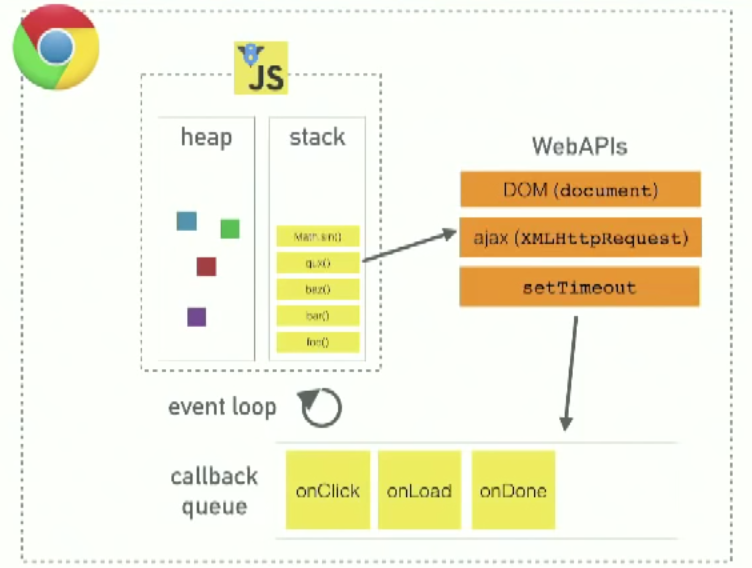
\includegraphics[width=0.75\textwidth]{images/js_event_loop.png}
\end{figure}

\subsection{Asynchronous programming}

Rxjs is a popular, stream based implementation of the observer-pattern.

\begin{lstlisting}
export interface Observer<T> {
    onNext: (val: T) => void,
    onCompleted: () => void,
    onError: (e: Error) => void
}


const nullObserver: Observer<any> = {
    onNext: (val: any) => {},
    onCompleted: () => {},
    onError: (e: Error) => {}
}


/**
 * Subscriptions are just handles to observers,
 * so that they can be unsubscribed if need be.
 */
export interface Subscription {
    unsubscribe: () => void;
}


export class SimpleSubscription<T> implements Subscription {
    constructor(
        private observer: Observer<T>
    ) {}

    unsubscribe () {
        // unsupscription == overwrite original observer
        this.observer = nullObserver;
    }
}


/**
 * 
 */
export class Observable<T> {

    constructor(
        private _subscribe: (observer: Observer<T>) => Subscription
    ) {}


    subscribe(downstreamObserver: Observer<T>): Subscription {
        return this._subscribe(downstreamObserver);
    }


    /**
     * List of static creational methods.
     * They each return new observables. 
     * Note that those new observables do not execute the _subscribe mehtod yet.
     * that method is only executed when subscribe is executed. 
     */

    static of<X>(args: X[]): Observable<X> {
        return new Observable<X>((downstreamObserver: Observer<X>) => {
            console.log(`executing subscription-body (returned from 'of' method)`)

            args.forEach(val => downstreamObserver.onNext(val));
            downstreamObserver.onCompleted();

            return new SimpleSubscription(downstreamObserver);
        })
    }


    static fromEvent(source: Element, event: string): Observable<Event> {
        return new Observable<Event>((downstreamObserver: Observer<Event>) => {
            console.log(`executing subscription-body (returned from 'fromEvent' method)`)

            const callback = (e: Event) => downstreamObserver.onNext(e);
            source.addEventListener(event, callback);
            return {
                unsubscribe: () => source.removeEventListener(event, callback)
            }
        });
    }

    /**
     * list of non-static creational mehtods.
     * They each return new observables.
     * Note that the subscribe methods are not called yet with this method.
     */

    map<Y>(mapFunc: (v: T) => Y): Observable<Y> {
        return new Observable<Y>((downstreamObserver: Observer<Y>) => {
            console.log(`executing subscription-body (returned from 'map' method)`)

            const mappingObserver: Observer<T> = {
                onNext: (val: T) => {
                    const y: Y = mapFunc(val);
                    downstreamObserver.onNext(y);
                },
                onCompleted: () => downstreamObserver.onCompleted(),
                onError: (e: Error) => downstreamObserver.onError(e)
            };

            return this.subscribe(mappingObserver);
        });
    }


    filter(filterFunc: (v: T) => boolean): Observable<T> {
        return new Observable<T>((downstreamObserver: Observer<T>) => {
            console.log(`executing subscription-body (returned from 'filter' method)`)

            const filteringObserver: Observer<T> = {
                onNext: (val: T) => {
                    if (filterFunc(val)) {
                        downstreamObserver.onNext(val);
                    }
                },
                onCompleted: () => downstreamObserver.onCompleted(),
                onError: (e: Error) => downstreamObserver.onError(e)
            };

            return this.subscribe(filteringObserver);
        });
    }


    take(nr: number): Observable<T> {
        return new Observable<T>((downstreamObserver: Observer<T>) => {
            console.log(`executing subscription-body (returned from 'take' method)`)

            let i = 0;
            const takingObserver: Observer<T> = {
                onNext: (val: T) => {
                    if (i < nr) {
                        downstreamObserver.onNext(val);
                        i += 1;
                    } else {
                        downstreamObserver.onCompleted();
                    }
                },
                onCompleted: () => downstreamObserver.onCompleted(),
                onError: (e: Error) => downstreamObserver.onError(e)
            };

            return this.subscribe(takingObserver);
        })
    }

}

const list$ = Observable.of([1, 2, 3, 4, 5, 6, 7, 8]);

const list2$ = list$.map((v) => v+1);

const list3$ = list2$.filter((v) => v % 2 === 1);

const list4$ = list3$.take(3);

list4$.subscribe({
  onNext: (val: number) => console.log(val),
  onCompleted: () => {}, 
  onError: () => {}
});
\end{lstlisting}

Zones allow you to wrap multpile, potentially asynchronous callframes in one common environment.

\begin{lstlisting}
interface ZoneSpec {
    name: string;
    props?: object;
    onFork?;
    onIntercept?;
    onInvoke?;
    onScheduleTask?;
    onInvokeTask?;
    onCancelTask?;
    onHasTask?;
}
    
class Zone {
    private static _current: Zone = new Zone(null, {name: 'Base'});
    private _parent: Zone;
    private zoneSpec: ZoneSpec;
    
    constructor(parent: Zone, zoneSpec: ZoneSpec) {
        this._parent = parent;
        this.zoneSpec = zoneSpec;
    }
    
    static get current() {
        return Zone._current;
    }
    
    get name() {
        return this.zoneSpec.name;
    }
    
    get parent() {
        return this._parent;
    }
    
    get(key: string) {
        return this.zoneSpec.props ? this.zoneSpec.props[key] : null;
    }
    
    fork(newZoneSpec: ZoneSpec) {
        for (const key in this.zoneSpec) {
        if (key != 'name') {
            if (!newZoneSpec[key]) {
            newZoneSpec[key] = this.zoneSpec[key];
            }
        }
        }
        return new Zone(Zone.current, newZoneSpec);
    }
    
    run(callback) {
        Zone._current = this;
        callback();
        Zone._current = this.parent;
    }
    
}


const _setTimeout = (callback, time) => {
const zoneOnCreateTime = Zone.current;
const wrappedCallback = () => {
    zoneOnCreateTime.run(callback);
};
setTimeout(wrappedCallback, time);
}


const zoneBC = Zone.current.fork({
name: 'BC',
props: {
    message: "Hi! You can only see me inside BC!"
}
});


function c() {
console.log("executing c in zone ", Zone.current.name);
console.log("Here's the message data: ", Zone.current.get('message'));
}

function b() {
console.log("executing b in zone ", Zone.current.name);
console.log("Here's the message data: ", Zone.current.get('message'));
_setTimeout(c, 2000);
// c();
}

function a() {
console.log("executing a in zone ", Zone.current.name);
console.log("Here's the message data: ", Zone.current.get('message'));
zoneBC.run(b);
}

a();
console.log("this is root, running in zone ", Zone.current.name);
\end{lstlisting}

\subsection{Module system}


\begin{table}[ht]
    \begin{tabularx}{1.2\textwidth}{XXXXXX}
        & CommonJs                                                            & NodeJs                                                                   & AMD                                                                              & UMD                                                           & ES2015 aka. ES6                                           \\
        used by         & formerly node                                                       & node                                                                     & requirejs                                                                        &                                                               &                                                           \\
        module-file     & \inlinecode{exports.area = (r) = PI * r * r;}                       & \inlinecode{module.exports = \{area: (r) = PI * r * r; \}}               & \inlinecode{define}                                                              & First tries AMD, then commonJs, then exports as global.       & \inlinecode{export const sqrt = Math.sqrt;}               \\
        user-file       & \inlinecode{const module = require('./module.js'); module.area(4);} & \inlinecode{const module = require('./module.js'); module.area(4);}      & \inlinecode{require, import, module}                                             &                                                               & \inlinecode{\{import \{ sqrt \} from 'module';\}}         \\
        loads modules   & synchronously                                                       & synchronously                                                            & asynchronously                                                                   &                                                               &                                                           \\
        implementations & webpack, browserify                                                 & node, webpack, browserify                                                & requirejs                                                                        &                                                               & webpack, babel                                            \\
        Notes           & Used to be a candidate for node, but now abandoned.                 &                                                                          & Does not work well with node (there is amdefine to help, but not ideal, either). &                                                               & Official JS standard, but so far not implemented in any browser or nodejs.
    \end{tabularx}
\end{table}

    

\subsubsection{Building with webpack}
My builder of choice is webpack. Basically, webpack makes ES6-import and -export work. There is some nice documentation \href{https://what-problem-does-it-solve.com/webpack/index.html}{here}.

paragraph{General concepts}: Some concepts and nomenclature.

\begin{itemize}
    \item Loaders vs Plugins: loaders work on the individual file-level, plugins work at the bundle- or chunk-level.
    \item compiling: compiling means transforming (eg.) ts-code to some (older version of) js.
    \item bundling: bundling takes compiled code and uses the import statements to create one large file.
\end{itemize}

\paragraph{Module-resolution}: Webpack can work with most module-types that javascript has to offer.

\begin{itemize}
    \item Javascript: webpack works fine with commonJs, nodeJs, and AMD, but will sometimes have problems with UMD.
        \begin{itemize}
            \item if a package.json has a \emph{module} entry, this field indicates that there is a ES6 version of the code. This will be loaded then.
            \item if it has a \emph{main} entry, that one leads to the entry-file of a (usually UMD) module.
            \item otherwise, you cannot import a whole module, but must load by filename.
        \end{itemize}
    \item Typescript: \inlinecode{ import { b } from "moduleB"; }. If in tsconfig the property \inlinecode{compilerOptions.module} is not \inlinecode{'AMD' | 'System' | 'ES2015'}, then a variation of the node-resolution is used:
        \begin{itemize}
            \item \inlinecode{'/node_modules/moduleB.ts'}
            \item \inlinecode{'/node_modules/moduleB.tsx'}
            \item \inlinecode{'/node_modules/moduleB.d.ts'}
            \item \inlinecode{'/node_modules/moduleB/package.json'}  (if it specifies a "types" property)
            \item \inlinecode{'/node_modules/@types/moduleB.d.ts'}
            \item \inlinecode{'/node_modules/moduleB/index.ts'}
            \item \inlinecode{'/node_modules/moduleB/index.tsx'}
            \item \inlinecode{'/node_modules/moduleB/index.d.ts'}
        \end{itemize}
    \item A note on Typescript's \inlinecode{import} and \inlinecode{require} statements: With TypeScript, \inlinecode{import} can be used if there is a declaration file for the module. If there isn't a declaration file, the TypeScript compiler doesn't know if the module exists, so you need to use \inlinecode{require} instead which lacks the compilation checking.
    \item Other languages: how to resolve other languages (ts, coffee, sass, shader, ...) is left over to loaders.
\end{itemize}

\paragraph{Shimming}: Webpack only loads a module when it sees it required at some point. This makes for smaller bundles, of course, but here is one problem this can cause. Say you have a dependency to jQuery and bootstrap. JQuery exposes \inlinecode{window.\$} as a global object. Bootstrap requires there to be a global \inlinecode{window.\$} object. However, since bootstrap just assumes that \inlinecode{window.\$} is there without ever calling \inlinecode{import}, webpack won't resolve the dependency and never include jQuery in the package. To avoid such problems, there is something called \emph{shimming}. 

\begin{lstlisting}
plugins: [
    new CopywebpackPlugin([ \{ from: path.resolve(__dirname, 'node_modules/cesium/Build/Cesium/Workers'), to: 'Workers' \} ]),
    new CopywebpackPlugin([ \{ from: path.resolve(__dirname, 'node_modules/cesium/Source/Assets'), to: 'Assets' \} ]),
    new CopywebpackPlugin([ \{ from: path.resolve(__dirname, 'node_modules/cesium/Source/Widgets'), to: 'Widgets' \} ]),
    new webpack.DefinePlugin(\{
        CESIUM_BASE_URL: JSON.stringify(''),
    \}),
    new webpack.ProvidePlugin(\{
        Cesium: 'cesium/Build/Cesium/Cesium'
    \})
],
\end{lstlisting}

The \inlinecode{ProviderPlugin} makes Cesium available to the global workspace. If you don't want this, you might want to instead use the \inlinecode{module.rules.imports-loader}.

\paragraph{Path-resolution}: When you ask to import a string that doesn't have a leading \inlinecode{./}, it tells Webpack: "Look for the file everywhere on my hard drive except the current directory". I'm not kidding. You can see the output desperately climbing up your directory hierarchy looking for a directory called \inlinecode{node_modules} in which it hopes to find index.js.
When you precede the module name with a \inlinecode{./}, it tells Webpack to look in the current directory for the file. So, the rule of thumb is: your code usually has a ./ and third-party libraries don't.

\paragraph{3rd party libs} d3 is a good example of a big library moving to the new ES6 module-syntax. d3 has many 3rd party libs that depend on and extend d3. As of D3 4.0, none of the D3 modules (formerly known as plugins) rely on a global d3 object. Each module is available either as a UMD bundle for use in Node or browsers, and as ES modules for use in bundlers and other modern JavaScript environments. Note that d3-plus hsa somehow still not managed to switch.

\paragraph{How webpack does it}
Webpack compiles this code:
\begin{lstlisting}
// helpers.ts
export function sayHi(name: string): string {
    return `Hi, ${name}!`;
}

// index.ts
import { sayHi } from "./helpers";
console.log(sayHi('Michael'));
\end{lstlisting}

to this code: 
\begin{lstlisting}
// self calling function
(function(modules) {
        // The module cache
        var installedModules = {};
    
        // The require function
        function __webpack_require__(moduleId) {
    
            // Check if module is in cache
            if(installedModules[moduleId]) {
                return installedModules[moduleId].exports;
            }
            // Create a new module (and put it into the cache)
            var module = installedModules[moduleId] = {
                i: moduleId,
                l: false,
                exports: {}
            };
    
            // Execute the module function
            modules[moduleId].call(module.exports, module, module.exports, __webpack_require__);
    
            // Flag the module as loaded
            module.l = true;
    
            // Return the exports of the module
            return module.exports;
        }
    
        // expose the modules object (__webpack_modules__)
        __webpack_require__.m = modules;
    
        // expose the module cache
        __webpack_require__.c = installedModules;
    
        // define getter function for harmony exports
        __webpack_require__.d = function(exports, name, getter) {
            if(!__webpack_require__.o(exports, name)) {
                Object.defineProperty(exports, name, { enumerable: true, get: getter });
            }
        };
    
        // define __esModule on exports
        __webpack_require__.r = function(exports) {
            if(typeof Symbol !== 'undefined' && Symbol.toStringTag) {
                Object.defineProperty(exports, Symbol.toStringTag, { value: 'Module' });
            }
            Object.defineProperty(exports, '__esModule', { value: true });
        };
    
        // create a fake namespace object
        // mode & 1: value is a module id, require it
        // mode & 2: merge all properties of value into the ns
        // mode & 4: return value when already ns object
        // mode & 8|1: behave like require
        __webpack_require__.t = function(value, mode) {
            if(mode & 1) value = __webpack_require__(value);
            if(mode & 8) return value;
            if((mode & 4) && typeof value === 'object' && value && value.__esModule) return value;
            var ns = Object.create(null);
            __webpack_require__.r(ns);
            Object.defineProperty(ns, 'default', { enumerable: true, value: value });
            if(mode & 2 && typeof value != 'string') for(var key in value) __webpack_require__.d(ns, key, function(key) { return value[key]; }.bind(null, key));
            return ns;
        };
    
        // getDefaultExport function for compatibility with non-harmony modules
        __webpack_require__.n = function(module) {
            var getter = module && module.__esModule ?
                function getDefault() { return module['default']; } :
                function getModuleExports() { return module; };
            __webpack_require__.d(getter, 'a', getter);
            return getter;
        };
    
        // Object.prototype.hasOwnProperty.call
        __webpack_require__.o = function(object, property) { return Object.prototype.hasOwnProperty.call(object, property); };
    
        // __webpack_public_path__
        __webpack_require__.p = "";
    
    
        // Load entry module and return exports
        return __webpack_require__(__webpack_require__.s = 0);
    })({
    
        // dependency
        "./src/dependency.ts": (function(module, __webpack_exports__, __webpack_require__) {
            function sayHi(name) {
                return "Hi, " + name + "!";
            }
            __webpack_require__.r(__webpack_exports__);
            __webpack_require__.d(__webpack_exports__, "sayHi", function() { return sayHi; })
        }),
    
        // script 
        "./src/index.ts": (function(module, __webpack_exports__, __webpack_require__) {
            __webpack_require__.r(__webpack_exports__);
            var _helpers__WEBPACK_IMPORTED_MODULE_0__ = __webpack_require__("./src/helpers.ts");
            console.log(Object(_helpers__WEBPACK_IMPORTED_MODULE_0__["sayHi"])('Michael'));
        })
});
\end{lstlisting}


\subsection{Promises, async-await and rxjs}
\inlinecode{async} - \inlinecode{await} lets you handle asynchronous code as if it was synchronous. 

\subsection{Webworkers: multithreading}


\subsection{WASM}
\begin{itemize}
    \item If wasm does not get a garbage-collector, 
        \begin{itemize}
            \item there will be no easy way for non-gc languages to run in wasm. They need to bring their own gc (or even runtime) with them (like c\# does now). 
            \item In that case, a situation like python + numy will probably evolve.
        \end{itemize}
    \item If wasm will not allow DOM-manipulation, 
        \begin{itemize}
            \item then there really is no point for non nummeric-focussed languages to be implemented in wasm.
            \item In that case, a situation like python + numy will probably evolve.
        \end{itemize}
    \item If, however, wasm will get a gc and allow DOM-manipulation, 
        \begin{itemize}
            \item Then python, ruby etc. will all develop angular-clones to run on the web. 
            \item However, given the large js-ecosystem, those will not kick in too mightily. 
        \end{itemize}
\end{itemize}


\section{CSS}

\subsection{Position}
\begin{itemize}
    \item \textbf{static}: the default
    \item \textbf{relative}: default + allows top, bottom, left and right
    \item \textbf{fixed}: relative to viewport
    \item \textbf{absolute}: relative to nearest positioned parent (positioned: anything but static)
    \item \textbf{sticky}: like fixed, but relative to container instead of viewport.
\end{itemize}

\subsection{Display}
Per default, divs are dispayed in blockstyle, while spans are displayed inlinestyle.
\begin{itemize}
    \item \textbf{block}
    \item \textbf{inline}
    \item \textbf{inline-block}: inline, but allows width, heigth, padding etc.
    \item \textbf{none}
    \item \textbf{table}
    \item \textbf{grid}
    \item \textbf{flex} see \ref{flexbox}
\end{itemize}

\subsubsection{Flexbox}\label{flexbox}


\section{Git}

\subsection{Lingo}
\begin{itemize}

    \item origin: default name for your remote repository
    
    \item head: \emph{your} last \emph{commit} on the current branch. Does not yet include non-commited changes. 
        \begin{itemize}
            \item When you switch branches with \inlinecode{git checkout}, the HEAD revision changes to point to the tip of the new
            branch.
            \item When you do a \inlinecode{git pull}, your working directory may contain new stuff, which your head is lagging behind. To see the difference between the working dir and your last commit, do \inlinecode{git diff HEAD}
        \end{itemize}
        
    \item index: The index is a single, large, binary file in baseOfRepo/.git/index, which lists all files in the current branch, their sha1 checksums, time stamps and the file name
    
\end{itemize}

\subsection{Branches}

\paragraph{Creating a new branch} Don't forget to also specify the branches name when you push:

\begin{lstlisting}
git branch schwebstoff_tabellen
git branch
git checkout schwebstoff_tabellen

# ... doing stuff ...

git push -u origin schwebstoff_tabellen
\end{lstlisting}

\paragraph{Checking out an existing branch} Just first clone the whole repo and then switch to the branch: 

\begin{lstlisting}
git clone http://hnd-jens.rz-sued.bayern.de:8181/applikation/includes.git
git branch -a // also shows remote branches
git fetch origin schwebstoff_tabellen
git checkout schwebstoff_tabellen
\end{lstlisting}


\paragraph{Merging a branch back into master} On the dev-branch, we first suck in all the changes that might have occured on the master while we were not looking. Once those changes have been properly integrated, we switch to the master and suck in the dev-branch.

\begin{lstlisting}
// Step 0: safety measure: first get all new stuff from the master into your dev branch
git merge master 

// Step 1: Go to master and insert all your dev stuff 
checkout master
git merge schwebstoff_tabellen

// Step 2: cleanup
git branch --merged master // see all branches that have already been merged
git branch -d shwebstoff_tabellen  // don't need this branch any more
git push origin --delete schwebstoff_tabellen // also remove on remote

// Step 3: push
git push -u origin master
\end{lstlisting}


\paragraph{Merging remote changes on master into local master} It can happen that somebody else has been messing with the master before you had a chance to commit your own changes. You will notice this by seeing your \inlinecode{git push} fail. In that case, try to first merge the remote changes into your local copy before pushing again. 
\begin{lstlisting}
git commit // first saving our latest changes
git fetch  // geting remote stuff in remote-tracking-branches. Doesn't change our files yet
git diff master origin/master // compares what you have in master vs. what happend to master remotely
git merge remotes/origin/master
\end{lstlisting}
This will try to merge the upstream changes into yours. If it fails, the conflicting file will contain annotations like these: 
\begin{lstlisting}
<<<<<<< HEAD
print("159 just edited this file")
=======
print("133 just edited this file")
>>>>>>> master
\end{lstlisting}
As you can guess, \inlinecode{<<<<<HEAD} is your code, \inlinecode{===} is a separator, and \inlinecode{>>>> master} is the end of the other guys code. 
Use a texteditor to resolve all conflicts. Eclipse actually has a graphical interpreter for the conflict-tags. Once the resolving is completed, a \inlinecode{git push} and \inlinecode{git commit} will complete the merge.
\begin{lstlisting}
git status // shows that there is still a conflict
git add .
git status // shows that conflict is resolved, but merging still in progress
git commit -m "phew! managed to resolve the conflict!"
git push origin master
\end{lstlisting}


\paragraph{Comparing branches} Diff can compare any commited branches: 
\begin{lstlisting}
// How is your branch different from the master?
git diff master..schwebstoff_tabellen
// What have you changed since your last commit?
git diff HEAD
\end{lstlisting}

\paragraph{Reverting and resetting} is best explained in this post: \inlinecode{https://stackoverflow.com/questions/4114095/how-to-revert-git-repository-to-a-previous-commit}. Basically, we have these options: 

\begin{itemize}
    \item \inlinecode{git revert <lastGoodCommitHash>..HEAD} will execute the inverse of all the operations and commit them as a new commit. This way, the old history stays intact.
    \item \inlinecode{git reset <lastGoodCommitHash>} will delete all the commits from \inlinecode{<firstBadCommitHash>..HEAD}. This way, you're rewriting history, which is really only good if you're working alone on a repo.
\end{itemize}



\subsection{Creating your own repository}
Basically, any git folder can be used as a repository. But you still need to do some work to expose that folder over the web. The easiest way to work is certainly over gitlab. For alternative means if you don't have a hoster, this site lists a few of the possibilities: \inlinecode{http://www.jedi.be/blog/2009/05/06/8-ways-to-share-your-git-repository/}.



\subsection{Storing credentials}
It is tedious to always have to type your name and password again. Here's how to avoid that: 
\begin{lstlisting}
git config [--global] user.name "Mona Lisa"
git config [--global] credential.helper "cache --timeout=3600"
\end{lstlisting}

\paragraph{Changing origin}
\begin{lstlisting}
git remote -v
git remote set-url origin https://github.com/USERNAME/REPOSITORY.git
\end{lstlisting}

%\section{Strategies}

\subsection{Dependencies versus microservices}

Dependencies can be included right in your sourcode. Microservices on the other hand are not included at all, but called remotely from your programm. 


\begin{table}[h]
\centering
\caption{Dependencies versus microservices}
\begin{tabular}{@{}lllll@{}}
\toprule
        & Dependencies                                             & Microservices                                                      &  &  \\ \midrule
Changes & You can include the exact needed version of a dependency & Your program needs to adapt immediately if the service API changes &  &  \\
        &                                                          &                                                                    &  &  \\
        &                                                          &                                                                    &  &  \\ \bottomrule
\end{tabular}
\end{table}




\subsection{Branching strategies}

\chapter{Applications}
\section{Where should we meet?}

$n$ people want to decide at who's house to meet up. Does it matter? Can the sum of the paths that each person needs to travel vary? In fact, it can! Imagine that $n-1$ of them live in the same town, while the last of them lives far away on the other side of the country. If they all meet in the town, only one person has to travel very far, whereas if they meet on the other side of the country, $n-1$ people need to travel a large distance.


The distance to travel can be represented by a weighted connection matrix. Consider this example:

$$
\begin{bmatrix}
    0 &  1 &  1 &  1 &  11 \\
    1 &  0 &  1 &  1 &  11 \\
    1 &  1 &  0 &  1 &  11 \\
    1 &  1 &  1 &  0 &  10 \\
    11 & 11 & 11 & 10 & 0 \\
\end{bmatrix}
$$

It is now trivial to see that we can find the optimal place to meet up as the column with the smallest sum - in this case this would be at the place of person $d$.

\section{Effective wind on a ship}
A ship can only take the force of the wind that is aligned with its own angle. To calculate the vector of the wind for the ship, we must project the actual wind-vector onto the ships direction-vector. 

\section{Making a touch-instrument}

\subsection{Music}

\subsubsection{Notes}
A single tone $x$ has only two atributes: frequency $f_x$ and amplitude $a_x$ a.k.a. pitch and loudness . The wave of a note is a function of these two: $w_x(t) = a_x \cdot \sin( f_x \cdot t)$

In practice, a note will stop being played at some time. Therefore, the real function for a note would be $w_x(t) \cdot s(t_1, t_2)$, where $s$ is a step function. In FFT, however, we mostly treat a note as if it were a real periodic function - that is, never ending. We'll see details of this later. 

By the way: The same note played on a piano still sounds different from a violin because physical instruments never play one pure note. Instead, depending on the material, different overtones are played along with the basenote. 

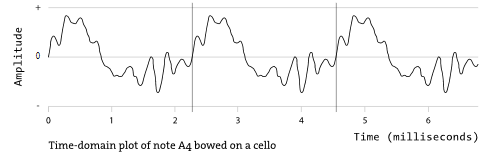
\includegraphics[width=10cm]{tdp.png}


\subsubsection{Harmony}
Instruments nowadays are tuned based on $a$, at 440 Hz. An octave higher would be $a'$ at 880 Hz. There are twelve steps from $a$ to $a'$, but their frequencies are not linearly, but exponentially spaced: 

\begin{itemize}
    \item linear: $f_x = \frac{12 + x}{12} f_a$
    \item exponential: $f_x = 2^{\frac{x}{12}} f_a$
\end{itemize}

Some combinations sound nice together:

\begin{itemize}
    \item Dur: {0,4,7}; $w(t) = w_a(t) + w_{cis}(t) + w_e(t)$
    \item Dur-Sept: {0,4,7,11}; $w(t) = w_a(t) + w_{cis}(t) + w_e(t) + w_{gis}(t)$
    \item Moll: {0,3,7}; $w(t) = w_a(t) + w_{c}(t) + w_e(t)$
    \item Moll-Sept: {}
\end{itemize}

They do sound nice together when the wave of their sum does display a nice pattern of peaks - that is, when the sum, too, displays a repeating pattern.

\subsubsection{Songs}

Several tones can be played together, thus adding up their waves: $w(t) = \sum_x w_x(t)$ Also, with every beat, new notes may be played. Thus for every beat a new analysis is required. 

\subsection{Deconstructing w(t) into fx and ax: the FFT}

The sound we hear in a song is really just a timeseries. Its values are the sum of the current amplitudes of all notes, i.o.w. it's just one single, complicated wave $w(t)$. The FFT takes that wave, chops it into windows of, say, a second, and tries to deconstruct the signal in each window into the original, simple waves $w_x(t)$ of the single notes $x$. 

So there are four steps to displaying a songs tones:

\begin{enumerate}
    \item Chop the signal into parts using the window-function (usually just a step-function). The window-function's length should be equal to the length of one beat.
    \item Take the first part and artificially elongate it by duplicating it over and over, thus creating a periodic signal.
    \item Do the FFT: represent this periodic signal as a sum of sines of different frequencies and amplitudes.
    \item Plot this.
    \item Repeat from step two with the next part of the choped-up signal.
\end{enumerate}

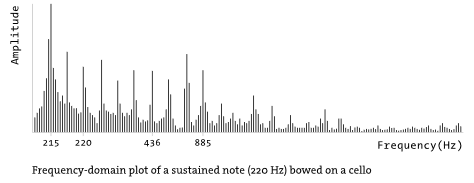
\includegraphics[width=10cm]{fdp.png}

\section{Drawing a room onto a cylinder}


The idea here is to imagine a scene taking place in a room. That scene is projected and drawn onto a paper cylinder. This way, a visitor can step inside the cylinder and see the scene around him as if he was actually there. 

This requires two projections to happen to the objects in the scene. Fist we need to project them onto the cylinder. Second we need to roll out the cylinder so that we can actually print the scene on it with a printer or by hand. 

\subsection{Projecting a line in space onto a cylinder}

We want to project the line from $\vec{a} = (10, 10, 1)$ to $\vec{b} = (0, 10, 1)$ onto a cylinder of radius $r=1$. We assume that the visitors eyes will be at the coordinates $\vec{c} = (0, 0, 1.6)$.

\subsubsection{Projecting a point onto the cylinder}

\subsubsection{Projecting a plane onto the cylinder}

So we found out where the two edge points of the line should go onto the cylinder. But what would the line connecting them look like? What we need here is the intersection of the cylinder with the plane  defined by the points $\vec{a}, \vec{b}, \vec{c}$. That plane is expressed as $P = \{ \vec{x} | 0.07y + z = 1.7 \}$.

To find the line we need an expression for $P \intersection C$, that is, a sollution to the system: 

$$ 0.07 y + z = 1.7 $$
$$ x^2 + y^2 = 1 $$

We can factor out $y$, leaving us with $x^2 + (\frac{1.7 - z}{0.07})^2 = 1$

\subsection{Rolling out the cylinder}

We cut the cylinder open along the $z$ axis. That means that for every $z$, we will apply a mapping $(x,y,z) \to (\theta, z)$. One particular mapping really stands out for that purpose - the polar representation of coordinates. Remember that 

$$ cos \theta = \frac{\vec{v}\vec{u}}{|\vec{v}||\vec{u}|}$$

This means that we can achieve our mapping by using $(x,y,z) \to (cos^{-1}x, z)$.


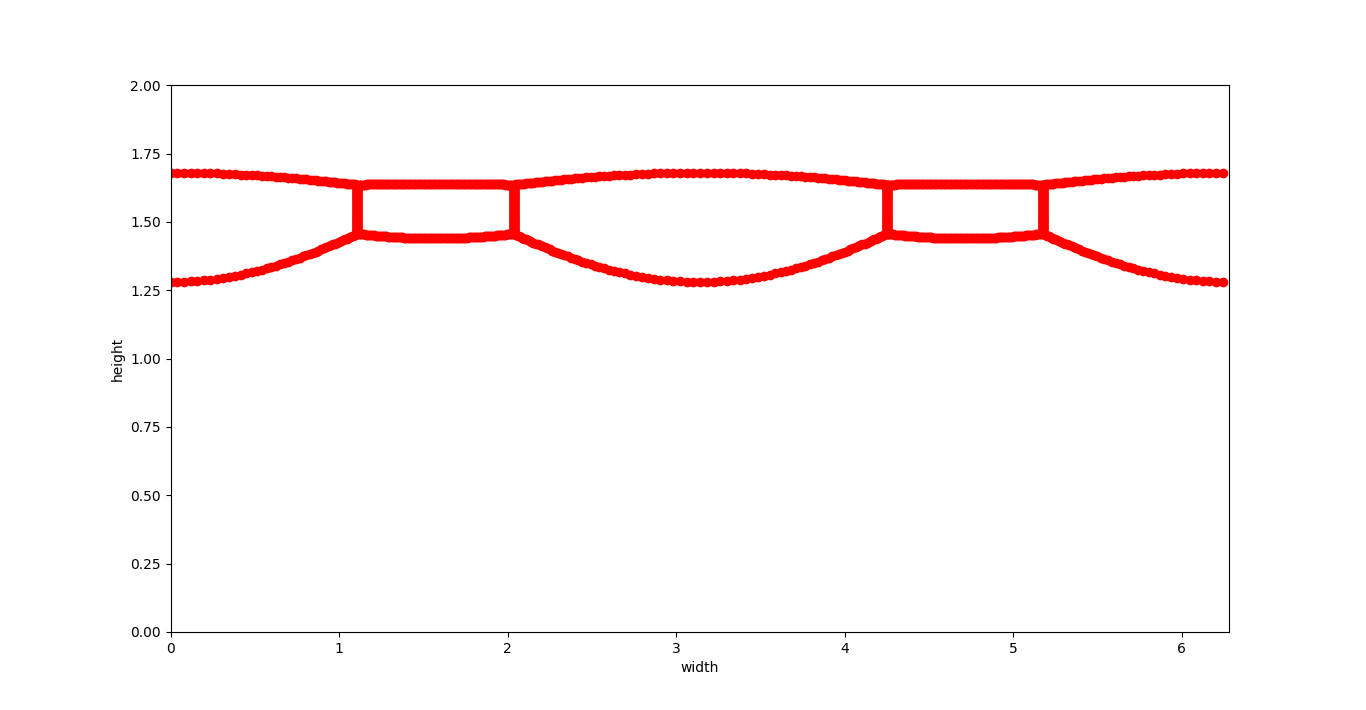
\includegraphics[width=0.8\textwidth]{images/room.png}

\begin{lstlisting}[language=python]
import matplotlib.pyplot as plt
from math import sqrt, pi, acos, atan


def distance(point1, point2):
    return sqrt((point2[0] - point1[0])**2 +
                (point2[1] - point1[1])**2 +
                (point2[2] - point1[2])**2)


def makeLine(point1, point2, num=100):
    line = []
    deltax = float(point2[0] - point1[0])/num
    deltay = float(point2[1] - point1[1])/num
    deltaz = float(point2[2] - point1[2])/num
    for i in range(num):
        x = point1[0] + i*deltax
        y = point1[1] + i*deltay
        z = point1[2] + i*deltaz
        line.append([x, y, z])
    return line


def intersection(point, head, cylinder):
    rc = cylinder.radius
    xp = point[0]
    yp = point[1]
    xh = head[0]
    yh = head[1]
    alpha1 = (xh**2 - xh*xp + yh**2 - yh*yp - sqrt(rc**2*xh**2 - 2*rc**2*xh*xp + rc**2*xp**2 + rc**2*yh**2 - 2*rc**2*yh*yp + rc**2*yp**2 - xh**2*yp**2 + 2*xh*xp*yh*yp - xp**2*yh**2)) / (xh**2 - 2*xh*xp + xp**2 + yh**2 - 2*yh*yp + yp**2)
    alpha2 = (xh**2 - xh*xp + yh**2 - yh*yp + sqrt(rc**2*xh**2 - 2*rc**2*xh*xp + rc**2*xp**2 + rc**2*yh**2 - 2*rc**2*yh*yp + rc**2*yp**2 - xh**2*yp**2 + 2*xh*xp*yh*yp - xp**2*yh**2)) / (xh**2 - 2*xh*xp + xp**2 + yh**2 - 2*yh*yp + yp**2)
    ints1 = [0, 0, 0]
    ints1[0] = head[0] + alpha1*(point[0] - head[0])
    ints1[1] = head[1] + alpha1*(point[1] - head[1])
    ints1[2] = head[2] + alpha1*(point[2] - head[2])
    dist1 = distance(ints1, head)
    ints2 = [0, 0, 0]
    ints2[0] = head[0] + alpha2*(point[0] - head[0])
    ints2[1] = head[1] + alpha2*(point[1] - head[1])
    ints2[2] = head[2] + alpha2*(point[2] - head[2])
    dist2 = distance(ints2, head)
    if dist2 > dist1:
        return ints1
    else:
        return ints2


def toPolar(point):
    pointPolar = [0, 0, 0]
    radius = sqrt(point[0]**2 + point[1]**2)
    #theta = acos(point[0]/radius) * 360.0 / (2*pi)
    theta = atan(point[1]/(point[0] + 0.000001)) * 360.0 / (2*pi)
    if point[0] >= 0 and point[1] >= 0:  # first quad
        theta = theta
    elif point[0] < 0 and point[1] >= 0:  # second quad
        theta = theta + 180
    elif point[0] < 0 and point[1] < 0:  # third quad
        theta = theta + 180
    else:
        theta = theta + 360
    pointPolar[0] = theta
    pointPolar[1] = radius
    pointPolar[2] = point[2]
    return pointPolar


def rollout(point, cylinder):
    pointPolar = toPolar(point)
    newpoint = [0, 0]
    newpoint[0] = 2*pi*cylinder.radius*pointPolar[0]/360
    newpoint[1] = point[2]
    return newpoint


class Cylinder:
    def __init__(self, radius):
        self.radius = radius


cylinder = Cylinder(1)
circumference = 2*pi*cylinder.radius
head = [0, 0, 1.6]
n = 100

# floor
line1 = makeLine([5, 10, 0], [-5, 10, 0], n)
line2 = makeLine([-5, 10, 0], [-5, -10, 0], n)
line3 = makeLine([-5, -10, 0], [5, -10, 0], n)
line4 = makeLine([5, -10, 0], [5, 10, 0], n)

# walls
line5 = makeLine([5, 10, 0], [5, 10, 2], n)
line6 = makeLine([-5, 10, 0], [-5, 10, 2], n)
line7 = makeLine([-5, -10, 0], [-5, -10, 2], n)
line8 = makeLine([5, -10, 0], [5, -10, 2], n)

# ceiling
line9 = makeLine([5, 10, 2], [-5, 10, 2], n)
line10 = makeLine([-5, 10, 2], [-5, -10, 2], n)
line11 = makeLine([-5, -10, 2], [5, -10, 2], n)
line12 = makeLine([5, -10, 2], [5, 10, 2], n)

line = line1 + line2 + line3 + line4 + line5 + line6 + line7 + line8 + line9 + line10 + line11 + line12


out = []
for i in range(len(line)):
    point = line[i]
    ints = intersection(point, head, cylinder)
    projp = rollout(ints, cylinder)
    out.append(projp)
    pointPolar = toPolar(ints)
    #print "mapping [{},{},{}] via ints [{},{},{}] and via polar [{},{},{}] to flat [{},{}]".format(point[0], point[1], point[2], ints[0], ints[1], ints[2], pointPolar[0], pointPolar[1], pointPolar[2], projp[0], projp[1])


xflat = []
yflat = []
for i in range(len(line)):
    xflat.append(out[i][0])
    yflat.append(out[i][1])


plt.plot(xflat, yflat, 'ro')
plt.xlabel('width')
plt.ylabel('height')
plt.axis([0, circumference, 0, 2])
plt.show()
\end{lstlisting}

\section{Playing with projections and transformations}

I like to start with a simple basefunction, and then distort it.

Nice basefunctions:
\begin{itemize}
    \item simple geometric
    \item recursive
\end{itemize}

Nice distortions: 
\begin{itemize}
    \item sinusoidal (Fourier: add overtones)
    \item imaginary (Laplace: add more dimensions)
    \item stepfunction (Mandelbrot: cut off some of them)
    \item flat onto spherical (Mapprojection)
    \item circle rolled around circle (Spirograph)
    \item Copy and rotate
    \item shadows
\end{itemize}

Finally, we can refine the result. 
\begin{itemize}
    \item change paras over time
    \item heatmap
    \item path
\end{itemize}

We will try an example now. Take a simple geometric shape. Create it's fourier representation. Add some overtones to it. Convert it back into geometric space. What do you get?

There are basically two ways we can achive this. The first is using ordinary (that is, one-dimenstional) Fourier and parametrised shapes: 
\begin{itemize}
    \item a1: Take some parameterised Shape in $\reals^3$: $S(f(t))$
    \item a2: Extract $f(t)$
    \item a3: Express $f(t)$ in its Fourier representation: $f(t) = \sum \alpha_i b_i$, where $b_i$ is one-dimensional
    \item a4: add some overtones to obtain $f'(t)$
    \item a5: Obtain $S'$ as $S(f'(t))$ 
\end{itemize}

The second approach seems simpler, but requires tree dimensional Fourier: 
\begin{itemize}
    \item b1 (= a2): Take a shape $S(\vec{v})$
    \item b2 (= a3): $S(\vec{v}) = \sum \alpha_i \vec{b}_i$
    \item b3 (= a4, a5): Obtain $S'$ by adding overtones to $S$
\end{itemize}






\section{Fourier on sound and geometric objects}

\subsection{Basics: Fourier in one dimension}

\subsubsection{Representing a function under a Fourier base}

 The Fourier functions $\{sin(nt), cos(nt) | n \in \naturals \}$ form an orthogonal base for all functions in the space of square-integrable functions that are periodic between $-\pi$ and $\pi$. Lets first get some familiarity with Fourier analysis.

At first we'll try to express a simple function in a fourier base: 
$$ f(t) = sin(t) = \alpha_0 + \sum_n^\infty \alpha_n cos(n t)  + \sum_n^\infty \beta_n sin(n t)$$

It's comparatively easy to calculate the coefficients of this series\footnote{The term $\frac{1}{\pi}$ is not strictly neccessary for an orthogonal base, but it is very convenient, since it makes our base ortho\emph{normal}.}: 

$$ \alpha_0 = \frac{1}{\pi} \int_{-\pi}^\pi sin(t) \diff{t} = 0$$
$$ \alpha_1 = \frac{1}{\pi} \int_{-\pi}^\pi sin(t) cos(t) \diff{t} = 0$$
$$ \alpha_2 = .. = 0 $$
$$ \alpha_3 = ... = 0 $$

$$ \beta_1 = \frac{1}{\pi} \int_{-\pi}^\pi sin(t) sin(t) \diff{t} = 1 $$
$$ \beta_2 = \frac{1}{\pi} \int_{-\pi}^\pi sin(t) sin(2t) \diff{t} = 0 $$
$$ \beta_3 = ... = 0 $$ 

In other words: the only amplitude different from $0$ is $\beta_1 = 1$

We'll be using python for our Fourier-analysis, where it is more common to work with the exponential/imaginary representation of the Fourier functions. This representation is based on Eulers formula: 

$$ e^{it} = \cos(t) + i\sin(t)$$

Using this equation we can rewrite the Fourier base as $\{e^{int} | n \in \naturals \}$.
 Using this base we get as the only nonzero coefficient: 
 $$ \gamma_1 = \frac{1}{\pi} \int_{-\pi}^\pi sin(t) e^{it} \diff{t} = i $$

Having imaginary amplitudes may be intimidating at first, but really it's very simple. The real part of such an amplitude equals the amplitude of the equivalent $\cos$ term, whereas the imaginary part equals the amplitude of the $\sin$ term. 

\subsubsection{Bringing in arbitrary intervals}

In the previous section, when we wrote the index $n$, we meant that the function would repeat itself $n$ times within the interval $[-\pi, \pi]$ - it has a frequency of $f_n = \frac{n}{2\pi}$.

However, in reality we will deal with functions that are periodic over an unspecified interval $[-T,T]$ \footnote{In \emph{real} reality, we will not deal with periodic functions at all. But more on that later}. To acomodate this, we can expand our notion of Fourier basis to the space of all square integrable functions that are periodic between $[-T, T]$. Our base now consists of $\{sin(\frac{2 \pi n}{T} t), cos(\frac{2 \pi n}{T} t) | n \in \naturals \}$ or $\{ e^{i \frac{2 \pi n}{T} t} | n \in \naturals \}$.

Lets consider the function $f(t) = \sin(\frac{2\pi}{T}t)$. Just like before, it's easy to calculate this functions Fourier coefficients, and just like before, only one of them is nonzero: 

$$ \gamma_1 = \frac{1}{T} \int_{-T}^T \sin(\frac{2\pi}{T} t) e^{i \frac{2 \pi}{T} t} \diff{t} = i$$

The frequency that goes associated with the index $n=1$ is $f_n = \frac{n}{T} = 0.1$. 

\subsubsection{Implementation and verification in python}

It's time to get our hands dirty and learn about python's implementation of Fourier transforms. We'll try to use pythons \inlinecode{fft} library to recreate the previous section: 

\begin{lstlisting}
import numpy as np
import matplotlib.pyplot as plt

delta = 0.01
T = 10
t = np.arange(-T, T, delta)
data = np.sin(2 * np.pi * t / T)
amps = np.fft.fft(data)
frqs = np.fft.fftfreq(data.size, delta)

f, (ax1, ax2) = plt.subplots(1, 2)
ax1.plot(frqs, np.real(amps))
ax2.plot(frqs, np.imag(amps))
plt.show()
\end{lstlisting}

As expected, the plot shows a high amplitude at the frequency 0.1. Not quite as expected is the other peak at frequency -0.1. What's up with that? In fact, there are a few phenomena that warrant further explanation: 

\begin{itemize}
    \item Amplitudes are not really 0 where they should be, they only are very close to 0. This is merely an artifact of numerical computation that we won't bother with any further. 
    \item The amplitudes are not normalized to $T$. This, too, should not pose any difficulties for us, as we will not be using the concrete values of the amplitudes in this project. 
    \item How does fft chose which frequencies to consider? Here, for some reason, it's between -50 and 50.
    \item Why are there positive and negative frequencies?
    \item For now, we have chosen \inlinecode{t} to cover the interval $[-T, T]$ perfectly. But what if we have \inlinecode{t} too long or too short? Surprisingly, this doesn't seem to change the estimated frequencies very much. 
\end{itemize}


\subsubsection{Our first frequency domain operations: adding overtones}

We went trough all the trouble of representing $f(t)$ over a Fourier base for a reason: there are operations that are natural in the frequency domain that don't exactly come easily in time domain. One of those operations would be adding overtones. 


\begin{lstlisting}[language=python]
import numpy as np
import matplotlib.pyplot as plt
import simpleaudio as sa


sampleRate = 44100


def addXHalfTonesTo(basefreq, steps):
    return basefreq * (2 ** (steps / 12.0))


def play(data, sampleRate):
    dataNrm = data * 32767 / np.max( np.abs( data ))
    data16 = dataNrm.astype(np.int16)
    return sa.play_buffer(data16, 1, 2, sampleRate)



# creating the data
delta = 1.0 / sampleRate
T = 1
t = np.arange(0, T, delta)
data = np.sin( t * 440 * 2 * np.pi )
#play(data, sampleRate)


# transform to frequency domain
amps = np.fft.fft(data)
frqs = np.fft.fftfreq(data.size, delta)

# filter out the less important frqs
# add chord on top of basetone
thrsh = 0.1 * np.max(np.abs(amps))
ampsNew = np.zeros(np.shape(amps), dtype=np.complex128)
for i, a in enumerate(amps):
    if np.abs(a) > thrsh:
        f1 = frqs[i]
        f2 = np.round(addXHalfTonesTo(f1, 4))
        f3 = np.round(addXHalfTonesTo(f1, 7))
        i2 = np.where(frqs == f2)[0]
        i3 = np.where(frqs == f3)[0]
        ampsNew[i] += a
        ampsNew[i2] += a
        ampsNew[i3] += a

# convert back to timedomain
dataNew = np.fft.ifft(ampsNew)
play(dataNew, sampleRate)


# plot
f, ((ax1, ax2), (ax3, ax4)) = plt.subplots(2, 2)
ax1.plot(t, data)
ax2.plot(frqs, np.abs(amps))
ax3.plot(t, dataNew)
ax4.plot(frqs, np.abs(ampsNew))
plt.show()
\end{lstlisting}


\subsubsection{Windowing}
Now, in reality we will not be dealing with a allways constant sinewave. A piece of music is composed of different tones at different times. If we don't account for that, we get something like this: 

\begin{lstlisting}[language=python]
import numpy as np
import matplotlib.pyplot as plt
import simpleaudio as sa


sampleRate = 44100


def addXHalfTonesTo(basefreq, steps):
    return basefreq * (2 ** (steps / 12.0))


def play(data, sampleRate):
    dataNrm = data * 32767 / np.max( np.abs( data ))
    data16 = dataNrm.astype(np.int16)
    return sa.play_buffer(data16, 1, 2, sampleRate)



# creating the data
delta = 1.0 / sampleRate
T = 1
t = np.arange(0, T, delta)
fa = 440
fc = addXHalfTonesTo(fa, 4)
fd = addXHalfTonesTo(fc, 3)
a = np.sin( t * fa * 2 * np.pi )
c = np.sin( t * fc * 2 * np.pi )
d = np.sin( t * fd * 2 * np.pi )
t = np.concatenate((t, t, t, t))
data = np.concatenate((a, c, d, c))
#play(data, sampleRate)


# transform to frequency domain
amps = np.fft.fft(data)
frqs = np.fft.fftfreq(data.size, delta)

# filter out the less important frqs
# add chord on top of basetone
thrsh = 0.1 * np.max(np.abs(amps))
ampsNew = np.zeros(np.shape(amps), dtype=np.complex128)
for i, a in enumerate(amps):
    if np.abs(a) > thrsh:
        f1 = frqs[i]
        f2 = np.round(addXHalfTonesTo(f1, 4))
        f3 = np.round(addXHalfTonesTo(f1, 7))
        i2 = np.where(frqs == f2)[0]
        i3 = np.where(frqs == f3)[0]
        ampsNew[i] += a
        ampsNew[i2] += a
        ampsNew[i3] += a

# convert back to timedomain
dataNew = np.fft.ifft(ampsNew)
play(dataNew, sampleRate)


# plot
f, ((ax1, ax2), (ax3, ax4)) = plt.subplots(2, 2)
ax1.plot(t, data)
ax2.plot(frqs, np.abs(amps))
ax3.plot(t, dataNew)
ax4.plot(frqs, np.abs(ampsNew))
plt.show()

\end{lstlisting}


Thats why we use windowing. Windowing is the process of cutting an incomming signal in small chunks, for wich we create an individual Fourier analysis. This way, at tone c, we don't have to drag along tone a any more; a has long been forgotten by the analysis. 



\begin{lstlisting}[language=python]
import numpy as np
import matplotlib.pyplot as plt
import simpleaudio as sa


sampleRate = 44100


def first(data, cond):
    for i, d in enumerate(data):
        if cond(d):
            return i, d


def addXHalfTonesTo(basefreq, steps):
    return basefreq * (2 ** (steps / 12.0))


def overtone(steps, frqs, amps):
    ampsNew = np.zeros(np.shape(amps), dtype=np.complex128)
    for i, a in enumerate(amps):
        if np.abs(a) > 0: 
            f1 = frqs[i]
            f2 = np.round(addXHalfTonesTo(f1, steps))
            i2 = np.where(frqs == f2)
            #ampsNew[i] += a
            ampsNew[i2] += a
    return ampsNew
            

def play(data, sampleRate):
    dataNrm = data * 32767 / np.max( np.abs( data ))
    data16 = dataNrm.astype(np.int16)
    po = sa.play_buffer(data16, 1, 2, sampleRate)
    po.wait_done()
    return po


def filterLower(amps, perc):
    thrsh = perc * np.max( np.abs( amps ))
    ampsNew = np.zeros(np.shape(amps), dtype=np.complex128)
    for i, a in enumerate(amps):
        if np.abs(a) > thrsh: 
            ampsNew[i] = a
    return ampsNew


def distort(frqs, amps):
    ampsFiltered = filterLower(amps, 0.5)
    terz = overtone(4,frqs, ampsFiltered)
    quint = overtone(7, frqs, ampsFiltered)
    return ampsFiltered + terz + quint


def autotune(frqs, amps):
    ampsFiltered = filterLower(amps, 0.9999)
    ampsTuned = np.zeros( np.shape( ampsFiltered), dtype=np.complex128 )
    halfToneFreqs = [addXHalfTonesTo(220, x) for x in range(23)]
    for i, a in enumerate(ampsFiltered):
        if np.abs(a) > 0: 
            f = frqs[i]
            if f > 0:
                ihh, fhh = first(halfToneFreqs, lambda fc: fc >= f)
                fhl = halfToneFreqs[ihh-1]
                disth = np.abs(fhh - f)
                distl = np.abs(fhl - f)
                fh = fhl if distl < disth else fhh
                inew, fnew = first(frqs, lambda fc: fc >= fh)
                ampsTuned[inew] = a
    return ampsTuned
        

def chunks(data, length):
    C = int( np.ceil( len(data) / length ))
    chunks = []
    start = 0
    end = length
    for c in range(C):
        chunks.append(data[start:end])
        start += length
        end += length
    return chunks


delta = 1.0 / sampleRate
t = np.arange(0, 2, delta)
freq = lambda t: 220 + 220 * t / 2
data = np.sin(t * freq(t) * 2 * np.pi)

origAmps = []
tunedAmps = []
tunedChunks = []
chunksize = int(data.size / 4)
for chunk in chunks(data, chunksize):
    frqs = np.fft.fftfreq(chunk.size, delta)
    amps = np.fft.fft(chunk)
    ampsNew = autotune(frqs, amps)
    dataNew = np.fft.ifft(ampsNew)
    origAmps.append(amps)
    tunedAmps.append(ampsNew)
    tunedChunks.append(dataNew)


dataNew = np.concatenate(tunedChunks)
play(data, sampleRate)
play(dataNew, sampleRate)


start = 0
stop = 700
f, axes = plt.subplots(4)
for i in range(4):
    axes[i].plot(frqs[start:stop], np.abs(origAmps[i][start:stop]))
    axes[i].plot(frqs[start:stop], np.abs(tunedAmps[i][start:stop]), 'r')
plt.show()

\end{lstlisting}

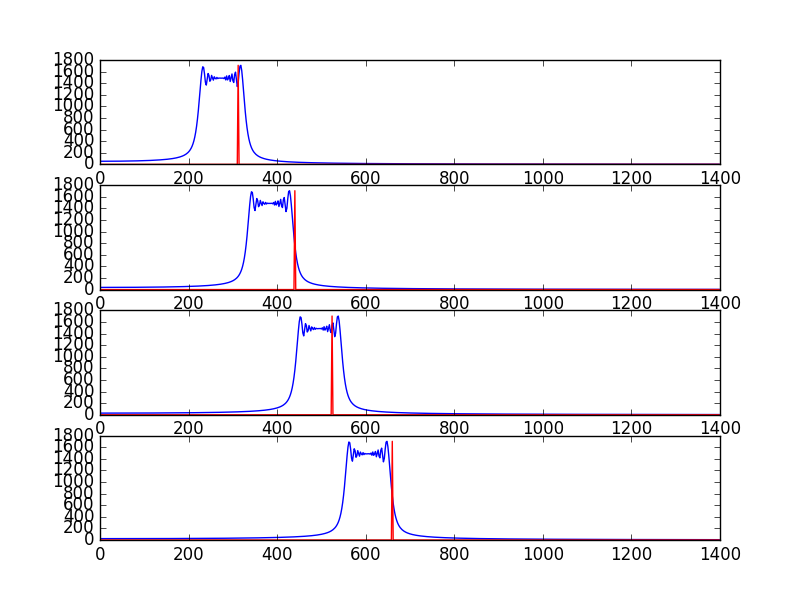
\includegraphics[width=0.7\textwidth]{images/autotune.png}


\subsection{Fourier in more than one dimensions}

\subsubsection{Mutliple input parameters}
Consider a simple black and white image. We'll describe the value at any pixel as $v(x, y)$, that is, $v: \reals^2 \to \reals$. Again, the base of the space of $(\reals^2 \to \reals)$ functions must consist of functions that are themselves $(\reals^2 \to \reals)$. The Fourier-representation of an image can be quite naturally obtained by: 


$$ v(x, y) = \sum_n^\infty \sum_m^\infty \alpha_{n,m} b_{n,m}(x, y) $$

where $b_{n,m}(x, y) = e^{i( \frac{n 2 \pi}{b_x - a_x} x + \frac{m 2 \pi}{b_y - a_y} y)}$ and  

$$ \alpha_{n,m} = \int_{a_x}^{b_x} \int_{a_y}^{b_y} v(x, y) e^{i( \frac{n 2 \pi}{b_x - a_x} x + \frac{m 2 \pi}{b_y - a_y} y)} \diff{y} \diff{x}$$

Generally, when a function takes two parameters, here $x,y$, then we also need two frequency parameters, here $n,m$. Analogously, for functions of three parameters we'd need three frequency parameters.


\subsubsection{Multiple output parameters: Vector valued functions}
In the previous section, we dealt with the space of functions mapping $\reals^2 \to \reals$. How about vector valued functions? Finally, we have arrived at the top level of abstraction when it comes to Fourier representations: the space of functions mapping $\reals^a \to \reals^b$. 

For example, consider the surface $\{ \vec{v} | v_z = v_x^2 + 3 v_y \}$. The set-expression can be rewritten into a function-expression: 

$$\vec{v}(x,y) = 
\begin{bmatrix} 
x \\
y \\
x^2 + 3 y
\end{bmatrix}$$

Here, we have an equation with two parameters ($v_x$ and $v_y$) mapping onto a 3d-vector $\vec{v}$. Consequently, the Fourier base of the space of surfaces, too, must consist of funcitons mapping $\reals^2 \to \reals^3$. 

As another example, consider an ellipsoid $\{\vec{v} | \frac{x^2}{r_1^2} + \frac{z^2}{r_2^2} + \frac{z^2}{r_3^2} = 1 \}$. This body can be parameterized as: 

$$ \begin{bmatrix}
x \\
y \\
z
\end{bmatrix} = 
\begin{bmatrix}
r_1 \cos{\theta} \cos{\phi} \\
r_2 \cos{\theta} \sin{\phi} \\
r_3 \sin{\theta}
\end{bmatrix} $$

This means we can represent the ellipsoid function as a sum of Fourier-base functions that map $[0\degree, 360\degree]^2 \to \reals^3$.

In general, we can represent any function mapping $\reals^a \to \reals^b$ by a Fourier base of functions from the same space. As for geometric bodies: as long as we can find a parameterisation of the body (that is continuous and sqare-integrable), we can also find a Fourier-representation\footnote{We cannot find a Fourier-representation of non-parameterisable sets. The reason for this is that sets don't form an inner-product space - or at least not without some whacky definitions.}. 

Surprisingly, this works just the same. Consider the ellipsoid in its parameterized representation: 

$$ \vec{v}(\phi, \theta) = 
\begin{bmatrix} 
    r_x \cos{\phi} \cos{\theta} \\
    r_y \cos{\phi} \sin{\theta} \\
    r_z \sin{\phi}
\end{bmatrix}  $$

$\vec{v}(\phi, \theta)$ is a member of the space $S = \{f: \reals^2 \to \reals^3\}$, so the basis must consist of functions of the same shape. Let's call one of the members of the basis $\vec{b}_{n,m}$. It must have the following structure: 

$$
\vec{b}_{n,m}(\phi, \theta) = 
\begin{bmatrix}
    b_{n,m}^x(\phi, \theta) \\
    b_{n,m}^y(\phi, \theta) \\
    b_{n,m}^z(\phi, \theta)
\end{bmatrix}
$$

Then the coefficient $\alpha_{n,m}$ is calculated like this: 

$$ \alpha_{n,m} = \int_{a_\theta}^{b_\theta} \int_{a_\phi}^{b_\phi} \vec{v}(\phi, \theta) \vec{b}_{n,m}(\phi, \theta) \diff{\phi} \diff{\theta} $$

$$ = \int_{a_\theta}^{b_\theta} \int_{a_\phi}^{b_\phi} (\vec{i} v^x(\phi, \theta) + \vec{j} v^y(\phi, \theta) \vec{k} v^z(\phi, \theta)) (\vec{i} b_{n,m}^x(\phi, \theta) + \vec{j} b_{n,m}^y(\phi, \theta) \vec{k} b_{n,m}^z(\phi, \theta)) \diff{\phi} \diff{\theta} $$

$$ = \int_{a_\theta}^{b_\theta} \int_{a_\phi}^{b_\phi} 1 v^x(\phi, \theta) b_{n,m}^x(\phi, \theta) + 0 + 0 + 0 + 1 v^y(\phi, \theta) b_{n,m}^y(\phi, \theta) + 0 + 0 + 0 + v^z(\phi, \theta) b_{n,m}^z(\phi, \theta) \diff{\phi} \diff{\theta} $$

$$ = \int_{a_\theta}^{b_\theta} \int_{a_\phi}^{b_\phi} v^x(\phi, \theta) b_{n,m}^x(\phi, \theta) \diff{\phi} \diff{\theta} + 
    \int_{a_\theta}^{b_\theta} \int_{a_\phi}^{b_\phi} v^y(\phi, \theta) b_{n,m}^y(\phi, \theta) \diff{\phi} \diff{\theta} + 
    \int_{a_\theta}^{b_\theta} \int_{a_\phi}^{b_\phi} v^z(\phi, \theta) b_{n,m}^z(\phi, \theta) \diff{\phi} \diff{\theta}  
$$

Let's apply the Fourier base $
\begin{bmatrix}
    b_{n,m}^x(\phi, \theta) \\
    b_{n,m}^y(\phi, \theta) \\
    b_{n,m}^z(\phi, \theta)
\end{bmatrix}
=
\begin{bmatrix}
    e^{i(\frac{n 2 \pi}{b_\phi - a_\phi}\phi + \frac{m 2 \pi}{b_\theta - a_\theta} \theta)} \\
    e^{i(\frac{n 2 \pi}{b_\phi - a_\phi}\phi + \frac{m 2 \pi}{b_\theta - a_\theta} \theta)} \\
    e^{i(\frac{n 2 \pi}{b_\phi - a_\phi}\phi + \frac{m 2 \pi}{b_\theta - a_\theta} \theta)} 
\end{bmatrix}
$ and the ellipsoid formula to this general expression. Then we get: 

$$ \alpha_{n,m} =   \int_{a_\theta}^{b_\theta} \int_{a_\phi}^{b_\phi} r_x \cos{\phi} \cos{\theta} e^{i(\frac{n 2 \pi}{b_\phi - a_\phi}\phi + \frac{m 2 \pi}{b_\theta - a_\theta} \theta)} \diff{\phi} \diff{\theta} + \\
                    \int_{a_\theta}^{b_\theta} \int_{a_\phi}^{b_\phi} r_y \cos{\phi} \sin{\theta} e^{i(\frac{n 2 \pi}{b_\phi - a_\phi}\phi + \frac{m 2 \pi}{b_\theta - a_\theta} \theta)} \diff{\phi} \diff{\theta} + \\
                    \int_{a_\theta}^{b_\theta} \int_{a_\phi}^{b_\phi} r_z \sin{\phi}              e^{i(\frac{n 2 \pi}{b_\phi - a_\phi}\phi + \frac{m 2 \pi}{b_\theta - a_\theta} \theta)} \diff{\phi} \diff{\theta}   $$
                
$$ \alpha_{n,m} =   r_x \int_{0}^{2\pi} \int_{0}^{2\pi} \cos{\phi} \cos{\theta} e^{i(n\phi + m\theta)} \diff{\phi} \diff{\theta} + \\
                    r_y \int_{0}^{2\pi} \int_{0}^{2\pi} \cos{\phi} \sin{\theta} e^{i(n\phi + m\theta)} \diff{\phi} \diff{\theta} + \\
                    t_z \int_{0}^{2\pi} \int_{0}^{2\pi} \sin{\phi}              e^{i(n\phi + m\theta)} \diff{\phi} \diff{\theta}   $$
                    
                    
Integrating yields:

...

Of course, the whole point is to graph the thing: 

\begin{lstlisting}[language=python]
import numpy as np

def ellipsoid(theta, phi, rx, ry, rz):
    x = rx * np.cos(theta) * np.cos(phi)
    y = ry * np.cos(theta) * np.sin(phi)
    z = rz * np.sin(theta)
    return x, y, z


def filterAmps(data, perc=0.8):
    dataAbs = np.abs(data)
    x, y = np.shape(data)
    thrsh = perc * np.max(dataAbs)
    filtered = np.zeros((x,y), dtype=np.complex128)
    for c in range(x):
        for r in range(y):
            if dataAbs[c,r] >= thrsh:
                filtered[c,r] = data[c,r]
    return filtered


def addOvertones(amps):
    x, y = np.shape(amps)
    ampsNew = np.zeros( (x, y), dtype=np.complex128 )
    for c in range(x): 
        for r in range(y):
            if np.abs(amps[c,r]) > 0:
                c2 = 2*c if 2*c < x else int(c/2)
                r2 = 2*r if 2*r < y else int(r/2)
                ampsNew[c,r] += amps[c,r]
                ampsNew[c,r2] += amps[c,r]
                ampsNew[c2,r] += amps[c,r]
                ampsNew[c2,r2] += amps[c,r]
    return ampsNew


rx = ry = rz = 1

data = np.zeros((360, 360, 3), dtype=np.float)
for t in np.arange(0,360):
    for p in np.arange(0, 360):
        data[t, p] = ellipsoid(t, p, rx, ry, rz)


ampsx = np.fft.rfft2(data[:,:,0])
ampsy = np.fft.rfft2(data[:,:,1])
ampsz = np.fft.rfft2(data[:,:,2])

ampsxF = filterAmps(ampsx, 0.001)
ampsyF = filterAmps(ampsy, 0.001)
ampszF = filterAmps(ampsz, 0.001)
ampsxF = addOvertones(ampsxF)
ampsyF = addOvertones(ampsyF)
ampszF = addOvertones(ampszF)

dataNew = np.zeros((360,360,3), dtype=np.float)
dataNew[:,:,0] = np.fft.irfft2(ampsxF)
dataNew[:,:,1] = np.fft.irfft2(ampsyF)
dataNew[:,:,2] = np.fft.irfft2(ampszF)
\end{lstlisting}


\begin{figure}[!htb]
\minipage{0.32\textwidth}
  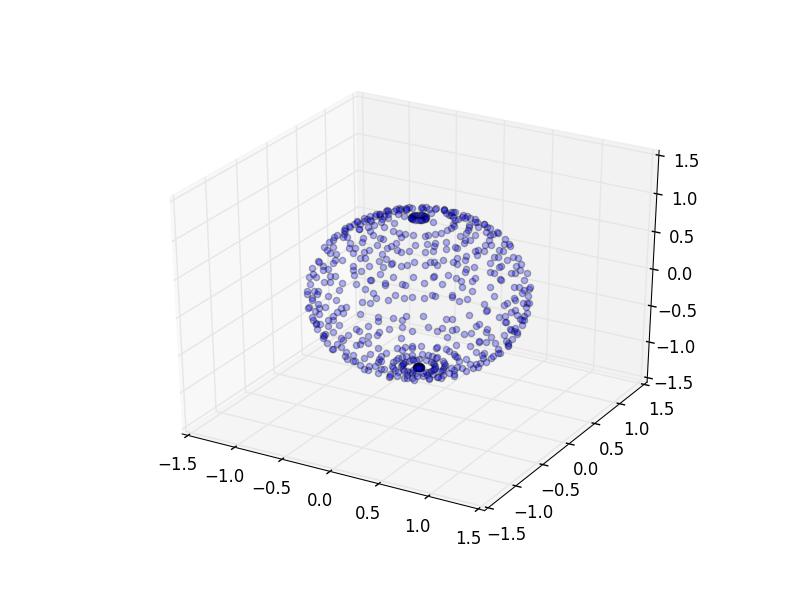
\includegraphics[width=\linewidth]{images/original_ellipsoid.png}
  \caption{Original ellipsoid}
\endminipage\hfill
\minipage{0.32\textwidth}
  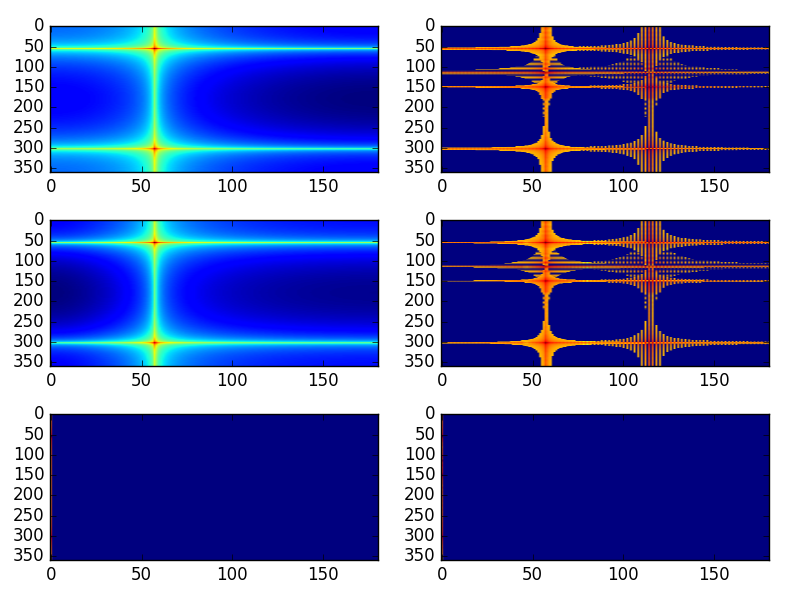
\includegraphics[width=\linewidth]{images/spectra_adjusted2.png}
  \caption{Left: original spectra, right: adjusted spectra}
\endminipage\hfill
\minipage{0.32\textwidth}%
  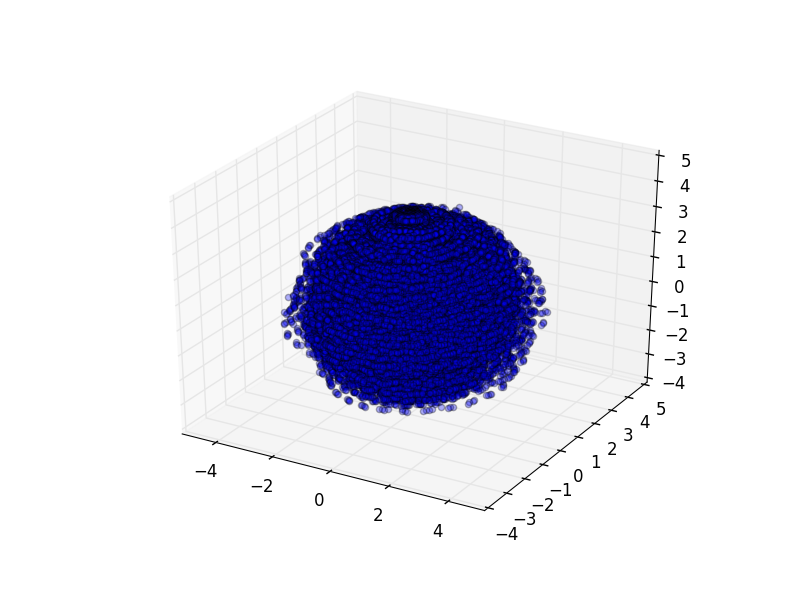
\includegraphics[width=\linewidth]{images/ellipsoid_backtransformed3.png}
  \caption{Ellipsoid backtransformed}
\endminipage
\end{figure}
\section{Estimating the time needed for a task}

\newcommand{\pois}{\ensuremath{\mathop{pois}}}
\newcommand{\tree}{\ensuremath{\mathop{tree}}}
\newcommand{\base}{\ensuremath{\mathop{base}}}
\newcommand{\child}{\ensuremath{\mathop{child}}}
\newcommand{\children}{\ensuremath{\mathop{children}}}
\newcommand{\GammaDist}{\ensuremath{\mathop{Gamma}}}
\newcommand{\var}{\ensuremath{\mathop{var}}}
\newcommand{\mean}{\ensuremath{\mathop{mean}}}


Lets model the growth of a tree like this: we begin with the trunk. From the trunk, branches may grow. How many branches is decided by a Poisson-distribution, whose expected number of branches is dependent on the height from the ground. 

\begin{lstlisting}[language=python]
from scipy.stats import poisson
from collections import namedtuple


Node = namedtuple('Node', 'parent, children')


def lamPerHeight(height):
    return 4 - height * 4 // 7


def randomTree(height=0):
    tree = Node(parent=None, children=[])
    lam = lamPerHeight(height)
    nrChildren = poisson.rvs(lam, size=1)
    for i in range(nrChildren):
        child = randomTree(height + 1)
        tree.children.append(child)
    return tree

print randomTree()
\end{lstlisting}

Using a Poisson-distribution, the probability of there being $k$ branches on height $h$ would be
$$ \pois_h(k) = \frac{ e^{-\lambda_h} \lambda_h^k }{ k! }$$

From the probability of a single branch we can now model the probabilty of a \tree. Consider the following \tree: 

\Tree[.n_1 [.n_2 n_3 ] n'_2 ] 

For this \tree the probability is $P(\tree) = \pois_1(2) \pois_2(1) \pois_3(0) \pois_2(0) $, or more generally:

$$ P(\tree) = \pois_1(|\children|) \prod_{\children} P(childtree)$$

\begin{lstlisting}[language=python]
def prob(tree, height=0):
    p = 1
    nrChildren = len(tree.children)
    lam = lamPerHeight(height)
    p *= poisson.pmf(nrChildren, lam)
    for child in tree.children:
        p *= prob(child, height + 1)
    return p


t = randomTree()
pt = prob(t)
\end{lstlisting}

Now what about this tree: 

\Tree[.n_1 [.n_2 [.n_3 ? ] ? ] [.n'_2 ? ] ? ] 

This is an unfinished tree. It's probability is $P(\{\tree | \tree_0 \subseteq \tree\}) = \pois_1(\geq2) \pois_2(\geq1) \pois_3(\geq0) \pois_2(\geq0) = \pois_1(\geq2) \pois_2(\geq1)$, or more generally: 

$$  P(\{\tree | \tree_0 \subseteq \tree\}) = \pois_1(\geq |\children|) \prod_{\children} P(\{ childtree | childtree_0 \subseteq childtree \}) $$

\begin{lstlisting}[language=python]
def probUnfinished(tree, height=0):
    p = 1
    nrChildren = len(tree.children)
    lam = lamPerHeight(height)
    p *= (1 - poisson.cdf(nrChildren, lam))
    for child in tree.children:
        p *= probUnfinished(child, height + 1)
    return p
\end{lstlisting}

\begin{figure}
  \caption{Using this model, we can spawn random trees}
  \centering
    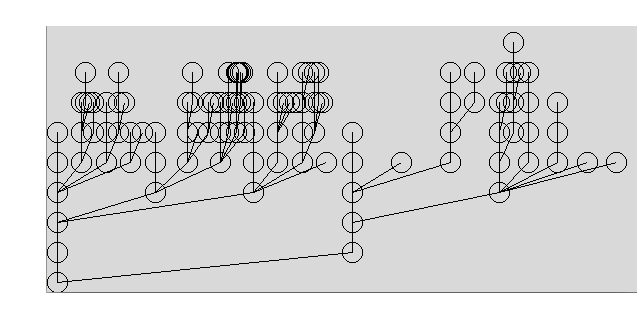
\includegraphics[width=0.5\textwidth]{images/randomtree.png}
\end{figure}

\paragraph{Time as random variable} 

Let time $T$ be a random variable of a tree $\tree$ defined as: 

$$ T_b(\tree) = T_n(\base) + \sum T_b(\child) $$

The expexted time for a not yet grown tree would then be:

$$ E[T_b] = \sum_{\tree \in \samplespace} T_b(\tree) P(\tree) $$

And the expected time given that we already have the fist few nodes of a tree:

$$ E[T_b]_{| \tree_0}  = \sum_{\tree \in \samplespace} T_b(\tree) P( \tree | \tree_0 )$$

This sum is pretty hard to compute, since \samplespace is an infinite set. But there is a way around this problem. Consider this tree: 

\Tree [.n_1 [.n_2 n_3 ] n'_2 ]

What is the expected number $k$ of nodes on level 2, given that there are already two offspring? 

$$ E[k] | k \geq 2 = \sum_{k=0}^\infty k P(k|2) =  \sum_{k=2}^\infty k \frac{ \pois_{\lambda_2}(k) }{ \pois_{\lambda_2}(\geq 2) }$$

$$ = \frac{1}{\pois_{\lambda_2}(\geq 2)} [ \sum_{k=0}^\infty k \pois_{\lambda_2}(k)  - \sum_{k=0}^1 k \pois_{\lambda_2}(k) ] $$

$$ = \frac{1}{\pois_{\lambda_2}(\geq 2)} [ E[k] - \sum_{k=0}^1 k \pois_{\lambda_2}(k) ]$$

$$ = \frac{\lambda - \sum_{k=0}^{k=1} k \pois_{\lambda_2}(k)}{1 - \sum_{k=0}^{k=1} \pois_{\lambda_2}(k)}$$

$$ = \frac{ \lambda - e^{-\lambda} \sum_{k=0}^{k=1} k \lambda^k / k! }{ 1 - e^{-\lambda} \sum_{k=0}^{k=1} \lambda^k / k! } $$


We can check our predictions numerically: 

\begin{lstlisting}[language=python]
from math import factorial, exp, floor


def pois(lmbd, k):
    return exp(-lmbd) * lmbd**k / factorial(k)


def poisCuml(lmbd, k):
    p = 0
    for j in range(k+1):
        p += pois(lmbd, j)
    return p


def poisCond(lmbd, k, k0):
    pb = 1 - poisCuml(lmbd, k0 - 1)
    if k < k0:
        pa = 0
    else:
        pa = pois(lmbd, k)
    return pa / pb


def expPois(lmbd):
    s = 0
    for i in range(int(50*lmbd)):
        s += i * pois(lmbd, i)
    return s


def expPoisCond(lmbd, k0):
    e = 0
    for i in range(k0, int(50*lmbd)):
        e += i * poisCond(lmbd, i, k0)
    return e


def expPoisCondAnal(lmbd, k0):
    sum1 = sum2 = 0
    for k in range(k0 + 1):
        sum1 += k * lmbd**k / float(factorial(k))
    for k in range(k0 + 1):
        sum2 += lmbd**k / float(factorial(k))
    sum1 *= exp(-lmbd)
    sum2 *= exp(-lmbd)
    a = float(lmbd - sum1)
    b = float(1 - sum2)
    return a / b

\end{lstlisting}


We will make use of this result shortly.

\begin{figure}
  \caption{When we already have 6 nodes, the probability of getting new nodes changes}
  \centering
    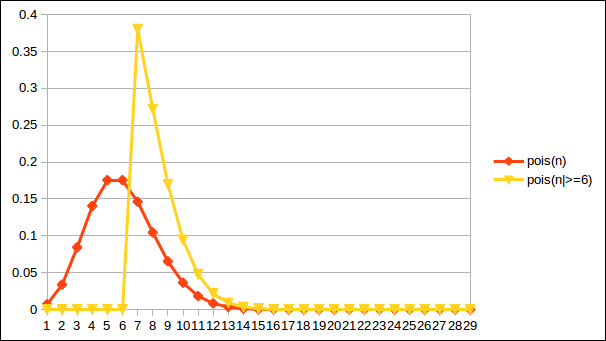
\includegraphics[width=0.5\textwidth]{images/conditional_poisson.png}
\end{figure}





We can use this to find an intuitive expression for $E[T_b(\tree)]$, which would be: 

$$ E[T_b(\tree)]_{| \tree_0} = E[T_n(\base) + \sum T_b(\child)]_{| \tree_0} $$

$$ = E[T_n(\base)]_{| \tree_0} + E[ \sum T_b(\child) ]_{| \tree_0} $$

The term $ E[ \sum T_b(\child) ]_{| \tree_0} $ is somewhat special: we cannot just equal it to $  \sum E[ T_b(\child) ]_{|\tree_0} $, because we don't yet know how many children the tree will have. But it is reasonable to assume that:

$$ E[ \sum T_b(\child) ]_{| \tree_0} = \sum_{children_0} E[T_b(\child)] + \sum_{E[|\children|]_{ \children_0} - \children_0} E[T_b(\child)] $$

With this, the previous equation becomes: 

$$ E[T_b(\tree)]_{| \tree_0} = E[T_n(\base)]_{| \tree_0} +  \sum_{\children_0} E[T_b(\child)] + \sum_{E[|\children|]_{ \children_0} - \children_0} E[T_b(\child)] $$

Now there are a bunch of terms in this equation that we can approximate statistically: 

\begin{itemize}

    \item $ E[|\children|]_{| \children_0} = \frac{ \lambda - e^{-\lambda} \sum_{k=0}^{k=\children_0 - 1} k \lambda^k / k! }{ 1 - e^{-\lambda} \sum_{k=0}^{k=\children_0 - 1} \lambda^k / k! }  $. Here we can approximate $\lambda$ by the average number of children on this level.
    
    \item $ E[T_n(\base)]_{| \tree_0} $ can be approximated by the average net-time on this level
    
    \item $ E[T_b(\child)] $ knows two cases: 
    
        \begin{itemize}
            
            \item if we're dealing with a real child, the value is approximated with the same formula applied recursively 
            
            \item if we're dealing with a not-yet-spawned child, we have: $ E[T_b] = E[T_n(1)] + E[\#c1] E[T_n(2)] + E[\#c1]E[\#c2]E[T_n(3)] + E[\#c1]E[\#c2]E[\#n3]E[T_n(4)] + ... $
        \end{itemize}

\end{itemize}


\paragraph{Time as random variable: revisited}

We can enhance our model quite a bit by recognizing that $T_b(\base)$ is not a constant, but a random variable in its own right. 

Then this random variable would still be defined as: 

$$ T_b(\tree) = T_n(\base) + \sum T_b(\child) $$

But $T_n(\base)$ itself would be random as well. 

Under these assumptions, we get: 

$$ P(t | t_0) = \{ \begin{array}{lr}
        \frac{P(t)}{1 - P(t<t_0)}       & \text{for } t \geq t_0 \\
        0                               & \text{for }  t < t_0
        \end{array}  $$

$$ E[T_n(\base)]_{|t_0} = \int_0^\infty t P(t|t\geq t_0) \diff{t} $$

$$ = \frac{1}{1 - P(t|t<t_0)} \int_{t_0}^\infty t P(t) \diff{t} $$

$$ = \frac{1}{1 - P(t|t<t_0)} [ E[t] - \int_0^{t_0} t P(t) \diff{t} ] $$

Assuming that $P(t) = \GammaDist_{\alpha,\beta}(t) = \frac{\beta^\alpha e^{-\beta} t^{\alpha-1} }{\Gamma(\alpha) } $, we obtain: 

$$ \int_0^{t_0} t P(t) \diff{t} = \frac{\beta^\alpha e^{-\beta} }{\Gamma(\alpha) } \int_0^{t_0} t^{\alpha - 1} t \diff{t} $$

$$ =  \frac{\beta^\alpha e^{-\beta} t_0^{\alpha-1} }{\Gamma(\alpha) }  \frac{t_0^2}{\alpha + 1} = \GammaDist_{\alpha, \beta}(t_0) \frac{t_0^2}{\alpha + 1} $$


Here, the parameters $\alpha$ and $\beta$ can be estimated by: 

$$ \alpha \approx \frac{\mean(t) \mean(t)}{\var(t)} $$
$$ \beta \approx \frac{\mean(t)}{\var(t)} $$


We can once again verify this model numerically: 

\begin{lstlisting}[language=python]
import scipy as sp
from scipy.stats import gamma
import matplotlib.pyplot as plt


def rateToScale(beta):
    return 1/beta

def scaleToRate(theta):
    return 1/theta

def probGamma(t, alpha, beta):
    theta = rateToScale(beta)
    return gamma.pdf(t, a=alpha, scale=theta)

def probGammaCond(t, t0, alpha, beta):
    theta = rateToScale(beta)
    gam = gamma(a=alpha, scale=theta)
    tpart1 = t[sp.where(t<t0)]
    outpart1 = sp.zeros(sp.shape(tpart1))
    tpart2 = t[sp.where(t>=t0)]
    pt = gam.pdf(tpart2)
    Pt0 = gam.cdf(t0)
    outpart2 = pt / (1 - Pt0 )
    return sp.concatenate([outpart1, outpart2])

def expGammaCond(t0, alpha, beta):
    theta = rateToScale(beta)
    gam = gamma(a=alpha, scale=theta)
    expv = gam.mean()
    gt0 = gam.pdf(t0)
    gfac = t0 * t0 / (alpha + 1)
    gCumt0 = gam.cdf(t0)
    return ( expv - gt0 * gfac ) / ( 1 - gCumt0 )

mean = 3.0
var = 2.0
alpha = mean * mean / var
beta = mean / var
t0  = 4
t = sp.arange(0, 10, 0.1)
pn = probGamma(t, alpha, beta)
pc = probGammaCond(t, t0, alpha, beta)


plt.plot(t, pn)
plt.plot(t, pc)
plt.show()
\end{lstlisting}


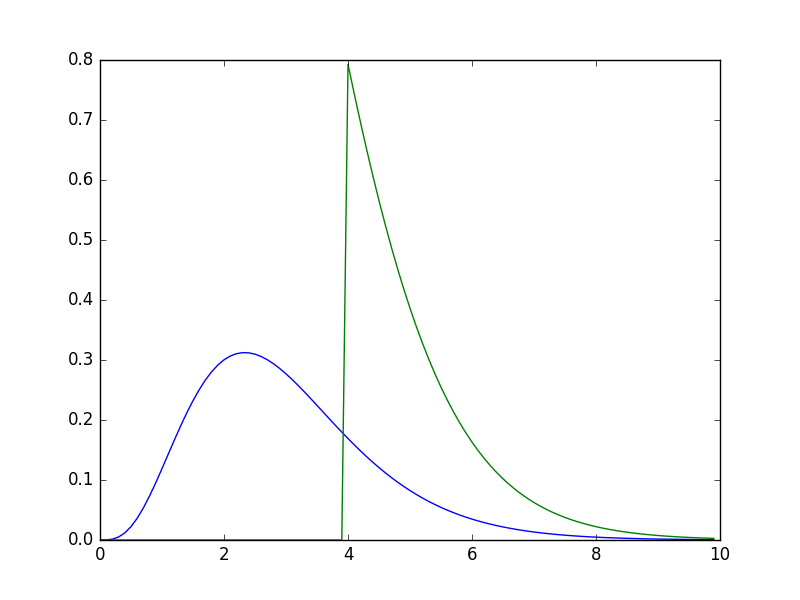
\includegraphics[width=0.5\textwidth]{images/beta_conditional.png}


This model justifies another look at our samplespace. Note that ....

\section{Scheduling}

The proposed algorithm is simple: 

\begin{enumerate}
    \item Take the most urgent remaining task $T_i$.
    \item Put it in the slot $[t_0, t_0 + expt(T_i)]$
    \item If $t_0 + expt(T_i) > deadline(T_i)$, throw an exception
    \item Set $t_0 = t_0 + expt(T_i)$ and $i = i+1$ and loop to step 1.
\end{enumerate}

Doublecheck: What if the task has scheduled subtasks?

\subsection{Running time}

\subsection{Partial correctness}

\subsection{Termination}


\section{Webcamgiant}

\subsection{Webcam to RPy}

\subsection{RPy to computer}

We need some way to transfer the images from the raspberry to our computer. Obviously, my favourite way would be over the internet - but to use the internet, you need a cable (ISDN or DSL) that is connected to some public router. Since we don't have that out in the field, we need to fall back onto a wireless transfer - GSM. 

\subsection{Computer to Oculus}


%\chapter{Fun Stuff}
%\section{Fun stuff}

Man kann nicht immer arbeiten. Hier eine Liste von anderen Dingen, die auch die Zeit wert sind:

\begin{itemize}
    \item Malen
    \item Lasertag
    \item Freizeitpark, Trampolinpark
    \item Freibad, Rutschenwelt
    \item Konzerte
    \item Schlittschuhlaufen
    \item Krimi-Dinner
\end{itemize}

\section{Wise stuff}

\begin{itemize}
    \item Feeling stupid is just like being afraid: 
        \begin{itemize}
            \item It's normal. The art lies in getting over it.
            \item If you don't feel it, you're not living to your potential.
        \end{itemize}
        
    \item Perfection is reached not when there is nothing more to add, but when there is nothing more to substract. - Antoine de Saint-Exupéry
    
    \item You can easily stay focused on your task, not by power of will, but by understanding that you don't need to do any of those distracting things, and that they won't make you happy.
    
    \item It is smart to realize when you need a break and how to take it. Knowing that teaches you to listen to your body and to your needs. Take a break early. On the break, don't do anything that strains your mind any further, but relax.
    
    \item Don't take yourself or anyone else too seriously. Remember that deep down you are goof, and anyone else is, too. That is the key to humor and charisma. 
    
    \item a tiny skill perfected beats a lage skill half-baked. If it's too hard, just do one small peace of it, but that really well. Things that you learned only mediocarily will stay bad permanently.  
    
    \item Comradery: 
        \begin{itemize}
            \item Requires organisation: keeping promises and not giving them too easily. Why do you not keep your promises? It feels like you don't live comradery. Strangely, comradery requires quite some level of organisation. You should only give promises when you have a good chance of keeping them. That requires a good organizer. 
            \item Requires social insight: keep track of who acted which way towards you, whom you owe stuff, who has been reliable in the past, who can survive a day without you, who needs you the most right now. Why do you have such a hard time making decissions? When one option is not obviously better, often none really is. For example, in Belgium you had the chióice between visiting Fabi in Brussels or Robin in Antwerp. Under such circumstances you couldn't have made the right decission, because there was none. However, you can keep to guidelines. Comradery would be one.  
        \end{itemize}
    
    \item The only way you can follow through on your carreer is by making every day so that 
        \begin{itemize}
            \item you enjoy the day
                \begin{itemize}
                    \item when you don't like the current project, focus on the part that you do like
                \end{itemize}
            \item you get stuff done
                \begin{itemize}
                    \item by keeping a startup-attitude
                    \item we-all-work-for-each-other
                    \item i-learn-from-everyone-else
                    \item get more efficient every day
                \end{itemize}
        \end{itemize}
\end{itemize}

\chapter{Physics}
\section{Remote sensing}

\subsection{Electromagnetic radiation}


\subsection{Important satellites}

\subsubsection{Landsat}

\subsubsection{Sentinel}

\subsubsection{Modis}


\subsection{Important datasets (possibly cumulated from multiple satellites and on-site measurements)}

\subsubsection{CHIRPS}

\begin{appendices}
\section{Spring}

Spring is such a vast framework that it is worth its own section. 
In general the principle is as follows:

\begin{itemize}
    \item A main class starts the context. From the context, it starts the app.
    \item The context wires together all the loose beans of your model and your utils using a bean.xml
\end{itemize}

\subsection{Dependency injection}

A basic spring-app may be set up like this: 

\begin{lstlisting}[language=xml]
<dependencies>
	<dependency>
		<groupId>org.springframework</groupId>
		<artifactId>spring-context</artifactId>
		<version>4.3.10.RELEASE</version>
	</dependency>
</dependencies>
\end{lstlisting}

\begin{lstlisting}[language=java]
package model;

public interface Knight {
	public void embarkOnQuest();
}
\end{lstlisting}


\begin{lstlisting}[language=java]
package model;

public class BraveKnight implements Knight {

	private Quest quest;
	
	public BraveKnight(Quest quest) {
		this.quest = quest;
	}

	public void embarkOnQuest() {
		quest.embark();
	}
}
\end{lstlisting}


\begin{lstlisting}[language=java]
package model;

public interface Quest {
	public void embark();
}

\end{lstlisting}

\begin{lstlisting}[language=java]
package model;

public class DamselRescueQuest implements Quest {

	public void embark() {
		System.out.println("Knight will now rescue the damsel!");
	}

}
\end{lstlisting}


\begin{lstlisting}[language=java]
package model;

public class DragonSlayingQuest implements Quest {

	public void embark() {
		System.out.println("Knight will now slay the dragon!");
	}

}

\end{lstlisting}

\begin{lstlisting}[language=java]
package main;

import org.springframework.context.annotation.Bean;
import org.springframework.context.annotation.ComponentScan;
import org.springframework.context.annotation.Configuration;

import model.BraveKnight;
import model.DamselRescueQuest;
import model.Knight;
import model.Quest;

@Configuration
@ComponentScan("model")
public class KnightsConfig {

	@Bean
	public Knight knight() {
		return new BraveKnight(quest());
	}
	
	@Bean
	public Quest quest() {
		return new DamselRescueQuest();
	}
}
\end{lstlisting}


Annotations: 
\begin{itemize}
    \item Configuration: Use this class instead of a xml file for the wiring-instructions
    \item ComponentScan: look in these packages to scan for beans
    \item Bean: put this object in the spring context. By default, the bean will be given an ID that is the same as the @Bean-annotated method’s name.
\end{itemize}

\begin{lstlisting}[language=java]
package main;

import org.springframework.context.annotation.AnnotationConfigApplicationContext;

import model.Knight;

public class AppMain {

	public static void main(String[] args) {
		AnnotationConfigApplicationContext acac = new AnnotationConfigApplicationContext(KnightsConfig.class);
		
		Knight k = acac.getBean(Knight.class);
		k.embarkOnQuest();
		
		acac.close();
	}
}
\end{lstlisting}


As you can see, the basic idea is this: 
Use a DI framework to ensure that all beans are maximally decoupled and easily interchangeable.


\subsection{Aspects}

Aspects allow you to keep utility objects, like logging, authentication, security, etc out of your model. 

\begin{lstlisting}[language=xml]
<dependencies>
	<dependency>
		<groupId>org.springframework</groupId>
		<artifactId>spring-context</artifactId>
		<version>4.3.10.RELEASE</version>
	</dependency>

	<dependency>
		<groupId>org.springframework</groupId>
		<artifactId>spring-aop</artifactId>
		<version>4.3.10.RELEASE</version>
	</dependency>

	<dependency>
		<groupId>org.springframework</groupId>
		<artifactId>spring-aspects</artifactId>
		<version>4.3.10.RELEASE</version>
	</dependency>
</dependencies>
\end{lstlisting}

\begin{lstlisting}[language=java]
package util;

import java.io.PrintStream;

public class Minstrel {
	
	private PrintStream stream;

	public Minstrel(PrintStream stream) {
		this.stream = stream;
	}
	
	public void singBeforeQuest() {
		stream.println("Fa la la la, the knight is so brave!");
	}
	
	public void singAfterQuest() {
		stream.println("Tee hee hee, the brave knight did finish the quest!");
	}
}
\end{lstlisting}

\begin{lstlisting}[language=xml]
<?xml version="1.0" encoding="UTF-8"?>

<beans xmlns="http://www.springframework.org/schema/beans"
	xmlns:xsi="http://www.w3.org/2001/XMLSchema-instance" 
	xmlns:aop="http://www.springframework.org/schema/aop"
	xsi:schemaLocation="http://www.springframework.org/schema/aop
http://www.springframework.org/schema/aop/spring-aop-3.2.xsd
http://www.springframework.org/schema/beans
http://www.springframework.org/schema/beans/spring-beans.xsd">

	<bean id="knight" class="model.BraveKnight">
		<constructor-arg ref="quest"></constructor-arg>
	</bean>

	<bean id="quest" class="model.DamselRescueQuest">
	</bean>

	<bean id="minstrel" class="util.Minstrel">
		<constructor-arg value="#{T(System).out}"></constructor-arg>
	</bean>

	<aop:config>
		<aop:aspect ref="minstrel">
			<aop:pointcut id="embark" expression="execution(* *.embarkOnQuest(..))" />
			<aop:before pointcut-ref="embark" method="singBeforeQuest" />
			<aop:after pointcut-ref="embark" method="singAfterQuest" />
		</aop:aspect>
	</aop:config>

</beans>
\end{lstlisting}


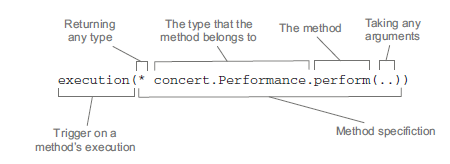
\includegraphics[width=8cm]{images/pointcut.png}

We put the knights.xml in src/main/resources. This is because files are loaded from the classpath, that is, the root of the produced jar. And resources is always put right into the root of the jar. 

\begin{lstlisting}[language=java]
package main;

import org.springframework.context.annotation.AnnotationConfigApplicationContext;
import org.springframework.context.support.ClassPathXmlApplicationContext;

import model.Knight;

public class AppMain {

	
	public static void main(String[] args) {
		ClassPathXmlApplicationContext ctx = new ClassPathXmlApplicationContext("knights.xml");

		Knight k = ctx.getBean(Knight.class);
		k.embarkOnQuest();
		
		ctx.close();
	}
}
\end{lstlisting}




Some jargon knowledge is in order:
\begin{itemize}
    \item advice: the action taken by an aspect. In the above example, \inlinecode{println}. Spring knows five kinds of advice: before, after, after-returning, after-throwing, and around.
    \item join-points: moments in the spring workflow where a advice may be applied. Internally, spring here loops through all registered aspects and checks if any of them applies in the given situation. (Equivalent to places where hooks are looped through in drupal.) In other words: any place in spring where \emph{some} aspect \emph{might} be applied. 
    \item pointcuts: a subset of all join-points, where \emph{an actual} aspect \emph{is} applied.
    \item introduction: An introduction allows you to add new methods or attributes to existing classes. For
    example, you could create an Auditable advice class that keeps the state of when an object was last modified. This could be as simple as having one method, setLast-Modified(Date), and an instance variable to hold this state. The new method and instance variable can then be introduced to existing classes without having to change them, giving them new behavior and state.
\end{itemize}

Aspects are woven in sometime during the execution of the application. Typically, an AOP container dynamically generates a proxy object that delegates to the target object while weaving in the aspects. This is how Spring AOP aspects are woven. However, JaspectJ can do this during compile-time!

You really don't need to use xml-configuration to be able to use aspects. We can also use the annotation-api borrowed from AspectJ: 

\begin{lstlisting}[language=java]
@Aspect
public class Audience {
	
	@Pointcut("execution(** concert.Performance.perform(..))")
	public void performance() {}

	@Before("performance()")
	public void silenceCellPhones() {
		System.out.println("Silencing cellphones");
	}
	
	@AfterThrowing("performance()")
	public void demandRefund() {
	System.out.println("Demanding a refund");
	}
}
\end{lstlisting}

Don't forget to tell spring that it should look for Aspects though!

\begin{lstlisting}[language=java]
@Configuration
@EnableAspectJAutoProxy
@ComponentScan
public class AppConfig {

	@Bean
	public Performance performance() {
		return new RollingStonesConcert();
	}
	
	@Bean
	public Audience audience() {
		return new Audience();
	}
}
\end{lstlisting}

\subsection{Templates}


\subsection{Bean lifecycle}
\begin{enumerate}
\item Spring instantiates the bean.
\item Spring injects values and bean references into the bean’s properties.
\item If the bean implements BeanNameAware, Spring passes the bean’s ID to the setBeanName() method.
\item If the bean implements BeanFactoryAware, Spring calls the setBeanFactory()
method, passing in the bean factory itself.
\item If the bean implements ApplicationContextAware, Spring calls the setApplicationContext() method, passing in a reference to the enclosing application
context.
\item If the bean implements the BeanPostProcessor interface, Spring calls its postProcessBeforeInitialization() method.
\item If the bean implements the InitializingBean interface, Spring calls its afterPropertiesSet() method. Similarly, if the bean was declared with an initmethod,
then the specified initialization method is called.
\item If the bean implements BeanPostProcessor, Spring calls its postProcessAfterInitialization() method.
\item At this point, the bean is ready to be used by the application and remains in the
application context until the application context is destroyed.
\item If the bean implements the DisposableBean interface, Spring calls its
destroy() method. Likewise, if the bean was declared with a destroy-method,
the specified method is called.
\end{enumerate}

By default, all beans in Spring are singletons.

\subsection{Wireing}

There are three ways of letting spring wire your components. 
\begin{enumerate}
\item Automatically using annotations. Pro: simple. Con: you cannot set @Component or @Autowire in external libraries.\marginpar{@Autowire is bad anyway, because it fails when there are more than one implementations to pick from. However, if there is only one implementation, then we don't need DI in the first place!}
\item With a Java @Configuration class. Pro: it's java. Con: You might be tempted to put business logic in the configuration. 
\item With xml. Pro: xml has one and only one purpose: config. Con: You cannot use any logic in your wireing.
\end{enumerate}


\subsection{Mocking}



\subsection{Spring MVC}

A spring-mvc app can be created in the same folder structure as any other eclipse java app.

The app consists really only of three parts: 
\begin{itemize}
    \item the servlet-container - usually a embeded tomcat. 
    \item the servlet, known as the dispatcher servlet
        \begin{itemize}
            \item configured with 
            \item redirects all requests to \inlinecode{@Controller}'s
        \end{itemize}
    \item the ContextLoaderListener
        \begin{itemize}
            \item reads the spring configuration-file
            \item creates spring-context
            \item creates web-application-context
        \end{itemize}
\end{itemize}

There are a few basic elements to every mvc-app: 

\begin{itemize}
    \item @Component: generic stereotype for any Spring-managed component
    \item @Repository: stereotype for persistence layer (jdbc, jpa, ...)
    \item @Service: stereotype for service layer (anything between controller and persistance layer)
    \item @Controller
\end{itemize}

Don't be afraid to use these annotations. Contrary to the general case, those mark classes that can only be part of a spring mvc app. It doesn't make sense to share them with other apps, so we might as well litter them with annotations.



\subsubsection{General structure}

Generally, every \inlinecode{@Controller} gets requests based on the rules defined in the \inlinecode{@RequestMapping}. The result of a request to a controller is always a string of a view-name. 

\subsubsection{Configuration}

\begin{itemize}
    \item AppInitializer: extends \inlinecode{AbstractAnnotationConfigDispatcherServletInitializer}. An alternative to the traditional web.xml file. Provides two configuration-classes: The servlet-config and the root-config. 
    
    \item Servlet-config: extends \inlinecode{WebMvcConfigurerAdapter}. The configuration for the servlet. 
    
    \item Root-config: the configuration for the backend, consisting of beans that are fully unaware of being used by a web-app. 
\end{itemize}

\subsubsection{Application: a minimal setup}

\begin{lstlisting}[language=xml,title=src/main/resources/appconfig]
<?xml version="1.0" encoding="UTF-8"?>

<beans xmlns="http://www.springframework.org/schema/beans"
       xmlns:xsi="http://www.w3.org/2001/XMLSchema-instance"
       xmlns:context="http://www.springframework.org/schema/context"
       xsi:schemaLocation="http://www.springframework.org/schema/beans
                           http://www.springframework.org/schema/beans/spring-beans.xsd
                           http://www.springframework.org/schema/context
                           http://www.springframework.org/schema/context/spring-context.xsd ">

    <context:component-scan base-package="sm" />

</beans>
\end{lstlisting}

\begin{lstlisting}[language=xml,title=src/main/resources/webconfig]
<?xml version="1.0" encoding="UTF-8"?>

<beans xmlns="http://www.springframework.org/schema/beans"
       xmlns:xsi="http://www.w3.org/2001/XMLSchema-instance"
       xmlns:context="http://www.springframework.org/schema/context"
       xmlns:mvc="http://www.springframework.org/schema/mvc"
       xsi:schemaLocation="http://www.springframework.org/schema/beans
                           http://www.springframework.org/schema/beans/spring-beans.xsd
                           http://www.springframework.org/schema/mvc
                           http://www.springframework.org/schema/mvc/spring-mvc.xsd
                           http://www.springframework.org/schema/context
                           http://www.springframework.org/schema/context/spring-context.xsd ">

	<context:component-scan base-package="sm" />

	<mvc:annotation-driven />
	<mvc:resources mapping="/resources/**" location="/resources/" />

	<bean class="org.springframework.web.servlet.view.InternalResourceViewResolver">
		<property name="viewClass" value="org.springframework.web.servlet.view.JstlView" />
		<property name="prefix" value="/WEB-INF/views/" />
		<property name="suffix" value=".jsp" />
	</bean>
	
</beans>
\end{lstlisting}

\begin{lstlisting}[language=xml,title=src/main/webapp/WEB-INF/web.xml]
<?xml version="1.0" encoding="UTF-8"?>

<web-app xmlns="http://xmlns.jcp.org/xml/ns/javaee"
         xmlns:xsi="http://www.w3.org/2001/XMLSchema-instance"
         xsi:schemaLocation="http://xmlns.jcp.org/xml/ns/javaee
                             http://xmlns.jcp.org/xml/ns/javaee/web-app_3_1.xsd" version="3.1">


    <context-param>
        <param-name>contextConfigLocation</param-name>
        <param-value>classpath:appconfig.xml</param-value>
    </context-param>

    <listener>
        <listener-class>org.springframework.web.context.ContextLoaderListener</listener-class>
    </listener>

    <servlet>
        <servlet-name>MyApp</servlet-name>
        <servlet-class>org.springframework.web.servlet.DispatcherServlet</servlet-class>
        <init-param>
            <param-name>contextConfigLocation</param-name>
            <param-value>classpath:webconfig.xml</param-value>
        </init-param>
        <load-on-startup>1</load-on-startup>
    </servlet>

    <servlet-mapping>
        <servlet-name>MyApp</servlet-name>
        <url-pattern>/</url-pattern>
    </servlet-mapping>

</web-app>
\end{lstlisting}


\begin{lstlisting}[language=java,title=src/main/java/sm/controller/AppMain.java]
package sm.controller;

import org.springframework.stereotype.Controller;
import org.springframework.ui.Model;
import org.springframework.web.bind.annotation.RequestMapping;
import org.springframework.web.bind.annotation.RequestMethod;

@Controller
@RequestMapping("/")
public class HomeController {

    @RequestMapping(method = RequestMethod.GET)
    public String index(Model model){
        model.addAttribute("message", "Spring MVC XML Config Example");
        return "index";
    }

}
\end{lstlisting}


\begin{lstlisting}[language=xml,title=src/main/webapp/WEB-INF/views/index.jsp]
<%@ page contentType="text/html;charset=UTF-8" language="java" %>
<html>
<head>
    <title>Spring MVC XML Configuration Example</title>
</head>
<body>
    ${message}
</body>
</html>
\end{lstlisting}

\subsubsection{Application: what goes into the root-config?}


I find that in practice nearly all of your non-trivial Spring MVC applications will require an application context (as opposed to only the spring MVC dispatcher servlet context). It is in the application context that you should configure all non-web related concerns such as:

\begin{itemize}
    \item Security
    \item Persistence
    \item Scheduled Tasks
\end{itemize}

To make this a bit more concrete, here's an example of the Spring configuration I've used when setting up a modern (Spring version 4.1.2) Spring MVC application. Personally, I prefer to still use a WEB-INF/web.xml file but that's really the only xml configuration in sight.

\begin{lstlisting}[language=xml, title=WEB-INF/web.xml]
<?xml version="1.0" encoding="UTF-8"?>
<web-app xmlns="http://xmlns.jcp.org/xml/ns/javaee" xmlns:xsi="http://www.w3.org/2001/XMLSchema-instance" xsi:schemaLocation="http://xmlns.jcp.org/xml/ns/javaee http://xmlns.jcp.org/xml/ns/javaee/web-app_3_1.xsd" version="3.1">

  <filter>
    <filter-name>openEntityManagerInViewFilter</filter-name>
    <filter-class>org.springframework.orm.jpa.support.OpenEntityManagerInViewFilter</filter-class>
  </filter>

  <filter>
    <filter-name>springSecurityFilterChain</filter-name>
    <filter-class>org.springframework.web.filter.DelegatingFilterProxy
    </filter-class>
  </filter>

  <filter-mapping>
    <filter-name>springSecurityFilterChain</filter-name>
    <url-pattern>/*</url-pattern>
  </filter-mapping>

  <filter-mapping>
    <filter-name>openEntityManagerInViewFilter</filter-name>
    <url-pattern>/*</url-pattern>
  </filter-mapping>

  <servlet>
    <servlet-name>springMvc</servlet-name>
    <servlet-class>org.springframework.web.servlet.DispatcherServlet</servlet-class>
    <load-on-startup>1</load-on-startup>
    <init-param>
      <param-name>contextClass</param-name>
      <param-value>org.springframework.web.context.support.AnnotationConfigWebApplicationContext</param-value>
    </init-param>
    <init-param>
      <param-name>contextConfigLocation</param-name>
      <param-value>com.company.config.WebConfig</param-value>
    </init-param>
  </servlet>

  <context-param>
    <param-name>contextClass</param-name>
    <param-value>org.springframework.web.context.support.AnnotationConfigWebApplicationContext</param-value>
  </context-param>

  <context-param>
    <param-name>contextConfigLocation</param-name>
    <param-value>com.company.config.AppConfig</param-value>
  </context-param>

  <listener>
    <listener-class>org.springframework.web.context.ContextLoaderListener</listener-class>
  </listener>

  <servlet-mapping>
    <servlet-name>springMvc</servlet-name>
    <url-pattern>/</url-pattern>
  </servlet-mapping>

  <session-config>
    <session-timeout>30</session-timeout>
  </session-config>

  <jsp-config>
    <jsp-property-group>
      <url-pattern>*.jsp</url-pattern>
      <scripting-invalid>true</scripting-invalid>
    </jsp-property-group>
  </jsp-config>

</web-app>
\end{lstlisting}

\begin{lstlisting}[language=java, title=WebConfig.java]
@Configuration
@EnableWebMvc
@ComponentScan(basePackages = "com.company.controller")
public class WebConfig {

  @Bean
  public InternalResourceViewResolver getInternalResourceViewResolver() {
    InternalResourceViewResolver resolver = new InternalResourceViewResolver();
    resolver.setPrefix("/WEB-INF/views/");
    resolver.setSuffix(".jsp");
    return resolver;
  }
}
\end{lstlisting}


\begin{lstlisting}[language=java, title=AppConfig.java]
@Configuration
@ComponentScan(basePackages = "com.company")
@Import(value = {SecurityConfig.class, PersistenceConfig.class, ScheduleConfig.class})
public class AppConfig {
  // application domain @Beans here...
}
\end{lstlisting}


\begin{lstlisting}[language=java, title=Security.java]
@Configuration
@EnableWebSecurity
public class SecurityConfig extends WebSecurityConfigurerAdapter {
  @Autowired
  private LdapUserDetailsMapper ldapUserDetailsMapper;

  @Override
    protected void configure(HttpSecurity http) throws Exception {
    http.authorizeRequests()
      .antMatchers("/").permitAll()
      .antMatchers("/**/js/**").permitAll()
      .antMatchers("/**/images/**").permitAll()
      .antMatchers("/**").access("hasRole('ROLE_ADMIN')")
      .and().formLogin();

    http.logout().logoutRequestMatcher(new AntPathRequestMatcher("/logout"));
    }

  @Autowired
    public void configureGlobal(AuthenticationManagerBuilder auth) throws Exception {
      auth.ldapAuthentication()
      .userSearchBase("OU=App Users")
      .userSearchFilter("sAMAccountName={0}")
      .groupSearchBase("OU=Development")
      .groupSearchFilter("member={0}")
      .userDetailsContextMapper(ldapUserDetailsMapper)
      .contextSource(getLdapContextSource());
    }

  private LdapContextSource getLdapContextSource() {
    LdapContextSource cs = new LdapContextSource();
    cs.setUrl("ldaps://ldapServer:636");
    cs.setBase("DC=COMPANY,DC=COM");
    cs.setUserDn("CN=administrator,CN=Users,DC=COMPANY,DC=COM");
    cs.setPassword("password");
    cs.afterPropertiesSet();
    return cs;
  }
}
\end{lstlisting}


\begin{lstlisting}[language=java, title=PersistenceConfig.java]
@Configuration
@EnableTransactionManagement
@EnableJpaRepositories(transactionManagerRef = "getTransactionManager", entityManagerFactoryRef = "getEntityManagerFactory", basePackages = "com.company")
public class PersistenceConfig {

  @Bean
  public LocalContainerEntityManagerFactoryBean getEntityManagerFactory(DataSource dataSource) {
    LocalContainerEntityManagerFactoryBean lef = new LocalContainerEntityManagerFactoryBean();
    lef.setDataSource(dataSource);
    lef.setJpaVendorAdapter(getHibernateJpaVendorAdapter());
    lef.setPackagesToScan("com.company");
    return lef;
  }

  private HibernateJpaVendorAdapter getHibernateJpaVendorAdapter() {
    HibernateJpaVendorAdapter hibernateJpaVendorAdapter = new HibernateJpaVendorAdapter();
    hibernateJpaVendorAdapter.setDatabase(Database.ORACLE);
    hibernateJpaVendorAdapter.setDatabasePlatform("org.hibernate.dialect.Oracle10gDialect");
    hibernateJpaVendorAdapter.setShowSql(false);
    hibernateJpaVendorAdapter.setGenerateDdl(false);
    return hibernateJpaVendorAdapter;
  }

  @Bean
  public JndiObjectFactoryBean getDataSource() {
    JndiObjectFactoryBean jndiFactoryBean = new JndiObjectFactoryBean();
    jndiFactoryBean.setJndiName("java:comp/env/jdbc/AppDS");
    return jndiFactoryBean;
  }

  @Bean
  public JpaTransactionManager getTransactionManager(DataSource dataSource) {
    JpaTransactionManager jpaTransactionManager = new JpaTransactionManager();
    jpaTransactionManager.setEntityManagerFactory(getEntityManagerFactory(dataSource).getObject());
    jpaTransactionManager.setDataSource(dataSource);
    return jpaTransactionManager;
  }
}
\end{lstlisting}


\begin{lstlisting}[language=java, title=ScheduleConfig.java]
@Configuration
@EnableScheduling
public class ScheduleConfig {
  @Autowired
  private EmployeeSynchronizer employeeSynchronizer;

  // cron pattern: sec, min, hr, day-of-month, month, day-of-week, year (optional)
  @Scheduled(cron="0 0 0 * * *")
  public void employeeSync() {
    employeeSynchronizer.syncEmployees();
  }
}
\end{lstlisting}

As you can see, the web configuration is only a small part of the overall spring web application configuration. Most web applications I've worked with have many concerns that lie outside of the dispatcher servlet configuration that require a full-blown application context bootstrapped via the org.springframework.web.context.ContextLoaderListener in the web.xml.


\subsection{Adding further servlets to spring mvc}




\subsection{Spring REST services}
Rest works just like SpingMvc. One single difference is that a controllers methods return types are not Strings with view names, but POJOs and annoted with \inlinecode{@ResponseBody}. The \inlinecode{@ResponseBody} annotation tells Spring MVC not to render a model into a view, but rather to write the returned object into the response body. It does this by using one of Spring’s message converters. Because Jackson 2 is in the classpath, this means that MappingJackson2HttpMessageConverter will handle the conversion of Greeting to JSON if the request’s Accept header specifies that JSON should be returned.

\subsection{Spring Database access}

\begin{lstlisting}[language=java]
@Bean
public JdbcTemplate jdbcTemplate(DataSource dataSource) {
    return new JdbcTemplate(dataSource);
}

@Bean
public DataSource dataSource() {
    return new EmbeddedDatabaseBuilder()
        .setType(EmbeddedDatabaseType.H2)
        .addScripts('schema.sql', 'data.sql')
        .build();
}
\end{lstlisting}
\section{Spring Boot}

Spring boot takes away a lot of the boilerplate from spring. It reads all your classes and wires them together mostly by itself.


\subsection{Example}
We can reimplement the knight example like this: 

\begin{lstlisting}[language=java, title=TtAplication]
@SpringBootApplication
public class TtApplication {
	public static void main(String[] args) {
		ConfigurableApplicationContext context = SpringApplication.run(TtApplication.class, args);
		Knight k = context.getBean(Knight.class);
		String result = k.goOnQuest();
		System.out.println(result);
	}
}
\end{lstlisting}

\begin{lstlisting}[language=java, title=TtConfig]
@Configuration
public class TtConfig {
	@Bean
	public Knight knight(Quest quest) {
		return new NotSoBraveKnight(quest);
	}
	@Bean 
	public Quest quest() {
		return new ScaryQuest();
	}
}
\end{lstlisting}

Running this results in \inlinecode{"The not-so-brave knight reluctantly goes on a quest to slay a dangerous dragon"}.



\subsection{Configuration}
Spring boot will automatically detect any classes marked with \inlinecode{@Configuration}  in your classpath.




\subsection{Database access}

You can create a Jpa instance by just creating an interface extending the interface \inlinecode{JpaRepository}.  Spring boot will automatically check your classpath for any jpa-provider and use that to create the actual implementation of the interface. 
If you don't want to use jpa, you can instead ...








\subsection{Websites}
Spring is primarily a framework for web-enabled apps. Consequently, spring boot makes developing webapps quite easily. 
First of all, we add two dependencies to our pom: \verb starter-web, starter-thymeleaf   and \verb devtools  . 
\begin{lstlisting}[language=xml]
  <parent>
		<groupId>org.springframework.boot</groupId>
		<artifactId>spring-boot-starter-parent</artifactId>
		<version>1.5.9.RELEASE</version>
	</parent>
  
  
  <!-- Add typical dependencies for a web application -->
	<dependencies>
		<dependency>
			<groupId>org.springframework.boot</groupId>
			<artifactId>spring-boot-starter-web</artifactId>
		</dependency>
		<dependency>
            <groupId>org.springframework.boot</groupId>
            <artifactId>spring-boot-starter-thymeleaf</artifactId>
        </dependency>
        <dependency>
            <groupId>org.springframework.boot</groupId>
            <artifactId>spring-boot-devtools</artifactId>
            <optional>true</optional>
        </dependency>
	</dependencies>

	<!-- Package as an executable jar -->
	<build>
		<plugins>
			<plugin>
				<groupId>org.springframework.boot</groupId>
				<artifactId>spring-boot-maven-plugin</artifactId>
			</plugin>
		</plugins>
	</build>
\end{lstlisting}

Now we need a main-class from where spring can run, a controller for the webrequests, and finally a file in the resources folder that contains the template.
\begin{lstlisting}[language=java]
@SpringBootApplication
public class Main {
    public static void main(String[] args) {
        SpringApplication.run(Main.class, args);
    }
}
\end{lstlisting}

\begin{lstlisting}[language=java]
@Controller
public class WebsiteMainController {
	
	@RequestMapping("/greeting")
	public String startSite( @RequestParam(value="name", required=false, defaultValue="World") String name, Model model) {
		model.addAttribute("name", name);
		return "greeting"; // name of the template html-file to be used
	}
}
\end{lstlisting}

Here is the template, situated in \verb src/main/resources/templates/greeting.html  .

\begin{lstlisting}[language=html]
<!DOCTYPE HTML>
<html xmlns:th="http://www.thymeleaf.org">
<head>
    <title>Getting Started: Serving Web Content</title>
    <meta http-equiv="Content-Type" content="text/html; charset=UTF-8" />
</head>
<body>
    <p th:text="'Hello, ' + ${name} + '!'" />
</body>
</html>
\end{lstlisting}

You can start the app with the command \inlinecode{mvn spring-boot:run}. Going to the url \verb localhost:8080/greeting?name=Michael  will show you the expected site. Spring will automatically detect all changes you make to the source, and then rebuild and restart the app. You can also build the app with \inlinecode{mvn clean package} and then run it with \inlinecode{java -jar target/myWebApp-1.0.jar}








\subsection{Testing}
For all your model classes, you can use the usual procedure of JUnit tests. But you might also want to test that spring itself is working fine. This section describes how to do this. 

First, add Testing-support as a dependency: 
\begin{lstlisting}
<dependency>
    <groupId>org.springframework.boot</groupId>
    <artifactId>spring-boot-starter-test</artifactId>
    <scope>test</scope>
</dependency>
\end{lstlisting}

Now you can create Tests. For spring stuff, we use two special annotations: \inlinecode{@RunWith} and \inlinecode{@SpringBootTest} (Tells the Testser to go look for a main configuration class (one with @SpringBootApplication for instance), and start spring from there).
\begin{lstlisting}
@RunWith(SpringRunner.class)
@SpringBootTest
public class MainTest {
	@Test
	public void contextLoads() throws Exception {
	}
}
\end{lstlisting}
Tests are run by simply calling \inlinecode{mvn test}.



\subsection{Camel}

Camel is quite easily integrated into spring boot. 

\begin{lstlisting}[language=java]
package org.langbein.michael.springcamel;

import org.springframework.boot.SpringApplication;
import org.springframework.boot.autoconfigure.SpringBootApplication;

@SpringBootApplication
public class SpringcamelApplication {

	public static void main(String[] args) {
		SpringApplication.run(SpringcamelApplication.class, args);
	}
}
\end{lstlisting}

\begin{lstlisting}[language=java]
package org.langbein.michael.springcamel.controllers;

import org.apache.camel.ProducerTemplate;
import org.springframework.beans.factory.annotation.Autowired;
import org.springframework.web.bind.annotation.RequestMapping;
import org.springframework.web.bind.annotation.RestController;

@RestController
public class CamelController {

	@Autowired
	ProducerTemplate producerTemplate;
	
	@RequestMapping(value="/")
	public void startCamel() {
		producerTemplate.sendBody("direct:firstRoute", "Calling via Spring Boot Rest Controller");
	}
}
\end{lstlisting}

\begin{lstlisting}[language=java]
package org.langbein.michael.springcamel.routes;

import org.apache.camel.builder.RouteBuilder;
import org.springframework.stereotype.Component;

@Component
public class CamelRoutes extends RouteBuilder {

	@Override
	public void configure() throws Exception {
		from("direct:firstRoute")
		.log("camel body: ${body}");
	}

	
}
\end{lstlisting}
\section{Android}


\subsection{ADB}
It really makes a lot of sense to use a physical phone instead of an emulated one. To be able to communicate with your phone, however, you need the adb-server to be aware of the phone. There is a commandline-tool, \verb adb, that you can use to have the adb-server talk to your phone. However, to be able to do that, you must first set up your phone accordingly. 
\begin{itemize}
    \item on your linux-machine, install \verb mtp-tools and \verb mtpfs . 
    \item mount your phone using a \emph{data} usb-cable
    \item enable developer-mode 
    \item have your phone use the MTP protocol
\end{itemize}
With that given, you should be able to see your phone with \inlinecode{lsusb} and \inlinecode{adb devices}.

\subsection{Basic concepts}

\paragraph{The structure of an app} is as follows: the compiled java-bytecode\footnote{actually, your code gets compiled to java-bytecode (i.e. several \verb .class files), but from there is is compiled on to a single \verb .DEX file to be run on androids version of the JRE, the ART.}, togehter with all libraries and resources, is packaged into an APK (android application package), analog to a jar or a war. 

\paragraph{The mainfest} mostly tells the phone some meta-info about the APK; like what rights are required, what SDK version is required, what the main-activity is, and such. 

\paragraph{A layout} describes the app's appearence on one screen. Written in XML. The layout can be found in \verb res/layout. Within a layout file, you can reference data from \verb res/values/strings.xml by using the string \verb "@string/app\_someStringName" .

\paragraph{An activity} is a single, defined thing that your user can do. Activities are usually associated with one screen. In code, an activity is represented by a single class extending the class \inlinecode{Activity}. It largely has the role of \emph{controller}, negotiating between the \emph{view.xml} and a custom-class-backend. All activities need to be declared in the manifest.

\paragraph{An intent} is a type of message that one activity can send to another. It can be used to start another activity within the same app or even in another app. It can even be broadcasted to all apps on the phone so that any app that might be able to handle the request may use it. 
Here is an example of how we might use an intent to switch to another activity: 
\begin{lstlisting}[language=java]
letsGoButton = (Button) findViewById(R.id.startGameButton);
letsGoButton.setOnClickListener(new View.OnClickListener() {
	public void onClick(View view) {
		Intent goToGameActivity = new Intent(MainActivity.this, PlayActivity.class);
		startActivity(goToGameActivity);
	}
});
\end{lstlisting}


\paragraph{A view} is a custom drawable thing, like buttons or menus. You create such a view when the predefined UI-elements don't suite your needs, like when you want to create an animation. You create a view by extending \inlinecode{View} and implementing \inlinecode{onDraw(Canvas canvas), onTouchEvent(MotionEvent event)}, etc.

\paragraph{The file R.java} is an automatically created file that android uses to keep track of the resources available to your app. For example, your activity will tell the phone to use the \verb activity_play.xml layout file by going \inlinecode{setContentView(R.layout.activity_play);} inside the \verb onCreate method. We can access things in \verb R very much like we can in the \verb DOM .




\subsection{Userinput}
Android apps behave very much like html forms. 

The steps are: 
\begin{itemize}
    \item The main-activity choses a layout (in this case, \inlinecode{activity_find_beer.xml}) that is to be displayed by using 
    \begin{lstlisting}
        protected void onCreate(Bundle savedInstanceState) {
            super.onCreate(savedInstanceState);
            setContentView(R.layout.activity_find_beer);
        }
    \end{lstlisting}
    
    \item The layout specifies which method to call in the activity when a button is pressed. A button can have an attribute \inlinecode{android:onClick:"onClickFindBeer"}
    
    \item A click now is passed trhough to the activity, calling the method \inlinecode{public void onClickFindBeer(View view) }. In this case, \inlinecode{view} refers to the button that was pressed. 
    
    \item Anywhere in the application logic, the activity can get a hold of any element of the layout by using \inlinecode{findViewById()} like this: 
    \begin{lstlisting}
    TextView brands = (TextView) findViewById(R.id.brands);
    brands.setText("Gottle of geer");
    \end{lstlisting}
\end{itemize}




\subsection{Activities}
This section handles activities in more detail. 
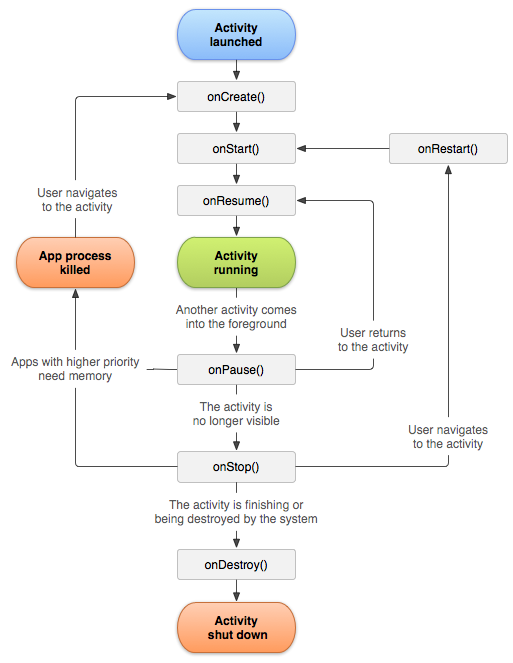
\includegraphics[scale=0.4]{images/activity_lifecycle.png}





\subsection{Threading}

\paragraph{Threads} come in three different flavors:

\begin{itemize}
    \item the main thread (aka. ui-thread)
        \begin{itemize}
            \item listens for intents
            \item listens for input (touch/speak) events
        \end{itemize}
    
    \item the render thread
        \begin{itemize}
            \item You don't normally interact with that thread. The main-thread passes it views to render, and the render thread executes the views \inlinecode{onDraw} methods. 
            \item However, you can steal work from it by creating a special kind of view: a \inlinecode{SurfaceView}. This kind of view exposes a canvas that is to be rendered in a custom thread.  
        \end{itemize}
        
    \item custom threads
        \begin{itemize}
            \item simple custom threads extending \inlinecode{Thread}
            \item android-specific custom threads extending \inlinecode{AsyncTask}
        \end{itemize}
\end{itemize}

\paragraph{Handlers} are a different thing than threads. They are not separate theads, they just postpone the execution of code. There basically promises: some code will be executed asynchronously, but sitll on the main thread. There are two usecases for handlers: 

\begin{itemize}
    \item You really want an action to happen on the main-thread, but at a later time. For example, ....
    \item Custom threads are not allowed to manipulate UI-elements on the main-thread. Instead, pass them a handler from the main-thread so they can call the handler. In other words: handlers are a (android-specific) method of inter-thread communication. 
\end{itemize}


\subsection{Drawing}
There are three ways of drawing in android apps. 
\begin{itemize}
    \item When you only need a single animated item in an overal static UI, draw your animations into a view.
    \item When you want your drawing to be updated regularly, use a canvas. 
    \item When you want to do 3d-rendering, use the OpenGL-API.
\end{itemize}


\paragraph{Using a custom view} is certainly the most straightforward way of creating graphics. Consider this simple example: 

\begin{lstlisting}[language=java]
public class PlayActivity extends AppCompatActivity {

    @Override
    protected void onCreate(Bundle savedInstanceState) {
        super.onCreate(savedInstanceState);
        setContentView(new FullScreenView(this));
    }
}
\end{lstlisting}

\begin{lstlisting}[language=java]
public class FullScreenView extends View {

    private Rect lilRect;
    private Paint painter;
    private static final int SQUARE_SIDE_LENGTH = 200;

    public FullScreenView(Context context) {
        super(context);
        lilRect = new Rect(30, 30, SQUARE_SIDE_LENGTH, SQUARE_SIDE_LENGTH);
        painter = new Paint();
        painter.setColor(Color.MAGENTA);
    }

    @Override
    protected void onDraw(Canvas canvas) {
        canvas.drawRGB(39, 111, 184);
        canvas.drawRect(lilRect, painter);
    }

    @Override
    public boolean onTouchEvent(MotionEvent event) {
        lilRect.left = (int) (event.getX() - (SQUARE_SIDE_LENGTH / 2));
        lilRect.right = (int) (event.getX() + (SQUARE_SIDE_LENGTH / 2));
        lilRect.top = (int) (event.getY() - (SQUARE_SIDE_LENGTH / 2));
        lilRect.bottom = (int) (event.getY() + (SQUARE_SIDE_LENGTH / 2));
        invalidate();
        return true;
    }
}
\end{lstlisting}


\paragraph{Using the canvas} is a lot more direct than using a view-object. We still make use of a custom view, but instead of calling \inlinecode{invalidate()} when we're ready to draw, we host the game-loop inside the view and act upon the canvas directly. 

\begin{lstlisting}
public class MainActivity extends AppCompatActivity {

    @Override
    protected void onCreate(Bundle savedInstanceState) {
        super.onCreate(savedInstanceState);
        SceneLogic boardScene = new BoardScene();
        MainView mainView = new MainView(this, boardScene);
        setContentView(mainView);
        mainView.startRenderThread();
    }
}
\end{lstlisting}

\begin{lstlisting}
/**
 * This class is there to present the SurfaceHolder as well as any touch- or system-events
 * to the RenderThread.
 */
public class MainView extends SurfaceView implements SurfaceHolder.Callback {

    private RenderThread renderThread;

    public MainView(Context context, SceneLogic sceneLogic) {
        super(context);
        SurfaceHolder surfaceHolder = getHolder();
        surfaceHolder.addCallback(this);
        renderThread = new RenderThread(context, surfaceHolder, sceneLogic);
    }

    public void startRenderThread() {
        renderThread.start();
    }

    public void stopRenderThread() {
        renderThread.setInactive();
    }

    @Override
    public boolean onTouchEvent(MotionEvent event) {
        return renderThread.getLogic().onTouch(event);
    }

    @Override
    public void surfaceCreated(SurfaceHolder surfaceHolder) {}

    @Override
    public void surfaceChanged(SurfaceHolder surfaceHolder, int i, int i1, int i2) {}

    @Override
    public void surfaceDestroyed(SurfaceHolder surfaceHolder) {}

}
\end{lstlisting}


\begin{lstlisting}
public class RenderThread extends Thread {

    private final long frameTime = 17;   // How long (in millisec) a frame may take
    private SceneLogic sceneLogic;
    private Context context;
    private SurfaceHolder surfaceHolder;
    private boolean running;

    public RenderThread(Context context, SurfaceHolder surfaceHolder, SceneLogic sceneLogic) {
        this.context = context;
        this.surfaceHolder = surfaceHolder;
        this.running = true;
        this.sceneLogic = sceneLogic;
    }

    @Override
    public void run() {
        long updateDuration = 0;
        long sleepDuration = 0;

        while(running) {

            // Step 0 : how long did the loop take?
            long beforeUpdateRender = System.nanoTime();
            long delta = sleepDuration + updateDuration;

            // Step 1 : scene logic
            sceneLogic.update(delta);

            // Step 2: scene rendering
            Canvas canvas = surfaceHolder.lockCanvas();
            if(canvas != null) {
                sceneLogic.draw(canvas);
                surfaceHolder.unlockCanvasAndPost(canvas);
            }

            // Step 3: sleep for remainder of frameTime
            updateDuration = (System.nanoTime() - beforeUpdateRender) / 1000000L;
            sleepDuration = Math.max(2, frameTime - updateDuration);
            try{
                Thread.sleep(sleepDuration);
            } catch (Exception e) {
                e.printStackTrace();
            }


        }
    }

    public SceneLogic getLogic() {
        return sceneLogic;
    }

    public void setInactive() {
        running = false;
    }
}
\end{lstlisting}





\section{C++ on android}
https://www.youtube.com/watch?v=zOsUZjWbudI&list=PL0C9C46CAAB1CFB2B&index=3



\section{VR on android}

\subsection{Basic app} 

\paragraph{The manifest} should basically be a variant of this: 
\begin{lstlisting}[language=xml]
<manifest ...
    <uses-permission android:name="android.permission.READ_EXTERNAL_STORAGE" />
    ...
    <uses-sdk android:minSdkVersion="19" android:targetSdkVersion="24"/>
    ...
    <uses-feature android:glEsVersion="0x00020000" android:required="true" />
    <uses-feature android:name="android.software.vr.mode" android:required="false"/>
    <uses-feature android:name="android.hardware.vr.high_performance" android:required="false"/>
    ...
    <application
            android:theme="@style/VrActivityTheme"
            ...
        <activity
                android:name=".TreasureHuntActivity
                ...
                android:screenOrientation="landscape"
                android:configChanges="orientation|keyboardHidden|screenSize|uiMode|navigation"
                android:enableVrMode="@string/gvr_vr_mode_component"
                android:resizeableActivity="false">
                ...

            <intent-filter>
                <action android:name="android.intent.action.MAIN" />
                <category android:name="android.intent.category.LAUNCHER" />
                <category android:name="com.google.intent.category.CARDBOARD" />
                <category android:name="com.google.intent.category.DAYDREAM" />
            </intent-filter>
        </activity>
    </application>
</manifest>
\end{lstlisting}

\paragraph{Gradle} handles the specific dependencies that are required to make a 3d-app. At least you're going to need: 
\begin{lstlisting}
allprojects {
    repositories {
        jcenter() // this is where we get the vr libraries
    }
}
model {
    android {
        ...
        buildTypes {
            release {
                minifyEnabled true
                // Progueard minifies the APK. This line makes sure it doesn't obfuscate vr-libs.
                proguardFiles.add(file('../../proguard-gvr.txt'))
            }
        }
    }
}
dependencies {
    classpath 'com.android.tools.build:gradle:2.3.3'
    compile 'com.google.vr:sdk-base:1.120.0'
    compile 'com.google.vr:sdk-audio:1.120.0'
}
\end{lstlisting}

\paragraph{The layout} in a vr-app is very simple. There is only one element to use: the \verb com.google.vr.sdk.base.GvrView element.

\paragraph{The main task} should in most case extend \inlinecode{GvrActivity}. This way, your activity gets access to a load of VR events. 

\section{React}

\subsection{Setup}
We follow the instructions from here: https://www.codecademy.com/articles/how-to-create-a-react-app
\begin{lstlisting}
sudo npm install -g create-react-app
create-react-app myapp
cd myapp

\end{lstlisting}

\subsection{JSX}

React uses an extension of javascript, called JSX, that first needs to be compiled into regular javascript. JSX enables you to put pure html into your sourcecode, like this: 

\begin{lstlisting}
var myDiv = (
  <div>
    <h1>Hello world</h1>
  </div>
);
\end{lstlisting}

Any such element can then be rendered:
\begin{lstlisting}
import React from 'react';
import ReactDOM from 'react-dom';

ReactDOM.render(<h1>Hello world</h1>, 
               document.getElementById('app'));
\end{lstlisting}

You can even put js again inside jsx! Just make sure to include any js-expression inside \emph{curly} braces. 
\begin{lstlisting}
ReactDOM.render(
	<h1>{2 + 3}</h1>,
  document.getElementById("app")
);
\end{lstlisting}

Also works perfectly fine with functions.
\begin{lstlisting}
import React from 'react';
import ReactDOM from 'react-dom';

function makeDoggy(e) {
  e.target.setAttribute('src', 'https://s3.amazonaws.com/puppy.jpeg');
  e.target.setAttribute('alt', 'doggy');
}

const kitty = (
	<img 
		src="https://s3.amazonaws.com/codecademy-content/courses/React/react_photo-kitty.jpg" 
        onClick={makeDoggy}
    />
);

ReactDOM.render(kitty, document.getElementById("app"));
\end{lstlisting}

\paragraph{Common pitfalls with JSX} are listed here: 
\begin{itemize}
    \item Html-elements mustn't use the keyword \verb class  . Use \verb className  instead. 
    \item In self-closing tags, you \emph{must} include the closing slash. This is correct \inlinecode{<br/>} while this isn't: \inlinecode{<br>}.
    \item in HTML, event listener names are written in all lowercase, such as onclick or onmouseover. In JSX, event listener names are written in camelCase, such as onClick or onMouseOver
    \item No if-statements are allowed inside JSX-{}. Use three-way-comparison operators instead. 
\end{itemize}


\subsection{Components}
Components allow you to define custom html-elements. 
\begin{lstlisting}
import React from 'react'; // react-core
import ReactDOM from 'react-dom'; // for interacting with dom

class MyComponentClass extends React.Component {
  render() {
    return <h1>Hello world</h1>;
  }
}

ReactDOM.render(
	<MyComponentClass />, 
	document.getElementById('app')
);
\end{lstlisting}
Note that the \inlinecode{extends} class-syntax is just ES6 syntactic sugar. Under the hood, javascript is still using prototypes.

Very often, components contain event-handlers:
\begin{lstlisting}
class Example extends React.Component {
  handleEvent() {
    alert(`I am an event handler.
      If you see this message,
      then I have been called.`);
  }

  render() {
    return (
      <h1 onClick={this.handleEvent}>
        Hello world
      </h1>
    );
  }
}
\end{lstlisting}

\subsection{Props and state}
Every component has a field named \inlinecode{props}.
\begin{lstlisting}
import React from 'react';
import ReactDOM from 'react-dom';

class PropsDisplayer extends React.Component {
  render() {
  	const stringProps = JSON.stringify(this.props);

    return (
      <div>
        <h1>CHECK OUT MY PROPS OBJECT</h1>
        <h2>{stringProps}</h2>
      </div>
    );
  }
}


ReactDOM.render(<PropsDisplayer name="Frarthur" town="Flundon" age={2} haunted={false} />, document.getElementById("app"));
\end{lstlisting}

You can, and often will, pass functions, like event-handlers, as props. 

\section{Jekyll}
Jekyll is a ruby/markdown based static site builder.


\subsection{Setup}

We want to use github's user-account hosting with our jekyll site. For this reason, our site's project's name must equal our github-useraccount: 

\begin{lstlisting}
gem install jekyll bundler
jekyll new MichaelLangbein.gitbub.io
cd MichaelLangbein.gitbub.io
git add --all
git commit -m "Let's go!"
git push
\end{lstlisting}

Now we have a github-repository named \verb MichaelLangbein.github.io  which github will recognize and automatically build and host. 



\subsection{Blogging}
\paragraph{To start blogging} just add files to your \verb _posts  directory.

\paragraph{To add sites other than block entries} it is best to ...

\paragraph{To add a navigation menu} you can ...



\subsection{Layout}
\paragraph{Themes} define the basic layout of your site. If you don't like all the details of your theme, you can always overwrite them by customizing your layout by adding a \verb _layouts  folder to your project. 
Chosing a theme is as simple as editing your \verb _config.yml  file: 
\begin{lstlisting}
theme: jekyll-theme-cayman
\end{lstlisting}

\paragraph{Customizing layout} You use layouts when you want to have full control over all html. All the stuff you put in your \verb _layouts  folder automatically overwrites whichever theme you have chosen. There is a lot of good information \hyperlink{https://learn.cloudcannon.com/jekyll/introduction-to-jekyll-layouts/}{here}.
\section{Maps}

A lot of this information comes from here: http://cite.opengeospatial.org/pub/cite/files/edu/wmts/text/operations.html


\subsection{Server}
A popular choice for serverside software is MapServer (C, CGI and PHP) or GeoServer (Java). Servers locally create GeoTiff files: high resolution images that are geo-referenced. They are then converted to png's and exposed via a HTTP-based API. We need to know about two important implementations. Both of them can be called via SOAP or GET-Parameters (KVP, for key-value-pairs, in geo-lingo). We'll only describe the GET-Parameters here. 

\begin{itemize}
    \item WMS: delivers custom made images for a given map-square. 
    \begin{itemize}
        \item Version 1.1.1
            \begin{itemize}
                \item GetCapabilites: \inlinecode{?service=wms&version=1.1.1&request=GetCapabilites}
                \item GetMap \inlinecode{?service=wms&version=1.1.1&request=GetMap&src=EPSG:31468&format=image/png&BBOX=447,532,234,124&layers=l1,l2&widht=1000&height=1000}
                \item GetFeatureInfo
            \end{itemize}
        \item Version 1.3
            \begin{itemize}
                \item BBOX: andere Achsenreihenfolge! Von vielen clients noch immer nicht richtig verarbeitet. 
            \end{itemize}
    \end{itemize}
    
    \item WMTS: has a pre-made pyramid of images. Clients pass an index for the pyramid instead of the coordinates of the selection. 
    \begin{itemize}
        \item Version 1.0.0.
            \begin{itemize}
                \item GetCapabilities \inlinecode{?service=wmts&version=1.0.0&request=GetCapabilites}
                \item GetTile \inlinecode{?service=wmts&version=1.0.0&request=GetTile&layer=l1&format=image/png&TileMatrixSet=default28m&TileMatrix=1&TileRow=1&TileCol=1}
                \item GetFeatureInfo
            \end{itemize}
    \end{itemize}
\end{itemize}

Usually, service providers expose \emph{multiple} urls for you to query, so that you can fetch images from several servers in parallel. 

\subsection{Client}
A popular javascript mapping library is openlayers. amongst other things, it facilitates the usage of wms and wmts. Note that openlayers has \emph{two} types of clients for wms: \inlinecode{ImageWms} and \inlinecode{TiledWMS}.

\begin{lstlisting}
require('ol/ol.css');
var Proj         = require('ol/proj').default;
var Extent       = require('ol/extent').default;
var Map          = require('ol/map').default;
var ImageLayer   = require('ol/layer/image').default;
var TileLayer    = require('ol/layer/tile').default;
var ImageWms     = require('ol/source/imagewms').default;
var Wmts         = require('ol/source/wmts').default;
var WmtsTileGrid = require('ol/tilegrid/wmts').default;
var View         = require('ol/view').default;



var projection = Proj.get('EPSG:3857');
var projectionExtent = projection.getExtent();


// Step 1: including a WMS

var wmsLayer = new ImageLayer({
    extent: projectionExtent,
    source: new ImageWms({
        url: "https://ahocevar.com/geoserver/wms",
        params: {"LAYERS": "topp:states"}
    }),
});


// Step 2: including a WMTS

var size = Extent.getWidth(projectionExtent) / 256;
var resolutions = new Array(14);
var matrixIds = new Array(14);
for (var z = 0; z < 14; ++z) {
    resolutions[z] = size / Math.pow(2, z);
    matrixIds[z] = z;
}

var wmtsLayer = new TileLayer({
    source: new Wmts({
        url: 'https://services.arcgisonline.com/arcgis/rest/services/Demographics/USA_Population_Density/MapServer/WMTS/',
        layer: '0',
        matrixSet: 'EPSG:3857',
        style:'default',
        tileGrid: new WmtsTileGrid({
            origin: Extent.getTopLeft(projectionExtent),
            resolutions: resolutions,
            matrixIds: matrixIds
        })
    })
});


// Step 3: display

var layers = [
    wmsLayer,
    wmtsLayer
];


var view = new View({
    center: [0, 0],
    zoom: 0
});


var map = new Map({
  target: 'map',
  layers: layers,
  view: view
});

\end{lstlisting}
\end{appendices}



\end{document}
